\chapter{Appendix to Dyadic Kernel Density Estimators}

\section{Introduction}

We describe the setup of
dyadic density estimation,
define the dyadic kernel density estimator,
give some notation
and state our assumptions.

\subsection{Setup and estimator}

Fix $n \geq 2$ and suppose there is
a probability space carrying the latent random variables
$\bA_n=(A_i: 1\leq i\leq n)$ and $\bV_n=(V_{i j}: 1\leq i<j\leq n)$.
Suppose that the $A_i$ are i.i.d., the $V_{i j}$ are i.i.d., and
that $\bA_n$ is independent of $\bV_n$.
Define the observable dyadic random variables
$W_{i j} = W(A_i, A_j, V_{i j})$
where $W$ is some unknown real-valued function.
There are $\frac{1}{2}n(n-1)$ such variables;
one for each unordered pair of distinct indices $i<j$.
Note that if $i<j$ and $i'<j'$ are all distinct,
then $W_{i j}$ is independent of $W_{i' j'}$.
However, $W_{i j}$ is
not in general independent of $W_{i j'}$,
as they may both depend on the latent variable $A_i$.
This data generating process is justified by the
Aldous--Hoover representation theorem for exchangeable arrays
\citep{aldous1981representations, hoover1979relations}.

Denote the kernel weight of the data point $W_{i j}$
at the evaluation point $w$
with bandwidth $h$
(see Section~\ref{sec:assumptions} for details)
by
$k_h(W_{i j}, w)$.
Then the dyadic
kernel density estimator
is defined as
\begin{align*}
  \hat f_W(w) = \frac{2}{n(n-1)}
  \sum_{i=1}^{n-1} \sum_{j=i+1}^{n} k_h(W_{i j}, w).
\end{align*}

\subsection{Notation}

\subsubsection{Norms}

For real vectors,
$\|\cdot\|_p$ is the standard $L^p$
norm defined for $p \in [1, \infty]$.
For real square matrices,
$\|\cdot\|_p$ is the operator
norm induced by the corresponding vector norm.
In particular,
$\|\cdot\|_1$
is the maximum absolute column sum,
$\|\cdot\|_\infty$
is the maximum absolute row sum,
and
$\|\cdot\|_2$
is the maximum singular value.
For real symmetric matrices,
$\|\cdot\|_2$
coincides with the maximum absolute eigenvalue.
We use $\|\cdot\|_{\max}$
to denote the largest absolute entry of a real matrix.
For real-valued functions,
$\|\cdot\|_\infty$
denotes the (essential) supremum norm.
The total variation norm of a
real-valued function of a single real variable is
$\|g\|_\TV = \sup_{n \geq 1} \sup_{x_1 \leq \cdots \leq x_n}
\sum_{i=1}^{n-1} |g(x_{i+1}) - g(x_i)|$.

\subsubsection{Sets}

For a bounded set $\cX \subseteq \R$ and $a \geq 0$
we use $[\cX \pm a]$ to denote the compact interval
$[\inf \cX - a, \ \sup \cX + a]$.
For measurable subsets of $\R^d$
we use $\Leb$ to denote the Lebesgue measure,
and for finite sets we use $|\cdot|$
for the cardinality.

\subsubsection{Sums}

We use $\sum_i$
to indicate $\sum_{i=1}^n$
when clear from context.
Similarly we use $\sum_{i<j}$
for $\sum_{i=1}^{n-1} \sum_{j=i+1}^n$
and $\sum_{i<j<r}$
for $\sum_{i=1}^{n-2} \sum_{j=i+1}^{n-1} \sum_{r=j+1}^n$.

\subsubsection{Function classes}

Let $\cX \subseteq \R$ be an interval and $\beta > 0$.
Define $\flbeta$ as the largest integer
which is \emph{strictly} smaller than $\beta$.
Let $\cC^{\flbeta}(\cX)$ be the class
of functions from $\R$ to $\R$ which are
$\flbeta$ times continuously differentiable on $\cX$.
Note that $\cC^0(\cX)$ is the class of functions
which are continuous on $\cX$.
For $C > 0$, define the H{\"o}lder class with smoothness
$\beta > 0$ by
%
\begin{align*}
  \cH^\beta_C(\cX)
  &=
  \Big\{
    g \in \cC^{\flbeta}(\cX): \
    \max_{1 \leq r \leq \flbeta}
    \big| g^{(r)}(x) \big| \leq C
    \text{ and }
    \big| g^{(\flbeta)}(x) - g^{(\flbeta)}(x') \big|
    \leq C |x-x'|^{\beta - \flbeta}, \
    \forall
    x, x' \in \cX
  \Big\}.
\end{align*}
%
Note that $\cH^1_C(\cX)$
is the class of functions which are $C$-Lipschitz on $\cX$,
and observe that the functions in
$\cH^\beta_C(\cX)$ are not uniformly bounded on $\cX$.

\subsection{Assumptions}
\label{sec:assumptions}

\begin{remark}
  By Lemma~\ref{lem:lipschitz_kernels_bounded},
  Assumption~\ref{ass:kernel_data} implies that the densities
  $f_W$, $f_{W \mid A}$ and $f_{W \mid AA}$ are all uniformly bounded by
  $\Cd \vcentcolon= 2 \sqrt{\CH} + 1/\Leb(\cW)$.
\end{remark}

\begin{remark}
  The kernel functions required by
  Assumption~\ref{ass:kernel_bandwidth}
  can be constructed using
  polynomials on $[w \pm h] \cap \cW$,
  solving a family of linear systems to find the coefficients.
\end{remark}

\begin{remark}
  By Lemma~\ref{lem:lipschitz_kernels_bounded},
  Assumption~\ref{ass:kernel_bandwidth} implies that
  if $h \leq 1$ then
  $k_h$ is uniformly bounded by
  $\Ck / h$ where $\Ck \vcentcolon = 2 \CL + 1 + 1/\Leb(\cW)$.
\end{remark}
\section{Main results}

\subsection{Bias}

Lemma~\ref{lem:bias}
is a standard result in kernel density estimation
with boundary bias correction,
and does not rely on the dyadic structure of the data.

\begin{lemma}[Bias of $\hat f_W$]
  \label{lem:bias}

  Suppose that Assumptions \ref{ass:kernel_data} and
  \ref{ass:kernel_bandwidth} hold.
  For $w \in \cW$
  define the leading bias term as
  \begin{align*}
    B_p(w)
    &=
    \frac{f_W^{(p)}(w)}{p!}
    \int_{\cW}
    k_h(s,w)
    \left(
      \frac{s-w}{h}
    \right)^p
    \diff{s}.
  \end{align*}
  for $1 \leq p \leq \flbeta$.
  Then we have the following bias bounds.
  \begin{enumerate}[label=(\roman*)]

    \item If $p \leq \flbeta - 1$,
      \begin{align*}
        \sup_{w \in \cW}
        \big|
        \E\big[\hat f_W(w)\big]
        - f_W(w)
        - h^p B_p(w)
        \big|
        \leq
        \frac{2\Ck \CH}{(p+1)!}
        h^{p+1}.
      \end{align*}

    \item If $p = \flbeta$,
      \begin{align*}
        \sup_{w \in \cW}
        \big|
        \E\big[\hat f_W(w)\big]
        - f_W(w)
        - h^p B_p(w)
        \big|
        \leq
        \frac{2 \Ck \CH}{\flbeta !}
        h^\beta.
      \end{align*}

    \item If $p \geq \flbeta+1$,
      \begin{align*}
        \sup_{w \in \cW}
        \big|
        \E\big[\hat f_W(w)\big]
        - f_W(w)
        \big|
        \leq
        \frac{2 \Ck \CH}{\flbeta !}
        h^\beta.
      \end{align*}

  \end{enumerate}
  Noting that
  $\sup_{\cW} |B_p(w)| \leq 2 \Ck \CH / p!$,
  we deduce that for $h \leq 1$,
  \begin{align*}
    \sup_{w \in \cW}
    \big|
    \E\big[\hat f_W(w)\big]
    - f_W(w)
    \big|
    \leq
    \frac{4 \Ck \CH}{(p \wedge \flbeta)!}
    h^{p \wedge \beta}
    \lesssim
    h^{p \wedge \beta}.
  \end{align*}

\end{lemma}

\subsection{Uniform consistency}

In this section we show uniform consistency of the
dyadic kernel density estimator.
Lemma~\ref{lem:hoeffding}
provides a U-statistic decomposition of the estimator
and Lemma~\ref{lem:uniform_concentration}
employs this decomposition to establish
uniform concentration.
Theorem~\ref{thm:app_uniform_consistency}
then combines this with the bias result from Lemma~\ref{lem:bias}
to show uniform consistency.
Lemma~\ref{lem:trichotomy} provides a useful trichotomy for
interpreting our results in various classes of data distributions.

\begin{lemma}[Hoeffding-type decomposition for $\hat f_W$]
  \label{lem:hoeffding}

  Suppose that Assumptions~\ref{ass:kernel_data}
  and~\ref{ass:kernel_bandwidth}
  hold.
  Define the linear term
  (H\'{a}jek projection),
  quadratic term
  and error term
  of $\hat f_W(w)$ as
  \begin{align*}
    L_n(w)
    &=
    \frac{2}{n} \sum_{i=1}^n
    l_i(w),
    &Q_n(w)
    &=
    \frac{2}{n(n-1)}
    \sum_{i=1}^{n-1}
    \sum_{j=i+1}^{n}
    q_{i j}(w),
    &E_n(w)
    &=
    \frac{2}{n(n-1)}
    \sum_{i=1}^{n-1}
    \sum_{j=i+1}^{n}
    e_{i j}(w)
  \end{align*}
  respectively, where
  \begin{align*}
    l_i(w)
    &=
    \E\left[k_h(W_{i j},w) \mid A_i\right] - \E\left[k_h(W_{i j},w)\right], \\
    q_{i j}(w)
    &=
    \E\left[k_h(W_{i j},w) \mid A_i, A_j\right]
    - \E\left[k_h(W_{i j},w) \mid A_i\right]
    - \E\left[k_h(W_{i j},w) \mid A_j\right]
    + \E\left[k_h(W_{i j},w)\right], \\
    e_{i j}(w)
    &=
    k_h(W_{i j},w)
    - \E\left[k_h(W_{i j},w) \mid A_i, A_j\right].
  \end{align*}
  Then the following Hoeffding-type decomposition holds:
  \begin{align*}
    \hat f_W(w)
    = \E\big[\hat f_W(w)\big]
    + L_n(w)
    + Q_n(w)
    + E_n(w).
  \end{align*}
  Further,
  the stochastic processes
  $L_n$, $Q_n$ and $E_n$
  are all mean-zero, since
  \begin{equation*}
    \E\big[L_n(w)\big]
    = \E\big[Q_n(w)\big]
    = \E\big[E_n(w)\big]
    = 0
  \end{equation*}
  for all $w \in \cW$.
  Also they are mutually orthogonal
  in $L^2(\P)$ as
  \begin{equation*}
    \E\big[
      L_n(w) Q_n(w')
    \big]
    = \E\big[
      L_n(w) E_n(w')
    \big]
    = \E\big[
      Q_n(w) E_n(w')
    \big]
    = 0
  \end{equation*}
  for all $w, w' \in \cW$.

\end{lemma}

\begin{lemma}[Trichotomy of degeneracy]
  \label{lem:trichotomy}

  Suppose that Assumptions~\ref{ass:kernel_data}
  and~\ref{ass:kernel_bandwidth} hold,
  and define the non-negative
  upper and lower degeneracy constants
  \begin{align*}
    \Du^2
    &=
    \sup_{w \in \cW}
    \Var\left[
      f_{W \mid A}(w \mid A_i)
    \right],
    &\Dl^2
    &=
    \inf_{w \in \cW}
    \Var\left[
      f_{W \mid A}(w \mid A_i)
    \right]
  \end{align*}
  respectively.
  Then precisely one of the following three statements must hold.
  \begin{enumerate}[label=(\roman*)]

    \item Total degeneracy:
      $\Du = \Dl = 0$.
      Then
      $L_n(w) = 0$ for all $w \in \cW$
      almost surely.

    \item No degeneracy:
      $\Dl > 0$. Then
      $\inf_{w \in \cW} \Var[L_n(w)] \geq \frac{2 \Dl}{n}$
      for all large enough n.

    \item Partial degeneracy:
      $\Du > \Dl = 0$.
      There exists $w \in \cW$ with
      $\Var\left[f_{W \mid A}(w \mid A_i)\right] = 0$;
      such a point is labeled \emph{degenerate} and satisfies
      $\Var[L_n(w)] \leq 64 \Ck \CH \Cd \frac{h}{n}$.
      There also exists a point $w' \in \cW$ with
      $\Var\left[f_{W \mid A}(w' \mid A_i)\right] > 0$;
      such a point is labeled \emph{non-degenerate} and satisfies
      $\Var[L_n(w')] \geq
      \frac{2}{n} \Var\left[f_{W \mid A}(w' \mid A_i)\right]$
      for all large enough $n$.

  \end{enumerate}

\end{lemma}

\begin{remark}

  The trichotomy of total/partial/no degeneracy
  given in Lemma~\ref{lem:trichotomy} is useful for understanding
  the asymptotic behavior of the dyadic kernel density estimator.
  Note that our need for uniformity in $w$
  complicates the simpler degeneracy/no degeneracy
  dichotomy observed for pointwise results by
  \citet{graham2022kernel}.

\end{remark}

\begin{lemma}[Uniform concentration of $\hat f_W$]
  \label{lem:uniform_concentration}

  Suppose Assumptions
  \ref{ass:kernel_data}
  and
  \ref{ass:kernel_bandwidth}
  hold.
  Then with $L_n$, $Q_n$ and $E_n$ defined as in
  Lemma~\ref{lem:hoeffding},
  we have
  \begin{align*}
    \E\left[ \sup_{w \in \cW} |L_n(w)| \right]
    &\lesssim
    \frac{\Du}{\sqrt n},
    &\E\left[ \sup_{w \in \cW} |Q_n(w)| \right]
    &\lesssim
    \frac{1}{n},
    &\E\left[ \sup_{w \in \cW} |E_n(w)| \right]
    &\lesssim
    \sqrt{\frac{\log n}{n^2h}},
  \end{align*}
  where $\lesssim$ is up to constants which
  depend on the underlying data distribution
  and the choice of kernel.
  Note that the $Q_n$
  term is dominated by the $L_n$
  term uniformly in the bandwidth $h$.
  Therefore by Lemma~\ref{lem:hoeffding}
  \begin{align*}
    \E\left[
      \sup_{w \in \cW}
      \big|\hat f_W(w) - \E[\hat f_W(w)]\big|
    \right]
    &\lesssim
    \frac{\Du}{\sqrt n}
    + \sqrt{\frac{\log n}{n^2h}}.
  \end{align*}

\end{lemma}

\begin{theorem}[Uniform consistency of $\hat f_W$]
  \label{thm:app_uniform_consistency}

  Suppose Assumptions \ref{ass:kernel_data}
  and \ref{ass:kernel_bandwidth} hold. Then
  \begin{align*}
    \E\left[
      \sup_{w \in \cW}
      \big|\hat f_W(w) - f_W(w)\big|
    \right]
    &\lesssim
    h^{p \wedge \beta}
    + \frac{\Du}{\sqrt n}
    + \sqrt{\frac{\log n}{n^2h}},
  \end{align*}
  where $\lesssim$ is up to constants which
  depend on the underlying data distribution
  and the choice of kernel.

\end{theorem}

\begin{remark}

  In light of the degeneracy trichotomy
  in Lemma~\ref{lem:trichotomy},
  we interpret Theorem~\ref{thm:app_uniform_consistency}.
  \begin{enumerate}[label=(\roman*)]

    \item Partial or no degeneracy:
      when $\Du > 0$,
      any bandwidth sequence satisfying
      $\frac{\log n}{n} \lesssim h \lesssim n^{-\frac{1}{2(p \wedge \beta)}}$
      gives the bandwidth-independent ``parametric'' rate noted by
      \citet{graham2022kernel}:
      \begin{align*}
        \E\left[
          \sup_{w \in \cW}
          \big|\hat f_W(w) - \E[\hat f_W(w)]\big|
        \right]
        \lesssim
        \frac{1}{\sqrt n},
      \end{align*}

    \item Total degeneracy:
      when $\Du = 0$,
      minimizing the upper bound by setting
      $h \asymp
      \left( \frac{\log n}{n^2} \right)^{\frac{1}{2(p \wedge \beta)+1}}$
      yields
      \begin{align*}
        \E\left[
          \sup_{w \in \cW}
          \big|\hat f_W(w) - f_W(w)\big|
        \right]
        &\lesssim
        h^{p \wedge \beta}
        + \sqrt{\frac{\log n}{n^2h}}
        \lesssim
        \left(
          \frac{\log n}{n^2}
        \right)^{\frac{p \wedge \beta}{2(p \wedge \beta)+1}},
      \end{align*}
  \end{enumerate}

\end{remark}

\subsection{Minimax optimality}

In this section we demonstrate
minimax optimality of our estimator under uniform convergence
by providing upper and lower bounds in expectation uniformly over
some classes of dyadic distributions.
\begin{theorem}[Minimax optimality of $\hat f_W$]
  \label{thm:kernel_app_minimax}

  Fix $\beta \geq 1$ and $\CH > 0$,
  and take $\cW$ a compact interval with
  positive Lebesgue measure.
  Define $\cP = \cP(\cW, \beta, \CH)$
  as the class of dyadic distributions
  satisfying Assumption~\ref{ass:kernel_data}.
  Define $\cPd$ as the subclass of $\cP$
  containing only those distributions
  which are totally degenerate on $\cW$ in the sense that
  $\sup_{w \in \cW} \Var\left[f_{W \mid A}(w \mid A_i)\right] = 0$.
  Then
  \begin{align*}
    \inf_{\tilde f_W}
    \sup_{\P \in \cP}
    \E_\P\left[
      \sup_{w \in \cW}
      \big|
      \tilde f_W(w) - f_W(w)
      \big|
    \right]
    &\asymp
    \frac{1}{\sqrt n}, \\
    \inf_{\tilde f_W}
    \sup_{\P \in \cPd}
    \E_\P\left[
      \sup_{w \in \cW}
      \big|
      \tilde f_W(w) - f_W(w)
      \big|
    \right]
    &\asymp
    \left(
      \frac{\log n}{n^2}
    \right)^{\frac{\beta}{2\beta+1}},
  \end{align*}
  where $\tilde f_W$ is any estimator depending only on
  the data $\bW_n = (W_{i j}: 1 \leq i < j \leq n)$
  distributed according to the dyadic law $\P$.
  The constants in $\asymp$ depend only on
  $\cW$, $\beta$ and $\CH$.

\end{theorem}

\begin{remark}

  Theorem~\ref{thm:kernel_app_minimax}
  verifies that the rates of uniform consistency derived
  in Theorem~\ref{thm:app_uniform_consistency}
  are minimax-optimal when using a kernel of sufficiently high order
  $(p \geq \beta)$.
  It also shows that both the
  $L_n$ and $E_n$ terms are important
  in the consistency of $\hat f_W$,
  and that their relative magnitude
  in the supremum norm is determined
  by the degeneracy type of the underlying distribution.

\end{remark}

\subsection{Covariance structure}

\begin{lemma}[Covariance structure]
  \label{lem:covariance_structure}

  Suppose Assumptions~\ref{ass:kernel_data}
  and~\ref{ass:kernel_bandwidth} hold.
  Define the covariance function of the
  dyadic kernel density estimator by
  \begin{align*}
    \Sigma_n(w,w')
    &=
    \Cov\Big[
      \hat f_W(w),
      \hat f_W(w')
    \Big]
  \end{align*}
  for $w,w' \in \cW$.
  Then $\Sigma_n$ admits the following
  representations.
  \begin{align*}
    \Sigma_n(w,w')
    &=
    \frac{2}{n(n-1)}
    \Cov\hspace*{-0.7mm}\big[
      k_h(W_{i j},w),
      k_h(W_{i j},w')
    \big]
    +
    \frac{4(n-2)}{n(n-1)}
    \Cov\hspace*{-0.7mm}\big[
      k_h(W_{i j},w),
      k_h(W_{i r},w')
    \big] \\
    &=
    \frac{2}{n(n-1)}
    \Cov\hspace*{-0.7mm}\big[
      k_h(W_{i j},w),
      k_h(W_{i j},w')
    \big] \\
    &\quad+
    \frac{4(n-2)}{n(n-1)}
    \Cov\hspace*{-0.7mm}\big[
      \E[k_h(W_{i j},w) \mid A_i],
      \E[k_h(W_{i j},w') \mid A_i]
    \big],
  \end{align*}
  %
  where $1 \leq i < j < r \leq n$.

\end{lemma}

\begin{lemma}[Variance bounds]
  \label{lem:app_variance_bounds}

  Suppose that Assumptions~\ref{ass:kernel_data}
  and~\ref{ass:kernel_bandwidth} hold.
  Then for all large enough $n$,
  \begin{align*}
    \frac{\Dl^2}{n}
    + \frac{1}{n^2h}
    \inf_{w \in \cW} f_W(w)
    &\lesssim
    \inf_{w \in \cW} \Sigma_n(w,w)
    \leq
    \sup_{w \in \cW} \Sigma_n(w,w)
    \lesssim
    \frac{\Du^2}{n}
    + \frac{1}{n^2h}.
  \end{align*}

\end{lemma}

\subsection{Strong approximation}
\label{sec:strong_approx}

In this section we give a strong approximation
for the empirical process $\hat f_W$.
We begin by using the
K\'omlos--Major--Tusn\'ady (KMT) approximation
to obtain a strong approximation for $L_n$
in Lemma~\ref{lem:app_strong_approx_Ln}.
Since $E_n$ is an empirical process of i.n.i.d.\ variables,
the KMT approximation is not valid.
Instead we apply a conditional version of
Yurinskii's coupling to obtain a
conditional strong approximation for $E_n$
in Lemma~\ref{lem:app_conditional_strong_approx_En},
and then construct an unconditional
strong approximation for $E_n$
in Lemma~\ref{lem:app_unconditional_strong_approx_En}.
These approximations are combined to give a
strong approximation for $\hat f_W$
in Theorem~\ref{thm:app_strong_approx_fW}.
We do not need to construct a strong approximation
for the negligible $Q_n$.

This section is largely concerned with
distributional properties,
and as such will frequently involve
\emph{copies} of processes.
We say that $X'$ is a copy of a random variable $X$
if they have the same distribution,
though they may be defined on different probability spaces.
To ensure that all of the joint distributional properties of
such processes are preserved,
we also carry over a copy of the latent variables
$(\bA_n, \bV_n)$
to the new space.

Many of the technical details regarding
the copying and embedding of stochastic processes
are covered by the
Vorob'ev--Berkes--Philipp Theorem,
which is stated and discussed in
Lemma~\ref{lem:vbp}.
In particular, this theorem can be used
for random vectors or for stochastic processes
indexed by a compact rectangle in $\R^d$
with a.s.\ continuous sample paths.

\begin{lemma}[Strong approximation of $L_n$]
  \label{lem:app_strong_approx_Ln}

  Suppose that Assumptions
  \ref{ass:kernel_data}
  and
  \ref{ass:kernel_bandwidth} hold.
  For each $n \geq 2$
  there exists
  on some probability space
  a copy of $\big(\bA_n, \bV_n, L_n\big)$,
  denoted $\big(\bA_n', \bV_n', L_n'\big)$,
  and a mean-zero Gaussian process
  $Z^{L\prime}_n$
  indexed on $\cW$ satisfying
  \begin{align*}
    \P\left(
      \sup_{w \in \cW}
      \big| \sqrt{n} L'_n(w) -  Z_n^{L\prime}(w)\big|
      > \Du
      \frac{t + C_1 \log n}{\sqrt{n}}
    \right)
    &\leq C_2 e^{-C_3 t},
  \end{align*}
  for some positive constants
  $C_1$, $C_2$, $C_3$
  and for all $t > 0$.
  By integration of tail probabilities,
  \begin{align*}
    \E\left[
      \sup_{w \in \cW}
      \big| \sqrt{n} L_n'(w) -  Z_n^{L\prime}(w)\big|
    \right]
    &\lesssim
    \frac{\Du \log n}{\sqrt{n}}.
  \end{align*}
  Further,
  $Z_n^{L\prime}$ has the same covariance structure as
  $\sqrt{n} L_n'$ in the sense that for all $w, w' \in \cW$,
  \begin{align*}
    \E\left[
      Z_n^{L\prime}(w)
      Z_n^{L\prime}(w')
    \right]
    &=
    n
    \E\left[
      L_n'(w)
      L_n'(w')
    \right].
  \end{align*}
  It also satisfies the following
  trajectory regularity property
  for any $\delta_n \in (0, 1/2]$:
  \begin{align*}
    \E\left[
      \sup_{|w-w'| \leq \delta_n}
      \big|
      Z_n^{L\prime}(w)
      - Z_n^{L\prime}(w')
      \big|
    \right]
    &\lesssim
    \Du
    \delta_n \sqrt{\log 1/\delta_n},
  \end{align*}
  and has continuous trajectories.
  The process $Z_n^{L\prime}$
  is a function only of $\bA_n'$
  and some random noise
  which is independent of $(\bA_n', \bV_n')$.

\end{lemma}

\begin{lemma}[Conditional strong approximation of $E_n$]
  \label{lem:app_conditional_strong_approx_En}

  Suppose that Assumptions
  \ref{ass:kernel_data} and \ref{ass:kernel_bandwidth} hold.
  For each $n \geq 2$
  and $t_n > 0$ with $\left|\log t_n\right| \lesssim \log n$,
  there exists on some probability space
  a copy of
  $\big(\bA_n, \bV_n, E_n\big)$,
  denoted
  $\big(\bA_n', \bV_n', E_n'\big)$,
  and a process
  $\tilde Z^{E\prime}_n$
  which is Gaussian conditional on $\bA_n'$
  and mean-zero conditional on $\bA_n'$,
  satisfying
  %
  \begin{align*}
    \P\left(
      \sup_{w \in \cW}
      \big|
      \sqrt{n^2h} E_n'(w) - \tilde Z_n^{E\prime}(w)
      \big|
      > t_n
      \Bigm\vert \bA_n'
    \right)
    &\leq
    C_1
    t_n^{-2}
    n^{-1/2}
    h^{-3/4}
    (\log n)^{3/4},
  \end{align*}
  $\bA_n'$-almost surely
  for some constant $C_1 > 0$.
  Setting $t_n = n^{-1/4} h^{-3/8} (\log n)^{3/8} R_n$
  for any sequence $R_n \to \infty$
  and taking an expectation gives
  %
  \begin{align*}
    \sup_{w \in \cW}
    \big|
    \sqrt{n^2h} E_n'(w) - \tilde Z_n^{E\prime}(w)
    \big|
    &\lesssim_\P
    n^{-1/4}
    h^{-3/8} (\log n)^{3/8} R_n.
  \end{align*}
  %
  Further,
  $\tilde Z_n^{E\prime}$ has the same
  conditional covariance structure as
  $\sqrt{n^2h} E_n'$ in the sense that for all $w, w' \in \cW$,
  \begin{align*}
    \E\left[
      \tilde Z_n^{E\prime}(w)
      \tilde Z_n^{E\prime}(w')
      \bigm\vert \bA_n'
    \right]
    &=
    n^2h
    \E\left[
      E_n'(w)
      E_n'(w')
      \bigm\vert \bA_n'
    \right].
  \end{align*}
  It also satisfies the following
  trajectory regularity property
  for any $\delta_n \in (0, 1/(2h)]$:
  \begin{align*}
    \E\left[
      \sup_{|w-w'| \leq \delta_n}
      \big|
      \tilde Z_n^{E\prime}(w)
      - \tilde Z_n^{E\prime}(w')
      \big|
    \right]
    &\lesssim
    \frac{\delta_n}{h}
    \sqrt{\log \frac{1}{h\delta_n}},
  \end{align*}
  and has continuous trajectories.

\end{lemma}

\begin{lemma}[Unconditional strong approximation of $E_n$]
  \label{lem:app_unconditional_strong_approx_En}

  Suppose that Assumptions
  \ref{ass:kernel_data} and \ref{ass:kernel_bandwidth} hold.
  Let
  $\big(\bA_n', \bV_n', \tilde Z_n^{E\prime}\big)$
  be defined as in
  Lemma~\ref{lem:app_conditional_strong_approx_En}.
  For each $n \geq 2$
  there exists
  (on some probability space)
  a copy of
  $\big(\bA_n', \bV_n', \tilde Z_n^{E\prime}\big)$,
  denoted
  $\big(\bA_n'', \bV_n'', \tilde Z_n^{E\dprime}\big)$,
  and a centered
  Gaussian process
  $Z^{E\dprime}_n$
  satisfying
  \begin{align*}
    \E\left[
      \sup_{w \in \cW}
      \big|\tilde Z_n^{E\dprime}(w) - Z_n^{E\dprime}(w)\big|
    \right]
    &\lesssim
    n^{-1/6} (\log n)^{2/3}.
  \end{align*}
  Further,
  $Z_n^{E\dprime}$ has the same
  (unconditional) covariance structure as
  $\tilde Z_n^{E\dprime}$
  and
  $\sqrt{n^2h} E_n$
  in the sense that for all $w, w' \in \cW$,
  \begin{align*}
    \E\left[
      Z_n^{E\dprime}(w)
      Z_n^{E\dprime}(w')
    \right]
    &=
    \E\left[
      \tilde Z_n^{E\dprime}(w)
      \tilde Z_n^{E\dprime}(w')
    \right]
    =
    n^2h \,
    \E\left[
      E_n(w)
      E_n(w')
    \right].
  \end{align*}
  It also satisfies the following
  trajectory regularity property
  for any $\delta_n \in (0, 1/(2h)]$:
  \begin{align*}
    \E\left[
      \sup_{|w-w'| \leq \delta_n}
      \big|
      Z_n^{E\dprime}(w)
      - Z_n^{E\dprime}(w')
      \big|
    \right]
    &\lesssim
    \frac{\delta_n}{h}
    \sqrt{\log \frac{1}{h\delta_n}}.
  \end{align*}
  Finally, $Z_n^{E\dprime}$ is independent of $\bA_n''$
  and has continuous trajectories.

\end{lemma}

\begin{remark}

  Note that the process $\tilde Z_n^{E\prime}$,
  constructed in Lemma~\ref{lem:app_conditional_strong_approx_En},
  is a conditionally Gaussian process but is
  not in general a Gaussian process.
  The process $Z_n^{E\dprime}$,
  constructed in Lemma~\ref{lem:app_unconditional_strong_approx_En},
  is a true Gaussian process.

\end{remark}

\begin{theorem}[Strong approximation of $\hat f_W$]
  \label{thm:app_strong_approx_fW}

  Suppose that Assumptions
  \ref{ass:kernel_data} and \ref{ass:kernel_bandwidth} hold.
  For each $n \geq 2$
  and any sequence $R_n \to \infty$
  there exists on some probability space
  a centered Gaussian process $Z_n^{f\prime}$
  and a copy of $\hat f_W$,
  denoted $\hat f_W'$,
  satisfying
  %
  \begin{align*}
    \sup_{w \in \cW}
    \Big|
    \hat f_W'(w) - \E[\hat f_W'(w)]
    - Z_n^{f\prime}(w)
    \Big|
    &\lesssim_\P
    n^{-1} \log n
    + n^{-5/4} h^{-7/8} (\log n)^{3/8} R_n
    + n^{-7/6} h^{-1/2} (\log n)^{2/3}.
  \end{align*}
  %
  Further, $Z_n^{f\prime}$ has the same covariance
  structure as
  $\hat f_W'(w)$
  in the sense that for all
  $w, w' \in \cW$,
  \begin{align*}
    \E\big[Z_n^{f\prime}(w) Z_n^{f\prime}(w')\big]
    &=
    \Cov\Big[
      \hat f_W'(w),
      \hat f_W'(w')
    \Big]
    = \Sigma_n(w,w').
  \end{align*}
  It also has continuous trajectories satisfying
  the following trajectory regularity property
  for any $\delta_n \in (0, 1/2]$:
  \begin{align*}
    \E\left[
      \sup_{|w-w'| \leq \delta_n}
      \Big|
      Z_n^{f\prime}(w)
      - Z_n^{f\prime}(w')
      \Big|
    \right]
    &\lesssim
    \frac{\Du}{\sqrt n} \delta_n
    \sqrt{\log \frac{1}{\delta_n}}
    + \frac{1}{\sqrt{n^2h}}
    \frac{\delta_n}{h}
    \sqrt{\log \frac{1}{h\delta_n}}.
  \end{align*}
\end{theorem}

\begin{remark}
  The interpretation of
  Theorem~\ref{thm:app_strong_approx_fW}
  is deferred to
  Section~\ref{sec:infeasible_confidence_bands},
  in which we scale the processes by their pointwise variance
  in order to better understand the role of degeneracy
  on strong approximation rates.
\end{remark}

\subsection{Infeasible uniform confidence bands}
\label{sec:infeasible_confidence_bands}

We use the strong approximation and bias results
from Theorem~\ref{thm:app_strong_approx_fW}
and Lemma~\ref{lem:bias}
respectively to construct uniform confidence bands for
the true density function $f_W$.
From now on we will drop the prime notation for copies of processes
in the interest of clarity.
In this section we will assume oracle knowledge of the true
covariance function $\Sigma_n$,
which is not typically available in practice.
For feasible versions of these results which use a covariance estimator,
see Section~\ref{sec:app_feasible_confidence_bands}.
We also assume that the true density $f_W$
is bounded away from zero on the domain of inference,
which is a standard assumption when constructing confidence bands.

\begin{lemma}[Infeasible Gaussian approximation
  of the standardized $t$-statistic]
  \label{lem:infeasible_t_statistic}

  Let Assumptions \ref{ass:kernel_data} and
  \ref{ass:kernel_bandwidth}
  hold and suppose that
  $f_W(w) > 0$ on $\cW$.
  Define for $w \in \cW$
  %
  \begin{align*}
    T_n(w) = \frac{\hat f_W(w) - f_W(w)}{\sqrt{\Sigma_n(w,w)}}
    \quad\text{and}\quad
    Z_n^T(w) = \frac{Z_n^f(w)}{\sqrt{\Sigma_n(w,w)}}.
  \end{align*}
  %
  Then with $R_n \to \infty$ as in
  Theorem~\ref{thm:app_strong_approx_fW},
  %
  \begin{align*}
    &\sup_{w \in \cW} \left| T_n(w) - Z_n^T(w) \right| \\
    &\quad\lesssim_\P
    \frac{
      n^{-1/2} \log n
      + n^{-3/4} h^{-7/8} (\log n)^{3/8} R_n
      + n^{-2/3} h^{-1/2} (\log n)^{2/3}
    + n^{1/2} h^{p \wedge \beta}}
    {\Dl + 1/\sqrt{n h}}.
  \end{align*}

\end{lemma}

For the coverage rate error
in the upcoming Theorem~\ref{thm:app_infeasible_ucb}
to converge to zero in large samples,
we require further restrictions on the bandwidth sequence.
These restrictions depend on the degeneracy type
of the dyadic distribution,
and are given as Assumption~\ref{ass:app_rates}.

\begin{assumption}[Rate restriction for uniform confidence bands]
  \label{ass:app_rates}

  Suppose that one of the following holds.

  \begin{enumerate}[label=(\roman*)]

    \item
      No degeneracy:
      $\Dl > 0$ and
      $n^{-6/7} \log n \ll h
      \ll (n \log n)^{-\frac{1}{2(p \wedge \beta)}}$.

    \item
      Partial or total degeneracy:
      $\Dl = 0$ and
      $n^{-2/3} (\log n)^{7/3} \ll h
      \ll (n^2 \log n)^{-\frac{1}{2(p \wedge \beta) + 1}}$.

  \end{enumerate}

\end{assumption}

\begin{theorem}[Infeasible uniform confidence bands]
  \label{thm:app_infeasible_ucb}

  Let Assumptions \ref{ass:kernel_data}, \ref{ass:kernel_bandwidth}
  and \ref{ass:app_rates}
  hold and suppose that $f_W(w) > 0$ on $\cW$.
  Let $\alpha \in (0,1)$ be a confidence level
  and define $q_{1-\alpha}$ as the quantile
  satisfying
  \begin{align*}
    \P\left(
      \sup_{w \in \cW}
      \left| Z_n^T(w) \right|
      \leq q_{1-\alpha}
    \right)
    &=
    1 - \alpha.
  \end{align*}
  Then
  \begin{align*}
    \P\left(
      f_W(w)
      \in
      \left[
        \hat f_W(w)
        \pm
        q_{1-\alpha}
        \sqrt{\Sigma_n(w,w)}
      \, \right]
      \, \textup{for all }
      w \in \cW
    \right)
    \to 1 - \alpha.
  \end{align*}
\end{theorem}

\begin{remark}

  By Theorem~\ref{thm:app_uniform_consistency},
  the asymptotically optimal bandwidth choice
  under uniform convergence is given by
  $h \asymp (n^{-2} \log n)^{\frac{1}{2(p \wedge \beta)+1}}$.
  This bandwidth satisfies Assumption~\ref{ass:app_rates}
  only in the case of no degeneracy.
  Thus in degenerate cases, one must undersmooth by choosing
  a bandwidth which is smaller than the optimal bandwidth.
  This robust bias correction can be achieved in practice by selecting an
  approximately optimal bandwidth
  for a kernel of order $p$, but then using a kernel of higher order
  $p' > p$ for constructing the confidence bands.

\end{remark}

\subsection{Covariance estimation}

In this section
we provide a consistent estimator for the
covariance function $\Sigma_n$.
In Lemma~\ref{lem:covariance_estimation}
we define the estimator and demonstrate that it
converges in probability in a suitable sense
In Lemma~\ref{lem:alternative_covariance_estimator}
we give an alternative representation
which is more amenable to computation.

\begin{lemma}[Covariance estimation]
  \label{lem:covariance_estimation}

  Let Assumptions \ref{ass:kernel_data} and \ref{ass:kernel_bandwidth}
  hold and suppose that $n h \gtrsim \log n$
  and $f_W(w) > 0$ on $\cW$.
  For $w,w' \in \cW$ define
  \begin{align*}
    \hat \Sigma_n(w,w')
    &=
    \frac{4}{n^2(n-1)^2}
    \sum_{i<j}
    k_h(W_{i j},w)
    k_h(W_{i j},w')
    +
    \frac{24}{n^2(n-1)^2}
    \sum_{i<j<r}
    S_{i j r}(w,w') \\
    &\quad-
    \frac{4n-6}{n(n-1)}
    \hat f_W(w)
    \hat f_W(w'),
  \end{align*}
  %
  where
  %
  \begin{align*}
    S_{i j r}(w,w')
    &=
    \frac{1}{6}
    \Big(
      k_h(W_{i j},w)
      k_h(W_{i r},w')
      + k_h(W_{i j},w)
      k_h(W_{jr},w')
      + k_h(W_{i r},w)
      k_h(W_{i j},w') \\
      &\qquad+
      k_h(W_{i r},w)
      k_h(W_{jr},w')
      + k_h(W_{jr},w)
      k_h(W_{i j},w')
      + k_h(W_{jr},w)
      k_h(W_{i r},w')
    \Big).
  \end{align*}
  %
  Then $\hat \Sigma_n$
  is uniformly entrywise-consistent in the sense that
  %
  \begin{align*}
    \sup_{w,w' \in \cW}
    \left|
    \frac{\hat \Sigma_n(w,w') - \Sigma_n(w,w')}
    {\sqrt{\Sigma_n(w,w) + \Sigma_n(w',w')}}
    \right|
    &\lesssim_\P
    \frac{\sqrt{\log n}}{n}.
  \end{align*}

\end{lemma}

\begin{lemma}[Alternative covariance estimator representation]
  \label{lem:alternative_covariance_estimator}

  Suppose that Assumptions~\ref{ass:kernel_data}
  and~\ref{ass:kernel_bandwidth} hold
  and let $\hat \Sigma_n$
  be the covariance estimator defined
  in Lemma~\ref{lem:covariance_estimation}.
  Then the following alternative representation
  for $\hat \Sigma_n$ holds,
  which may be easier to compute
  as it does not involve any triple summations
  over the data.
  %
  \begin{align*}
    \hat \Sigma_n(w,w')
    &=
    \frac{4}{n^2}
    \sum_{i=1}^n
    S_i(w) S_i(w')
    - \frac{4}{n^2(n-1)^2}
    \sum_{i<j}
    k_h(W_{i j},w)
    k_h(W_{i j},w')
    -
    \frac{4n-6}{n(n-1)}
    \hat f_W(w)
    \hat f_W(w'),
  \end{align*}
  %
  where
  %
  \begin{align*}
    S_i(w)
    &=
    \frac{1}{n-1}
    \left(
      \sum_{j = 1}^{i-1}
      k_h(W_{j i}, w)
      + \sum_{j = i+1}^n
      k_h(W_{i j}, w)
    \right)
  \end{align*}
  is an estimator of
  $\E[k_h(W_{i j},w) \mid A_i]$.

\end{lemma}

\begin{remark}

  The covariance estimator $\hat \Sigma_n$
  is not necessarily almost surely positive semi-definite.

\end{remark}

\subsection{Positive semi-definite covariance estimation}
\label{sec:PSD}

In this section we provide a
positive semi-definite estimator $\hat \Sigma_n^+$
which is uniformly entrywise-consistent for $\Sigma_n$.
Define $\hat \Sigma_n$ as in
Lemma~\ref{lem:covariance_estimation}
and consider the following optimization problem
over bivariate functions.
\begin{equation}
  \label{eq:app_sdp}
  \begin{aligned}
    \minimize
    \qquad
    & \sup_{w,w' \in \cW}
    \left|
    \frac{M(w,w') - \hat\Sigma_n(w,w')}
    {\sqrt{\hat \Sigma_n(w,w) + \hat \Sigma_n(w',w')}}
    \right|
    \quad \textup{ over } M: \cW \times \cW \to \R
    \\
    \subjectto
    \qquad
    & M \textup{ is symmetric and positive semi-definite}, \\
    & \big|M(w,w') - M(w, w'')\big|
    \leq \frac{4}{n h^3}
    \Ck \CL
    |w'-w''|
    \textup{ for all }
    w, w', w'' \in \cW.
  \end{aligned}
\end{equation}

\begin{lemma}[Consistency of $\hat \Sigma_n^+$]
  \label{lem:app_sdp}

  Suppose that Assumptions~\ref{ass:kernel_data}
  and~\ref{ass:kernel_bandwidth} hold and that
  $n h \gtrsim \log n$ and $f_W(w) > 0$ on $\cW$.
  Then the optimization problem (\ref{eq:app_sdp})
  has an approximately optimal solution $\hat\Sigma_n^+$
  which is uniformly entrywise-consistent
  for $\Sigma_n$ in the sense that
  \begin{align*}
    \sup_{w,w' \in \cW}
    \left|
    \frac{\hat \Sigma_n^+(w,w') - \Sigma_n(w,w')}
    {\sqrt{\Sigma_n(w,w) + \Sigma_n(w',w')}}
    \right|
    &\lesssim_\P
    \frac{\sqrt{\log n}}{n}.
  \end{align*}

\end{lemma}

\begin{remark}

  The optimization problem (\ref{eq:app_sdp}) is stated for functions
  rather than matrices so is infinite-dimensional.
  However, when restricting to finite-size matrices,
  Lemma~\ref{lem:app_sdp} still holds and does not depend on
  the size of the matrices.
  Furthermore, the problem
  then becomes a semi-definite program and so can be solved to
  arbitrary precision in polynomial time
  in the size of the matrices
  \citep{laurent2005semidefinite}.

  The Lipschitz-type constraint in the
  optimization problem (\ref{eq:app_sdp})
  ensures that $\hat \Sigma_n^+$
  is sufficiently smooth
  and is a technicality required by
  some of the later proofs.
  In practice this constraint is readily verified.

\end{remark}

\begin{lemma}[Positive semi-definite variance estimator bounds]
  \label{lem:variance_estimator_bounds}

  Suppose that Assumptions~\ref{ass:kernel_data}
  and~\ref{ass:kernel_bandwidth} hold and that
  $n h \gtrsim \log n$ and $f_W(w) > 0$ on $\cW$.
  Then $\hat \Sigma_n^+(w,w) \geq 0$
  almost surely for all $w \in \cW$ and
  \begin{align*}
    \frac{\Dl^2}{n} + \frac{1}{n^2h}
    &\lesssim_\P
    \inf_{w \in \cW} \hat \Sigma_n^+(w,w)
    \leq
    \sup_{w \in \cW} \hat \Sigma_n^+(w,w)
    \lesssim_\P
    \frac{\Du^2}{n} + \frac{1}{n^2h}.
  \end{align*}

\end{lemma}

\subsection{Feasible uniform confidence bands}
\label{sec:app_feasible_confidence_bands}

Now we use the strong approximation derived in
Section~\ref{sec:strong_approx} and the
positive semi-definite covariance estimator introduced in
Section~\ref{sec:PSD} to construct feasible uniform confidence bands.

\begin{lemma}[Proximity of the standardized and studentized t-statistics]
  \label{lem:studentized_t_statistic}

  Let Assumptions \ref{ass:kernel_data} and
  \ref{ass:kernel_bandwidth} hold and suppose that
  $n h \gtrsim \log n$ and $f_W(w) > 0$ on $\cW$.
  Define for $w \in \cW$
  \begin{align*}
    \hat T_n(w) = \frac{\hat f_W(w) - f_W(w)}
    {\sqrt{\hat\Sigma_n^+(w,w)}}.
  \end{align*}
  Then
  \begin{align*}
    \sup_{w \in \cW}
    \left| \hat T_n(w) - T_n(w) \right|
    &\lesssim_\P
    \sqrt{\frac{\log n}{n}}
    \left(
      \sqrt{\log n} + \frac{\sqrt n h^{p \wedge \beta}}
      {\Dl + 1/\sqrt{n h}}
    \right)
    \frac{1}{\Dl + 1/\sqrt{n h}}.
  \end{align*}

\end{lemma}

\begin{lemma}[Feasible Gaussian approximation
  of the infeasible Gaussian process]
  \label{lem:distributional_approx_feasible_gaussian}

  Let Assumptions \ref{ass:kernel_data} and \ref{ass:kernel_bandwidth}
  hold and suppose that
  $n h \gtrsim \log n$ and $f_W(w) > 0$ on $\cW$.
  Define a process $\hat Z_n^T(w)$ which,
  conditional on the data $\bW_n$,
  is conditionally mean-zero and
  conditionally Gaussian and whose
  conditional covariance structure is
  %
  \begin{align*}
    \E\left[
      \hat Z_n^T(w) \hat Z_n^T(w')
    \bigm| \bW_n \right]
    &=
    \frac{\hat \Sigma_n^+(w,w')}
    {\sqrt{\hat \Sigma_n^+(w,w) \hat \Sigma_n^+(w',w')}}
  \end{align*}
  %
  Then the following conditional
  Kolmogorov--Smirnov result holds.
  %
  \begin{align*}
    \sup_{t \in \R}
    \left|
    \P\left(
      \sup_{w \in \cW}
      \left| Z_n^T(w) \right|
      \leq t
    \right)
    - \P\left(
      \sup_{w \in \cW}
      \left| \hat Z_n^T(w) \right|
      \leq t
      \biggm\vert \bW_n
    \right)
    \right|
    &\lesssim_\P
    \frac{n^{-1/6}(\log n)^{5/6}}
    {\Dl^{1/3} + (n h)^{-1/6}}.
  \end{align*}

\end{lemma}

\begin{lemma}[Feasible Gaussian approximation of the studentized $t$-statistic]
  \label{lem:feasible_gaussian_approx}

  Let Assumptions \ref{ass:kernel_data}, \ref{ass:kernel_bandwidth}
  and \ref{ass:app_rates} hold and suppose that $f_W(w) > 0$ on $\cW$.
  Then
  %
  \begin{align*}
    \sup_{t \in \R}
    \left|
    \P\left(
      \sup_{w \in \cW}
      \left| \hat T_n(w) \right|
      \leq t
    \right)
    - \P\left(
      \sup_{w \in \cW}
      \left| \hat Z_n^T(w) \right|
      \leq t
      \Bigm\vert \bW_n
    \right)
    \right|
    &\ll_\P
    1.
  \end{align*}

\end{lemma}

\begin{theorem}[Feasible uniform confidence bands]
  \label{thm:kernel_app_ucb}

  Let Assumptions \ref{ass:kernel_data}, \ref{ass:kernel_bandwidth}
  and \ref{ass:app_rates} hold and suppose that $f_W(w) > 0$ on $\cW$.
  Let $\alpha \in (0,1)$ be a confidence level
  and define $\hat q_{1-\alpha}$ as the
  conditional quantile satisfying
  \begin{align*}
    \P\left(
      \sup_{w \in \cW}
      \left| \hat Z_n^T(w) \right|
      \leq \hat q_{1-\alpha}
      \Bigm\vert \bW_n
    \right)
    &=
    1 - \alpha.
  \end{align*}
  Then
  \begin{align*}
    \P\left(
      f_W(w)
      \in
      \left[
        \hat f_W(w)
        \pm
        \hat q_{1-\alpha}
        \sqrt{\hat\Sigma_n^+(w,w)}
      \,\right]
      \,\textup{for all }
      w \in \cW
    \right)
    \to 1 - \alpha.
  \end{align*}

\end{theorem}

\begin{remark}

  In practice, suprema over $\cW$ can be
  replaced by maxima over a sufficiently fine finite partition of $\cW$.
  The conditional quantile $\hat q_{1-\alpha}$
  can be estimated by Monte Carlo
  simulation,
  resampling from the Gaussian process defined by the law of
  $\hat Z_n^T \mid \bW_n$.
\end{remark}

\subsection{Counterfactual
dyadic density estimation}
\label{subsec:counterfactual}

As an application we provide methodology for estimation and inference
on counterfactual dyadic density functions,
following the reweighting approach of
\citet{dinardo1996distribution}.
We give the counterfactual data
generating process as
Assumption~\ref{ass:counterfactual}.

\begin{assumption}[Counterfactual data generation]
  \label{ass:counterfactual}

  For each $r \in \{0,1\}$,
  let $\bW_n^r$, $\bA_n^r$ and $\bV_n^r$ be as in
  Assumption~\ref{ass:kernel_data}.
  Let $X_i^r$ be finitely-supported variables,
  setting $\bX_n^r = (X_1^r, \ldots, X_n^r)$.
  Suppose that $(A_i^r, X_i^r)$ are
  independent over $1 \leq i \leq n$
  and that $\bX_n^r$ is independent of $\bV_n^r$.
  Assume that $W_{i j}^r \mid X_i^r, X_j^r$
  has a Lebesgue density
  $f_{W \mid XX}^r(\,\cdot \mid x_1, x_2) \in \cH^\beta_{\CH}(\cW)$
  and that $X_i^r$ has positive
  probability mass function
  $p_X^r(x)$ on a common support $\cX$.
  Suppose that
  $(\bA_n^0, \bV_n^0, \bX_n^0)$
  and $(\bA_n^1, \bV_n^1, \bX_n^1)$
  are independent.

\end{assumption}

The counterfactual density of
$W_{i j}$ in population $1$
had $X_i, X_j$
followed the distribution in population $0$ by
%
\begin{align*}
  f_W^{1 \triangleright 0}(w)
  &=
  \E\left[
    f_{W \mid XX}^1\big(w \mid X_1^0, X_2^0\big)
  \right]
  = \sum_{x_1 \in \cX}
  \sum_{x_2 \in \cX}
  f_{W \mid XX}^{1}(w \mid x_1, x_2)
  \psi(x_1)
  \psi(x_2)
  p_X^{1}(x_1)
  p_X^{1}(x_2)
\end{align*}
%
where $\psi(x) = p_X^0(x)/p_X^1(x)$ for $x \in \cX$.
This counterfactual density can be estimated by
the counterfactual dyadic kernel density estimator
%
\begin{align*}
  \hat f_W^{\,1 \triangleright 0}(w)
  &=
  \frac{2}{n(n-1)}
  \sum_{i=1}^{n-1}
  \sum_{j=i+1}^n
  \hat \psi(X_i^1)
  \hat \psi(X_j^1)
  k_h(W_{i j}^1, w)
\end{align*}
%
with
$\hat\psi(x) =
\I\{\hat p_X^{\,1}(x) > 0\}\hat p_X^{\,0}(x) / \hat p_X^{\,1}(x)$
and $\hat p_X^{\,r}(x) = \frac{1}{n}\sum_{i = 1}^n \I\{X_i^r = x\}$.
Note that since $p_X^r(x) > 0$,
%
\begin{align*}
  \hat\psi(x) - \psi(x)
  &=
  \frac{\hat p_X^{\,0}(x) - p_X^0(x)}{p_X^1(x)}
  - \frac{p_X^0(x)}{p_X^1(x)}
  \frac{\hat p_X^{\,1}(x) - p_X^1(x)}{p_X^1(x)} \\
  &\quad+
  \frac{\hat p_X^{\,1}(x) - p_X^1(x)}{p_X^1(x)}
  \frac{\hat p_X^{\,1}(x) p_X^0(x) - \hat p_X^{\,0}(x)p_X^1(x)}
  {\hat p_X^{\,1}(x) p_X^1(x)} \\
  &=
  \frac{1}{n}
  \sum_{r=1}^n \kappa(X_r^0, X_r^1, x)
  + O_\P\left(\frac{1}{n}\right)
\end{align*}
%
is an asymptotic linear representation where
%
\begin{align*}
  \kappa(X_i^0, X_i^1, x)
  &=
  \frac{\I\{X_i^0 = x\} - p_X^0(x)}{p_X^1(x)}
  - \frac{p_X^0(x)}{p_X^1(x)}
  \frac{\I\{X_i^1 = x\} - p_X^1(x)}{p_X^1(x)}
\end{align*}
%
satisfies
$\E[\kappa(X_i^0, X_i^1, x)] = 0$.
We now establish uniform consistency and feasible strong
approximation results for the counterfactual density estimator.

\begin{lemma}[Bias of $\hat f_W^{\,1 \triangleright 0}$]
  \label{lem:counterfactual_bias}

  Suppose that Assumptions~\ref{ass:kernel_data},
  \ref{ass:kernel_bandwidth} and \ref{ass:counterfactual} hold.
  Then
  %
  \begin{align*}
    \sup_{w \in \cW}
    \big|
    \E\big[\hat f_W^{\,1 \triangleright 0}(w)\big]
    - f_W^{1 \triangleright 0}(w)
    \big|
    \lesssim
    h^{p \wedge \beta} + \frac{1}{n}.
  \end{align*}

\end{lemma}

\begin{lemma}[Hoeffding-type decomposition for
  $\hat f_W^{\,1 \triangleright 0}$]
  \label{lem:counterfactual_hoeffding}

  Suppose that Assumptions~\ref{ass:kernel_data},
  \ref{ass:kernel_bandwidth} and
  \ref{ass:counterfactual} hold.
  With $k_{i j} = k_h(W_{i j}^1, w)$,
  $\kappa_{r i} = \kappa(X_r^0, X_r^1, X_i^1)$
  and $\psi_i = \psi(X_i^1)$, define the projections
  %
  \begin{align*}
    u
    &=
    \E\left[
      k_{i j}
      \psi_i
      \psi_j
    \right], \\
    u_i
    &=
    \frac{2}{3} \psi_i
    \E\left[
      k_{i j}
      \psi_j
    \mid A_i^1 \right]
    +
    \frac{2}{3} \E\left[
      k_{jr}
      \psi_j \kappa_{i r}
    \mid X_i^0, X_i^1 \right]
    - \frac{2}{3} u, \\
    u_{i j}
    &=
    \frac{1}{3}
    \psi_i
    \psi_j
    \E\left[
      k_{i j}
    \mid A_i^1, A_j^1 \right]
    +
    \frac{1}{3}
    \psi_i
    \E\left[
      k_{i r} \psi_r
    \mid A_i^1 \right]
    +
    \frac{1}{3}
    \psi_i
    \E\left[
      k_{i r}  \kappa_{jr}
    \mid A_i^1, X_j^0, X_j^1 \right] \\
    &\quad+
    \frac{1}{3}
    \kappa_{j i}
    \E\left[
      k_{i r} \psi_r
    \mid A_i^1 \right]
    + \frac{1}{3}
    \psi_j
    \E\left[
      k_{jr}  \psi_r
    \mid A_j^1 \right]
    +
    \frac{1}{3}
    \psi_j
    \E\left[
      k_{jr}  \kappa_{i r}
    \mid X_i^0, X_i^1, A_j^1 \right] \\
    &\quad+
    \frac{1}{3}
    \kappa_{i j}
    \E\left[
      k_{jr} \psi_r
    \mid A_j^1 \right]
    - u_i - u_j + u, \\
    u_{i j r}
    &=
    \frac{1}{3}
    \psi_i \psi_j
    \E\left[
      k_{i j}
    \mid A_i^1, A_j^1 \right]
    +
    \frac{1}{3}
    \psi_i \kappa_{r j}
    \E\left[
      k_{i j}
    \mid A_i^1, A_j^1 \right]
    +
    \frac{1}{3}
    \psi_j \kappa_{r i}
    \E\left[
      k_{i j}
    \mid A_i^1, A_j^1 \right] \\
    &\quad+
    \frac{1}{3}
    \psi_i \psi_r
    \E\left[
      k_{i r}
    \mid A_i^1, A_r^1 \right]
    + \frac{1}{3}
    \psi_i \kappa_{jr}
    \E\left[
      k_{i r}
    \mid A_i^1, A_r^1 \right]
    +
    \frac{1}{3}
    \psi_r \kappa_{j i}
    \E\left[
      k_{i r}
    \mid A_i^1, A_r^1 \right] \\
    &\quad+
    \frac{1}{3}
    \psi_j \psi_r
    \E\left[
      k_{jr}
    \mid A_j^1, A_r^1 \right]
    + \frac{1}{3}
    \psi_j \kappa_{i r}
    \E\left[
      k_{jr}
    \mid A_j^1, A_r^1 \right]
    +
    \frac{1}{3}
    \psi_r \kappa_{i j}
    \E\left[
      k_{jr}
    \mid A_j^1, A_r^1 \right] \\
    &\quad-
    u_{i j} - u_{i r} - u_{jr}
    + u_i + u_j + u_r
    - u, \\
    v_{i j r}
    &=
    \frac{1}{3}
    k_{i j} \big(\psi_i \psi_j +\psi_i \kappa_{r j} +\psi_j \kappa_{r i} \big)
    + \frac{1}{3}
    k_{i r} \big(\psi_i \psi_r +\psi_i \kappa_{jr} +\psi_r \kappa_{j i} \big)
    + \frac{1}{3}
    k_{jr} \big(\psi_j \psi_r +\psi_j \kappa_{i r} +\psi_r \kappa_{i j} \big).
  \end{align*}
  %
  With $l_i^{1 \triangleright 0}(w) = u_i$
  and $e_{i j r}^{1 \triangleright 0}(w) = v_{i j r} - u_{i j r}$,
  set
  %
  \begin{align*}
    L_n^{1 \triangleright 0}(w)
    &=
    \frac{3}{n} \sum_{i=1}^n
    l_i^{1 \triangleright 0}(w)
    &\text{and}                 &
    &E_n^{1 \triangleright 0}(w)
    &=
    \frac{6}{n(n-1)(n-2)}
    \sum_{i=1}^{n-2}
    \sum_{j=i+1}^{n-1}
    \sum_{r=i+1}^n
    e_{i j r}^{1 \triangleright 0}(w).
  \end{align*}
  %
  Then the following Hoeffding-type decomposition holds,
  where $O_\P(1/n)$ is uniform in $w \in \cW$.
  %
  \begin{align*}
    \hat f_W^{\,1 \triangleright 0}(w)
    = \E\big[\hat f_W^{\,1 \triangleright 0}(w)\big]
    + L_n^{1 \triangleright 0}(w)
    + E_n^{1 \triangleright 0}(w)
    + O_\P\left( \frac{1}{n} \right).
  \end{align*}
  %
  Further,
  the stochastic processes
  $L_n^{1 \triangleright 0}$
  and $E_n^{1 \triangleright 0}$
  are mean-zero
  and mutually orthogonal
  in $L^2(\P)$.
  Define the upper and lower degeneracy constants as
  %
  \begin{align*}
    \left(
      \Du^{1 \triangleright 0}
    \right)^2
    &=
    \limsup_{n \to \infty}
    \sup_{w \in \cW}
    \Var\big[
      l_i^{1 \triangleright 0}(w)
    \big]
    &\text{and}&
    &
    \left(
      \Dl^{1 \triangleright 0}
    \right)^2
    &=
    \liminf_{n \to \infty}
    \inf_{w \in \cW}
    \Var\big[
      l_i^{1 \triangleright 0}(w)
    \big].
  \end{align*}

\end{lemma}

\begin{lemma}[Uniform consistency of $\hat f_W^{\,1 \triangleright 0}$]
  \label{lem:counterfactual_uniform_consistency}

  Suppose that Assumptions~\ref{ass:kernel_data},
  \ref{ass:kernel_bandwidth} and \ref{ass:counterfactual} hold.
  Then
  %
  \begin{align*}
    \E\left[
      \sup_{w \in \cW}
      \big|\hat f_W^{\,1 \triangleright 0}(w)
      - f_W^{1 \triangleright 0}(w)
    \right]
    &\lesssim
    h^{p \wedge \beta}
    + \frac{\Du^{1 \triangleright 0}}{\sqrt n}
    + \sqrt{\frac{\log n}{n^2h}}.
  \end{align*}

\end{lemma}

\begin{lemma}[Strong approximation of $\hat f_W^{\,1 \triangleright 0}$]
  \label{lem:counterfactual_sa}

  On an appropriately enlarged probability space
  and for any sequence $R_n \to \infty$,
  there exists a mean-zero Gaussian process
  $Z_n^{f, 1 \triangleright 0}$
  with the same covariance structure as
  $\hat f_W^{\,1 \triangleright 0}(w)$ satisfying
  %
  \begin{align*}
    &\sup_{w \in \cW}
    \left|
    \hat f_W^{\,1 \triangleright 0}(w)
    - \E\big[\hat f_W^{\,1 \triangleright 0}(w)\big]
    - Z_n^{f, 1 \triangleright 0}(w)
    \right| \\
    &\quad\lesssim_\P
    n^{-1} \log n
    + n^{-5/4} h^{-7/8} (\log n)^{3/8} R_n
    + n^{-7/6} h^{-1/2} (\log n)^{2/3}.
  \end{align*}

\end{lemma}

\begin{lemma}[Counterfactual covariance structure]
  \label{lem:counterfactual_covariance_structure}

  Writing $k_{i j}'$ for $k_h(W_{i j}^1, w')$ etc.,
  the counterfactual covariance function is
  %
  \begin{align*}
    &\Sigma_n^{1 \triangleright 0}(w,w') \\
    &\quad=
    \Cov\left[
      \hat f_W^{\,1 \triangleright 0}(w),
      \hat f_W^{\,1 \triangleright 0}(w')
    \right] \\
    &\quad=
    \frac{4}{n}
    \E\left[
      \Big(
        \psi_i
        \E\big[
          k_{i j} \psi_j
          \mid A_i^1
        \big]
        + \E\left[
          k_{r j} \psi_r
          \kappa_{i j}
          \mid X_i^0, X_i^1
        \right]
      \Big)
      \Big(
        \psi_i
        \E\big[
          k_{i j}' \psi_j
          \mid A_i^1
        \big]
        + \E\left[
          k_{r j}' \psi_r \kappa_{i j}
          \mid X_i^0, X_i^1
        \right]
      \Big)
    \right] \\
    &\qquad+
    \frac{2}{n^2}
    \E\left[
      k_{i j} k_{i j}'
      \psi_i^2 \psi_j^2
    \right]
    - \frac{4}{n}
    \E\left[
      k_{i j} \psi_i \psi_j
    \right]
    \E\left[
      k_{i j}' \psi_i \psi_j
    \right]
    + O\left( \frac{1}{n^{3/2}} + \frac{1}{\sqrt{n^4h}} \right).
  \end{align*}

\end{lemma}

\begin{lemma}[Infeasible Gaussian approximation
  of the standardized counterfactual $t$-statistic]
  \label{lem:counterfactual_infeasible_t_statistic}

  Let Assumptions \ref{ass:kernel_data},
  \ref{ass:kernel_bandwidth} and
  \ref{ass:counterfactual}
  hold and suppose that
  $f_W^{1 \triangleright 0}(w) > 0$ on $\cW$.
  Define for $w \in \cW$
  %
  \begin{align*}
    T_n^{1 \triangleright 0}(w)
    &= \frac{\hat f_W^{\,1 \triangleright 0}(w)
    - f_W^{1 \triangleright 0}(w)}
    {\sqrt{\Sigma_n^{1 \triangleright 0}(w,w)}}
    \quad\text{and}\quad
    Z_n^{T, 1 \triangleright 0}(w)
    = \frac{Z_n^{f, 1 \triangleright 0}(w)}
    {\sqrt{\Sigma_n^{1 \triangleright 0}(w,w)}}.
  \end{align*}
  %
  Then with $R_n \to \infty$ as in Lemma~\ref{lem:counterfactual_sa},
  %
  \begin{align*}
    &\sup_{w \in \cW}
    \left|
    T_n^{1 \triangleright 0}(w) - Z_n^{T, 1 \triangleright 0}(w)
    \right| \\
    &\quad\lesssim_\P
    \frac{
      n^{-1/2} \log n
      + n^{-3/4} h^{-7/8} (\log n)^{3/8} R_n
      + n^{-2/3} h^{-1/2} (\log n)^{2/3}
    + n^{1/2} h^{p \wedge \beta}}
    {\Dl^{1 \triangleright 0} + 1/\sqrt{n h}}.
  \end{align*}

\end{lemma}

\begin{theorem}[Infeasible counterfactual uniform confidence bands]
  \label{thm:counterfactual_infeasible_ucb}

  Let Assumptions \ref{ass:kernel_data}, \ref{ass:kernel_bandwidth},
  \ref{ass:app_rates} and \ref{ass:counterfactual}
  hold and suppose that $f_W^{1 \triangleright 0}(w) > 0$ on $\cW$.
  Let $\alpha \in (0,1)$ be a confidence level
  and define $q^{1 \triangleright 0}_{1-\alpha}$ as the quantile
  satisfying
  %
  \begin{align*}
    \P\left(
      \sup_{w \in \cW}
      \left| Z_n^{T,1 \triangleright 0}(w) \right|
      \leq q^{1 \triangleright 0}_{1-\alpha}
    \right)
    &=
    1 - \alpha.
  \end{align*}
  %
  Then
  %
  \begin{align*}
    \P\left(
      f_W^{1 \triangleright 0}(w)
      \in
      \left[
        \hat f_W^{1 \triangleright 0}(w)
        \pm
        q^{1 \triangleright 0}_{1-\alpha}
        \sqrt{\Sigma_n^{1 \triangleright 0}(w,w)}
      \, \right]
      \, \textup{for all }
      w \in \cW
    \right)
    \to 1 - \alpha.
  \end{align*}
\end{theorem}
%
To conclude this section we propose an estimator
for the counterfactual covariance function
$\Sigma_n^{1 \triangleright 0}$.
First let
%
\begin{align*}
  \hat\kappa(X_i^0, X_i^1, x)
  &=
  \frac{\I\{X_i^0 = x\} - \hat p_X^0(x)}{\hat p_X^1(x)}
  - \frac{\hat p_X^0(x)}{\hat p_X^1(x)}
  \frac{\I\{X_i^1 = x\} - \hat p_X^1(x)}{\hat p_X^1(x)}
\end{align*}
%
and define the leave-out conditional expectation estimators
%
\begin{align*}
  S_i^{1 \triangleright 0}(w)
  &=
  \hat\E\left[
    k_h(W_{i j}^1,w) \psi(X_j^1) \mid A_i^1
  \right] \\
  &=
  \frac{1}{n-1}
  \left(
    \sum_{j=1}^{i-1}
    k_h(W_{j i}^1,w) \hat\psi(X_j^1)
    + \sum_{j=i+1}^n
    k_h(W_{i j}^1,w) \hat\psi(X_j^1)
  \right), \\
  \tilde S_i^{1 \triangleright 0}(w)
  &=
  \hat\E\left[
    k_h(W_{r j}^1,w) \psi(X_r^1)
    \kappa(X_i^0, X_i^1, X_j^1) \mid X_i^0, X_i^1
  \right] \\
  &=
  \frac{1}{n-1}
  \sum_{j=1}^n
  \I\{j \neq i\}
  \hat\kappa(X_i^0, X_i^1, X_j^1)
  S_j^{1 \triangleright 0}(w).
\end{align*}
%
Then set
%
\begin{align*}
  \hat\Sigma_n^{1 \triangleright 0}(w,w')
  &=
  \frac{4}{n^2}
  \sum_{i=1}^n
  \left(
    \hat\psi(X_i^1)
    S_i^{1 \triangleright 0}(w)
    + \tilde S_i^{1 \triangleright 0}(w)
  \right)
  \left(
    \hat\psi(X_i^1)
    S_i^{1 \triangleright 0}(w')
    + \tilde S_i^{1 \triangleright 0}(w')
  \right) \\
  &\quad-
  \frac{4}{n^3(n-1)}
  \sum_{i<j}
  k_h(W_{i j}^1, w)
  k_h(W_{i j}^1, w')
  \hat\psi(X_i^1)^2
  \hat\psi(X_j^1)^2
  - \frac{4}{n}
  \hat f_W^{\,1 \triangleright 0}(w)
  \hat f_W^{\,1 \triangleright 0}(w').
\end{align*}
%
We then use a positive semi-definite approximation to
$\hat\Sigma_n^{1 \triangleright 0}$, denoted by
$\hat\Sigma_n^{+, 1 \triangleright 0}$,
following the methodology of
Section~\ref{sec:PSD}.
We omit the proof of consistency of these covariance estimators
in the interest of brevity.
To construct feasible uniform confidence bands,
define a process $\hat Z_n^{T, 1 \triangleright 0}(w)$ which,
conditional on the data $\bW_n^1$, $\bX_n^0$ and $\bX_n^1$
is conditionally mean-zero and conditionally Gaussian and whose
conditional covariance structure is
%
\begin{align*}
  \E\left[
    \hat Z_n^{T, 1 \triangleright 0}(w)
    \hat Z_n^{T, 1 \triangleright 0}(w')
  \bigm| \bW_n^1, \bX_n^0, \bX_n^1 \right]
  &=
  \frac{\hat \Sigma_n^{+, 1 \triangleright 0}(w,w')}
  {\sqrt{\hat \Sigma_n^{+, 1 \triangleright 0}(w,w)
  \hat \Sigma_n^{+, 1 \triangleright 0}(w',w')}}.
\end{align*}
%
Let $\alpha \in (0,1)$ be a confidence level and define
$\hat q_{1-\alpha}^{1 \triangleright 0}$
as the conditional quantile satisfying
%
\begin{align*}
  \P\left(
    \sup_{w \in \cW}
    \left| \hat Z_n^{T, 1 \triangleright 0}(w) \right|
    \leq \hat q_{1-\alpha}^{1 \triangleright 0}
    \Bigm\vert \bW_n^1, \bX_n^0, \bX_n^1
  \right)
  &=
  1 - \alpha.
\end{align*}
%
Then assuming that the covariance estimator is appropriately consistent,
we have that
%
\begin{align*}
  \P\left(
    f_W^{1 \triangleright 0}(w)
    \in
    \left[
      \hat f_W^{\,1 \triangleright 0}(w)
      \pm
      \hat q^{1 \triangleright 0}_{1-\alpha}
      \sqrt{\hat\Sigma_n^{+, 1 \triangleright 0}(w,w)}
    \,\right]
    \,\textup{for all }
    w \in \cW
  \right)
  \to 1 - \alpha.
\end{align*}

\section{Technical lemmas}

In this section we present some lemmas which provide the
technical foundations for several of our main results.
These lemmas are stated in as much generality
as is reasonably possible,
and we believe that they may be
of some independent interest.

\subsection{Maximal inequalities for i.n.i.d.\ empirical processes}

Firstly we provide a maximal inequality
for empirical processes of
independent but not necessarily identically distributed
(i.n.i.d.)
random variables,
indexed by a class of functions.
This result is an extension
of Theorem~5.2 from \citet{chernozhukov2014gaussian},
which only covers i.i.d.\ random variables,
and is proven in the same manner.
Such a result is useful in the study of dyadic data
because when conditioning on latent variables,
we may encounter
random variables which are conditionally independent
but which do not necessarily follow the same
conditional distribution.

\begin{lemma}[A maximal inequality for i.n.i.d.\ empirical processes]
  \label{lem:maximal_entropy}

  Let $X_1, \dots, X_n$
  be independent but not necessarily identically distributed
  (i.n.i.d.)
  random variables taking values in a
  measurable space $(S,\cS)$.
  Denote the joint distribution of
  $X_1,\ldots,X_n$ by $\P$
  and the marginal distribution of
  $X_i$ by $\P_i$,
  and let $\bar\P = n^{-1} \sum_i \P_i$.
  Let $\cF$ be a class of Borel measurable functions
  from $S$ to $\R$
  which is pointwise measurable
  (i.e.\ it contains a countable subclass which
  is dense under pointwise convergence).
  Let $F$ be a strictly positive
  measurable envelope function for $\cF$
  (i.e.\ $|f(s)| \leq |F(s)|$ for all $f \in \cF$
  and $s \in S$).
  For a distribution $\Q$ and some $q \geq 1$,
  define the $(\Q,q)$-norm of $f \in \cF$ as
  $\|f\|_{\Q,q}^q = \E_{X \sim \Q}[f(X)^q]$
  and suppose that
  $\|F\|_{\bar\P,2} < \infty$.
  For $f \in \cF$
  define the empirical process
  \begin{align*}
    G_n(f)
    &=
    \frac{1}{\sqrt n}
    \sum_{i=1}^n
    \Big(
      f(X_i) - \E[f(X_i)]
    \Big).
  \end{align*}
  Let $\sigma > 0$ satisfy
  $\sup_{f \in \cF}
  \|f\|_{\bar\P,2}
  \leq
  \sigma
  \leq
  \|F\|_{\bar\P,2}$
  and
  $M = \max_{1 \leq i \leq n} F(X_i)$.
  Then with
  $\delta = \sigma / \|F\|_{\bar\P,2} \in (0,1]$,
  \begin{align*}
    \E \left[
      \sup_{f \in \cF}
      \big| G_n(f) \big|
    \right]
    &\lesssim
    \|F\|_{\bar\P,2}
    \, J\big(\delta, \cF, F \big)
    +
    \frac{\|M\|_{\P,2} \, J(\delta, \cF, F)^2}{\delta^2 \sqrt{n}},
  \end{align*}
  where $\lesssim$ is up to a universal constant,
  and $J(\delta, \cF, F)$ is the covering integral
  \begin{align*}
    J\big(\delta, \cF, F\big)
    &=
    \int_0^\delta
    \sqrt{1 +
    \sup_\Q \log N(\cF, \rho_\Q, \varepsilon \|F\|_{\Q,2})}
    \diff{\varepsilon},
  \end{align*}
  with the supremum taken over finite discrete probability
  measures $\Q$ on $(S, \cS)$.

\end{lemma}

\begin{lemma}[A VC class maximal inequality for i.n.i.d.\ empirical processes]
  \label{lem:maximal_vc_inid}

  Assume the same setup as in
  Lemma~\ref{lem:maximal_entropy},
  and suppose further that $\cF$ forms a VC-type class
  in that
  \begin{align*}
    \sup_\Q N(\cF, \rho_\Q, \varepsilon \|F\|_{\Q,2})
    &\leq
    (C_1/\varepsilon)^{C_2}
  \end{align*}
  for all $\varepsilon \in (0,1]$,
  for some constants
  $C_1 \geq e$
  (where $e$ is the standard exponential constant)
  and $C_2 \geq 1$.
  Then for $\delta \in (0,1]$
  we have the covering integral bound
  \begin{align*}
    J\big(\delta, \cF, F\big)
    &\leq
    3 \delta
    \sqrt{C_2 \log (C_1/\delta)},
  \end{align*}
  and so by Lemma~\ref{lem:maximal_entropy},
  \begin{align*}
    \E \left[
      \sup_{f \in \cF}
      \big| G_n(f) \big|
    \right]
    &\lesssim
    \sigma
    \sqrt{C_2 \log (C_1/\delta)}
    +
    \frac{\|M\|_{\P,2} C_2 \log(C_1/\delta)}{\sqrt{n}} \\
    &\lesssim
    \sigma
    \sqrt{C_2 \log \big(C_1 \|F\|_{\bar\P,2}/\sigma\big)}
    +
    \frac{\|M\|_{\P,2} C_2 \log \big(C_1 \|F\|_{\bar\P,2}/\sigma\big)}
    {\sqrt{n}},
  \end{align*}
  where $\lesssim$ is up to a universal constant.

\end{lemma}

\subsection{Strong approximation results}

Next we provide two strong approximation results.
The first is a corollary of the KMT approximation
\citep{komlos1975approximation}
which applies to bounded-variation functions
of i.i.d.\ variables.
The second is an extension of the Yurinskii coupling
\citep{belloni2019conditional}
which applies to Lipschitz functions
of i.n.i.d.\ variables.

\begin{lemma}[A KMT approximation corollary]
  \label{lem:kmt_corollary}

  For $n \geq 1$
  let $X_1, \ldots, X_n$
  be i.i.d.\ real-valued random variables and
  $g_n: \R \times \R \to \R$
  be a function satisfying
  the total variation bound
  $\sup_{x \in \R} \|g_n(\cdot, x)\|_\TV < \infty$.
  Then on some probability space
  there exist independent copies of
  $X_1, \ldots, X_n$,
  denoted
  $X_1', \ldots, X_n'$,
  and a mean-zero Gaussian process $Z_n(x)$
  such that if we define
  the empirical process
  \begin{align*}
    G_n(x)
    = \frac{1}{\sqrt n} \sum_{i=1}^n
    \Big(g_n(X_i',x) - \E\big[g_n(X_i',x)\big]\Big),
  \end{align*}
  then
  for some universal positive constants
  $C_1,$ $C_2$ and $C_3$,
  \begin{align*}
    \P\left(
      \sup_{x \in \R}
      \big|G_n(x) - Z_n(x)\big|
      > \sup_{x \in \R} \|g_n(\cdot, x)\|_\TV
      \, \frac{t + C_1 \log n}{\sqrt n}
    \right)
    \leq C_2 e^{-C_3 t}.
  \end{align*}
  Further, $Z_n$
  has the same covariance structure as $G_n$
  in the sense that for all $x,\, x' \in \R$,
  \begin{align*}
    \E\big[Z_n(x) Z_n(x')\big]
    = \E\big[G_n(x) G_n(x')\big].
  \end{align*}
  By independently sampling from the law of
  $Z_n$ conditional on $X_1', \ldots, X_n'$,
  we can assume that
  $Z_n$ is a function only of $X_1', \ldots, X_n'$
  and some independent random noise.

\end{lemma}

\begin{lemma}[Yurinskii coupling for Lipschitz i.n.i.d.\ empirical processes]
  \label{lem:yurinskii_corollary}

  For $n \geq 2$
  let $X_1, \dots, X_n$
  be independent but not necessarily identically distributed
  (i.n.i.d.) random variables
  taking values in a measurable space $(S, \cS)$
  and let $\cX_n \subseteq \R$
  be a compact interval
  with $\left|\log \Leb(\cX_n)\right| \leq C_1 \log n$
  where $C_1 > 0$ is a constant.
  Let $g_n$ be a measurable function on
  $S \times \cX_n$
  satisfying
  $\sup_{\xi \in S} \sup_{x \in \cX_n} |g_n(\xi, x)| \leq M_n$
  and
  $\sup_{x \in \cX_n} \max_{1 \leq i \leq n} \Var[g_n(X_i, x)] \leq \sigma_n^2$,
  with $\left|\log M_n\right| \leq C_1 \log n$
  and $\left|\log \sigma_n^2\right| \leq C_1 \log n$.
  Suppose that $g_n$ satisfies the following uniform
  Lipschitz condition:
  \begin{align*}
    \sup_{\xi \in S}
    \sup_{x,x' \in \cX_n}
    \left|
    \frac{g_n(\xi, x) - g_n(\xi, x')}
    {x-x'}
    \right|
    \leq
    l_{n,\infty},
  \end{align*}
  and also the following $L^2$
  Lipschitz condition:
  \begin{align*}
    \sup_{x,x' \in \cX_n}
    \E\left[
      \frac{1}{n}
      \sum_{i=1}^n
      \left|
      \frac{g_n(X_i, x) - g_n(X_i, x')}
      {x-x'}
      \right|^2
    \right]^{1/2}
    \leq
    l_{n,2},
  \end{align*}
  where $0 < l_{n,2} \leq l_{n,\infty}$,
  $\left|\log l_{n,2}\right| \leq C_1 \log n$ and
  $\left|\log l_{n,\infty}\right| \leq C_1 \log n$.
  Then for any $t_n > 0$ with
  $\left|\log t_n\right| \leq C_1 \log n$,
  there is a probability space carrying
  independent copies of
  $X_1, \ldots, X_n$
  denoted
  $X_1', \ldots, X_n'$
  and a mean-zero Gaussian process $Z_n(x)$
  such that if we define the empirical process
  \begin{align*}
    G_n(x)
    &=
    \frac{1}{\sqrt n}
    \sum_{i=1}^n
    \Big(
      g_n(X'_i,x)
      - \E[g_n(X'_i,x)]
    \Big),
  \end{align*}
  then
  \begin{align*}
    &\P\left(
      \sup_{x \in \cX_n}
      \big|
      G_n(x) - Z_n(x)
      \big|
      > t_n
    \right) \\
    &\quad\leq
    \frac{
      C_2
      \sigma_n
      \sqrt{\Leb(\cX_n)}
      \sqrt{\log n}
      \sqrt{M_n + \sigma_n\sqrt{\log n}}
    }{n^{1/4} t_n^2}
    \sqrt{
      l_{n,2}
      \sqrt{\log n}
      + \frac{l_{n,\infty}}{\sqrt n}
    \log n}
  \end{align*}
  %
  where $C_2 > 0$ is a constant depending only on $C_1$.
  Further, $Z_n$
  has the same covariance structure as $G_n$
  in the sense that for all $x, x' \in \cX_n$,
  \begin{align*}
    \E\big[Z_n(x) Z_n(x')\big]
    = \E\big[G_n(x) G_n(x')\big].
  \end{align*}

\end{lemma}

\subsection{The Vorob'ev--Berkes--Philipp theorem}

We present a generalization of the Vorob'ev--Berkes--Philipp theorem
\citep{dudley1999uniform}
which allows one to ``glue'' multiple random variables
or stochastic processes onto the same probability space,
while preserving some pairwise distributions.
We begin with some definitions.

\begin{definition}[Tree]
  A \emph{tree} is
  an undirected graph with finitely many vertices
  which is connected and
  contains no cycles
  or self-loops.
\end{definition}

\begin{definition}[Polish Borel probability space]
  A \emph{Polish Borel probability space}
  is a triple $(\cX, \cF, \P)$,
  where $\cX$ is a Polish space
  (a topological space metrizable by a complete separable metric),
  $\cF$ is the Borel $\sigma$-algebra induced on $\cX$ by its topology,
  and $\P$ is a probability measure on $(\cX, \cF)$.
  Important examples of Polish spaces
  include
  $\R^d$ and
  the Skorokhod space
  $\cD[0,1]^d$
  for some $d \geq 1$.
  In particular,
  one can consider vectors of real-valued random variables
  or stochastic processes indexed by
  compact subsets of $\R^d$ which have
  almost surely continuous trajectories.
\end{definition}

\begin{definition}[Projection of a law]
  Let $(\cX_1, \cF_1)$ and $(\cX_2, \cF_2)$
  be measurable spaces, and
  let $\P_{12}$ be a law on the
  product space
  $(\cX_1 \times \cX_2, \cF_1 \otimes \cF_2)$.
  The \emph{projection} of $\P_{12}$
  onto $\cX_1$ is the law
  $\P_1$ defined on $(\cX_1, \cF_1)$
  by $\P_1 = \P_{12} \circ \pi_1^{-1}$
  where $\pi_1(x_1, x_2) = x_1$
  is the first-coordinate projection.
\end{definition}

\begin{lemma}[Vorob'ev--Berkes--Philipp theorem, tree form]
  \label{lem:vbp}

  Let $\cT$ be a tree
  with vertex set
  $\cV = \{1, \ldots, n\}$
  and edge set $\cE$.
  Suppose that attached to each vertex $i$ is a
  Polish Borel probability space
  $(\cX_i, \cF_i, \P_i)$.
  Suppose that attached to each edge $(i,j) \in \cE$
  (where $i<j$ without loss of generality)
  is a law $\P_{i j}$ on
  $(\cX_i \times \cX_j, \cF_i \otimes \cF_j)$.
  Assume that these laws are pairwise-consistent in the sense that
  the projection of $\P_{i j}$ onto
  $\cX_i$ (resp.\ $\cX_j$) is $\P_i$ (resp.\ $\P_j$)
  for each $(i,j) \in \cE$.
  Then there exists a law $\P$ on
  \begin{align*}
    \left(
      \prod_{i=1}^n \cX_i, \
      \bigotimes_{i=1}^n \cF_i
    \right)
  \end{align*}
  such that the projection of $\P$
  onto $\cX_i \times \cX_j$
  is $\P_{i j}$ for each $(i,j) \in \cE$,
  and therefore also
  the projection of $\P$
  onto $\cX_i$
  is $\P_i$ for each $i \in \cV$.

\end{lemma}

\begin{remark}
  The requirement that $\cT$ must contain no cycles
  is necessary in general.
  To see this, consider the Polish Borel probability spaces
  given by
  $\cX_1 = \cX_2 = \cX_3 = \{0,1\}$,
  their respective Borel $\sigma$-algebras,
  and the pairwise-consistent probability measures:
  \begin{align*}
    1/2
    &=
    \P_1(0) = \P_2(0) = \P_3(0) \\
    1/2
    &=
    \P_{12}(0,1) = \P_{12}(1,0) =
    \P_{13}(0,1) = \P_{13}(1,0) =
    \P_{23}(0,1) = \P_{23}(1,0).
  \end{align*}
  That is, each measure $\P_i$
  places equal mass on 0 and 1,
  while $\P_{i j}$
  asserts that each pair of realizations is a.s.\ not equal.
  The graph of these laws forms a triangle,
  which is not a tree.
  Suppose that $(X_1,X_2,X_3)$ has distribution given by $\P$,
  where $X_i \sim \P_i$ and $(X_i,X_j) \sim \P_{i j}$
  for each $i,j$.
  But then by definition of $\P_{i j}$ we have
  $X_1 = 1-X_2 = X_3 = 1-X_1$ a.s.,
  which is a contradiction.

\end{remark}

\begin{remark}

  Two important applications of
  Lemma~\ref{lem:vbp} include
  the embedding of a random vector into a stochastic process
  and the coupling of stochastic processes
  onto the same probability space:
  \begin{enumerate}[label=(\roman*)]

    \item
      Let $X_1$ and $X_2$
      be stochastic processes with
      trajectories in $\cD[0,1]$.
      For $x_1, \ldots, x_n \in [0,1]$
      let $\tilde X_1 = (X_1(x_1), \ldots, X_1(x_n))$
      be a random vector
      and suppose that $\tilde X_1'$
      is a copy of $\tilde X_1$.
      Then there is a law $\P$ on
      $\cD[0,1] \times \R^n \times \cD[0,1]$
      such that restriction of $\P$ to
      $\cD[0,1] \times \R^n$
      is the law of $(X_1, \tilde X_1)$,
      while the restriction of $\P$ to
      $\R^n \times \cD[0,1]$
      is the law of $(\tilde X_1',X_2)$.
      In other words,
      we can embed the vector $\tilde X_1'$
      into a stochastic process $X_1$
      while maintaining the joint distribution of
      $\tilde X_1'$ and $X_2$.

    \item
      Let $X_1, X_1', \ldots, X_n, X_n'$
      be stochastic processes with
      trajectories in $\cD[0,1]$,
      where $X_i'$ is a copy of $X_i$
      for each $1 \leq i \leq n-1$.
      Suppose that
      $\P\big(\|X_{i+1} - X_i'\| > t)\leq r_i$
      for each $1 \leq i \leq n-1$,
      where $\|\cdot\|$ is a norm on $\cD[0,1]$.
      Then there exist copies of
      $X_1, \ldots, X_n$
      denoted
      $X_1'', \ldots, X_n''$
      satisfying
      $\P\big(\|X_{i+1}'' - X_i''\| > t)\leq r_i$
      for each $1 \leq i \leq n$.
      That is, all of the approximation inequalities
      can be satisfied simultaneously
      on the same probability space.

  \end{enumerate}

\end{remark}

\begin{remark}
  Note that while we discuss trees in
  Lemma~\ref{lem:vbp},
  these refer to the dependency graph of the relevant
  Polish space-valued random variables and do not
  have any direct relation to the
  networks studied throughout the main paper.
\end{remark}

\section{Additional empirical results}%

We present some additional empirical results
using the International Monetary Fund's
Direction of Trade Statistics (DOTS) data set,
to complement those given in the main paper.
This data set contains information about
the yearly trade flows among
$n = 207$ economies ($N = 21\,321$ pairs),
and we focus on the years
$1995$, $2000$ and $2005$.

We define the \emph{trade volume} between countries
$i$ and $j$ as the logarithm of the sum of
the trade flow (in billions of US dollars)
from $i$ to $j$ and the trade flow from $j$ to $i$.
In each year several pairs of countries
did not trade directly, yielding trade flows of zero
and hence a trade volume of $-\infty$.
We therefore assume that the distribution of trade volumes
is a mixture of a point mass at $-\infty$ and a
Lebesgue density on $\R$.
The local nature of our estimator means that
observations taking the value of $-\infty$
can simply be removed from the data set.

For counterfactual analysis we use the
gross domestic product (GDP) of each country as a
covariate, using $10\%$-percentiles to group the values into
$10$ different levels for ease of estimation.
This allows for a comparison of the observed distribution of trade at each year
with, for example, the counterfactual distribution of trade
had the GDP distribution remained as it was in $1995$.
As such we can measure how much of the change in trade
distribution is attributable
to a shift in the GDP distribution.

To estimate the trade volume density function
we use the counterfactual dyadic kernel density estimator
from Section~\ref{subsec:counterfactual}
with $d=100$ equally-spaced evaluation points in $[-10,10]$,
using the rule-of-thumb bandwidth selector $\hat h_{\ROT}$
described in the main paper with $p=2$ and $C(K) = 2.435$.
For inference we use an
Epanechnikov kernel of order $p=4$ and
resample the Gaussian process
$B = 10\,000$ times.
We also estimate the counterfactual trade distributions
in 2000 and 2005 respectively,
replacing the GDP distribution with that from 1995.
For each year, Figure~\ref{fig:app_trade}
plots the real and counterfactual density estimates
along with their respective uniform confidence bands (UCB)
at the nominal coverage rate of $95\%$.
Our empirical results show that
the counterfactual distribution drifts further from the truth
in 2005 compared with 2000, indicating a more significant shift
in the GDP distribution.

In Figure~\ref{fig:gdp} we illustrate how, in the preliminary
step of the counterfactual analysis, the distribution of
log GDP is approximated using the histogram estimators
$\hat p_X^{\,0}$ and $\hat p_X^{\,1}$
defined in Section~\ref{subsec:counterfactual}.
We also plot the density function of a normal distribution,
fitted using maximum likelihood estimation,
and this seems to capture the distribution of log GDP reasonably well.
Such a parametric approach to the preliminary step
may be favored in cases where a choice of model
is clear or where the histogram estimators perform poorly.

To demonstrate the relative robustness
of our counterfactual analysis to the choice of preliminary
estimation step, we also provide results using a parametric
estimator of the distribution of GDP.
Figure~\ref{fig:trade_para} repeats the procedure used for
Figure~\ref{fig:app_trade}, but this time
replacing the histogram estimators by parametric estimators of the log GDP
based on normal likelihood maximization.
The point estimates are qualitatively similar, with the counterfactual
distribution drifting in the same direction over time.
The confidence bands are also similar, with the band based on the
parametric fit being slightly narrower in general.
This could be due to the more stringent model specification
leading to less estimated variance in the fitted values.

\begin{figure}[ht]
  \centering
  %
  \begin{subfigure}{0.32\textwidth}
    \centering
    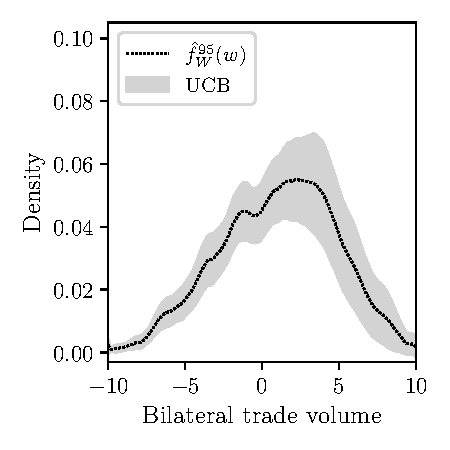
\includegraphics[scale=0.48]{graphics/trade_plot_1995.pdf}
    \caption{Year 1995, $\hat h_{\ROT} = 1.27$}
  \end{subfigure}
  %
  \begin{subfigure}{0.32\textwidth}
    \centering
    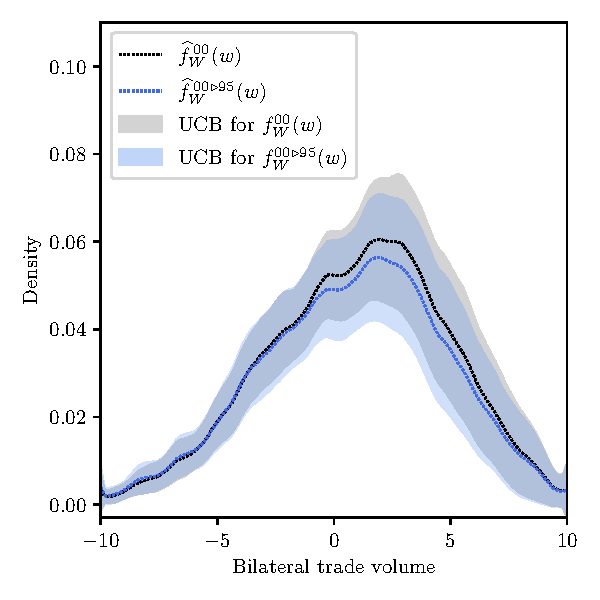
\includegraphics[scale=0.48]{graphics/trade_plot_1995_2000.pdf}
    \caption{Year 2000, $\hat h_{\ROT} = 1.31$}
  \end{subfigure}
  %
  \begin{subfigure}{0.32\textwidth}
    \centering
    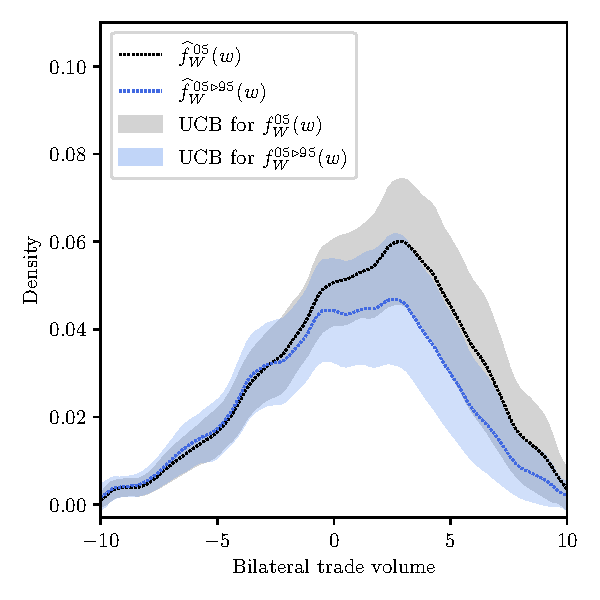
\includegraphics[scale=0.48]{graphics/trade_plot_1995_2005.pdf}
    \caption{Year 2005, $\hat h_{\ROT} = 1.37$}
  \end{subfigure}
  %
  \caption{Real and counterfactual density estimates
    and confidence bands for the DOTS data with histogram-based
  covariate estimation.}
  %
  \label{fig:app_trade}
  %
\end{figure}

\begin{figure}[ht]
  \centering
  %
  \begin{subfigure}{0.32\textwidth}
    \centering
    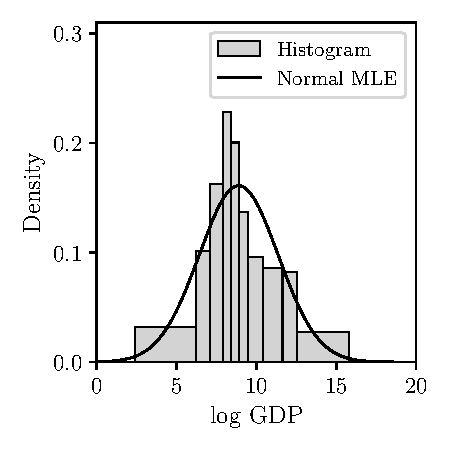
\includegraphics[scale=0.48]{graphics/trade_gdp_1995.pdf}
    \caption{Year 1995}
  \end{subfigure}
  %
  \begin{subfigure}{0.32\textwidth}
    \centering
    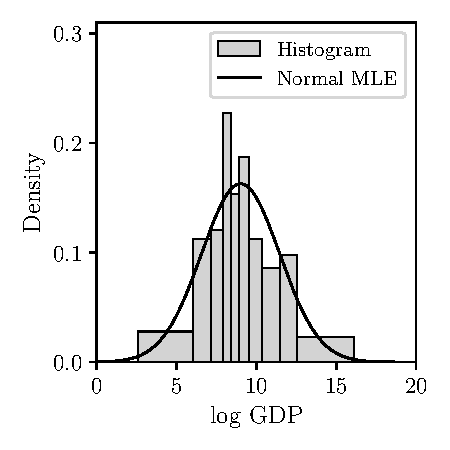
\includegraphics[scale=0.48]{graphics/trade_gdp_2000.pdf}
    \caption{Year 2000}
  \end{subfigure}
  %
  \begin{subfigure}{0.32\textwidth}
    \centering
    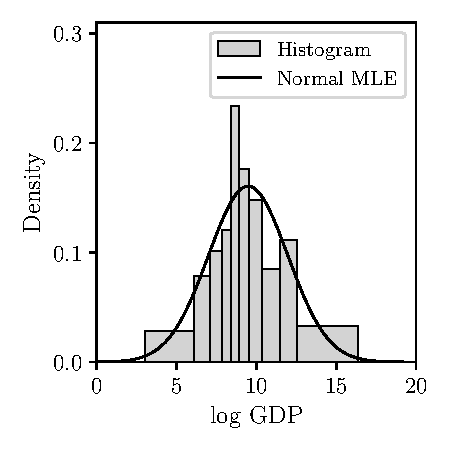
\includegraphics[scale=0.48]{graphics/trade_gdp_2005.pdf}
    \caption{Year 2005}
  \end{subfigure}
  %
  \caption{Estimated GDP distributions for the DOTS data.}
  %
  \label{fig:gdp}
  %
\end{figure}

\begin{figure}[ht]
  \centering
  %
  \begin{subfigure}{0.32\textwidth}
    \centering
    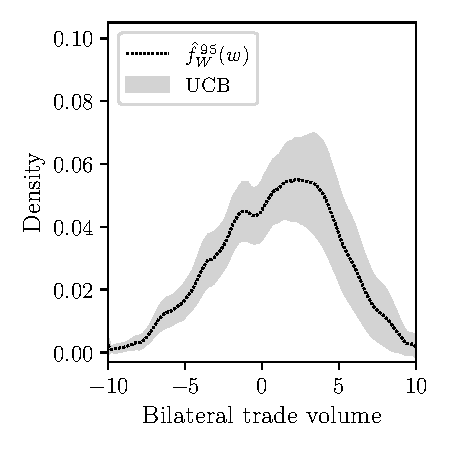
\includegraphics[scale=0.48]{graphics/trade_plot_parametric_1995.pdf}
    \caption{Year 1995, $\hat h_{\ROT} = 1.27$}
  \end{subfigure}
  %
  \begin{subfigure}{0.32\textwidth}
    \centering
    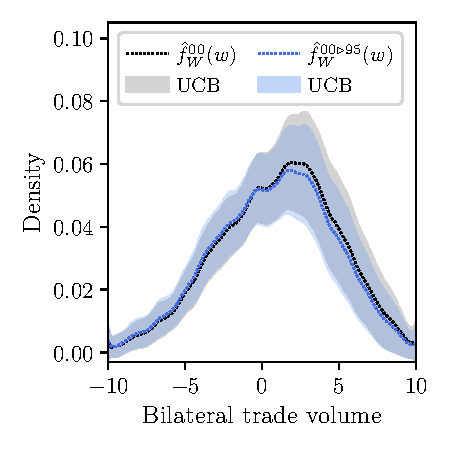
\includegraphics[scale=0.48]{graphics/trade_plot_parametric_1995_2000.pdf}
    \caption{Year 2000, $\hat h_{\ROT} = 1.31$}
  \end{subfigure}
  %
  \begin{subfigure}{0.32\textwidth}
    \centering
    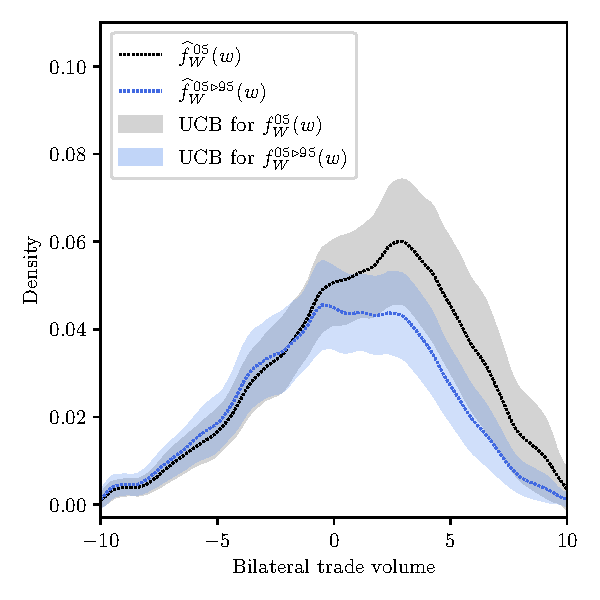
\includegraphics[scale=0.48]{graphics/trade_plot_parametric_1995_2005.pdf}
    \caption{Year 2005, $\hat h_{\ROT} = 1.37$}
  \end{subfigure}
  %
  \caption{Real and counterfactual density estimates
    and confidence bands for the DOTS data
  with parametric covariate estimation.}
  %
  \label{fig:trade_para}
  %
\end{figure}

\section{Proofs}

\subsection{Preliminary lemmas}

In this section we list some results
in probability and U-statistic theory
which are used in proofs of this paper's main results.
Other auxiliary lemmas will be introduced when
they are needed.

\subsubsection{Standard probabilistic results}

\begin{lemma}[Bernstein's inequality for independent random variables]
  \label{lem:bernstein}

  Let $X_1, \ldots, X_n$ be independent real-valued
  random variables with
  $\E[X_i] = 0$ and $|X_i| \leq M$ and
  $\E[X_i^2] \leq \sigma^2$,
  where $M$ and $\sigma$ are non-random.
  Then for all $t>0$,
  \begin{align*}
    \P \left(
      \left| \frac{1}{n} \sum_{i=1}^n X_i \right| \geq t
    \right)
    \leq 2 \exp \left( -
      \frac{t^2 n}
      {2 \sigma^2 + \frac{2}{3} M t}
    \right).
  \end{align*}

\end{lemma}

\begin{proof}[Lemma~\ref{lem:bernstein}]

  See for example
  Lemma~2.2.9 in~\citet{van1996weak}.
\end{proof}

\begin{lemma}[The matrix Bernstein inequality]
  \label{lem:matrix_bernstein}

  For $1 \leq i \leq n$
  let $X_i$ be independent symmetric $d \times d$
  real random matrices
  with expected values $\mu_i = \E[X_i]$.
  Suppose that
  $\|X_i - \mu_i\|_2 \leq M$
  almost surely for all $1 \leq i \leq n$
  where $M$ is non-random, and define
  $\sigma^2 = \big\| \sum_i \E[(X_i - \mu_i)^2] \big\|_2$.
  Then there exists a universal constant $C > 0$
  such that
  for any $t > 0$ and $q \geq 1$,
  \begin{align*}
    \P\left(
      \left\|
      \sum_{i=1}^n
      \left(
        X_i - \mu_i
      \right)
      \right\|_2
      \geq
      2 \sigma \sqrt{t}
      + \frac{4}{3} M t
    \right)
    &\leq
    2 d e^{-t}, \\
    \E\left[
      \left\|
      \sum_{i=1}^n
      \left(
        X_i - \mu_i
      \right)
      \right\|_2^q
    \right]^{1/q}
    &\leq
    C \sigma \sqrt{q + \log 2d}
    + C M (q + \log 2d).
  \end{align*}
  Another simplified version of this is as follows:
  suppose that
  $\|X_i\|_2 \leq M$ almost surely,
  so that
  $\|X_i - \mu_i\|_2 \leq 2M$.
  Then since
  $\sigma^2 \leq n M^2$,
  we have
  \begin{align*}
    \P\left(
      \left\|
      \sum_{i=1}^n
      \left(
        X_i - \mu_i
      \right)
      \right\|_2
      \geq
      4M \big(t + \sqrt{n t}\big)
    \right)
    &\leq
    2 d e^{-t}, \\
    \E\left[
      \left\|
      \sum_{i=1}^n
      \left(
        X_i - \mu_i
      \right)
      \right\|_2^q
    \right]^{1/q}
    &\leq
    C M
    \big(q + \log 2d + \sqrt{n(q + \log 2d)}\big).
  \end{align*}

\end{lemma}

\begin{proof}[Lemma~\ref{lem:matrix_bernstein}]

  See Lemma~3.2 in \citet{minsker2019moment}.
\end{proof}

\begin{lemma}[A maximal inequality for Gaussian vectors]
  \label{lem:gaussian_vector_maximal}

  Take $n \geq 2$.
  Let $X_i \sim \cN(0, \sigma_i^2)$
  for $1 \leq i \leq n$
  (not necessarily independent),
  with $\sigma_i^2 \leq \sigma^2$.
  Then
  %
  \begin{align}
    \label{eq:gaussian_vector_maximal}
    \E\left[
      \max_{1 \leq i \leq n}
      X_i
    \right]
    &\leq
    \sigma \sqrt{2 \log n}, \\
    \label{eq:gaussian_vector_maximal_abs}
    \E\left[
      \max_{1 \leq i \leq n}
      |X_i|
    \right]
    &\leq
    2 \sigma \sqrt{\log n}.
  \end{align}
  If $\Sigma_1$ and $\Sigma_2$ are constant
  positive semi-definite $n \times n$ matrices
  and $N \sim \cN(0,I_n)$,
  then
  \begin{align}
    \label{eq:gaussian_difference_psd}
    \E\Big[
      \big\|
      \Sigma_1^{1/2} N
      - \Sigma_2^{1/2} N
      \big\|_\infty
    \Big]
    &\leq
    2 \sqrt{\log n} \,
    \big\|
    \Sigma_1 - \Sigma_2
    \big\|_2^{1/2}.
  \end{align}
  %
  If further $\Sigma_1$ is
  positive definite,
  then
  %
  \begin{align}
    \label{eq:gaussian_difference_pd}
    \E\Big[
      \big\|
      \Sigma_1^{1/2} N
      - \Sigma_2^{1/2} N
      \big\|_\infty
    \Big]
    &\leq
    \sqrt{\log n} \,
    \lambda_{\min}(\Sigma_1)^{-1/2} \,
    \big\|
    \Sigma_1 - \Sigma_2
    \big\|_2.
  \end{align}

\end{lemma}

\begin{proof}[Lemma~\ref{lem:gaussian_vector_maximal}]

  For $t > 0$,
  Jensen's inequality on the concave logarithm function
  gives
  \begin{align*}
    \E\left[
      \max_{1 \leq i \leq n}
      X_i
    \right]
    &=
    \frac{1}{t}
    \E\left[
      \log
      \exp
      \max_{1 \leq i \leq n}
      t X_i
    \right]
    \leq
    \frac{1}{t}
    \log
    \E\left[
      \exp
      \max_{1 \leq i \leq n}
      t X_i
    \right]
    \leq
    \frac{1}{t}
    \log
    \sum_{i=1}^n
    \E\left[
      \exp
      t X_i
    \right] \\
    &=
    \frac{1}{t}
    \log
    \sum_{i=1}^n
    \exp
    \left(
      \frac{t^2 \sigma_i^2}{2}
    \right)
    \leq
    \frac{1}{t}
    \log n
    + \frac{t \sigma^2}{2},
  \end{align*}
  where we use the Gaussian moment generating function.
  Minimizing this upper bound over $t$
  by setting $t = \sqrt{2 \log n} / \sigma$
  yields Equation~\ref{eq:gaussian_vector_maximal}:
  \begin{align*}
    \E\left[
      \max_{1 \leq i \leq n}
      X_i
    \right]
    &\leq
    \sigma \sqrt{2 \log n}.
  \end{align*}
  For Equation~\ref{eq:gaussian_vector_maximal_abs},
  we use the symmetry of the Gaussian distribution:
  \begin{align*}
    \E\left[
      \max_{1 \leq i \leq n}
      |X_i|
    \right]
    &=
    \E\left[
      \max_{1 \leq i \leq n}
      \{X_i, -X_i\}
    \right]
    \leq
    \sigma \sqrt{2 \log 2n}
    \leq
    2 \sigma \sqrt{\log n}.
  \end{align*}
  For
  Equations~\ref{eq:gaussian_difference_psd}
  and~\ref{eq:gaussian_difference_pd},
  note that
  $\Sigma_1^{1/2} N - \Sigma_2^{1/2} N$
  is a Gaussian vector with covariance matrix
  $\big(\Sigma_1^{1/2} - \Sigma_2^{1/2}\big)^2$.
  The variances of of its components are the diagonal
  elements of this matrix, namely
  \begin{align*}
    \sigma_i^2
    &=
    \Var\big[
      \big(\Sigma_1^{1/2} N - \Sigma_2^{1/2} N\big)_i
    \big]
    =
    \Big(\big(
        \Sigma_1^{1/2} - \Sigma_2^{1/2}
    \big)^2\Big)_{ii}.
  \end{align*}
  Note that if $e_i$ is the
  $i$th standard unit basis vector,
  then for any real symmetric matrix $A$,
  we have
  $e_i^\T A^2 e_i = (A^2)_{ii}$,
  so in particular
  $(A^2)_{ii} \leq \|A\|_2^2$.
  Therefore
  \begin{align*}
    \sigma_i^2
    &\leq
    \big\|
    \Sigma_1^{1/2} - \Sigma_2^{1/2}
    \big\|_2^2
    =\vcentcolon
    \sigma^2.
  \end{align*}
  Applying
  Equation~\ref{eq:gaussian_vector_maximal_abs}
  then gives
  \begin{align*}
    \E\Big[
      \big\|
      \Sigma_1^{1/2} N
      - \Sigma_2^{1/2} N
      \big\|_\infty
    \Big]
    &\leq
    2 \sqrt{\log n} \,
    \big\|
    \Sigma_1^{1/2} - \Sigma_2^{1/2}
    \big\|_2.
  \end{align*}
  By Theorem~X.1.1
  in \citet{bhatia1997matrix},
  we can deduce
  \begin{align*}
    \big\|
    \Sigma_1^{1/2} - \Sigma_2^{1/2}
    \big\|_2
    &\leq
    \big\|
    \Sigma_1 - \Sigma_2
    \big\|_2^{1/2},
  \end{align*}
  giving
  Equation~\ref{eq:gaussian_difference_psd}.
  If further $\Sigma_1$
  is positive definite,
  then by
  Theorem~X.3.8 in
  \citet{bhatia1997matrix},
  \begin{align*}
    \big\|
    \Sigma_1^{1/2} - \Sigma_2^{1/2}
    \big\|_2
    &\leq
    \frac{1}{2}
    \lambda_{\min}(\Sigma_1)^{-1/2} \,
    \big\|
    \Sigma_1 - \Sigma_2
    \big\|_2,
  \end{align*}
  giving
  Equation~\ref{eq:gaussian_difference_pd}.
\end{proof}

\begin{lemma}[Maximal inequalities for Gaussian processes]
  \label{lem:gaussian_process_maximal}

  Let $Z$ be a separable
  mean-zero Gaussian process indexed
  by $x \in \cX$.
  Recall that $Z$ is separable for example if
  $\cX$ is Polish
  and $Z$ has
  continuous trajectories.
  Define its covariance structure on $\cX \times \cX$
  by $\Sigma(x, x') = \E[Z(x) Z(x')]$,
  and the corresponding semimetric on $\cX$
  by
  \begin{align*}
    \rho(x,x')
    &=
    \E\big[\big(Z(x) - Z(x')\big)^2\big]^{1/2}
    = \big(\Sigma(x,x)
      - 2 \Sigma(x,x')
    + \Sigma(x',x')\big)^{1/2}.
  \end{align*}
  Let $N(\varepsilon, \cX, \rho)$
  denote the $\varepsilon$-covering number of $\cX$
  with respect to the semimetric $\rho$.
  Define $\sigma = \sup_x \Sigma(x,x)^{1/2}$.
  Then there exists a universal constant $C > 0$
  such that for any $\delta > 0$,
  \begin{align*}
    \E\left[
      \sup_{x \in \cX}
      |Z(x)|
    \right]
    &\leq
    C \sigma
    + C \int_0^{2\sigma}
    \sqrt{\log N(\varepsilon, \cX, \rho)}
    \diff{\varepsilon}, \\
    \E\left[
      \sup_{\rho(x,x') \leq \delta}
      |Z(x) - Z(x')|
    \right]
    &\leq
    C \int_0^{\delta}
    \sqrt{\log N(\varepsilon, \cX, \rho)}
    \diff{\varepsilon}.
  \end{align*}

\end{lemma}

\begin{proof}[Lemma~\ref{lem:gaussian_process_maximal}]

  See Corollary~2.2.8 in \citet{van1996weak},
  noting that for any $x,x' \in \cX$, we have
  $\E[|Z(x)|] \lesssim \sigma$ and
  $\rho(x,x') \leq 2\sigma$,
  implying that
  $\log N(\varepsilon, \cX, \rho) = 0$
  for all
  $\varepsilon > 2 \sigma$.
\end{proof}

\begin{lemma}[Anti-concentration for Gaussian process absolute suprema]
  \label{lem:anti-concentration}

  Let $Z$ be a separable mean-zero Gaussian process
  indexed by a semimetric space $\cX$ with
  $\E[Z(x)^2] = 1$
  for all $x \in \cX$.
  Then for any $\varepsilon > 0$,
  \begin{align*}
    \sup_{t \in \R}
    \P\left(
      \left|
      \sup_{x \in \cX}
      \big| Z(x) \big|
      - t
      \right|
      \leq \varepsilon
    \right)
    &\leq
    4 \varepsilon
    \left(
      1 + \E\left[
        \sup_{x \in \cX}
        \big| Z(x) \big|
      \right]
    \right).
  \end{align*}

\end{lemma}

\begin{proof}[Lemma~\ref{lem:anti-concentration}]

  See Corollary~2.1
  in \citet{chernozhukov2014anti}.
\end{proof}

\begin{lemma}[No slowest rate of convergence in probability]
  \label{lem:slow_convergence}

  Let $X_n$ be a sequence of real-valued random
  variables with
  $X_n = o_\P(1)$.
  Then there exists a deterministic sequence
  $\varepsilon_n \to 0$
  such that
  $\P\big(|X_n| > \varepsilon_n\big) \leq \varepsilon_n$
  for all $n \geq 1$.

\end{lemma}

\begin{proof}[Lemma~\ref{lem:slow_convergence}]

  Define the following deterministic sequence
  for $k \geq 1$.
  \begin{align*}
    \tau_k
    &=
    \sup
    \big\{
      n \geq 1:
      \P\big(|X_n| > 1/k\big)
      > 1/k
    \big\}
    \vee
    (\tau_{k-1} +1)
  \end{align*}
  with $\tau_0 = 0$.
  Since $X_n = o_\P(1)$,
  each $\tau_k$ is finite
  and so we can define
  $\varepsilon_n = \frac{1}{k}$
  where $\tau_k < n \leq \tau_{k+1}$.
  Then, noting that $\varepsilon_n \to 0$,
  we have
  $\P\big(|X_n| > \varepsilon_n\big)
  = \P\big(|X_n| > 1/k\big) \leq 1/k = \varepsilon_n$.
\end{proof}

\subsubsection{U-statistics}

\begin{lemma}[General Hoeffding-type decomposition]
  \label{lem:general_hoeffding}

  Let $\cU$ be a vector space.
  Let $u_{i j} \in \cU$ be defined for
  $1 \leq i, j \leq n$
  and
  $i \neq j$.
  Suppose that $u_{i j} = u_{j i}$
  for all $i,j$.
  Then for any $u_i \in \cU$
  (for $1 \leq i \leq n$)
  and any $u \in \cU$,
  the following decomposition holds:
  \begin{align*}
    \sum_{i=1}^n
    \sum_{\substack{j=1 \\ j \neq i}}^n
    \big(u_{i j} - u\big)
    &=
    2(n-1)
    \sum_{i=1}^n
    \big(u_i - u\big)
    +
    \sum_{i=1}^n
    \sum_{\substack{j=1 \\ j \neq i}}^n
    \big(u_{i j} - u_i - u_j + u\big).
  \end{align*}

\end{lemma}

\begin{proof}[Lemma~\ref{lem:general_hoeffding}]

  We compute the left hand side minus the right hand side,
  beginning by observing that all of the
  $u_{i j}$ and $u$ terms clearly cancel.
  \begin{align*}
    &\sum_{i=1}^n
    \sum_{\substack{j=1 \\ j \neq i}}^n
    \big(u_{i j} - u\big)
    - 2(n-1)
    \sum_{i=1}^n
    \big(u_i - u\big)
    -
    \sum_{i=1}^n
    \sum_{j \neq i}
    \big(u_{i j} - u_i - u_j + u\big) \\
    &\qquad=
    - 2(n-1)
    \sum_{i=1}^n
    u_i
    -
    \sum_{i=1}^n
    \sum_{\substack{j=1 \\ j \neq i}}^n
    \big(- u_i - u_j\big)
    =
    - 2(n-1)
    \sum_{i=1}^n
    u_i
    +
    \sum_{i=1}^n
    \sum_{\substack{j=1 \\ j \neq i}}^n
    u_i
    +
    \sum_{j=1}^n
    \sum_{\substack{i=1 \\ i \neq j}}^n
    u_j \\
    &\qquad=
    - 2(n-1)
    \sum_{i=1}^n
    u_i
    +
    (n-1)
    \sum_{i=1}^n
    u_i
    +
    (n-1)
    \sum_{j=1}^n
    u_j
    = 0.
  \end{align*}
\end{proof}

\begin{lemma}[A U-statistic concentration inequality]
  \label{lem:ustat_concentration}

  Let $(S,\cS)$ be a measurable space and
  $X_1, \ldots, X_n$ be i.i.d.\ $S$-valued random variables.
  Let $H: S^m \to \R$ be a function of $m$ variables
  satisfying the symmetry property
  $H(x_1, \ldots, x_m) = H(x_{\tau (1)}, \ldots, x_{\tau (m)})$
  for any $m$-permutation $\tau$.
  Suppose also that
  $\E[H(X_1, \ldots, X_m)] = 0$.
  Let
  $M = \|H\|_\infty$
  and
  $\sigma^2 = \E\big[\E[H(X_1, \ldots, X_m) \mid X_1]^2\big]$.
  Define the (not necessarily degenerate)
  U-statistic
  \begin{align*}
    U_n
    &=
    \frac{m!(n-m)!}{n!}
    \sum_{1 \leq i_1 < \cdots < i_m \leq n}
    H(X_1, \ldots, X_n).
  \end{align*}
  Then for any $t > 0$,
  \begin{align*}
    \P\left(
      |U_n| > t
    \right)
    &\leq
    4 \exp \left(
      - \frac{n t^2}{C_1(m) \sigma^2 + C_2(m) M t}
    \right),
  \end{align*}
  where $C_1(m)$, $C_2(m)$
  are positive constants depending only on $m$.

\end{lemma}

\begin{proof}[Lemma~\ref{lem:ustat_concentration}]

  See Theorem~2 in \citet{arcones1995bernstein}.
\end{proof}

\begin{lemma}[A second-order U-process maximal inequality]
  \label{lem:uprocess_maximal}

  Let $X_1 \ldots, X_n$
  be i.i.d.\ random variables taking values
  in a measurable space $(S, \cS)$
  with distribution $\P$.
  Let $\cF$ be a class of measurable functions from
  $S \times S$ to $\R$ which is also pointwise measurable.
  Define the degenerate second-order U-process
  \begin{align*}
    U_n(f)
    &=
    \frac{2}{n(n-1)}
    \sum_{i<j}
    \Big(
      f(X_i, X_j)
      - \E\big[f(X_i,X_j) \mid X_i\big]
      - \E\big[f(X_i,X_j) \mid X_j\big]
      + \E\big[f(X_i,X_j)\big]
    \Big)
  \end{align*}
  for $f \in \cF$.
  Suppose that each $f \in \cF$ is symmetric in the sense that
  $f(s_1,s_2) = f(s_2,s_1)$
  for all $s_1, s_2 \in S$.
  Let $F$ be a measurable envelope function for $\cF$
  satisfying $|f(s_1,s_2)| \leq F(s_1,s_2)$
  for all $s_1,s_2 \in S$.
  For a law $\Q$ on
  $(S \times S, \, \cS \otimes \cS)$,
  define the $(\Q,q)$-norm of $f \in \cF$ by
  $\|f\|_{\Q,q}^q = \E_\Q[|f|^q]$.
  Assume that $\cF$ is VC-type in the following manner.
  \begin{align*}
    \sup_\Q
    N\big(
      \cF, \|\cdot\|_{\Q,2}, \varepsilon \|F\|_{\Q,2}
    \big)
    &\leq
    (C_1/\varepsilon)^{C_2}
  \end{align*}
  for some constants
  $C_1 \geq e$
  and
  $C_2 \geq 1$,
  and for all $\varepsilon \in (0,1]$,
  where $\Q$ ranges over all finite discrete laws
  on
  $S \times S$.
  Let $\sigma > 0$ be any deterministic value satisfying
  $\sup_{f \in \cF} \|f\|_{\P,2} \leq \sigma \leq \|F\|_{\P,2}$,
  and define the random variable $M = \max_{i,j} |F(X_i, X_j)|$.
  Then there exists a universal constant $C_3 > 0$
  satisfying
  \begin{align*}
    n
    \E\left[
      \sup_{f \in \cF}
      \big| U_n(f) \big|
    \right]
    &\leq
    C_3 \sigma
    \Big(
      C_2 \log\big(C_1 \|F\|_{\P,2} / \sigma \big)
    \Big)
    + \frac{C_3 \|M\|_{\P,2}}{\sqrt{n}}
    \Big(
      C_2 \log\big(C_1 \|F\|_{\P,2} / \sigma \big)
    \Big)^2.
  \end{align*}

\end{lemma}

\begin{proof}[Lemma~\ref{lem:uprocess_maximal}]

  Apply Corollary~5.3
  from \citet{chen2020jackknife}
  with the order of the U-statistic fixed at
  $r=2$,
  and with $k=2$.
\end{proof}

\begin{lemma}[A U-statistic matrix concentration inequality]
  \label{lem:ustat_matrix_concentration}

  Let $X_1, \ldots, X_n$ be i.i.d.\ random variables
  taking values in a measurable space $(S, \cS)$.
  Suppose
  $H: S^2 \to \R^{d \times d}$
  is a measurable matrix-valued function
  of two variables
  satisfying the following assumptions:
  \begin{enumerate}[label=(\roman*)]

    \item
      $H(X_1, X_2)$ is an almost surely symmetric matrix.

    \item
      $\|H(X_1, X_2)\|_2 \leq M$ almost surely.

    \item
      $H$ is a symmetric function in its arguments in that
      $H(X_1, X_2) = H(X_2, X_1)$ almost surely.

    \item
      $H$ is degenerate in the sense that
      $\E[H(X_1, x_2)] = 0$ for all $x_2 \in S$.

  \end{enumerate}
  Let $U_n = \sum_i \sum_{j \neq i} H(X_i, X_j)$
  be a U-statistic,
  and define the variance-type constant
  \begin{align*}
    \sigma^2
    &=
    \E\left[
      \left\|
      \E\left[
        H(X_i, X_j)^2
        \mid X_j
      \right]
      \right\|_2
    \right].
  \end{align*}
  Then for a universal constant $C > 0$
  and for all $t > 0$,
  \begin{align*}
    \P\left(
      \|U_n\|_2
      \geq
      C \sigma n (t + \log d)
      + C M \sqrt{n} (t + \log d)^{3/2}
    \right)
    &\leq
    C e^{-t}.
  \end{align*}
  We remark here that clearly
  by Jensen's inequality,
  $\sigma^2 \leq \E[ \| H(X_i, X_j)^2 \|_2 ]
  = \E[ \| H(X_i, X_j) \|_2^2 ]
  \leq M^2$,
  giving the weaker but simpler concentration inequality
  \begin{align*}
    \P\left(
      \|U_n\|_2
      \geq
      2 C M n
      (t + \log d)^{3/2}
    \right)
    &\leq
    C e^{-t}.
  \end{align*}
  From this last inequality we can deduce the following moment bound
  by integration of tail probabilities.
  \begin{align*}
    \E\left[
      \|U_n\|_2
    \right]
    &\lesssim
    M n (\log d)^{3/2}.
  \end{align*}

\end{lemma}

\begin{proof}[Lemma~\ref{lem:ustat_matrix_concentration}]

  We apply results from \citet{minsker2019moment}.

  \proofparagraph{decoupling}

  Let $\bar U_n = \sum_{i=1}^n \sum_{j=1}^n H(X_i^{(1)}, X_j^{(2)})$
  be a decoupled matrix U-statistic,
  where $X^{(1)}$ and $X^{(2)}$
  are i.i.d.\ copies of the sequence $X_1, \ldots, X_n$.
  By Lemma~5.2 in \citet{minsker2019moment},
  since we are only stating this result for
  degenerate U-statistics of order 2,
  there exists a universal constant $D_2$
  such that for any $t > 0$,
  we have
  \begin{align*}
    \P\left(
      \|U_n\|_2 \geq t
    \right)
    &\leq
    D_2
    \P\left(
      \|\bar U_n\|_2 \geq t / D_2
    \right).
  \end{align*}

  \proofparagraph{concentration of the decoupled U-statistic}

  By Equation~11 in \citet{minsker2019moment},
  we have the following concentration inequality
  for decoupled degenerate U-statistics.
  For some universal constant $C_1$
  and for any $t > 0$,
  \begin{align*}
    \P\left(
      \|\bar U_n\|_2
      \geq
      C_1 \sigma n (t + \log d)
      + C_1 M \sqrt{n} (t + \log d)^{3/2}
    \right)
    &\leq
    e^{-t}.
  \end{align*}

  \proofparagraph{concentration of the original U-statistic}

  Hence we have
  \begin{align*}
    &\P\left(
      \|U_n\|_2
      \geq
      C_1 D_2 \sigma n (t + \log d)
      + C_1 D_2 M \sqrt{n} (t + \log d)^{3/2}
    \right) \\
    &\quad\leq
    D_2 \P\left(
      \|\bar U_n\|_2
      \geq
      C_1 \sigma n (t + \log d)
      + C_1 M \sqrt{n} (t + \log d)^{3/2}
    \right) \\
    &\quad\leq
    D_2 e^{-t}.
  \end{align*}
  The main result follows by setting
  $C = C_1 + C_1 D_2$.

  \proofparagraph{moment bound}

  The final equation,
  giving a moment bound for the simplified version,
  can be deduced as follows.
  We already have that
  \begin{align*}
    \P\left(
      \|U_n\|_2
      \geq
      2 C M n
      (t + \log d)^{3/2}
    \right)
    &\leq
    C e^{-t}.
  \end{align*}
  This implies that for any $t \geq \log d$,
  we have
  \begin{align*}
    \P\left(
      \|U_n\|_2
      \geq
      8 C M n
      t^{3/2}
    \right)
    &\leq
    C e^{-t}.
  \end{align*}
  Defining
  $s = 8 C M n t^{3/2}$,
  or equivalently
  $t = \left( \frac{s}{8C M n} \right)^{2/3}$,
  shows that
  for any $s \geq 8C M n(\log d)^{3/2}$,
  \begin{align*}
    \P\left(
      \|U_n\|_2
      \geq
      s
    \right)
    &\leq
    C e^{-\left( \frac{s}{8C M n} \right)^{2/3}}.
  \end{align*}
  %
  Hence the moment bound is obtained:
  %
  \begin{align*}
    \E\left[
      \|U_n\|_2
    \right]
    &=
    \int_0^\infty
    \P\left(
      \|U_n\|_2
      \geq
      s
    \right)
    \diff{s} \\
    &=
    \int_0^{8C M n(\log d)^{3/2}}
    \P\left(
      \|U_n\|_2
      \geq
      s
    \right)
    \diff{s}
    +
    \int_{8C M n(\log d)^{3/2}}^\infty
    \P\left(
      \|U_n\|_2
      \geq
      s
    \right)
    \diff{s} \\
    &\leq
    8C M n(\log d)^{3/2}
    +
    \int_0^\infty
    C e^{-\left( \frac{s}{8C M n} \right)^{2/3}}
    \diff{s}
    =
    8C M n(\log d)^{3/2}
    +
    8C M n
    \int_0^\infty
    e^{s^{-2/3}}
    \diff{s} \\
    &\lesssim
    Mn(\log d)^{3/2}.
  \end{align*}
\end{proof}

\subsection{Technical results}

\subsubsection{Maximal inequalities for i.n.i.d.\ empirical processes}

Before presenting the proof of
Lemma~\ref{lem:maximal_entropy},
we give some auxiliary lemmas;
namely a symmetrization inequality
(Lemma~\ref{lem:symmetrization}),
a Rademacher contraction principle
(Lemma~\ref{lem:contraction})
and a Hoffman--J{\o}rgensen inequality
(Lemma~\ref{lem:hoffmann}).
Recall that the Rademacher distribution
places probability mass of $1/2$
on each of the points $-1$ and $1$.

\begin{lemma}[A symmetrization inequality for i.n.i.d.\ variables]
  \label{lem:symmetrization}

  Let $(S, \cS)$ be a measurable space and
  $\cF$ a class of Borel-measurable functions
  from $S$ to $\R$ which is pointwise measurable
  (i.e.\ it contains a countable dense subset
  under pointwise convergence).
  Let $X_1, \ldots, X_n$
  be independent
  but not necessarily identically distributed
  $S$-valued random variables.
  Let $a_1, \ldots, a_n$ be arbitrary points in $S$
  and $\phi$ a non-negative non-decreasing convex function
  from $\R$ to $\R$.
  Define $\varepsilon_1, \ldots, \varepsilon_n$
  as independent Rademacher
  random variables,
  independent of $X_1, \ldots, X_n$.
  Then
  \begin{align*}
    \E \left[
      \phi \left(
        \sup_{f \in \cF}
        \left|
        \sum_{i=1}^n
        \Big(
          f(X_i)
          - \E[f(X_i)]
        \Big)
        \right|
      \right)
    \right]
    &\leq
    \E \left[
      \phi \left(
        2
        \sup_{f \in \cF}
        \left|
        \sum_{i=1}^n
        \varepsilon_i
        \Big(
          f(X_i)
          - a_i
        \Big)
        \right|
      \right)
    \right].
  \end{align*}
  Note that in particular this holds with $a_i = 0$
  and also holds with $\phi(t) = t \vee 0$.

\end{lemma}

\begin{proof}[Lemma~\ref{lem:symmetrization}]

  See Lemma~2.3.6 in
  \citet{van1996weak}.
  %
\end{proof}

\begin{lemma}[A Rademacher contraction principle]
  \label{lem:contraction}

  Let $\varepsilon_1, \ldots, \varepsilon_n$
  be independent Rademacher random variables
  and $\cT$ be a bounded subset of $\R^n$.
  Define
  $M = \sup_{t \in \cT} \max_{1 \leq i \leq n} |t_i|$.
  Then, noting that the supremum is measurable
  because $\cT$ is a subset of a separable metric space
  and is therefore itself separable,
  \begin{align*}
    \E
    \left[
      \sup_{t \in \cT}
      \left|
      \sum_{i=1}^n
      \varepsilon_i
      t_i^2
      \right|
    \right]
    &\leq
    4M \,
    \E
    \left[
      \sup_{t \in \cT}
      \left|
      \sum_{i=1}^n
      \varepsilon_i
      t_i
      \right|
    \right].
  \end{align*}
  This gives the following corollary.
  Let $X_1, \ldots, X_n$ be mutually independent
  and also independent of $\varepsilon_1, \ldots, \varepsilon_n$.
  Let $\cF$ be a pointwise measurable class of functions
  from a measurable space $(S, \cS)$ to $\R$,
  with measurable envelope $F$.
  Define $M = \max_i F(X_i)$.
  Then we obtain that
  \begin{align*}
    \E
    \left[
      \sup_{f \in \cF}
      \left|
      \sum_{i=1}^n
      \varepsilon_i
      f(X_i)^2
      \right|
    \right]
    &\leq
    4
    \E
    \left[
      M
      \sup_{f \in \cF}
      \left|
      \sum_{i=1}^n
      \varepsilon_i
      f(X_i)
      \right|
    \right].
  \end{align*}

\end{lemma}

\begin{proof}[Lemma~\ref{lem:contraction}]

  We apply Theorem~4.12
  from \citet{ledoux1991probability}
  with $F$ as the identity function
  and
  \begin{align*}
    \psi_i(s)
    = \psi(s)
    &=
    \min
    \left(
      \frac{s^2}{2M},
      \frac{M}{2}
    \right).
  \end{align*}
  This is a weak contraction
  (i.e.\ 1-Lipschitz)
  because it is continuous,
  differentiable on $(-M,M)$
  with derivative bounded by
  $|\psi'(s)| \leq |s|/M \leq 1$,
  and constant outside $(-M,M)$.
  Note that since $|t_i| \leq M$
  by definition,
  we have $\psi_i(t_i) = t_i^2 / (2M)$.
  Hence
  by Theorem~4.12
  from \citet{ledoux1991probability},
  \begin{align*}
    \E
    \left[
      F
      \left(
        \frac{1}{2}
        \sup_{t \in \cT}
        \left|
        \sum_{i=1}^n
        \varepsilon_i
        \psi_i(t_i)
        \right|
      \right)
    \right]
    &\leq
    \E
    \left[
      F
      \left(
        \sup_{t \in \cT}
        \left|
        \sum_{i=1}^n
        \varepsilon_i
        t_i
        \right|
      \right)
    \right], \\
    \E
    \left[
      \frac{1}{2}
      \sup_{t \in \cT}
      \left|
      \sum_{i=1}^n
      \varepsilon_i
      \frac{t_i^2}{2M}
      \right|
    \right]
    &\leq
    \E
    \left[
      \sup_{t \in \cT}
      \left|
      \sum_{i=1}^n
      \varepsilon_i
      t_i
      \right|
    \right], \\
    \E
    \left[
      \sup_{t \in \cT}
      \left|
      \sum_{i=1}^n
      \varepsilon_i
      t_i^2
      \right|
    \right]
    &\leq
    4M \,
    \E
    \left[
      \sup_{t \in \cT}
      \left|
      \sum_{i=1}^n
      \varepsilon_i
      t_i
      \right|
    \right].
  \end{align*}
  %
  To see the corollary,
  set
  $\cT = \left\{\big(f(X_1), \ldots, f(X_n)\big) : f \in \cF\right\}$
  and note that for fixed realization
  $X_1, \ldots, X_n$,
  \begin{align*}
    \E_\varepsilon
    \left[
      \sup_{f \in \cF}
      \left|
      \sum_{i=1}^n
      \varepsilon_i
      f(X_i)^2
      \right|
    \right]
    &=
    \E_\varepsilon
    \left[
      \sup_{t \in \cT}
      \left|
      \sum_{i=1}^n
      \varepsilon_i
      t_i^2
      \right|
    \right] \\
    &\leq 4
    \E_\varepsilon
    \left[
      M
      \sup_{t \in \cT}
      \left|
      \sum_{i=1}^n
      \varepsilon_i
      t_i
      \right|
    \right]
    = 4 \E_\varepsilon
    \left[
      M
      \sup_{f \in \cF}
      \left|
      \sum_{i=1}^n
      \varepsilon_i
      f(X_i)
      \right|
    \right].
  \end{align*}
  %
  Taking an expectation over $X_1, \ldots, X_n$
  and applying Fubini's theorem yields the result.
\end{proof}

\begin{lemma}[A Hoffmann--J{\o}rgensen inequality]
  \label{lem:hoffmann}

  Let $(S, \cS)$ be a measurable space
  and $X_1, \ldots, X_n$
  be $S$-valued random variables.
  Suppose that
  $\cF$ is a pointwise measurable class of functions from $S$ to $\R$
  with finite envelope $F$.
  Let $\varepsilon_1, \ldots, \varepsilon_n$
  be independent Rademacher random variables
  which are independent of $X_1, \ldots, X_n$.
  Then for any $q \in (1, \infty)$,
  \begin{align*}
    \E \left[
      \sup_{f \in \cF}
      \left|
      \sum_{i=1}^n
      \varepsilon_i
      f(X_i)
      \right|
      ^q
    \right]
    ^{1/q}
    &\leq
    C_q
    \left(
      \E \left[
        \sup_{f \in \cF}
        \left|
        \sum_{i=1}^n
        \varepsilon_i
        f(X_i)
        \right|
      \right]
      +
      \E \left[
        \max_{1 \leq i \leq n}
        \sup_{f \in \cF}
        \big| f(X_i) \big|^q
      \right]^{1/q}
    \right),
  \end{align*}
  where $C_q$ is a positive constant depending only on $q$.

\end{lemma}

\begin{proof}[Lemma~\ref{lem:hoffmann}]

  We use Talagrand's formulation of
  a Hoffmann--J{\o}rgensen inequality.
  Consider the
  independent
  $\ell^\infty(\cF)$-valued
  random functionals $u_i$ defined by
  $u_i(f) = \varepsilon_i f(X_i)$,
  where $\ell^\infty(\cF)$
  is the Banach space of bounded functions from
  $\cF$ to $\R$,
  equipped with the norm
  $\|u\|_\cF = \sup_{f \in \cF} |u(f)|$.
  Then Remark~3.4 in \citet{kwapien1991hypercontraction} gives
  \begin{align*}
    \E \left[
      \sup_{f \in \cF}
      \left|
      \sum_{i=1}^n
      u_i(f)
      \right|
      ^q
    \right]
    ^{1/q}
    &\leq
    C_q
    \left(
      \E \left[
        \sup_{f \in \cF}
        \left|
        \sum_{i=1}^n
        u_i(f)
        \right|
      \right]
      +
      \E \left[
        \max_{1 \leq i \leq n}
        \sup_{f \in \cF}
        \left|
        u_i(f)
        \right|^q
      \right]^{1/q}
    \right) \\
    \E \left[
      \sup_{f \in \cF}
      \left|
      \sum_{i=1}^n
      \varepsilon_i
      f(X_i)
      \right|
      ^q
    \right]
    ^{1/q}
    &\leq
    C_q
    \left(
      \E \left[
        \sup_{f \in \cF}
        \left|
        \sum_{i=1}^n
        \varepsilon_i
        f(X_i)
        \right|
      \right]
      +
      \E \left[
        \max_{1 \leq i \leq n}
        \sup_{f \in \cF}
        \big| f(X_i) \big|^q
      \right]^{1/q}
    \right).
  \end{align*}
\end{proof}

\begin{proof}[Lemma~\ref{lem:maximal_entropy}]

  We follow the proof of Theorem~5.2
  from \citet{chernozhukov2014gaussian},
  using our i.n.i.d.\ versions of the symmetrization inequality
  (Lemma~\ref{lem:symmetrization}),
  Rademacher contraction principle
  (Lemma~\ref{lem:contraction})
  and Hoffmann--J{\o}rgensen inequality
  (Lemma~\ref{lem:hoffmann}).

  Without loss of generality,
  we may assume that $J(1, \cF, F) < \infty$
  as otherwise there is nothing to prove,
  and that $F > 0$ everywhere on $S$.
  Let $\P_n = n^{-1} \sum_i \delta_{X_i}$
  be the empirical distribution
  of $X_i$,
  and define the empirical variance bound
  $\sigma_n^2 = \sup_\cF n^{-1} \sum_i f(X_i)^2$.
  By the i.n.i.d.\ symmetrization inequality
  (Lemma~\ref{lem:symmetrization}),
  \begin{align*}
    \E \left[
      \sup_{f \in \cF}
      \big| G_n(f) \big|
    \right]
    &=
    \frac{1}{\sqrt n}
    \E \left[
      \sup_{f \in \cF}
      \left|
      \sum_{i=1}^n
      \Big(
        f(X_i)
        - \E[f(X_i)]
      \Big)
      \right|
    \right]
    \leq
    \frac{2}{\sqrt n}
    \E \left[
      \sup_{f \in \cF}
      \left|
      \sum_{i=1}^n
      \varepsilon_i
      f(X_i)
      \right|
    \right],
  \end{align*}
  %
  where $\varepsilon_1, \ldots, \varepsilon_n$
  are independent Rademacher random variables,
  independent of $X_1, \ldots, X_n$.
  Then the standard entropy integral inequality
  from the proof of Theorem~5.2 in
  the supplemental materials for
  \citet{chernozhukov2014gaussian}
  gives for a universal constant $C_1 > 0$,
  %
  \begin{align*}
    \frac{1}{\sqrt n}
    \E \left[
      \sup_{f \in \cF}
      \left|
      \sum_{i=1}^n
      \varepsilon_i
      f(X_i)
      \right|
      \Bigm\vert
      X_1, \ldots, X_n
    \right]
    &\leq
    C_1 \|F\|_{\P_n,2}
    J(\sigma_n / \|F\|_{\P_n,2}, \cF, F).
  \end{align*}
  %
  Taking marginal expectations
  and applying Jensen's inequality along with
  a convexity result for the covering integral,
  as in Lemma~A.2 in \citet{chernozhukov2014gaussian},
  gives
  %
  \begin{align*}
    Z
    &\vcentcolon=
    \frac{1}{\sqrt n}
    \E \left[
      \sup_{f \in \cF}
      \left|
      \sum_{i=1}^n
      \varepsilon_i
      f(X_i)
      \right|
    \right]
    \leq
    C_1 \|F\|_{\bar\P,2}
    J(\E[\sigma_n^2]^{1/2} / \|F\|_{\bar\P,2}, \cF, F).
  \end{align*}
  %
  Next use the symmetrization inequality
  (Lemma~\ref{lem:symmetrization}),
  the contraction principle
  (Lemma~\ref{lem:contraction}),
  the Cauchy--Schwarz inequality
  and the Hoffmann--J{\o}rgensen inequality
  (Lemma~\ref{lem:hoffmann})
  to deduce that
  %
  \begin{align*}
    \E[\sigma_n^2]
    &=
    \E\left[
      \sup_{f \in \cF}
      \frac{1}{n}
      \sum_{i=1}^n
      f(X_i)^2
    \right]
    \leq
    \sup_{f \in \cF}
    \E_{\bar\P} \left[
      f(X_i)^2
    \right]
    + \frac{1}{n}
    \E\left[
      \sup_{f \in \cF}
      \left|
      \sum_{i=1}^n
      f(X_i)^2
      - \E \left[
        f(X_i)^2
      \right]
      \right|
    \right] \\
    &\leq
    \sigma^2
    + \frac{2}{n}
    \E\left[
      \sup_{f \in \cF}
      \left|
      \sum_{i=1}^n
      \varepsilon_i
      f(X_i)^2
      \right|
    \right]
    \leq
    \sigma^2
    + \frac{8}{n}
    \E\left[
      M
      \sup_{f \in \cF}
      \left|
      \sum_{i=1}^n
      \varepsilon_i
      f(X_i)
      \right|
    \right] \\
    &\leq
    \sigma^2
    + \frac{8}{n}
    \E\left[
      M^2
    \right]^{1/2}
    \E\left[
      \sup_{f \in \cF}
      \left|
      \sum_{i=1}^n
      \varepsilon_i
      f(X_i)
      \right|^2
    \right]^{1/2} \\
    &\leq
    \sigma^2
    + \frac{8}{n}
    \|M\|_{\P,2} \,
    C_2
    \left(
      \E \left[
        \sup_{f \in \cF}
        \left|
        \sum_{i=1}^n
        \varepsilon_i
        f(X_i)
        \right|
      \right]
      +
      \E \left[
        \max_{1 \leq i \leq n}
        \sup_{f \in \cF}
        \big| f(X_i) \big|^2
      \right]^{1/2}
    \right) \\
    &=
    \sigma^2
    + \frac{8C_2}{n}
    \|M\|_{\P,2} \,
    \left(
      \sqrt{n} Z
      +
      \|M\|_{\P,2}
    \right)
    \lesssim
    \sigma^2
    +
    \frac{\|M\|_{\P,2} Z}{\sqrt n}
    +
    \frac{\|M\|_{\P,2}^2}{n},
  \end{align*}
  where $\lesssim$ indicates a bound up to a universal constant.
  Hence taking a square root we see that,
  following the notation from the proof of Theorem~5.2
  in the supplemental materials to
  \citet{chernozhukov2014gaussian},
  \begin{align*}
    \sqrt{\E[\sigma_n^2]}
    &\lesssim
    \sigma
    +
    \|M\|_{\P,2}^{1/2} Z^{1/2} n^{-1/4}
    +
    \|M\|_{\P,2} n^{-1/2}
    \lesssim
    \|F\|_{\bar\P,2}
    \left( \Delta \vee \sqrt{DZ} \right),
  \end{align*}
  where
  $\Delta^2 = \|F\|_{\bar\P,2}^{-2}
  \big(\sigma^2 \vee (\|M\|_{\P,2}^2 / n) \big) \geq \delta^2$
  and
  $D = \|M\|_{\P,2} n^{-1/2} \|F\|_{\bar\P,2}^{-2}$.
  Thus returning to our bound on $Z$,
  we now have
  \begin{align*}
    Z
    &\lesssim
    \|F\|_{\bar\P,2}
    J(\Delta \vee \sqrt{DZ}, \cF, F).
  \end{align*}
  The final steps proceed as
  in the proof of Theorem~5.2
  from \citet{chernozhukov2014gaussian},
  considering cases separately for
  $\Delta \geq \sqrt{DZ}$
  and
  $\Delta < \sqrt{DZ}$,
  and applying convexity properties of
  the entropy integral $J$.
\end{proof}

\begin{proof}[Lemma~\ref{lem:maximal_vc_inid}]

  We are assuming the VC-type condition that
  \begin{align*}
    \sup_\Q N(\cF, \rho_\Q, \varepsilon \|F\|_{\Q,2})
    &\leq
    (C_1/\varepsilon)^{C_2}
  \end{align*}
  for all $\varepsilon \in (0,1]$,
  for some constants
  $C_1 \geq e$
  and $C_2 \geq 1$.
  Hence for $\delta \in (0,1]$,
  the entropy integral can be bounded as follows.
  \begin{align*}
    J\big(\delta, \cF, F\big)
    &=
    \int_0^\delta
    \sqrt{1 +
    \sup_\Q \log N(\cF, \rho_\Q, \varepsilon \|F\|_{\Q,2})}
    \diff{\varepsilon}
    \leq
    \int_0^\delta
    \sqrt{1 +
    C_2 \log (C_1/\varepsilon)}
    \diff{\varepsilon} \\
    &\leq
    \int_0^\delta
    \left(
      1 +
      \sqrt{C_2 \log (C_1/\varepsilon)}
    \right)
    \diff{\varepsilon}
    =
    \delta
    + \sqrt{C_2}
    \int_0^\delta
    \sqrt{\log (C_1/\varepsilon)}
    \diff{\varepsilon} \\
    &\leq
    \delta
    + \sqrt{\frac{C_2}{\log (C_1/\delta)}}
    \int_0^\delta
    \log (C_1/\varepsilon)
    \diff{\varepsilon}
    =
    \delta
    + \sqrt{\frac{C_2}{\log (C_1/\delta)}}
    \big(
      \delta
      + \delta \log (C_1/\delta)
    \big) \\
    &\leq
    3 \delta
    \sqrt{C_2 \log (C_1/\delta)}.
  \end{align*}
  %
  The remaining equations now follow
  by Lemma~\ref{lem:maximal_entropy}.
\end{proof}

\subsubsection{Strong approximation results}

Before proving Lemma~\ref{lem:kmt_corollary},
we require the elementary characterization
of bounded-variation functions given in
Lemma~\ref{lem:bv_characterization}.

\begin{lemma}[A characterization of bounded-variation functions]
  \label{lem:bv_characterization}

  Let $\cV_1$ be
  the class of real-valued functions on $[0,1]$
  which are 0 at 1 and have total variation bounded by 1.
  Also define the class of
  half-interval indicator functions $\cI = \{\I[0,t]: t \in [0,1]\}$.
  For any topological vector space $\cX$,
  define the symmetric convex hull of a subset $\cY \subseteq \cX$
  as
  \begin{align*}
    \symconv \cY
    &=
    \left\{
      \sum_{i=1}^n
      \lambda_i
      y_i :
      \sum_{i=1}^n
      \lambda_i
      = 1, \
      \lambda_i
      \geq 0, \
      y_i \in \cY \cup -\cY, \
      n \in \N
    \right\}.
  \end{align*}
  Denote its topological closure by
  $\overline\symconv \ \cY$.
  Then under the topology induced
  by pointwise convergence,
  \begin{align*}
    \cV_1 \subseteq \overline\symconv \ \cI.
  \end{align*}

\end{lemma}

\begin{proof}[Lemma~\ref{lem:bv_characterization}]

  Firstly, let $\cD \subseteq \cV_1$
  be the class of real-valued functions
  on $[0,1]$
  which are
  0 at 1,
  have total variation exactly 1,
  and are weakly monotone decreasing.
  Therefore for $g \in \cD$,
  we have
  $\|g\|_\TV = g(0) = 1$.
  Let $S = \{s_1, s_2, \dots\} \subseteq [0,1]$
  be the countable set of discontinuity points of $g$.
  We want to find a sequence of
  convex combinations of elements of
  $\cI$ which converges pointwise to $g$.
  To do this, first define the sequence of meshes
  \begin{align*}
    A_n =
    \{s_k : 1 \leq k \leq n\}
    \cup
    \{k/n : 0 \leq k \leq n\}
  \end{align*}
  which satisfies
  $\bigcup_n A_n = S \cup ([0,1] \cap \Q)$.
  Endow $A_n$ with the ordering
  induced by the canonical order on $\R$,
  giving $A_n = \{a_1, a_2, \ldots\}$,
  and define the sequence of functions
  \begin{align*}
    g_n(x)
    = \sum_{k = 1}^{|A_n|-1}
    \I[0,a_k]
    \big( g(a_k) - g(a_{k+1}) \big),
  \end{align*}
  where clearly
  $\I[0, a_k] \in \cI$
  and
  $g(a_k) - g(a_{k+1}) \geq 0$
  and
  $\sum_{k = 1}^{|A_n|-1}
  \big(
    g(a_k) - g(a_{k+1})
  \big)
  = g(0) - g(1) = 1$.
  Therefore
  $g_n$ is a convex combination of elements of
  $\cI$.
  Further, note that for
  $a_k \in A_n$,
  we have
  \begin{align*}
    g_n(a_k)
    = \sum_{j = k}^{|A_n|-1}
    \big( g(a_j) - g(a_{j+1}) \big)
    = g(a_k) - g(a_{|A_n|})
    = g(a_k) - g(1)
    = g(a_k).
  \end{align*}
  Hence if $x \in S$,
  then eventually $x \in A_n$
  so $g_n(x) \to g(x)$.
  Alternatively in $x \not\in S$,
  then $g$ is continuous at $x$.
  But $g_n \to g$ on the dense set $\bigcup_n A_n$,
  so also $g_n(x) \to g(x)$.
  Hence $g_n \to g$
  pointwise on $[0,1]$.

  Now take $f \in \cV_1$.
  By the Jordan decomposition for
  total variation functions
  \citep{royden1988real},
  we can write
  $f = f^+ - f^-$,
  with
  $f^+$ and $f^-$ weakly decreasing,
  $f^+(1) = f^-(1) = 0$,
  and
  $\|f^+\|_\TV + \|f^-\|_\TV = \|f\|_\TV$.
  Supposing that both
  $\|f^+\|_\TV$ and $\|f^-\|_\TV$
  are strictly positive, let
  $g_n^+$ approximate
  the unit-variation function
  $f^+/\|f^+\|_\TV$
  and
  $g_n^-$ approximate $f^-/\|f^-\|_\TV$
  as above.
  Then since trivially
  \begin{align*}
    f =
    \|f^+\|_\TV f^+ / \|f^+\|_\TV
    - \|f^-\|_\TV f^- / \|f^-\|_\TV
    + \big(1 - \|f^+\|_\TV - \|f^-\|_\TV) \cdot 0,
  \end{align*}
  we have that
  the convex combination
  \begin{align*}
    g_n^+ \|f^+\|_\TV
    - g_n^- \|f^-\|_\TV
    + \big(1 - \|f^+\|_\TV - \|f^-\|_\TV) \cdot 0
  \end{align*}
  converges pointwise to $f$.
  This also holds if either of the total variations
  $\|f^\pm\|_\TV$
  are zero,
  since then the corresponding sequence $g_n^\pm$
  need not be defined.
  Now note that each of
  $g_n^+$, $\,-g_n^-$ and $0$
  are in $\symconv \cI$, so
  $f \in \overline\symconv \ \cI$
  under pointwise convergence.
\end{proof}

\begin{proof}[Lemma~\ref{lem:kmt_corollary}]

  We follow the Gaussian approximation method given in
  Section~2 of \citet{gine2004kernel}.
  The KMT approximation theorem \citep{komlos1975approximation}
  asserts the existence
  of a probability space
  carrying $n$ i.i.d.\ uniform random variables
  $\xi_1, \ldots, \xi_n \sim \Unif[0,1]$
  and a standard Brownian motion
  $B_n(s): s \in [0,1]$
  such that if
  \begin{align*}
    \alpha_n(s)
    &\vcentcolon=
    \frac{1}{\sqrt{n}}
    \sum_{i=1}^n
    \big(
      \I\{\xi_i \leq s\} - s
    \big),
    &\beta_n(s)
    &\vcentcolon=
    B_n(s) - s B_n(1),
  \end{align*}
  then
  for some universal positive constants
  $C_1$, $C_2$, $C_3$
  and for all $t > 0$,
  \begin{align*}
    \P\left(
      \sup_{s \in [0,1]}
      \big| \alpha_n(s) - \beta_n(s) \big|
      > \frac{t + C_1\log n}{\sqrt{n}}
    \right)
    \leq C_2 e^{-C_3 t}.
  \end{align*}
  We can
  view $\alpha_n$ and $\beta_n$ as random functionals
  defined on the class of
  half-interval indicator functions
  $\cI = \big\{\I[0,s]: s \in [0,1]\big\}$
  in the following way.
  \begin{align*}
    \alpha_n(\I[0,s])
    &= \frac{1}{\sqrt{n}}
    \sum_{i=1}^n
    \big( \I[0,s](\xi_i) - \E[\I[0,s](\xi_i)]), \\
    \beta_n(\I[0,s])
    &= \int_0^1 \I[0,s](u) \diff{B_n(u)}
    - B_n(1) \int_0^1 \I[0,s](u) \diff{u},
  \end{align*}
  where the integrals are defined as It\^o and
  Riemann--Stieltjes integrals in
  the usual way for stochastic integration against semimartingales
  \citep[Chapter~5]{legall2016brownian}.
  Now we extend their definitions to the class
  $\cV_1$
  of functions on $[0,1]$
  which are 0 at 1 and have total variation bounded by 1.
  This is achieved by
  noting that by Lemma~\ref{lem:bv_characterization},
  we have
  $\cV_1 \subseteq \overline\symconv \ \cI$
  where $\overline{\symconv} \ \cI$ is the
  smallest
  symmetric convex class containing $\cI$
  which is closed under pointwise convergence.
  Thus by the dominated convergence theorem,
  every function in $\cV_1$ is approximated in $L^2$ by finite convex
  combinations of functions in $\pm\cI$,
  and the extension to $g \in \cV_1$ follows
  by linearity and $L^2$ convergence of (stochastic) integrals:
  \begin{align*}
    \alpha_n(g)
    &=
    \frac{1}{\sqrt{n}}
    \sum_{i=1}^n
    \big( g(\xi_i) - \E[g(\xi_i)]),
    &\beta_n(g)
    &= \int_0^1 g(s) \diff{B_n(s)}
    - B_n(1) \int_0^1 g(s) \diff{s}.
  \end{align*}
  Now we show that the norm induced on
  $(\alpha_n - \beta_n)$
  by the function class $\cV_1$ is a.s.\ identical to the
  supremum norm.
  Writing the sums as integrals and using integration by parts
  for finite-variation Lebesgue--Stieltjes and It\^o integrals,
  and recalling that $g(1) = \alpha_n(0) = B_n(0) = 0$,
  we see
  \begin{align*}
    \sup_{g \in \cV_1}
    \big|\alpha_n(g) - \beta_n(g)\big|
    &=
    \sup_{g \in \cV_1}
    \left|
    \int_0^1 g(s) \diff{\alpha_n(s)}
    - \int_0^1 g(s) \diff{B_n(s)}
    + B_n(1) \int_0^1 g(s) \diff{s}
    \right| \\
    &=
    \sup_{g \in \cV_1}
    \left|
    \int_0^1 \alpha_n(s) \diff{g(s)}
    - \int_0^1 B_n(s) \diff{g(s)}
    + B_n(1) \int_0^1 s \diff{g(s)}
    \right| \\
    &=
    \sup_{g \in \cV_1}
    \left|
    \int_0^1 \big(\alpha_n(s) - \beta_n(s)\big)
    \diff{g(s)}
    \right|
    = \sup_{s \in [0,1]}
    \big|
    \alpha_n(s) - \beta_n(s)
    \big|,
  \end{align*}
  where in the last line
  the upper bound is because $\|g\|_\TV \leq 1$
  and the lower bound is by taking
  $g_\varepsilon = \pm \I[0,s_\varepsilon]$ where
  $|\alpha_n(s_\varepsilon) - \beta_n(s_\varepsilon)|
  \geq \sup_s |\alpha_n(s) - \beta_n(s)| -
  \varepsilon$.
  Hence we obtain
  \begin{align}
    \label{eq:kmt_concentration}
    \P\left(
      \sup_{g \in \cV_1}
      \big|\alpha_n(g) - \beta_n(g)\big|
      > \frac{t + C_1\log n}{\sqrt{n}}
    \right)
    \leq C_2 e^{-C_3 t}.
  \end{align}
  Now define $V_n = \sup_{x \in \R} \|g_n(\cdot, x)\|_\TV$,
  noting that if $V_n = 0$ then the result is trivially true
  by setting $Z_n = 0$.
  Let $F_X$ be the common c.d.f.\ of $X_i$,
  and define the quantile function
  $F_X^{-1}(s) = \inf \{u: F_X(u) \geq s\}$ for $s \in [0,1]$,
  writing $\inf \emptyset = \infty$
  and $\inf \R = -\infty$.
  Consider the function class
  \begin{align*}
    \cG_n = \big\{
      V_n^{-1} g_n\big(F_X^{-1}(\cdot), x\big)
      - V_n^{-1} g_n\big(F_X^{-1}(1), x\big)
    : x \in \R \big\},
  \end{align*}
  noting that $g_n(\cdot,x)$
  is finite-variation so
  $g_n(\pm \infty, x)$
  can be interpreted as
  the relevant limit.
  By monotonicity of $F_X$ and the definition of $V_n$,
  the members of $\cG_n$ have total variation of at most $1$
  and are 0 at 1, implying that
  $\cG_n \subseteq \cV_1$.
  Noting that $\alpha_n$ and $\beta_n$ are random
  linear operators which a.s.\ annihilate
  constant functions,
  define
  \begin{align*}
    Z_n(x)
    &=
    \beta_n \Big(g_n\big(F_X^{-1}(\cdot), x\big)\Big)
    = V_n \beta_n \Big(
      V_n^{-1} g_n\big(F_X^{-1}(\cdot), x\big)
      - V_n^{-1} g_n\big(F_X^{-1}(1), x\big)
    \Big),
  \end{align*}
  which is a mean-zero Gaussian process with continuous trajectories.
  Its covariance structure is
  \begin{align*}
    &\E[Z_n(x) Z_n(x')] \\
    &=
    \E\bigg[
      \left(
        \int_0^1 g_n\big(F_X^{-1}(s),x\big) \diff{B_n(s)}
        - B_n(1) \int_0^1 g_n\big(F_X^{-1}(s),x\big) \diff{s}
      \right) \\
      &\quad\times
      \left(
        \int_0^1 g_n\big(F_X^{-1}(s),x'\big) \diff{B_n(s)}
        - B_n(1) \int_0^1 g_n\big(F_X^{-1}(s),x'\big) \diff{s}
      \right)
    \bigg] \\
    &=
    \E\left[
      \int_0^1 g_n\big(F_X^{-1}(s),x\big) \diff{B_n(s)}
      \int_0^1 g_n\big(F_X^{-1}(s),x'\big) \diff{B_n(s)}
    \right] \\
    &\quad- \int_0^1 g_n\big(F_X^{-1}(s),x\big) \diff{s} \
    \E\left[
      B_n(1) \int_0^1 g_n\big(F_X^{-1}(s),x'\big) \diff{B_n(s)}
    \right] \\
    &\quad-
    \int_0^1 g_n\big(F_X^{-1}(s),x'\big) \diff{s} \
    \E\left[
      B_n(1) \int_0^1 g_n\big(F_X^{-1}(s),x\big) \diff{B_n(s)}
    \right] \\
    &\quad+
    \int_0^1 g_n\big(F_X^{-1}(s),x\big) \diff{s}
    \int_0^1 g_n\big(F_X^{-1}(s),x'\big) \diff{s} \
    \E\left[
      B_n(1)^2
    \right] \\
    &=
    \int_0^1 g_n\big(F_X^{-1}(s),x\big)
    g_n\big(F_X^{-1}(s),x'\big) \diff{s}
    - \int_0^1 g_n\big(F_X^{-1}(s),x\big) \diff{s}
    \int_0^1 g_n\big(F_X^{-1}(s),x'\big) \diff{s} \\
    &=
    \E\Big[
      g_n\big(F_X^{-1}(\xi_i), x\big)
      g_n\big(F_X^{-1}(\xi_i), x'\big)
    \Big]
    - \E\Big[
      g_n\big(F_X^{-1}(\xi_i), x\big)
    \Big]
    \E\Big[
      g_n\big(F_X^{-1}(\xi_i), x'\big)
    \Big] \\
    &=
    \E\Big[
      g_n\big(X_i, x\big)
      g_n\big(X_i, x'\big)
    \Big]
    - \E\Big[
      g_n\big(X_i, x\big)
    \Big]
    \E\Big[
      g_n\big(X_i, x'\big)
    \Big]
    =
    \E\big[
      G_n(x)
      G_n(x')
    \big]
  \end{align*}
  as desired, where we used the It\^o isometry for stochastic integrals,
  writing
  $B_n(1) = \int_0^1 \diff{B_n(s)}$;
  and noting that $F_X^{-1}(\xi_i)$
  has the same distribution as $X_i$.
  Finally, note that
  \begin{align*}
    G_n(x)
    &=
    \alpha_n \Big(g_n\big(F_X^{-1}(\cdot), x\big)\Big)
    = V_n \alpha_n \Big(
      V_n^{-1} g_n\big(F_X^{-1}(\cdot), x\big)
      - V_n^{-1} g_n\big(F_X^{-1}(1), x\big)
    \Big),
  \end{align*}
  and so by Equation~\ref{eq:kmt_concentration}
  \begin{align*}
    \P\left(
      \sup_{x \in \R}
      \Big|G_n(x) - Z_n(x)\Big|
      > V_n \frac{t + C_1 \log n}{\sqrt n}
    \right)
    \leq
    \P\left(
      \sup_{g \in \cV_1}
      \big|\alpha_n(g) - \beta_n(g)\big|
      > \frac{t + C_1\log n}{\sqrt{n}}
    \right)
    \leq C_2 e^{-C_3 t}.
  \end{align*}
\end{proof}

\begin{proof}[Lemma~\ref{lem:yurinskii_corollary}]

  Take $0 < \delta_n \leq \Leb(\cX_n)$ and let
  $\cX_n^\delta = \big\{ x_1, \dots, x_{|\cX_n^\delta|}\big\}$
  be a $\delta_n$-covering of $\cX_n$ with cardinality
  $|\cX_n^\delta| \leq \Leb(\cX_n)/\delta_n$.
  Suppose that $\left|\log \delta_n\right| \lesssim C_1 \log n$
  up to a universal constant.
  We first use the Yurinskii coupling to
  construct a Gaussian process
  $Z_n$
  which is close to $G_n$
  on this finite cover.
  Then we bound the fluctuations in $G_n$
  and in $Z_n$
  using entropy methods.

  \proofparagraph{Yurinskii coupling}

  Define the i.n.i.d.\
  and mean-zero variables
  \begin{align*}
    h_i(x)
    &=
    \frac{1}{\sqrt n}
    \Big(
      g_n(X_i', x)
      - \E[g_n(X_i', x)]
    \Big),
  \end{align*}
  where $X_1', \ldots, X_n'$
  are independent copies of $X_1, \ldots, X_n$
  on some new probability space,
  so that we have
  $G_n(x) = \sum_{i=1}^n h_i(x)$
  in distribution.
  Also define the length-$|\cX_n^\delta|$ random vector
  \begin{align*}
    h_i^\delta
    &=
    \big(
      h_i(x): x \in \cX_n^\delta
    \big).
  \end{align*}
  By an extension of
  Yurinskii's coupling
  to general norms
  \citep[supplemental materials, Lemma~38]{belloni2019conditional},
  there exists on the new probability space a
  Gaussian length-$|\cX_n^\delta|$ vector $Z_n^\delta$
  which is mean-zero
  and with the same covariance structure as
  $
  \sum_{i=1}^n
  h_i^\delta
  $
  satisfying
  \begin{align*}
    \P\left(
      \bigg\|
      \sum_{i=1}^n
      h_i^\delta
      - Z_n^\delta
      \bigg\|_\infty
      > 3 t_n
    \right)
    \leq
    \min_{s > 0}
    \left(
      2 \P\big( \|N\|_\infty > s)
      + \frac{\beta s^2}{t_n^3}
    \right),
  \end{align*}
  where
  \begin{align*}
    \beta
    = \sum_{i=1}^n
    \Big(
      \E\big[\|h_i^\delta\|_2^2 \,
        \|h_i^\delta\|_\infty
      \big]
      + \E\big[\|z_i\|_2^2 \,
        \|z_i\|_\infty
      \big]
    \Big),
  \end{align*}
  with
  $z_i \sim \cN(0, \Var[h_i^\delta])$
  independent and
  $N \sim \cN(0, I_{|\cX_n^\delta|})$.
  By the almost sure
  and variance bounds
  on $g_n$,
  \begin{align*}
    \E\big[\|h_i^\delta\|_2^2 \,
      \|h_i^\delta\|_\infty \,
    \big]
    \leq
    \frac{M_n}{\sqrt n}
    \E\big[\|h_i^\delta\|_2^2 \,
    \big]
    =
    \frac{M_n}{\sqrt n}
    \sum_{x \in \cX_n^\delta}
    \E\big[h_i(x)^2 \,
    \big]
    \leq
    \frac{M_n}{\sqrt n}
    \frac{|\cX_n^\delta| \sigma_n^2}{n}
    \leq
    \frac{M_n \sigma_n^2 \Leb(\cX_n)}{n^{3/2}\delta_n}.
  \end{align*}
  By the fourth moment bound for Gaussian variables,
  \begin{align*}
    \E\big[
      \|z_i\|_2^4 \,
    \big]
    &\leq
    |\cX_n^\delta| \,
    \E\big[
      \|z_i\|_4^4
    \big]
    \leq
    |\cX_n^\delta|^2 \,
    \max_j
    \E\big[
      (z_i^{(j)})^4
    \big]
    \leq
    3
    |\cX_n^\delta|^2 \,
    \max_j
    \E\big[
      (z_i^{(j)})^2
    \big]^2 \\
    &=
    3
    |\cX_n^\delta|^2 \,
    \max_{x \in \cX_n^\delta}
    \E\big[
      h_i(x)^2
    \big]^2
    \leq
    \frac{3\sigma_n^4 \Leb(\cX_n)^2}{n^2\delta_n^2} .
  \end{align*}
  Also by Jensen's inequality
  and for $|\cX_n^\delta| \geq 2$,
  assuming $C_1 > 1$ without loss of generality,
  \begin{align*}
    \E\big[
      \|z_i\|_\infty^2
    \big]
    &\leq
    \frac{4 \sigma_n^2}{n}
    \log
    \E\big[
      e^{\|z_i\|_\infty^2 / (4\sigma_n^2/n)}
    \big]
    \leq
    \frac{4 \sigma_n^2}{n}
    \log
    \E\left[
      \sum_{j=1}^{|\cX_n^\delta|}
      e^{(z_i^{(j)})^2 / (4\sigma_n^2/n)}
    \right]
    \leq
    \frac{4\sigma_n^2}{n}
    \log \big(2|\cX_n^\delta|\big) \\
    &\leq
    \frac{4\sigma_n^2}{n}
    \left(
      \log 2 + \log \Leb(\cX_n) - \log \delta_n
    \right)
    \leq
    \frac{12 C_1 \sigma_n^2 \log n}{n},
  \end{align*}
  where we used the moment
  generating function of a $\chi_1^2$ random variable.
  Therefore we can apply the Cauchy--Schwarz inequality
  to obtain
  \begin{align*}
    \E\big[\|z_i\|_2^2 \,
      \|z_i\|_\infty
    \big]
    &\leq
    \sqrt{
      \E\big[\|z_i\|_2^4
    \big]}
    \sqrt{
      \E\big[
        \|z_i\|_\infty^2
    \big]}
    \leq
    \sqrt{
    \frac{3\sigma_n^4 \Leb(\cX_n)^2}{n^2\delta_n^2}}
    \sqrt{ \frac{12 C_1 \sigma_n^2 \log n}{n} } \\
    &\leq
    \frac{6\sigma_n^3
      \Leb(\cX_n)
    \sqrt{C_1 \log n}}{n^{3/2} \delta_n}.
  \end{align*}
  %
  Now summing over the $n$ samples gives
  %
  \begin{align*}
    \beta
    \leq
    \frac{M_n \sigma_n^2 \Leb(\cX_n)}{\sqrt n \delta_n}
    + \frac{6\sigma_n^3 \Leb(\cX_n) \sqrt{C_1 \log n}}
    {\sqrt n \delta_n}
    =
    \frac{\sigma_n^2 \Leb(\cX_n)}{\sqrt n \delta_n}
    \Big(M_n + 6\sigma_n \sqrt{C_1 \log n}\Big).
  \end{align*}
  %
  By a union bound
  and Gaussian tail probabilities,
  we have that
  $\P\big( \|N\|_\infty > s)
  \leq 2|\cX_n^\delta| e^{-s^2/2}$.
  Thus we get the following Yurinskii coupling inequality
  for all $s > 0$:
  %
  \begin{align*}
    \P\left(
      \bigg\|
      \sum_{i=1}^n
      h_i^\delta
      - Z_n^\delta
      \bigg\|_\infty
      > t_n
    \right)
    &\leq
    \frac{4 \Leb(\cX_n)}{\delta_n}
    e^{-s^2/2}
    + \frac{\sigma_n^2 \Leb(\cX_n) s^2}{\sqrt n \delta_n t_n^3}
    \Big(M_n + 6 \sigma_n \sqrt{C_1 \log n}\Big).
  \end{align*}
  %
  Note that
  $Z_n^\delta$
  now extends
  by the Vorob'ev--Berkes--Philipp Theorem
  (Lemma~\ref{lem:vbp})
  to a mean-zero Gaussian
  process
  $Z_n$ on the compact interval $\cX_n$
  with covariance structure given by
  \begin{align*}
    \E\big[
      Z_n(x)
      Z_n(x')
    \big]
    =
    \E\big[
      G_n(x)
      G_n(x')
    \big],
  \end{align*}
  %
  satisfying for any $s' > 0$
  %
  \begin{align*}
    \P\left(
      \sup_{x \in \cX_n^\delta}
      \big|
      G_n(x) - Z_n(x)
      \big|
      > t_n
    \right)
    &\leq
    \frac{4 \Leb(\cX_n)}{\delta_n}
    e^{-s^2/2}
    + \frac{\sigma_n^2 \Leb(\cX_n) s^2}{\sqrt n \delta_n t_n^3}
    \Big(M_n + 6 \sigma_n \sqrt{C_1 \log n}\Big).
  \end{align*}

  \proofparagraph{Regularity of $G_n$}

  Next we bound the fluctuations in
  the empirical process $G_n$.
  Consider the following classes of functions on $S$
  and their associated (constant) envelope functions.
  By continuity of $g_n$,
  each class is pointwise measurable
  (to see this, restrict the index sets to rationals).
  \begin{align*}
    \cG_n
    &=
    \big\{
      g_n(\cdot, x):
      x \in \cX_n
    \big\}, \\
    \Env(\cG_n)
    &=
    M_n, \\
    \cG_n^\delta
    &=
    \big\{
      g_n(\cdot, x)
      - g_n(\cdot, x'):
      x, x' \in \cX_n,
      |x-x'| \leq \delta_n
    \big\}, \\
    \Env(\cG_n^\delta)
    &=
    l_{n,\infty} \delta_n.
  \end{align*}
  We first show that
  for each $n$
  these are VC-type classes.
  To see this,
  note that by the uniform Lipschitz assumption
  we have that
  \begin{align*}
    \big\|
    g_n(\cdot, x)
    - g_n(\cdot, x')
    \big\|_\infty
    &\leq l_{n,\infty} |x-x'|
  \end{align*}
  for all $x,x' \in \cX_n$.
  Therefore with $\Q$ ranging over the
  finitely-supported distributions
  on $(S, \cS)$,
  noting that any $\|\cdot\|_\infty$-cover
  is a $\rho_\Q$-cover,
  \begin{align*}
    \sup_\Q
    N\big(\cG_n, \rho_\Q, \varepsilon l_{n,\infty} \Leb(\cX_n)\big)
    &\leq
    N\big(\cG_n, \|\cdot\|_\infty,
    \varepsilon l_{n,\infty} \Leb(\cX_n)\big)
    \leq
    N\big(\cX_n, |\cdot|, \varepsilon \Leb(\cX_n)\big)
    \leq
    1/\varepsilon.
  \end{align*}
  Replacing $\varepsilon$ by
  $\varepsilon M_n/(l_{n,\infty} \Leb(\cX_n))$
  gives
  \begin{align*}
    \sup_\Q
    N\big(\cG_n, \rho_\Q, \varepsilon M_n \big)
    &\leq
    \frac{l_{n,\infty} \Leb(\cX_n)}{\varepsilon M_n},
  \end{align*}
  and so $\cG_n$
  is a VC-type class.
  To see that $\cG_n^\delta$
  is also a VC-type class,
  we construct a cover in the following way.
  Let $\cF_n$ be an $\varepsilon$-cover
  for $(\cG_n, \|\cdot\|_\infty)$.
  Then by the triangle inequality,
  $\cF_n - \cF_n$ is a $2\varepsilon$-cover
  for $(\cG_n - \cG_n, \|\cdot\|_\infty)$
  of cardinality at most $|\cF_n|^2$,
  where the subtractions are defined as set subtractions.
  Since $\cG_n^\delta \subseteq \cG_n - \cG_n$,
  we see that
  $\cF_n - \cF_n$ is a $2\varepsilon$-external cover
  for $\cG_n^\delta$.
  Thus
  \begin{align*}
    \sup_\Q
    N\big(\cG_n^\delta, \rho_\Q, \varepsilon l_{n,\infty} \Leb(\cX_n)\big)
    &\leq
    N\big(\cG_n^\delta, \|\cdot\|_\infty,
    \varepsilon l_{n,\infty} \Leb(\cX_n)\big) \\
    &\leq
    N\big(\cG_n, \|\cdot\|_\infty,
    \varepsilon l_{n,\infty} \Leb(\cX_n)\big)^2
    \leq
    1/\varepsilon^2.
  \end{align*}
  %
  Replacing $\varepsilon$ by
  $\varepsilon \delta_n/\Leb(\cX_n)$
  gives
  %
  \begin{align*}
    \sup_\Q
    N\big(\cG_n^\delta, \rho_\Q, \varepsilon l_{n,\infty} \delta_n \big)
    &\leq
    \frac{\Leb(\cX_n)^2}{\varepsilon^2 \delta_n^2}
    \leq
    (C_{1,n}/\varepsilon)^{2}
  \end{align*}
  %
  with $C_{1,n} = \Leb(\cX_n) / \delta_n$,
  demonstrating that $\cG_n^\delta$
  forms a VC-type class.
  We now apply the maximal inequality
  for i.n.i.d.\ data
  given in
  Lemma~\ref{lem:maximal_vc_inid}.
  To do this,
  note that
  $\sup_{\cG_n^\delta} \|g\|_{\bar\P,2}
  \leq l_{n,2} \delta_n$
  by the $L^2$ Lipschitz condition,
  and recall
  $\Env(\cG_n^\delta) = l_{n,\infty} \delta_n$.
  Therefore
  Lemma~\ref{lem:maximal_vc_inid}
  with
  $\|F\|_{\bar\P,2} = l_{n,\infty} \delta_n$,
  $\|M\|_{\P,2} = l_{n,\infty} \delta_n$
  and $\sigma = l_{n,2} \delta_n$
  gives,
  up to universal constants
  \begin{align*}
    \E\left[
      \sup_{g \in \cG_n^\delta}
      \left|
      \frac{1}{\sqrt{n}}
      \sum_{i=1}^n
      \Big(
        g(X_i)
        - \E[g(X_i)]
      \Big)
      \right|
    \right]
    &\lesssim
    \sigma
    \sqrt{2 \log \big(C_{1,n} \|F\|_{\bar\P,2}/\sigma\big)}
    +
    \frac{\|M\|_{\P,2} 2 \log \big(C_{1,n} \|F\|_{\bar\P,2}/\sigma\big)}
    {\sqrt{n}} \\
    &\lesssim
    l_{n,2} \delta_n
    \sqrt{C_1 \log n}
    +
    \frac{l_{n,\infty} \delta_n}{\sqrt n}
    C_1 \log n,
  \end{align*}
  and hence by Markov's inequality,
  \begin{align*}
    &\P\left(
      \sup_{|x-x'| \leq \delta_n}
      \big|
      G_n(x) - G_n(x')
      \big|
      > t_n
    \right) \\
    &=
    \P\left(
      \sup_{|x-x'| \leq \delta_n}
      \frac{1}{\sqrt{n}}
      \left|
      \sum_{i=1}^n
      \Big(
        g_n(X_i, x) - \E[g_n(X_i, x)]
        - g_n(X_i, x') + \E[g_n(X_i, x')]
      \Big)
      \right|
      > t_n
    \right) \\
    &=
    \P\left(
      \sup_{g \in \cG_n^\delta}
      \left|
      \frac{1}{\sqrt{n}}
      \sum_{i=1}^n
      \Big(
        g(X_i) - \E[g(X_i)]
      \Big)
      \right|
      > t_n
    \right)
    \leq
    \frac{1}{t}
    \E\left[
      \sup_{g \in \cG_n^\delta}
      \left|
      \frac{1}{\sqrt{n}}
      \sum_{i=1}^n
      \Big(
        g(X_i) - \E[g(X_i)]
      \Big)
      \right|
    \right] \\
    &\lesssim
    \frac{l_{n,2} \delta_n}{t_n}
    \sqrt{C_1 \log n}
    + \frac{l_{n,\infty} \delta_n}{t_n \sqrt n} C_1 \log n.
  \end{align*}

  \proofparagraph{regularity of $Z_n$}

  Next we bound the fluctuations in the Gaussian process
  $Z_n$.
  Let $\rho$ be the following semimetric:
  \begin{align*}
    \rho(x, x')^2
    &=
    \E\big[\big( Z_n(x) - Z_n(x') \big)^2\big]
    =
    \E\big[\big( G_n(x) - G_n(x') \big)^2\big] \\
    &=
    \frac{1}{n}
    \sum_{i=1}^n
    \E\big[\big( h_i(x) - h_i(x') \big)^2\big]
    \leq
    l_{n,2}^2 \, |x - x'|^2.
  \end{align*}
  Hence
  $\rho(x, x')
  \leq
  l_{n,2} \, |x - x'|$.
  By
  the Gaussian process maximal inequality from
  Lemma~\ref{lem:gaussian_process_maximal},
  we obtain that
  \begin{align*}
    &\E\bigg[
      \sup_{|x - x'| \leq \delta_n}
      \big|
      Z_n(x) - Z_n(x')
      \big|
    \bigg]
    \lesssim
    \E\bigg[
      \sup_{\rho(x,x') \leq l_{n,2} \delta_n}
      \big|
      Z_n(x) - Z_n(x')
      \big|
    \bigg]
    \leq
    \int_0^{l_{n,2} \delta_n}
    \sqrt{\log N(\varepsilon, \cX_n, \rho)}
    \diff{\varepsilon} \\
    &\quad\leq
    \int_0^{l_{n,2} \delta_n}
    \sqrt{\log N(\varepsilon / l_{n,2}, \cX_n, |\cdot|)}
    \diff{\varepsilon}
    \leq
    \int_0^{l_{n,2} \delta_n}
    \sqrt{\log \left( 1 + \frac{\Leb(\cX_n) l_{n,2}}{\varepsilon} \right)}
    \diff{\varepsilon} \\
    &\quad\leq
    \int_0^{l_{n,2} \delta_n}
    \sqrt{\log \left( \frac{2\Leb(\cX_n) l_{n,2}}{\varepsilon} \right)}
    \diff{\varepsilon}
    \leq
    \log \left(\frac{2\Leb(\cX_n)}{\delta_n} \right)^{-1/2}
    \int_0^{l_{n,2} \delta_n}
    \log \left( \frac{2\Leb(\cX_n) l_{n,2}}{\varepsilon} \right)
    \diff{\varepsilon} \\
    &\quad=
    \log \left(\frac{2\Leb(\cX_n)}{\delta_n} \right)^{-1/2}
    \left(
      l_{n,2} \delta_n \log \left( 2 \Leb(\cX_n) l_{n,2} \right)
      + l_{n,2} \delta_n
      + l_{n,2} \delta_n \log \left( \frac{1}{l_{n,2} \delta_n} \right)
    \right) \\
    &\quad=
    \log \left(\frac{2\Leb(\cX_n)}{\delta_n} \right)^{-1/2}
    l_{n,2} \delta_n
    \left(
      1 +
      \log \left( \frac{2\Leb(\cX_n)}{\delta_n} \right)
    \right)
    \lesssim
    l_{n,2} \delta_n
    \sqrt{\log \left( \frac{\Leb(\cX_n)}{\delta_n} \right)} \\
    &\quad\lesssim
    l_{n,2} \delta_n
    \sqrt{C_1 \log n},
  \end{align*}
  %
  where we used that $\delta_n \leq \Leb(\cX_n)$.
  So by Markov's inequality,
  \begin{align*}
    \P\left(
      \sup_{|x - x'| \leq \delta_n}
      \big|
      Z_n(x) - Z_n(x')
      \big|
      > t_n
    \right)
    &\lesssim
    t_n^{-1}
    l_{n,2} \delta_n
    \sqrt{C_1 \log n}.
  \end{align*}

  \proofparagraph{conclusion}

  By the results of the previous parts,
  we have up to universal constants that
  %
  \begin{align*}
    &\P\left(
      \sup_{x \in \cX_n}
      \big|
      G_n(x) - Z_n(x)
      \big|
      > t_n
    \right) \\
    &\quad\leq
    \P\left(
      \sup_{x \in \cX_n^\delta}
      \big|
      G_n(x) - Z_n(x)
      \big|
      > t_n / 3
    \right)
    + \P\left(
      \sup_{|x-x'| \leq \delta_n}
      \big|
      G_n(x) - G_n(x')
      \big|
      > t_n / 3
    \right) \\
    &\qquad+
    \P\left(
      \sup_{|x - x'| \leq \delta_n}
      \big|
      Z_n(x) - Z_n(x')
      \big|
      > t_n / 3
    \right) \\
    &\quad\lesssim
    \frac{4 \Leb(\cX_n)}{\delta_n}
    e^{-s^2/2}
    + \frac{\sigma_n^2 \Leb(\cX_n) s^2}{\sqrt n \delta_n t_n^3}
    \Big(M_n + 6 \sigma_n \sqrt{C_1 \log n}\Big)
    + \frac{l_{n,2} \delta_n}{t_n}
    \sqrt{C_1 \log n}
    + \frac{l_{n,\infty} \delta_n}{t_n \sqrt n} C_1 \log n.
  \end{align*}
  Choosing an approximately optimal mesh size of
  %
  \begin{align*}
    \delta_n
    &=
    \sqrt{
      \frac{\sigma_n^2 \Leb(\cX_n) \log n}{\sqrt n t_n^3}
      \Big(M_n + \sigma_n \sqrt{\log n}\Big)
    } \Bigg/
    \sqrt{
      t_n^{-1}
      l_{n,2}
      \sqrt{\log n}
      \left(
        1 + \frac{l_{n,\infty} \sqrt{\log n}}{l_{n,2} \sqrt{n}}
      \right)
    }
  \end{align*}
  %
  satisfies $\log |\delta_n| \lesssim C_1 \log n$
  up to a universal constant,
  so taking $s$ a large enough multiple of $\sqrt{\log n}$ gives
  %
  \begin{align*}
    &\P\left(
      \sup_{x \in \cX_n}
      \big|
      G_n(x) - Z_n(x)
      \big|
      > t_n
    \right) \\
    &\quad\lesssim
    \frac{4 \Leb(\cX_n)}{\delta_n}
    e^{-s^2/2}
    + \frac{\sigma_n^2 \Leb(\cX_n) s^2}{\sqrt n \delta_n t_n^3}
    \Big(M_n + 6 \sigma_n \sqrt{C_1 \log n}\Big)
    + \frac{l_{n,2} \delta_n}{t_n}
    \sqrt{C_1 \log n}
    + \frac{l_{n,\infty} \delta_n}{t_n \sqrt n} C_1 \log n \\
    &\quad\lesssim
    \delta_n
    \frac{l_{n,2} \sqrt {\log n}}{t_n}
    \left( 1 + \frac{l_{n,\infty} \sqrt{\log n}}{l_{n,2} \sqrt n} \right) \\
    &\quad\lesssim
    \frac{\sigma_n \sqrt{\Leb(\cX_n)} \sqrt{\log n}
    \sqrt{M_n + \sigma_n \sqrt{\log n}}}
    {n^{1/4} t_n^2}
    \sqrt{l_{n,2} \sqrt {\log n}
    + \frac{l_{n,\infty}}{\sqrt n} \log n}
  \end{align*}
  %
  up to constants depending only on $C_1$.
  %
\end{proof}

\subsubsection{The Vorob'ev--Berkes--Philipp theorem}

\begin{proof}[Lemma~\ref{lem:vbp}]

  The proof is by induction on the number of vertices in the tree.
  Let $\cT$ have $n$ vertices,
  and suppose
  that vertex $n$ is a leaf
  connected to vertex $n-1$ by an edge,
  relabeling the vertices if necessary.
  By the induction hypothesis we assume that there is a
  probability measure $\P^{(n-1)}$
  on $\prod_{i=1}^{n-1} \cX_i$
  whose projections onto $\cX_i$ are $\P_i$
  and whose projections onto $\cX_i \times \cX_j$ are $\P_{i j}$,
  for $i,j \leq n-1$.
  Now apply the original
  Vorob'ev--Berkes--Philipp theorem,
  which can be found as Theorem~1.1.10 in
  \citet{dudley1999uniform},
  to the spaces
  $\prod_{i=1}^{n-2} \cX_i$,\,
  $\cX_{n-1}$ and
  $\cX_n$;
  and to the laws
  $\P^{(n-1)}$
  and
  $\P_{n-1, n}$.
  This gives a law $\P^{(n)}$
  which agrees with $\P_i$
  at every vertex by definition,
  and agrees with
  $\P_{i j}$ for all $i,j \leq n-1$.
  It also agrees with $\P_{n-1,n}$,
  and this is the only edge touching vertex $n$.
  Hence $\P^{(n)}$ satisfies the desired properties.
\end{proof}

\subsection{Main results}

We give our main results on
consistency, minimax optimality, strong approximation,
covariance estimation, feasible inference
and counterfactual estimation.

\subsubsection{Bias}

We begin with a basic fact about Lipschitz functions.

\begin{lemma}[Lipschitz kernels are bounded]
  \label{lem:lipschitz_kernels_bounded}

  Let $\cX \subseteq \R$ be a connected set.
  Let $f: \cX \to \R$ satisfy the Lipschitz condition
  $|f(x) - f(x')| \leq C |x-x'|$ for some $C > 0$
  and all $x, x' \in \cX$.
  Suppose also that $f$ is a kernel in the sense that
  $\int_\cX f(x) \diff{x} = 1$.
  Then we have
  \begin{align*}
    \sup_{x \in \cX} |f(x)|
    &\leq
    C \Leb(\cX) + \frac{1}{\Leb(\cX)}.
  \end{align*}
  Now let $g: \cX \to [0,\infty)$ satisfy
  $|g(x) - g(x')| \leq C |x-x'|$ for some $C > 0$
  and all $x, x' \in \cX$.
  Suppose also that $g$ is a sub-kernel in the sense that
  $\int_\cX g(x) \diff{x} \leq 1$.
  Then for any $M \in \big(0, \Leb(\cX)\big]$,
  we have
  \begin{align*}
    \sup_{x \in \cX} f(x)
    &\leq
    C M + \frac{1}{M}.
  \end{align*}

\end{lemma}

\begin{remark}

  Applying Lemma~\ref{lem:lipschitz_kernels_bounded}
  to the density and kernel functions defined in
  Assumptions~\ref{ass:kernel_data} and~\ref{ass:kernel_bandwidth}
  yields the following.
  Firstly, since $k_h(\cdot, w)$ is $\CL/h^2$-Lipschitz
  on $[w \pm h] \cap \cW$ and integrates to one,
  we have by the first inequality in
  Lemma~\ref{lem:lipschitz_kernels_bounded} that
  \begin{align*}
    |k_h(s,w)|
    &\leq \frac{2 \CL + 1}{h} + \frac{1}{\Leb(\cW)}.
  \end{align*}
  Since each of
  $f_{W \mid AA}(\cdot \mid a,a')$,
  $f_{W \mid A}(\cdot \mid a)$ and
  $f_W$ is non-negative and $\CH$-Lipschitz on $\cW$
  and integrates to at most one over $\cW$,
  taking $M = \frac{1}{\sqrt \CH} \wedge \Leb(\cW)$
  in the second inequality in
  Lemma~\ref{lem:lipschitz_kernels_bounded}
  gives
  \begin{align*}
    f_{W \mid AA}(w \mid a,a')
    &\leq 2 \sqrt{\CH} + \frac{1}{\Leb(\cW)}, \\
    f_{W \mid A}(w \mid a)
    &\leq 2 \sqrt{\CH} + \frac{1}{\Leb(\cW)}, \\
    f_W(w)
    &\leq 2 \sqrt{\CH} + \frac{1}{\Leb(\cW)}.
  \end{align*}

\end{remark}

\begin{proof}[Lemma~\ref{lem:lipschitz_kernels_bounded}]

  We begin with the first inequality.
  Note that if $\Leb(\cX) = \infty$ there is nothing to prove.
  Suppose for contradiction that
  $|f(x)| > C \Leb(\cX) + \frac{1}{\Leb(\cX)}$
  for some $x \in \cX$.
  If $f(x) \geq 0$
  then by the Lipschitz property, for any $y \in \cX$,
  \begin{align*}
    f(y)
    \geq f(x) - C|y-x|
    > C \Leb(\cX) + \frac{1}{\Leb(\cX)} - C\Leb(\cX)
    = \frac{1}{\Leb(\cX)}.
  \end{align*}
  Similarly if $f(x) \leq 0$ then
  \begin{align*}
    f(y)
    \leq f(x) + C|y-x|
    < - C \Leb(\cX) - \frac{1}{\Leb(\cX)} + C\Leb(\cX)
    = -\frac{1}{\Leb(\cX)}.
  \end{align*}
  But then either
  $\int_\cX f(x) \diff{x} > \int_\cX 1/\Leb(\cX) \diff{x} = 1$
  or
  $\int_\cX f(x) \diff{x} < \int_\cX -1/\Leb(\cX) \diff{x} = -1 < 1$,
  giving a contradiction.

  For the second inequality,
  assume that $f$ is non-negative on $\cX$
  and take $M \in \big(0, \Leb(\cX)\big]$.
  Suppose for contradiction that
  $f(x) > C M + \frac{1}{M}$
  for some $x \in \cX$.
  Then again by the Lipschitz property,
  we have $f(y) \geq 1/M$
  for all $y$ such that $|y - x| \leq M$.
  Since $\cX$ is connected, we have
  $\Leb(\cX \cap [x \pm M]) \geq M$
  and so we deduce that
  $\int_\cX f(x) \diff{x} > M/M = 1$
  which is a contradiction.
\end{proof}

\begin{proof}[Lemma~\ref{lem:bias}]

  Begin by defining
  \begin{align*}
    P_p(s,w)
    &=
    \sum_{r = 0}^p
    \frac{f_W^{(r)}(w)}{r!}
    {(s-w)^r}
  \end{align*}
  for $s, w \in \cW$
  as the degree-$p$ Taylor polynomial of $f_W$,
  centered at $w$ and evaluated at $s$.
  Note that
  for $p \leq \flbeta-1$,
  by Taylor's theorem with Lagrange remainder,
  \begin{align*}
    f_W(s) - P_p(s,w)
    &=
    \frac{f_W^{(p+1)}(w')}{(p+1)!}
    (s-w)^{p+1}
  \end{align*}
  for some $w'$ between $w$ and $s$.
  Also note that for any $p$,
  \begin{align*}
    \int_{\cW}
    k_h(s,w)
    \big(
      P_p(s,w)
      - P_{p-1}(s,w)
    \big)
    \diff{s}
    &=
    \int_{\cW}
    k_h(s,w)
    \frac{f_W^{(p)}(w)}{p!}
    (s-w)^p
    \diff{s}
    = h^p B_p(w).
  \end{align*}
  Further, by the order of the kernel,
  \begin{align*}
    \E\big[\hat f_W(w)\big]
    - f_W(w)
    &=
    \int_{\cW}
    k_h(s,w)
    f_W(s)
    \diff{s}
    - f_W(w)
    =
    \int_{\cW}
    k_h(s,w)
    \big(f_W(s) - f_W(w)\big)
    \diff{s} \\
    &=
    \int_{\cW}
    k_h(s,w)
    \big(f_W(s) - P_{p-1}(s,w)\big)
    \diff{s}.
  \end{align*}

  \proofparagraph{low-order kernel}
  Suppose that $p \leq \flbeta - 1$.
  Then
  \begin{align*}
    &\sup_{w \in \cW}
    \big|
    \E[\hat f_W(w)]
    - f_W(w)
    - h^p B_p(w)
    \big|
    =
    \sup_{w \in \cW}
    \left|
    \int_{\cW}
    k_h(s,w)
    \big(f_W(s) - P_{p-1}(s,w)\big)
    \diff{s}
    - h^p B_p(w)
    \right| \\
    &\quad=
    \sup_{w \in \cW}
    \left|
    \int_{\cW}
    k_h(s,w)
    \big(
      f_W(s) - P_{p}(s,w)
      + P_{p}(s,w) - P_{p-1}(s,w)
    \big)
    \diff{s}
    - h^p B_p(w)
    \right| \\
    &\quad=
    \sup_{w \in \cW}
    \left|
    \int_{\cW}
    k_h(s,w)
    \big(
      f_W(s) - P_{p}(s,w)
    \big)
    \diff{s}
    \right|
    =
    \sup_{w \in \cW}
    \left|
    \int_{\cW}
    k_h(s,w)
    \frac{f_W^{(p+1)}(w')}{(p+1)!}
    (s-w)^{p+1}
    \diff{s}
    \right| \\
    &\quad\leq
    \sup_{w \in \cW}
    \left|
    \int_{[w \pm h]}
    \frac{\Ck}{h}
    \frac{\CH}{(p+1)!}
    h^{p+1}
    \diff{s}
    \right|
    \leq
    \frac{2\Ck \CH}{(p+1)!}
    h^{p+1}.
  \end{align*}

  \proofparagraph{order of kernel matches smoothness}
  Suppose that $p = \flbeta$.
  Then
  \begin{align*}
    &\sup_{w \in \cW}
    \big|
    \E[\hat f_W(w)]
    - f_W(w)
    - h^p B_p(w)
    \big|
    =
    \sup_{w \in \cW}
    \left|
    \int_{\cW}
    k_h(s,w)
    \big(f_W(s) - P_{\flbeta - 1}(s,w)\big)
    \diff{s}
    - h^p B_p(w)
    \right| \\
    &\quad=
    \sup_{w \in \cW}
    \left|
    \int_{\cW}
    k_h(s,w)
    \big(
      f_W(s) - P_{\flbeta}(s,w)
      + P_{\flbeta}(s,w) - P_{\flbeta - 1}(s,w)
    \big)
    \diff{s}
    - h^{\flbeta} B_{\flbeta}(w)
    \right| \\
    &\quad=
    \sup_{w \in \cW}
    \left|
    \int_{\cW}
    k_h(s,w)
    \big(
      f_W(s) - P_{\flbeta}(s,w)
    \big)
    \diff{s}
    \right|
    =
    \sup_{w \in \cW}
    \left|
    \int_{\cW}
    k_h(s,w)
    \frac{f_W^{(\flbeta)}(w') - f_W^{(\flbeta)}(w)}{\flbeta!}
    (s-w)^{\flbeta}
    \diff{s}
    \right| \\
    &\quad\leq
    \sup_{w \in \cW}
    \left|
    \int_{[w \pm h]}
    \frac{\Ck}{h}
    \frac{\CH h^{\beta - \flbeta}}{\flbeta !}
    h^{\flbeta}
    \diff{s}
    \right|
    \leq
    \frac{2 \Ck \CH}{\flbeta !}
    h^\beta.
  \end{align*}

  \proofparagraph{high-order kernel}
  Suppose that $p \geq \flbeta+1$.
  Then as in the previous part
  \begin{align*}
    \sup_{w \in \cW}
    \big|
    \E[\hat f_W(w)]
    - f_W(w)
    \big|
    &=
    \sup_{w \in \cW}
    \left|
    \int_{[w \pm h] \cap \cW}
    k_h(s,w)
    \big(
      f_W(s) - P_{\flbeta}(s,w)
    \big)
    \diff{s}
    \right|
    \leq
    \frac{2 \Ck \CH}{\flbeta !}
    h^\beta.
  \end{align*}
\end{proof}

\subsubsection{Uniform consistency}

\begin{proof}[Lemma~\ref{lem:hoeffding}]

  \proofparagraph{Hoeffding-type decomposition}

  Note that
  \begin{align*}
    \hat f_W(w)
    - E_n(w)
    - \E[\hat f_W(w)]
    &=
    \frac{2}{n(n-1)}
    \sum_{i=1}^{n-1}
    \sum_{j=i+1}^{n}
    \Big(
      \E[k_h(W_{i j},w) \mid A_i, A_j]
      - \E[k_h(W_{i j},w)]
    \Big) \\
    &=
    \frac{1}{n(n-1)}
    \sum_{i=1}^{n-1}
    \sum_{j \neq i}
    \Big(
      \E[k_h(W_{i j},w) \mid A_i, A_j]
      - \E[k_h(W_{i j},w)]
    \Big)
  \end{align*}
  and apply Lemma~\ref{lem:general_hoeffding}
  with
  \begin{align*}
    u_{i j}
    &=
    \frac{1}{n(n-1)}
    \E\big[k_h(W_{i j},w) \mid A_i, A_j\big], \\
    u_i
    &=
    \frac{1}{n(n-1)}
    \E\big[k_h(W_{i j},w) \mid A_i\big], \\
    u
    &=
    \frac{1}{n(n-1)}
    \E\big[k_h(W_{i j},w)\big],
  \end{align*}
  %
  to see
  %
  \begin{align*}
    \hat f_W(w)
    - E_n(w)
    - \E[\hat f_W(w)]
    &=
    \frac{2}{n}
    \sum_{i=1}^n
    \big(u_i - u\big)
    + \frac{1}{n(n-1)}
    \sum_{i=1}^n
    \sum_{j \neq i}
    \big(
      u_{i j} - u_i - u_j + u
    \big) \\
    &=
    \frac{2}{n}
    \sum_{i=1}^n
    l_i(w)
    + \frac{2}{n(n-1)}
    \sum_{i=1}^n
    \sum_{j = i+1}^n
    q_{i j}(w)
    =
    L_n + Q_n.
  \end{align*}

  \proofparagraph{Expectation and covariance of $L_n$, $Q_n$ and $E_n$}

  Observe that
  $L_n$, $Q_n$ and $E_n$
  are clearly mean-zero.
  For orthogonality,
  note that their summands
  have the following properties,
  for any $1 \leq i < j \leq n$
  and $1 \leq r < s \leq n$,
  and for any $w, w' \in \cW$:
  \begin{align*}
    \E\big[
      l_i(w)
      q_{rs}(w')
    \big]
    &=
    \E\big[
      l_i(w)
      \E\big[
        q_{rs}(w') \mid A_i
      \big]
    \big]
    = 0, \\
    \E\big[
      l_i(w)
      e_{rs}(w')
    \big]
    &=
    \begin{cases}
      \E\big[
        l_i(w)
      \big]
      \E\big[
        e_{rs}(w')
      \big],
      \text{ if } i \notin \{r,s\} \\
      \E\big[
        l_i(w)
        \E\big[
          e_{rs}(w') \mid A_r, A_s
        \big]
      \big],
      \text{ if } i \in \{r,s\}
    \end{cases} \\
    &=
    0, \\
    \E\big[
      q_{i j}(w)
      e_{rs}(w')
    \big]
    &=
    \begin{cases}
      \E\big[
        q_{i j}(w)
      \big]
      \E\big[
        e_{rs}(w')
      \big],
      \text{ if } \{i,j\} \cap \{r,s\} = \emptyset \\
      \E\big[
        \E\big[
          q_{i j}(w) \mid A_i
        \big]
        \E\big[
          e_{rs}(w') \mid A_i
        \big]
      \big],
      \text{ if } \{i,j\} \cap \{r,s\} = \{i\}     \\
      \E\big[
        \E\big[
          q_{i j}(w) \mid A_j
        \big]
        \E\big[
          e_{rs}(w') \mid A_j
        \big]
      \big],
      \text{ if } \{i,j\} \cap \{r,s\} = \{j\}     \\
      \E\big[
        q_{i j}(w)
        \E\big[
          e_{rs}(w') \mid A_r, A_s
        \big]
      \big],
      \text{ if } \{i,j\} = \{r,s\}
    \end{cases} \\
    &=
    0,
  \end{align*}
  where we used mutual independence of
  $\bA_n$ and $\bV_n$
  and also
  $\E[q_{rs}(w) \mid A_i] = 0$
  and
  $\E[e_{i j}(w) \mid A_i, A_j] = 0$.
\end{proof}

\begin{proof}[Lemma~\ref{lem:trichotomy}]

  \proofparagraph{total degeneracy}

  Suppose
  $\Dl = 0$, so
  $\Var[f_{W \mid A}(w \mid A_i)] = 0$
  for all $w \in \cW$.
  Therefore for all $w \in \cW$,
  we have $f_{W \mid A}(w) = f_W(w)$ almost surely.
  By taking a union over $\cW \cap \Q$
  and by continuity of $f_{W \mid A}$ and $f_W$,
  this implies that $f_{W \mid A}(w) = f_W(w)$
  for all $w \in \cW$
  almost surely. Thus
  \begin{align*}
    \E\left[
      k_h(W_{i j},w) \mid A_i
    \right]
    &=
    \int_{\cW}
    k_h(s,w)
    f_{W \mid A}(s \mid A_i)
    \diff{s}
    =
    \int_{\cW}
    k_h(s,w)
    f_W(s)
    \diff{s}
    =
    \E\left[
      k_h(W_{i j},w)
    \right]
  \end{align*}
  for all $w \in \cW$
  almost surely.
  Hence $l_i(w) = 0$
  and therefore $L_n(w) = 0$
  for all $w \in \cW$ almost surely.

  \proofparagraph{no degeneracy}

  Suppose that $\Dl > 0$.
  Now since $f_{W|A}(\cdot \mid a)$ is $\CH$-Lipschitz
  for all $a \in \cA$
  and since $|k_h| \leq \Ck/h$,
  %
  \begin{align*}
    &\sup_{w \in \cW}
    \left|
    \E[k_h(W_{i j},w) \mid A_i]
    - f_{W \mid A}(w \mid A_i)
    \right| \\
    &\quad=
    \sup_{w \in \cW}
    \left|
    \int_{\cW}
    k_h(s,w)
    f_{W \mid A}(s \mid A_i)
    \diff{s}
    - f_{W \mid A}(w \mid A_i)
    \right| \\
    &\quad=
    \sup_{w \in \cW}
    \left|
    \int_{\cW \cap [w \pm h]}
    k_h(s,w)
    \left(
      f_{W \mid A}(s \mid A_i)
      - f_{W \mid A}(w \mid A_i)
    \right)
    \diff{s}
    \right| \\
    &\quad\leq
    2h
    \frac{\Ck}{h}
    \CH h
    \leq
    2 \Ck \CH h
  \end{align*}
  %
  almost surely.
  Therefore since $f_{W \mid A}(w \mid a) \leq \Cd$,
  we have
  \begin{align*}
    \sup_{w \in \cW}
    \left|
    \Var\big[
      \E[k_h(W_{i j},w) \mid A_i]
    \big]
    - \Var\left[
      f_{W \mid A}(w \mid A_i)
    \right]
    \right|
    &\leq
    16 \Ck \CH \Cd h
  \end{align*}
  whenever $h$ is small enough that
  $2 \Ck \CH h \leq \Cd$. Thus
  \begin{align*}
    \inf_{w \in \cW} \Var\big[\E[k_h(W_{i j},w) \mid A_i]\big]
    &\geq
    \inf_{w \in \cW}\Var[f_{W \mid A}(w \mid A_i)]
    - 16 \Ck \CH \Cd h.
  \end{align*}
  Therefore if
  $\Dl > 0$
  then eventually
  $\inf_{w \in \cW} \Var\big[\E[k_h(W_{i j},w) \mid A_i]\big] \geq \Dl/2$.
  Finally note that
  \begin{align*}
    \inf_{w \in \cW}\Var[L_n(w)]
    &=
    \frac{4}{n}
    \inf_{w \in \cW}
    \Var\big[\E[k_h(W_{i j},w) \mid A_i]\big]
    \geq
    \frac{2 \Dl}{n}.
  \end{align*}

  \proofparagraph{partial degeneracy}

  Since $f_{W \mid A}(w \mid A_i)$
  is bounded by $\Cd$ and $\CH$-Lipschitz in $w$,
  we must have that
  $\Var[f_{W \mid A}(w \mid A_i)]$
  is a continuous function on $\cW$.
  Thus if $\Dl = 0$,
  there must be at least one point $w \in \cW$
  for which
  $\Var[f_{W \mid A}(w \mid A_i)] = 0$
  by compactness.
  Let $w$ be any such degenerate point.
  Then by the previous part,
  \begin{align*}
    \Var[L_n(w)] =
    \frac{4}{n} \Var\big[\E[k_h(W_{i j},w) \mid A_i]\big]
    &\leq
    64 \Ck \CH \Cd \frac{h}{n}.
  \end{align*}
  If conversely $w$ is not a degenerate point
  then
  $\Var[f_{W \mid A}(w \mid A_i)] > 0$
  so eventually
  \begin{align*}
    \Var[L_n(w)]
    = \frac{4}{n}
    \Var\big[\E[k_h(W_{i j},w) \mid A_i]\big]
    &\geq
    \frac{2}{n}
    \Var[f_{W \mid A}(w \mid A_i)].
  \end{align*}
\end{proof}

\begin{proof}[Lemma~\ref{lem:uniform_concentration}]

  We establish VC-type properties of some function
  classes and apply results from empirical process theory.

  \proofparagraph{establishing VC-type classes}

  Consider the following function classes:
  \begin{align*}
    \cF_1
    &=
    \Big\{
      W_{i j} \mapsto
      k_h(W_{i j},w)
      : w \in \cW
    \Big\}, \\
    \cF_2
    &=
    \Big\{
      (A_i, A_j) \mapsto
      \E\big[ k_h(W_{i j},w) \mid A_i, A_j \big]
      : w \in \cW
    \Big\}, \\
    \cF_3
    &=
    \Big\{
      A_i \mapsto
      \E\big[ k_h(W_{i j},w) \mid A_i \big]
      : w \in \cW
    \Big\}.
  \end{align*}
  For $\cF_1$,
  take $0 < \varepsilon \leq \Leb(\cW)$
  and let $\cW_\varepsilon$ be an
  $\varepsilon$-cover of $\cW$
  of cardinality at most $\Leb(\cW)/\varepsilon$.
  Since
  \begin{align*}
    \sup_{s, w, w' \in \cW}
    \left|
    \frac{k_h(s,w) - k_h(s,w')}
    {w-w'}
    \right|
    &\leq
    \frac{C_\mathrm{L}}{h^2}
  \end{align*}
  almost surely,
  we see that
  \begin{align*}
    \sup_\Q
    N\left(\cF_1, \rho_\Q,
    \frac{C_\mathrm{L}}{h^2} \varepsilon \right)
    &\leq
    N\left(\cF_1, \|\cdot\|_\infty,
    \frac{C_\mathrm{L}}{h^2} \varepsilon \right)
    \leq
    \frac{\Leb(\cW)}{\varepsilon},
  \end{align*}
  where $\Q$ ranges over Borel
  probability measures on $\cW$.
  Since
  $\frac{\Ck}{h}$
  is an envelope function for $\cF_1$,
  \begin{align*}
    \sup_\Q
    N\left(\cF_1, \rho_\Q,
    \frac{\Ck}{h} \varepsilon \right)
    &\leq
    \frac{\CL}{\Ck}
    \frac{\Leb(\cW)}{h \varepsilon}.
  \end{align*}
  Thus for all $\varepsilon \in (0,1]$,
  \begin{align*}
    \sup_\Q
    N\left(\cF_1, \rho_\Q,
    \frac{\Ck}{h} \varepsilon \right)
    &\leq
    \frac{\CL}{\Ck}
    \frac{\Leb(\cW) \vee 1}{h \varepsilon}
    \leq
    (C_1/(h\varepsilon))^{C_2},
  \end{align*}
  where
  $C_1 = \frac{\CL}{\Ck} (\Leb(\cW) \vee 1)$
  and $C_2 = 1$.
  Next, $\cF_2$ forms a smoothly parameterized class of functions
  since for $w,w' \in \cW$ we have
  by the uniform Lipschitz properties of
  $f_{W \mid AA}(\cdot \mid A_i, A_j)$ and
  $k_h(s, \cdot)$,
  with $|w-w'| \leq h$,
  \begin{align*}
    &\left|
    \E\big[ k_h(W_{i j},w) \mid A_i, A_j \big]
    - \E\big[ k_h(W_{i j},w') \mid A_i, A_j \big]
    \right| \\
    &\quad=
    \left|
    \int_{[w \pm h] \cap \cW}
    k_h(s,w)
    f_{W \mid AA}(s \mid A_i, A_j)
    \diff{s}
    - \int_{[w' \pm h] \cap \cW}
    k_h(s,w')
    f_{W \mid AA}(s \mid A_i, A_j)
    \diff{s}
    \right| \\
    &\quad=
    \left|
    \int_{[w \pm 2h] \cap \cW}
    \big(
      k_h(s,w)
      - k_h(s,w')
    \big)
    f_{W \mid AA}(s \mid A_i, A_j)
    \diff{s}
    \right| \\
    &\quad=
    \left|
    \int_{[w \pm 2h] \cap \cW}
    \big(
      k_h(s,w)
      - k_h(s,w')
    \big)
    \big(
      f_{W \mid AA}(s \mid A_i, A_j)
      - f_{W \mid AA}(w \mid A_i, A_j)
    \big)
    \diff{s}
    \right| \\
    &\quad\leq
    4h
    \frac{\CL}{h^2}
    |w-w'|
    2 \CH h
    \leq
    8 \CL \CH
    |w-w'|
    \leq
    C_3
    |w-w'|,
  \end{align*}
  where $C_3 = 8 \CL \CH$.
  The same holds for $|w-w'| > h$
  as the Lipschitz property is local.
  By taking $\E[\, \cdot \mid A_i]$,
  it can be seen
  by the contraction property of conditional expectation that
  the same holds for the
  singly-conditioned terms:
  \begin{align*}
    \left|
    \E\big[ k_h(W_{i j},w) \mid A_i \big]
    - \E\big[ k_h(W_{i j},w') \mid A_i \big]
    \right|
    &\leq
    C_3
    |w-w'|.
  \end{align*}
  Therefore $\cF_3$ is also smoothly parameterized
  in exactly the same manner.
  Let
  \begin{align*}
    C_4
    &=
    \sup_{w \in \cW}
    \esssup_{A_i, A_j}
    \big|
    \E\big[ k_h(W_{i j},w) \mid A_i, A_j \big]
    \big|
    =
    \sup_{w \in \cW}
    \esssup_{A_i, A_j}
    \left|
    \int_{[w \pm h] \cap \cW}
    k_h(s,w)
    f_{W \mid AA}(s \mid A_i, A_j)
    \diff{s}
    \right| \\
    &\leq 2h \frac{\Ck}{h} \Cd
    \leq 2 \Ck \Cd.
  \end{align*}
  For any $\varepsilon \in (0,1]$,
  take an $(\varepsilon C_4/C_3)$-cover of $\cW$
  of cardinality at most $C_3 \Leb(\cW) / (\varepsilon C_4)$.
  By the above smooth parameterization properties,
  this cover induces an
  $\varepsilon C_4$-cover for both $\cF_2$ and $\cF_3$:
  \begin{align*}
    \sup_\Q
    N\big(\cF_2, \rho_\Q, \varepsilon C_4 \big)
    &\leq
    N\big(\cF_2, \|\cdot\|_\infty, \varepsilon C_4 \big)
    \leq
    C_3 \Leb(\cW) / (\varepsilon C_4), \\
    \sup_\Q
    N\big(\cF_3, \rho_\Q, \varepsilon C_4 \big)
    &\leq
    N\big(\cF_3, \|\cdot\|_\infty, \varepsilon C_4 \big)
    \leq
    C_3 \Leb(\cW) / (\varepsilon C_4).
  \end{align*}
  Hence
  $\cF_1$,
  $\cF_2$ and
  $\cF_3$
  form VC-type classes with envelopes
  $F_1 = \Ck / h$ and
  $F_2 = F_3 = C_4$ respectively:
  \begin{align*}
    \sup_\Q
    N\left(\cF_1, \rho_\Q,
    \varepsilon \Ck / h \right)
    &\leq
    (C_1/(h\varepsilon))^{C_2},
    &\sup_\Q
    N\big(\cF_2, \rho_\Q, \varepsilon C_4 \big)
    &\leq
    (C_1/\varepsilon)^{C_2}, \\
    \sup_\Q
    N\big(\cF_3, \rho_\Q, \varepsilon C_4 \big)
    &\leq
    (C_1/\varepsilon)^{C_2},
  \end{align*}
  for some constants $C_1 \geq e$ and $C_2 \geq 1$,
  where we augment the constants if necessary.

  \proofparagraph{controlling $L_n$}

  Observe that
  $\sqrt{n}L_n$
  is the empirical process of the i.i.d.\ variables $A_i$
  indexed by $\cF_3$.
  We apply Lemma~\ref{lem:maximal_vc_inid}
  with $\sigma = C_4$:
  \begin{align*}
    \E \left[
      \sup_{w \in \cW}
      \big| \sqrt{n} L_
      n(w) \big|
    \right]
    &\lesssim
    C_4
    \sqrt{C_2 \log C_1}
    +
    \frac{C_4 C_2 \log C_1}
    {\sqrt{n}}
    \lesssim 1.
  \end{align*}
  By Lemma~\ref{lem:trichotomy},
  the left hand side is zero whenever
  $\Du = 0$,
  so we can also write
  \begin{align*}
    \E \left[
      \sup_{w \in \cW}
      \big| \sqrt{n} L_n(w) \big|
    \right]
    &\lesssim
    \Du.
  \end{align*}

  \proofparagraph{controlling $Q_n$}

  Observe that $n Q_n$
  is the completely degenerate second-order U-process
  of the i.i.d.\ variables $A_i$
  indexed by $\cF_2$.
  This function class is again uniformly bounded
  and VC-type,
  so applying the U-process maximal inequality from
  Lemma~\ref{lem:uprocess_maximal}
  yields with $\sigma = C_4$
  \begin{align*}
    \E \left[
      \sup_{w \in \cW}
      \big| n Q_n(w) \big|
    \right]
    &\lesssim
    C_4
    C_2 \log C_1
    +
    \frac{C_4 (C_2 \log C_1)^2}
    {\sqrt{n}}
    \lesssim 1.
  \end{align*}

  \proofparagraph{controlling $E_n$}

  Conditional on $\bA_n$,
  note that $n E_n$
  is the empirical process of the conditionally
  i.n.i.d.\ variables $W_{i j}$
  indexed by $\cF_1$.
  We apply Lemma~\ref{lem:maximal_vc_inid}
  conditionally with
  \begin{align*}
    \sigma^2
    &=
    \sup_{w \in \cW}
    \E\Big[
      \big(
        k_h(W_{i j},w)
        - \E[k_h(W_{i j},w) \mid A_i, A_j]
      \big)^2
      \mid A_i, A_j
    \Big]
    \leq
    \sup_{w \in \cW}
    \E\Big[
      k_h(W_{i j},w)^2
      \mid A_i, A_j
    \Big] \\
    &\leq
    \sup_{w \in \cW}
    \int_{[w \pm h] \cap \cW}
    k_h(s,w)^2
    f_{W \mid AA}(s \mid A_i, A_j)
    \diff{s}
    \leq 2h \frac{\Ck^2}{h^2}
    \lesssim 1/h
  \end{align*}
  and noting that we have
  a sample size of
  $\frac{1}{2}n(n-1)$,
  giving
  \begin{align*}
    \E \left[
      \sup_{w \in \cW}
      \big| n E_n(w) \big|
    \right]
    &\lesssim
    \sigma
    \sqrt{C_2 \log \big((C_1/h) F_1 / \sigma \big)}
    +
    \frac{F_1 C_2 \log \big((C_1/h) F_1 / \sigma\big)}
    {n} \\
    &\lesssim
    \frac{1}{\sqrt h}
    \sqrt{C_2 \log \big((C_1/h) (\Ck/h) \sqrt h \big)}
    +
    \frac{(\Ck/h) C_2 \log \big((C_1/h) (\Ck/h) \sqrt h \big)}
    {n} \\
    &\lesssim
    \sqrt{\frac{\log 1/h}{h}}
    +
    \frac{\log \big(1/h\big)}
    {n h}
    \lesssim
    \sqrt{\frac{\log n}{h}},
  \end{align*}
  where the last line follows by the bandwidth assumption
  of $\frac{\log n}{n^2h} \to 0$.
\end{proof}

\begin{proof}[Theorem~\ref{thm:app_uniform_consistency}]

  This follows from Lemma~\ref{lem:bias}
  and Lemma~\ref{lem:uniform_concentration}.
\end{proof}

\subsubsection{Minimax optimality}

Before proving Theorem~\ref{thm:kernel_app_minimax}
we first give a lower bound result
for parametric point estimation in
Lemma~\ref{lem:neyman_pearson_bernoulli}.

\begin{lemma}[A Neyman--Pearson result for Bernoulli random variables]
  \label{lem:neyman_pearson_bernoulli}

  Recall that the Bernoulli distribution
  $\Ber(\theta)$
  places mass $\theta$ at $1$ and mass
  $1-\theta$ at $0$.
  Define $\P_\theta^n$ as the law of
  $(A_1, A_2, \ldots, A_n, V)$,
  where $A_1, \ldots, A_n$
  are i.i.d.\ $\Ber(\theta)$,
  and $V$ is an $\R^d$-valued random variable
  for some $d \geq 1$
  which is independent of the $A$ variables
  and with a fixed distribution that does not depend on $\theta$.
  Let $\theta_0 = \frac{1}{2}$
  and $\theta_{1,n} = \frac{1}{2} + \frac{1}{\sqrt{8n}}$.
  Then for any estimator $\tilde \theta_n$
  which is a function of
  $(A_1, A_2, \ldots, A_n, V)$ only,
  \begin{align*}
    \P_{\theta_0}^n \left(
      \big| \tilde \theta_n - \theta_0 \big|
      \geq \frac{1}{\sqrt{32n}}
    \right)
    + \P_{\theta_{1,n}}^n \left(
      \big| \tilde \theta_n - \theta_{1,n} \big|
      \geq \frac{1}{\sqrt{32n}}
    \right)
    \geq \frac{1}{2}.
  \end{align*}

\end{lemma}

\begin{proof}[Lemma~\ref{lem:neyman_pearson_bernoulli}]

  Let $f: \{0,1\}^n \to \{0,1\}$
  be any function.
  Considering this function as a statistical test,
  the Neyman--Pearson lemma
  and Pinsker's inequality
  \citep{gine2021mathematical}
  give
  \begin{align*}
    \P_{\theta_0}^n \big(
      f=1
    \big)
    +\P_{\theta_{1,n}}^n \big(
      f=0
    \big)
    &\geq
    1-
    \TV\left(
      \P_{\theta_0}^n,
      \P_{\theta_{1,n}}^n
    \right)
    \geq
    1-
    \sqrt{
      \frac{1}{2}
      \KL \left(
        \P_{\theta_0}^n
        \bigm\|
        \P_{\theta_{1,n}}^n
    \right)} \\
    &=
    1-
    \sqrt{
      \frac{n}{2}
      \KL \left(
        \Ber(\theta_0)
        \bigm\|
        \Ber(\theta_{1,n})
      \right)
      + \frac{n}{2}
      \KL \left(
        V
        \bigm\|
        V
    \right)} \\
    &=
    1-
    \sqrt{
      \frac{n}{2}
      \KL \left(
        \Ber(\theta_0)
        \bigm\|
        \Ber(\theta_{1,n})
    \right)},
  \end{align*}
  where $\TV$ is the total variation distance
  and $\KL$ is the Kullback--Leibler divergence.
  In the penultimate line
  we used the tensorization of Kullback--Leibler divergence
  \citep{gine2021mathematical},
  noting that the law of $V$ is fixed and hence does not contribute.
  We now evaluate this Kullback--Leibler divergence at the specified
  parameter values.
  \begin{align*}
    \P_{\theta_0}^n \big(
      f=1
    \big)
    +\P_{\theta_{1,n}}^n \big(
      f=0
    \big)
    &\geq
    1-
    \sqrt{
      \frac{n}{2}
      \KL \left(
        \Ber(\theta_0)
        \bigm\|
        \Ber(\theta_{1,n})
    \right)} \\
    &=
    1-
    \sqrt{\frac{n}{2}}
    \sqrt{
      \theta_0 \log \frac{\theta_0}{\theta_{1,n}}
    + (1 - \theta_0) \log \frac{1 - \theta_0}{1 - \theta_{1,n}}} \\
    &=
    1-
    \sqrt{\frac{n}{2}}
    \sqrt{
      \frac{1}{2} \log \frac{1/2}{1/2 + 1/\sqrt{8n}}
    + \frac{1}{2} \log \frac{1/2}{1/2 - 1/\sqrt{8n}}} \\
    &=
    1-
    \frac{\sqrt n}{2}
    \sqrt{\log \frac{1}{1 - 1/(2n)}}
    \geq
    1-
    \frac{\sqrt n}{2}
    \sqrt{\frac{1}{n}}
    =
    \frac{1}{2},
  \end{align*}
  where in the penultimate line we used that
  $\log \frac{1}{1-x} \leq 2x$
  for $x \in [0,1/2]$.
  Now define a test $f$ by
  $f = 1$ if $\tilde \theta_n > \frac{1}{2} + \frac{1}{\sqrt{32n}}$
  and $f=0$ otherwise,
  to see
  \begin{align*}
    \P_{\theta_0}^n \left(
      \tilde \theta_n > \frac{1}{2} + \frac{1}{\sqrt{32n}}
    \right)
    + \P_{\theta_{1,n}}^n \left(
      \tilde \theta_n \leq \frac{1}{2} + \frac{1}{\sqrt{32n}}
    \right)
    \geq \frac{1}{2}.
  \end{align*}
  By the triangle inequality,
  recalling that
  $\theta_0 = \frac{1}{2}$
  and $\theta_{1,n} = \frac{1}{2} + \frac{1}{\sqrt{8n}}$,
  we have the event inclusions
  \begin{align*}
    \left\{
      \tilde \theta_n > \frac{1}{2} + \frac{1}{\sqrt{32n}}
    \right\}
    &\subseteq
    \left\{
      \left| \tilde \theta_n - \theta_0 \right|
      \geq \frac{1}{\sqrt{32n}}
    \right\} \\
    \left\{
      \tilde \theta_n \leq \frac{1}{2} + \frac{1}{\sqrt{32n}}
    \right\}
    &\subseteq
    \left\{
      \left| \tilde \theta_n - \theta_{1,n} \right|
      \geq \frac{1}{\sqrt{32n}}
    \right\}.
  \end{align*}
  Thus by the monotonicity of measures,
  \begin{align*}
    \P_{\theta_0}^n \left(
      \big| \tilde \theta_n - \theta_0 \big|
      \geq \frac{1}{\sqrt{32n}}
    \right)
    + \P_{\theta_{1,n}}^n \left(
      \big| \tilde \theta_n - \theta_{1,n} \big|
      \geq \frac{1}{\sqrt{32n}}
    \right)
    \geq \frac{1}{2}.
  \end{align*}
\end{proof}

\begin{proof}[Theorem~\ref{thm:kernel_app_minimax}]

  \proofparagraph{lower bound for $\cP$}

  By translation and scaling of the data,
  we may assume without loss of generality that $\cW = [-1,1]$.
  We may also assume that $\CH \leq 1/2$,
  since reducing $\CH$ can only shrink the class of distributions.
  Define the dyadic distribution $\P_\theta$
  with parameter $\theta \in [1/2, 1]$
  as follows:
  $A_1, \ldots, A_n$ are i.i.d.\ $\Ber(\theta)$, while
  $V_{i j}$ for $1 \leq i < j \leq n$ are i.i.d.\
  and independent of $\bA_n$.
  The distribution of $V_{i j}$ is given by its density function
  $f_V(v) = \frac{1}{2} + \CH v$ on $[-1,1]$.
  Finally generate
  $W_{i j} = W(A_i, A_j, V_{i j}) \vcentcolon=
  (2 A_i A_j - 1) V_{i j}$.
  Note that the function $W$ does not depend on $\theta$.
  The conditional and marginal densities of $W_{i j}$ are
  for $w \in [-1,1]$
  \begin{align*}
    f_{W \mid AA}(w \mid A_i, A_j)
    &=
    \begin{cases}
      \frac{1}{2} + \CH w & \text{if } A_i = A_j = 1                \\
      \frac{1}{2} - \CH w & \text{if } A_i = 0 \text{ or } A_j = 0, \\
    \end{cases} \\
    f_{W \mid A}(w \mid A_i)
    &=
    \begin{cases}
      \frac{1}{2} + (2 \theta - 1) \CH w
      & \text{if } A_i = 1   \\
      \frac{1}{2} - \CH w & \text{if } A_i = 0 , \\
    \end{cases} \\
    f_W(w)&= \frac{1}{2} + (2\theta^2 - 1) \CH w.
  \end{align*}
  Clearly
  $f_W \in \cH^\beta_{\CH}(\cW)$ and
  $f_{W \mid AA}(\cdot \mid a, a') \in \cH^1_{\CH}(\cW)$.
  Also
  $\sup_{w \in \cW} \|f_{W \mid A}(w \mid \cdot\,)\|_\TV \leq 1$.
  Therefore
  $\P_\theta$ satisfies Assumption~\ref{ass:kernel_data}
  and so
  $\big\{\P_\theta : \theta \in [1/2, 1] \big\} \subseteq \cP$.

  Note that $f_W(1) = \frac{1}{2} + (2\theta^2 - 1) \CH $,
  so $\theta^2 = \frac{1}{2 \CH}(f_W(1) - 1/2 + \CH)$.
  Thus if $\tilde f_W$ is some
  density estimator
  depending only on the data $\bW_n$,
  we can naturally define
  the non-negative parameter point estimator
  \begin{align*}
    \tilde \theta_n^2
    &\vcentcolon=
    \frac{1}{2 \CH}\left(
      \tilde f_W(1) - \frac{1}{2} + \CH
    \right)
    \vee 0.
  \end{align*}
  This gives the inequality
  \begin{align*}
    \big|
    \tilde \theta_n^2 - \theta^2
    \big|
    &=
    \left|
    \frac{1}{2 \CH}\left(
      \tilde f_W(1) - \frac{1}{2} + \CH
    \right)
    \vee 0
    -
    \frac{1}{2 \CH}\left(
      f_W(1) - \frac{1}{2} + \CH
    \right)
    \right| \\
    &\leq
    \frac{1}{2 \CH}
    \sup_{w \in \cW}
    \left|
    \tilde f_W(w)  - f_W(w)
    \right|.
  \end{align*}
  %
  Therefore since also $\tilde \theta \geq 0$
  and $\theta \geq \frac{1}{2}$,
  \begin{align*}
    \big|
    \tilde \theta_n - \theta
    \big|
    &=
    \frac{\big|\tilde \theta_n^2 - \theta^2\big|}
    {\tilde \theta_n + \theta}
    \leq
    \frac{1}{\CH}
    \sup_{w \in \cW}
    \left|
    \tilde f_W(w)  - f_W(w)
    \right|.
  \end{align*}
  Now we apply the point estimation lower bound from
  Lemma~\ref{lem:neyman_pearson_bernoulli},
  setting $\theta_0 = \frac{1}{2}$
  and $\theta_{1,n} = \frac{1}{2} + \frac{1}{\sqrt{8n}}$,
  noting that the estimator
  $\tilde \theta_n$
  is a function of $\bW_n$ only,
  thus is a function of $\bA_n$ and
  $\bV_n$ only and so satisfies the conditions.
  \begin{align*}
    &\P_{\theta_0} \left(
      \sup_{w \in \cW} \big| \tilde f_W(w) - f^{(0)}_W(w) \big|
      \geq \frac{1}{C\sqrt{n}}
    \right)
    + \P_{\theta_{1,n}} \left(
      \sup_{w \in \cW} \big| \tilde f_W(w) - f^{(1)}_W(w) \big|
      \geq \frac{1}{C\sqrt{n}}
    \right) \\
    &\quad\geq
    \P_{\theta_0} \left(
      \big| \tilde \theta_n - \theta_0 \big|
      \geq \frac{1}{C \CH \sqrt{n}}
    \right)
    + \P_{\theta_{1,n}} \left(
      \big| \tilde \theta_n - \theta_{1,n} \big|
      \geq \frac{1}{C \CH \sqrt{n}}
    \right) \\
    &\quad\geq
    \P_{\theta_0} \left(
      \big| \tilde \theta_n - \theta_0 \big|
      \geq \frac{1}{\sqrt{32n}}
    \right)
    + \P_{\theta_{1,n}} \left(
      \big| \tilde \theta_n - \theta_{1,n} \big|
      \geq \frac{1}{\sqrt{32n}}
    \right)
    \geq
    \frac{1}{2},
  \end{align*}
  where we set $C \geq \frac{\sqrt{32}}{\CH}$.
  Therefore we deduce that
  \begin{align*}
    \inf_{\tilde f_W}
    \sup_{\P \in \cP}
    \P\left(
      \sup_{w \in \cW}
      \big|
      \tilde f_W(w) - f_W(w)
      \big|
      \geq
      \frac{1}{C \sqrt n}
    \right)
    \geq \frac{1}{4}
  \end{align*}
  and so
  \begin{align*}
    \inf_{\tilde f_W}
    \sup_{\P \in \cP}
    \E_\P\left[
      \sup_{w \in \cW}
      \big|
      \tilde f_W(w) - f_W(w)
      \big|
    \right]
    \geq \frac{1}{4 C \sqrt{n}}.
  \end{align*}

  \proofparagraph{lower bound for $\cPd$}

  For the subclass of totally degenerate distributions,
  we rely on the main theorem
  from \citet{khasminskii1978lower}.
  Let $\cP_0$ be the subclass of $\cPd$
  consisting of the distributions which satisfy
  $A_1 = \cdots = A_n = 0$
  and $W_{i j} \vcentcolon= A_i + A_j + V_{i j} = V_{i j}$,
  so that $W_{i j}$ are i.i.d.\ with common density $f_W = f_V$.
  Define the class
  \begin{align*}
    \cF
    &=
    \left\{
      f \text{ density function on } \R, \
      f \in \cH^\beta_{\CH}(\cW)
    \right\}.
  \end{align*}
  Write $\E_f$ for the expectation under $W_{i j}$ having density $f$.
  Then by the main theorem in \citet{khasminskii1978lower},
  \begin{align*}
    \liminf_{n \to \infty}
    \inf_{\tilde f_W}
    \sup_{f \in \cF}
    \E_f\left[
      \left( \frac{n^2}{\log n} \right)^{\frac{\beta}{2\beta + 1}}
      \sup_{w \in \cW}
      \big| \tilde f_W(w) - f_W(w) \big|
    \right]
    > 0,
  \end{align*}
  where $\tilde f_W$ is any
  density estimator
  depending only on the $\frac{1}{2}n(n-1)$ i.i.d.\ data samples $\bW_n$.
  Now every density function in
  $\cH^\beta_{\CH}(\cW)$
  corresponds to a distribution in
  $\cP_0$ and therefore to a distribution in $\cPd$.
  Thus for large enough $n$ and
  some positive constant $C$,
  \begin{align*}
    \inf_{\tilde f_W}
    \sup_{\P \in \cPd}
    \E_\P\left[
      \sup_{w \in \cW}
      \big| \tilde f_W(w) - f_W(w) \big|
    \right]
    \geq
    \frac{1}{C}
    \left( \frac{\log n}{n^2} \right)^{\frac{\beta}{2\beta + 1}}.
  \end{align*}

  \proofparagraph{upper bounds}

  The corresponding upper bounds follow by
  using a dyadic kernel density estimator $\hat f_W$
  with a boundary bias-corrected
  Lipschitz kernel of order $p \geq \beta$
  and using a bandwidth of $h$.
  Firstly Lemma~\ref{lem:bias} gives
  \begin{align*}
    \sup_{\P \in \cP}
    \sup_{w \in \cW}
    \big|
    \E_\P\big[\hat f_W(w)\big]
    - f_W(w)
    \big|
    \leq
    \frac{4\Ck \CH}{\flbeta !}
    h^\beta.
  \end{align*}
  Then,
  treating the degenerate and non-degenerate cases separately
  and noting that all inequalities hold uniformly over
  $\cP$ and $\cPd$,
  the proof of Lemma~\ref{lem:uniform_concentration}
  shows that
  \begin{align*}
    \sup_{\P \in \cP}
    \E_\P\left[
      \sup_{w \in \cW}
      \big|\hat f_W(w) - \E_\P[\hat f_W(w)]\big|
    \right]
    &\lesssim
    \frac{1}{\sqrt n}
    + \sqrt{\frac{\log n}{n^2h}}, \\
    \sup_{\P \in \cPd}
    \E_\P\left[
      \sup_{w \in \cW}
      \big|\hat f_W(w) - \E_\P[\hat f_W(w)]\big|
    \right]
    &\lesssim
    \sqrt{\frac{\log n}{n^2h}}.
  \end{align*}
  Thus combining these yields that
  \begin{align*}
    \sup_{\P \in \cP}
    \E_\P\left[
      \sup_{w \in \cW}
      \big|\hat f_W(w) - f_W(w)\big|
    \right]
    &\lesssim
    h^\beta
    + \frac{1}{\sqrt n}
    + \sqrt{\frac{\log n}{n^2h}}, \\
    \sup_{\P \in \cPd}
    \E_\P\left[
      \sup_{w \in \cW}
      \big|\hat f_W(w) - f_W(w)\big|
    \right]
    &\lesssim
    h^\beta
    + \sqrt{\frac{\log n}{n^2h}}.
  \end{align*}
  Set $h = \left( \frac{\log n}{n^2} \right)^{\frac{1}{2\beta+1}}$
  and note that $\beta \geq 1$ implies that
  $\left(\frac{\log n}{n^2} \right)^{\frac{\beta}{2\beta+1}}
  \ll \frac{1}{\sqrt n}$.
  Therefore for some constant $C > 0$,
  \begin{align*}
    \sup_{\P \in \cP}
    \E_\P\left[
      \sup_{w \in \cW}
      \big|\hat f_W(w) - f_W(w)\big|
    \right]
    &\lesssim
    \frac{1}{\sqrt n}
    + \left(
      \frac{\log n}{n^2}
    \right)^{\frac{\beta}{2\beta+1}}
    \leq
    \frac{C}{\sqrt n}, \\
    \sup_{\P \in \cPd}
    \E_\P\left[
      \sup_{w \in \cW}
      \big|\hat f_W(w) - f_W(w)\big|
    \right]
    &\leq
    C\left(
      \frac{\log n}{n^2}
    \right)^{\frac{\beta}{2\beta+1}}.
  \end{align*}
\end{proof}

\subsubsection{Covariance structure}

\begin{proof}[Lemma~\ref{lem:covariance_structure}]

  Throughout this proof we will write
  $k_{i j}$ for $k_h(W_{i j},w)$
  and
  $k_{i j}'$ for $k_h(W_{i j},w')$,
  in the interest of brevity.
  \begin{align*}
    \Sigma_n(w,w')
    &=
    \E\Big[
      \big(
        \hat f_W(w)
        - \E[\hat f_W(w)]
      \big)
      \big(
        \hat f_W(w')
        - \E[\hat f_W(w')]
      \big)
    \Big] \\
    &=
    \E\left[
      \left(
        \frac{2}{n(n-1)}
        \sum_{i<j}
        \big(
          k_{i j} - \E k_{i j}
        \big)
      \right)
      \left(
        \frac{2}{n(n-1)}
        \sum_{r<s}
        \big(
          k_{rs}' - \E k_{rs}'
        \big)
      \right)
    \right] \\
    &=
    \frac{4}{n^2(n-1)^2}
    \sum_{i<j}
    \sum_{r<s}
    \E\left[
      \big(
        k_{i j} - \E k_{i j}
      \big)
      \big(
        k_{rs}' - \E k_{rs}'
      \big)
    \right]
    =
    \frac{4}{n^2(n-1)^2}
    \sum_{i<j}
    \sum_{r<s}
    \Cov\left[
      k_{i j},
      k_{rs}'
    \right].
  \end{align*}
  Note first that
  for $i,j,r,s$ all distinct,
  $k_{i j}$ is independent of $k_{rs}'$
  and so the covariance is zero.
  By a counting argument,
  it can be seen that
  there are
  $n(n-1)/2$
  summands where
  $|\{i,j,r,s\}| = 2$,
  and
  $n(n-1)(n-2)$
  summands where
  $|\{i,j,r,s\}| = 3$.
  Therefore since the samples
  are identically distributed,
  the value of the summands
  depends only on the number of distinct indices
  and we have the decomposition
  \begin{align*}
    \Sigma_n(w,w')
    &=
    \frac{4}{n^2(n-1)^2}
    \bigg(
      \frac{n(n-1)}{2}
      \Cov[k_{i j}, k_{i j}']
      + n(n-1)(n-2)
      \Cov[k_{i j}, k_{i r}']
    \bigg) \\
    &=
    \frac{2}{n(n-1)}
    \Cov[k_{i j}, k_{i j}']
    + \frac{4(n-2)}{n(n-1)}
    \Cov[k_{i j}, k_{i r}'],
  \end{align*}
  giving the first representation.
  To obtain the second representation,
  note that since
  $W_{i j}$ and $W_{i r}$
  are independent conditional
  on $A_i$,
  \begin{align*}
    \Cov\big[
      k_{i j}
      k_{i r}'
    \big]
    &=
    \E\big[
      k_{i j}
      k_{i r}'
    \big]
    -
    \E[k_{i j}]
    \E[k_{i r}']
    =
    \E\big[
      \E\big[
        k_{i j}
        k_{i r}'
        \mid A_i
      \big]
    \big]
    -
    \E[k_{i j}]
    \E[k_{i r}'] \\
    &=
    \E\big[
      \E[k_{i j} \mid A_i]
      \E[k_{i r}' \mid A_i]
    \big]
    -
    \E[k_{i j}]
    \E[k_{i r}']
    =
    \Cov\big[
      \E[k_{i j} \mid A_i],
      \E[k_{i r}' \mid A_i]
    \big].
  \end{align*}
\end{proof}

\begin{proof}[Lemma~\ref{lem:app_variance_bounds}]

  By Lemma~\ref{lem:covariance_structure},
  the diagonal elements of $\Sigma_n$ are
  \begin{align*}
    \Sigma_n(w,w)
    &=
    \frac{2}{n(n-1)}
    \Var\big[
      k_h(W_{i j},w)
    \big]
    +
    \frac{4(n-2)}{n(n-1)}
    \Var\big[
      \E[k_h(W_{i j},w) \mid A_i]
    \big].
  \end{align*}
  We bound each of the two terms separately.
  Firstly, note that since $k_h$ is bounded by $\Ck/h$,
  \begin{align*}
    \Var\big[
      k_h(W_{i j},w)
    \big]
    \leq
    \E\big[
      k_h(W_{i j},w)^2
    \big]
    =
    \int_{\cW \cap [w \pm h]}
    k_h(s,w)^2
    f_W(s)
    \diff{s}
    \leq 2 \Ck^2 / h.
  \end{align*}
  Conversely, since
  $\big|\E[k_h(W_{i j},w)]\big|
  = \big|\int_{[w \pm h] \cap \cW} k_h(s,w) f_W(s) \diff{s}\big|
  \leq 2 \Ck \Cd$,
  Jensen's integral inequality shows
  \begin{align*}
    \Var\big[
      k_h(W_{i j},w)
    \big]
    &\geq
    \int_{\cW \cap [w \pm h]}
    k_h(s,w)^2
    f_W(s)
    \diff{s}
    - 4 \Ck^2 \Cd^2 \\
    &\geq
    \inf_{w \in \cW} f_W(w)
    \frac{1}{2h}
    \left(
      \int_{\cW \cap [w \pm h]}
      k_h(s,w)
      \diff{s}
    \right)^2
    - 4 \Ck^2 \Cd^2 \\
    &\geq
    \frac{1}{2h}
    \inf_{w \in \cW} f_W(w)
    - 4 \Ck^2 \Cd^2
    \geq
    \frac{1}{4h}
    \inf_{w \in \cW} f_W(w)
  \end{align*}
  for small enough $h$, noting that this is trivially true
  if the infimum is zero.
  For the other term, we have
  \begin{align*}
    \Var\big[
      \E[k_h(W_{i j},w) \mid A_i]
    \big]
    &\leq
    \Var\big[
      f_{W \mid A}(w \mid A_i)
    \big]
    + 16 \CH \Ck \Cd h
    \leq
    2 \Du^2
  \end{align*}
  for small enough $h$, by a result from
  the proof of Lemma~\ref{lem:trichotomy}.
  Also
  \begin{align*}
    \Var\big[
      \E[k_h(W_{i j},w) \mid A_i]
    \big]
    &\geq
    \Var\big[
      f_{W \mid A}(w \mid A_i)
    \big]
    - 16 \CH \Ck \Cd h
    \geq
    \frac{\Dl^2}{2}
  \end{align*}
  for small enough $h$.
  Combining these four inequalities yields
  that for all large enough $n$,
  \begin{align*}
    &\frac{2}{n(n-1)}
    \frac{1}{4h}
    \inf_{w \in \cW} f_W(w)
    + \frac{4(n-2)}{n(n-1)}
    \frac{\Dl^2}{2}
    \leq
    \inf_{w \in \cW} \Sigma_n(w,w) \\
    &\qquad\leq
    \sup_{w \in \cW} \Sigma_n(w,w)
    \leq
    \frac{2}{n(n-1)}
    \frac{2 \Ck^2}{h}
    + \frac{4(n-2)}{n(n-1)}
    2 \Du^2,
  \end{align*}
  so that
  \begin{align*}
    \frac{\Dl^2}{n}
    + \frac{1}{n^2h}
    \inf_{w \in \cW} f_W(w)
    &\lesssim
    \inf_{w \in \cW} \Sigma_n(w,w)
    \leq
    \sup_{w \in \cW} \Sigma_n(w,w)
    \lesssim
    \frac{\Du^2}{n}
    + \frac{1}{n^2h}.
  \end{align*}
\end{proof}

\subsubsection{Strong approximation}

\begin{proof}[Lemma~\ref{lem:app_strong_approx_Ln}]

  To obtain the strong approximation,
  we apply the KMT corollary from
  Lemma~\ref{lem:kmt_corollary}.
  Define the functions
  \begin{align*}
    k_h^A(a, w) = 2\E[k_h(W_{i j},w) \mid A_i = a],
  \end{align*}
  which are of bounded variation in $a$ uniformly over $w$ since
  \begin{align*}
    \sup_{w \in \cW} \|k_h^A(\cdot,w)\|_\TV
    &=
    2\sup_{w \in \cW}
    \sup_{m \in \N}
    \sup_{a_0 \leq \cdots \leq a_m}
    \sum_{i=1}^m
    \big|k_h^A(a_i,w) - k_h^A(a_{i-1},w)\big| \\
    &=
    2\sup_{w \in \cW}
    \sup_{m \in \N}
    \sup_{a_0 \leq \cdots \leq a_m}
    \sum_{i=1}^m
    \left|
    \int_{[w \pm h] \cap \cW}
    k_h(s,w)
    \big(
      f_{W \mid A}(s \mid  a_i)
      - f_{W \mid A}(s \mid  a_{i-1})
    \big)
    \diff{s}
    \right| \\
    &\leq
    2 \sup_{w \in \cW}
    \int_{[w \pm h] \cap \cW}
    |k_h(s,w)|
    \sup_{m \in \N}
    \sup_{a_0 \leq \cdots \leq a_m}
    \sum_{i=1}^m
    \big|
    f_{W \mid A}(s \mid  a_i)
    - f_{W \mid A}(s \mid  a_{i-1})
    \big|
    \diff{s} \\
    &\leq
    2 \sup_{w \in \cW}
    \int_{[w \pm h] \cap \cW}
    |k_h(s,w)|
    \,
    \big\|
    f_{W \mid A}(w \mid  \cdot)
    \big\|_\TV
    \diff{s} \\
    &\leq
    4 \Ck \sup_{w \in \cW}
    \big\|
    f_{W \mid A}(w \mid  \cdot)
    \big\|_\TV
    \lesssim
    \Du,
  \end{align*}
  where the last line is by observing that the total variation
  is zero whenever $\Du = 0$.
  Hence by Lemma~\ref{lem:kmt_corollary}
  there exist (on some probability space)
  $n$ independent copies of $A_i$,
  denoted $A_i'$
  and a centered Gaussian process $Z_n^{L\prime}$
  such that if we define
  \begin{align*}
    L_n'(w)
    &=
    \frac{1}{n}
    \sum_{i=1}^n
    \big(k_h^A(A_i',w) -
    \E[k_h^A(A_i',w)]\big),
  \end{align*}
  then for some positive constants
  $C_1, C_2, C_3$,
  by defining the processes as zero outside $\cW$
  we have
  \begin{align*}
    \P\left(
      \sup_{w \in \cW}
      \Big|\sqrt{n} L_n'(w) - Z_n^{L\prime}(w)\Big|
      > \Du \frac{t + C_1 \log n}{\sqrt n}
    \right)
    \leq C_2 e^{-C_3 t}.
  \end{align*}
  Integrating tail probabilities shows that
  \begin{align*}
    \E\left[
      \sup_{w \in \cW}
      \Big|\sqrt{n} L_n'(w) - Z_n^{L\prime}(w)\Big|
    \right]
    &\leq
    \Du \frac{C_1 \log n}{\sqrt n}
    + \int_0^\infty
    \frac{\Du}{\sqrt n}
    C_2 e^{-C_3 t}
    \diff{t}
    \lesssim
    \frac{\Du \log n}{\sqrt n}.
  \end{align*}
  Further,
  $Z_n^{L\prime}$ has the
  same covariance structure as $G_n^{L\prime}$ in the
  sense that for all $w, w' \in \cW$,
  \begin{align*}
    \E\big[Z_n^{L\prime}(w) Z_n^{L\prime}(w')\big]
    = \E\big[G_n^{L\prime}(w) G_n^{L\prime}(w')\big],
  \end{align*}
  and clearly
  $L_n'$
  is equal in distribution to $L_n$.
  To obtain the trajectory regularity property of
  $Z_n^{L\prime}$,
  note that it was shown in the proof of
  Lemma~\ref{lem:uniform_concentration}
  that for all $w,w' \in \cW$,
  \begin{align*}
    \left|
    k_h^A(A_i,w)
    - k_h^A(A_i,w')
    \right|
    &\leq
    C
    |w-w'|
  \end{align*}
  for some constant $C > 0$.
  Therefore
  since the $A_i$ are i.i.d.,
  \begin{align*}
    &\E\left[
      \big|
      Z_n^{L\prime}(w)
      - Z_n^{L\prime}(w')
      \big|^2
    \right]^{1/2}
    =
    \sqrt{n}
    \E\left[
      \big|
      L_n(w)
      - L_n(w')
      \big|^2
    \right]^{1/2} \\
    &\quad=
    \sqrt{n}
    \E\left[
      \left|
      \frac{1}{n}
      \sum_{i=1}^n
      \Big(
        k_h^A(A_i,w)
        - k_h^A(A_i,w')
        - \E\big[k_h^A(A_i,w)]
        + \E\big[k_h^A(A_i,w')]
      \Big)
      \right|^2
    \right]^{1/2} \\
    &\quad=
    \E\left[
      \Big|
      k_h^A(A_i,w)
      - k_h^A(A_i,w')
      - \E\big[k_h^A(A_i,w)]
      + \E\big[k_h^A(A_i,w')]
      \Big|^2
    \right]^{1/2}
    \lesssim
    |w-w'|.
  \end{align*}
  Therefore by
  the regularity result for Gaussian processes in
  Lemma~\ref{lem:gaussian_process_maximal},
  with $\delta_n \in (0, 1/2]$:
  \begin{align*}
    \E\left[
      \sup_{|w-w'| \leq \delta_n}
      \big|
      Z_n^{L\prime}(w)
      - Z_n^{L\prime}(w')
      \big|
    \right]
    &\lesssim
    \int_0^{\delta_n}
    \sqrt{\log 1/\varepsilon}
    \diff{\varepsilon}
    \lesssim
    \delta_n \sqrt{\log 1/\delta_n}
    \lesssim
    \Du
    \delta_n \sqrt{\log 1/\delta_n},
  \end{align*}
  where the last inequality is because
  $Z_n^{L\prime} \equiv 0$ whenever $\Du = 0$.
  There is a modification of $Z_n^{L\prime}$
  with continuous trajectories
  by Kolmogorov's continuity criterion
  \citep[Theorem~2.9]{legall2016brownian}.
  Note that $L_n'$ is $\bA_n'$-measurable
  and so by Lemma~\ref{lem:kmt_corollary}
  we can assume that $Z_n^{L\prime}$
  depends only on $\bA_n'$ and some
  random noise which is independent of
  $(\bA_n', \bV_n')$.
  Finally in order to have
  $\bA_n', \bV_n', L_n'$ and $Z_n^{L\prime}$
  all defined on the same probability space,
  we note that $\bA_n$ and $\bV_n$ are random vectors
  while $L_n'$ and $Z_n^{L\prime}$
  are stochastic processes
  with continuous sample paths
  indexed on
  the compact interval $\cW$.
  Hence the Vorob'ev--Berkes--Philipp theorem
  (Lemma~\ref{lem:vbp})
  allows us to ``glue'' them together
  in the desired way
  on another new probability space,
  giving
  $\big(\bA_n', \bV_n', L_n', Z_n^{L\prime}\big)$,
  where we retain the single prime notation for clarity.
\end{proof}

\begin{proof}[Lemma~\ref{lem:app_conditional_strong_approx_En}]

  We apply Lemma~\ref{lem:yurinskii_corollary} conditional on
  $\bA_n$. While this lemma is not in its current form
  stated for conditional distributions,
  the Yurinskii coupling on which it depends can be readily extended
  by following the proof of \citet[Lemma~38]{belloni2019conditional},
  using a conditional version of Strassen's theorem
  \cite[Theorem~B.2]{chen2020jackknife}.
  Care must similarly be taken in embedding the conditionally Gaussian vectors
  into a conditionally Gaussian process, using the
  Vorob'ev--Berkes--Philipp theorem (Lemma~\ref{lem:vbp}).

  By the mutual independence of $A_i$ and $V_{i j}$,
  we have that the observations
  $W_{i j}$ are independent
  (but not necessarily identically distributed)
  conditionally on $\bA_n$.
  Note that
  $\sup_{s,w \in \cW} |k_h(s,w)| \lesssim M_n = h^{-1}$
  and
  $\E[k_h(W_{i j},w)^2 \mid \bA_n] \lesssim \sigma_n^2 = h^{-1}$.
  The following uniform Lipschitz condition holds
  with $l_{n,\infty} = \CL h^{-2}$,
  by the Lipschitz property of the kernels:
  \begin{align*}
    \sup_{s,w,w' \in \cW}
    \left|
    \frac{k_h(s, w) - k_h(s, w')}
    {w-w'}
    \right|
    \leq
    l_{n,\infty}.
  \end{align*}
  Also, the following $L^2$ Lipschitz condition holds
  uniformly with $l_{n,2} = 2 \CL \sqrt{\Cd} h^{-3/2}$:
  \begin{align*}
    &\E\big[
      \big|
      k_h(W_{i j}, w) - k_h(W_{i j}, w')
      \big|^2
      \mid \bA_n
    \big]^{1/2} \\
    &\quad\leq
    \frac{\CL}{h^2}
    |w-w'|
    \left(
      \int_{([w \pm h] \cup [w' \pm h]) \cap \cW}
      f_{W \mid AA}(s \mid  \bA_n)
      \diff{s}
    \right)^{1/2} \\
    &\quad\leq
    \frac{\CL}{h^2}
    |w-w'|
    \sqrt{4h \Cd}
    \leq
    l_{n,2}
    |w-w'|.
  \end{align*}
  So we can apply
  Lemma~\ref{lem:yurinskii_corollary}
  conditionally on $\bA_n$
  to the $\frac{1}{2}n(n-1)$ observations,
  noting that
  \begin{align*}
    \sqrt{n^2h} E_n(w)
    =
    \sqrt{\frac{2 n h}{n-1}}
    \sqrt{\frac{2}{n(n-1)}}
    \sum_{i=1}^{n-1}
    \sum_{j=i+1}^{n}
    \Big(
      k_h(W_{i j},w)
      - \E[k_h(W_{i j},w)  \mid  A_i, A_j]
    \Big),
  \end{align*}
  to deduce that for $t_n > 0$ there exist
  (an enlarged probability space)
  conditionally mean-zero
  and conditionally Gaussian processes
  $\tilde Z_n^{E\prime}(w)$
  with the same conditional covariance structure as
  $\sqrt{n^2 h} E_n(w)$ and
  satisfying
  \begin{align*}
    &\P\left(
      \sup_{w \in \cW}
      \big|
      \sqrt{n^2h} E_n(w) - \tilde Z_n^{E\prime}(w)
      \big|
      > t_n
      \Bigm\vert \bA_n'
    \right) \\
    &\quad=
    \P\left(
      \sup_{w \in \cW}
      \left|
      \sqrt{\frac{n(n-1)}{2}} E_n(w)
      - \sqrt{\frac{n-1}{2 n h}} \tilde Z_n^{E\prime}(w)
      \right|
      > \sqrt{\frac{n-1}{2 n h}}
      t_n
      \Bigm\vert \bA_n'
    \right) \\
    &\quad\lesssim
    \frac{
      \sigma_n
      \sqrt{\Leb(\cW)}
      \sqrt{\log n}
      \sqrt{M_n + \sigma_n\sqrt{\log n}}
    }{n^{1/2} t_n^2 / h}
    \sqrt{
      l_{n,2}
      \sqrt{\log n}
      + \frac{l_{n,\infty}}{n}
    \log n} \\
    &\quad\lesssim
    \frac{
      h^{-1/2}
      \sqrt{\log n}
      \sqrt{h^{-1} + h^{-1/2} \sqrt{\log n}}
    }{n^{1/2} t_n^2 / h}
    \sqrt{
      h^{-3/2}
      \sqrt{\log n}
      + \frac{h^{-2}}{n}
    \log n} \\
    &\quad\lesssim
    \sqrt{\frac{\log n}{n}}
    \frac{
      \sqrt{1 + \sqrt{h \log n}}
    }{t_n^2}
    \sqrt{
      \sqrt{\frac{\log n}{h^3}}
      \left( 1 + \sqrt{\frac{\log n}{n^2 h}} \right)
    } \\
    &\quad\lesssim
    \sqrt{\frac{\log n}{n}}
    \frac{ 1 }{t_n^2}
    \left(
      \frac{\log n}{h^3}
    \right)^{1/4}
    \lesssim
    t_n^{-2}
    n^{-1/2}
    h^{-3/4}
    (\log n)^{3/4},
  \end{align*}
  %
  where we used
  $h \lesssim 1 / \log n$
  and $\frac{\log n}{n^2 h} \lesssim 1$.
  To obtain the trajectory regularity property of
  $\tilde Z_n^{E\prime}$,
  note that
  for $w, w' \in \cW$,
  by conditional independence,
  \begin{align*}
    &\E\left[
      \big|
      \tilde Z_n^{E\prime}(w)
      - \tilde Z_n^{E\prime}(w')
      \big|^2
      \mid \bA_n'
    \right]^{1/2} \\
    &\quad=
    \sqrt{n^2h} \,
    \E\left[
      \big|
      E_n(w)
      - E_n(w')
      \big|^2
      \mid \bA_n
    \right]^{1/2} \\
    &\quad\lesssim
    \sqrt{n^2h} \,
    \E\left[
      \left|
      \frac{2}{n(n-1)}
      \sum_{i=1}^{n-1}
      \sum_{j=i+1}^{n}
      \Big(
        k_h(W_{i j},w)
        - k_h(W_{i j},w')
      \Big)
      \right|^2
      \Bigm\vert \bA_n
    \right]^{1/2} \\
    &\quad\lesssim
    \sqrt{h} \,
    \E\left[
      \big|
      k_h(W_{i j},w)
      - k_h(W_{i j},w')
      \big|^2
      \bigm\vert \bA_n
    \right]^{1/2}
    \lesssim
    h^{-1} |w-w'|.
  \end{align*}
  Therefore by
  the regularity result for Gaussian processes in
  Lemma~\ref{lem:gaussian_process_maximal},
  with $\delta_n \in (0, 1/(2h)]$:
  \begin{align*}
    \E\left[
      \sup_{|w-w'| \leq \delta_n}
      \big|
      \tilde Z_n^{E\prime}(w)
      - \tilde Z_n^{E\prime}(w')
      \big|
      \mid \bA_n'
    \right]
    &\lesssim
    \int_0^{\delta_n/h}
    \sqrt{\log (\varepsilon^{-1} h^{-1})}
    \diff{\varepsilon}
    \lesssim
    \frac{\delta_n}{h}
    \sqrt{\log \frac{1}{h\delta_n}},
  \end{align*}
  and there exists a modification
  with continuous trajectories.
  Finally in order to have
  $\bA_n', \bV_n', E_n'$ and $\tilde Z_n^{E\prime}$
  all defined on the same probability space,
  we note that $\bA_n$ and $\bV_n$ are random vectors
  while $E_n'$ and $\tilde Z_n^{E\prime}$
  are stochastic processes
  with continuous sample paths
  indexed on
  the compact interval $\cW$.
  Hence the Vorob'ev--Berkes--Philipp theorem
  (Lemma~\ref{lem:vbp})
  allows us to ``glue together''
  $\big(\bA_n, \bV_n, E_n\big)$
  and
  $\big(E_n', \tilde Z_n^{E\prime}\big)$
  in the desired way
  on another new probability space,
  giving
  $\big(\bA_n', \bV_n', E_n', \tilde Z_n^{E\prime}\big)$,
  where we retain the single prime notation for clarity.

  Note that the trajectories of the conditionally Gaussian processes
  $\tilde Z_n^{E\prime}$ depend on the choice of $t_n$,
  necessitating the use of a divergent sequence $R_n$ to establish
  bounds in probability on the coupling error.
\end{proof}

\begin{proof}[Lemma~\ref{lem:app_unconditional_strong_approx_En}]

  \proofparagraph{defining $Z_n^{E\dprime}$}

  Pick $\delta_n \to 0$
  with $\log 1/\delta_n \lesssim \log n$.
  Let $\cW_\delta$ be a $\delta_n$-covering of $\cW$
  with cardinality $\Leb(\cW)/\delta_n$
  which is also a $\delta_n$-packing.
  Let $\tilde Z_{n,\delta}^{E\prime}$
  be the restriction of $\tilde Z_n^{E\prime}$
  to $\cW_\delta$.
  Let
  $\tilde \Sigma_n^E(w, w') =
  \E\big[\tilde Z_n^{E\prime}(w) \tilde Z_n^{E\prime}(w')
  \mid \bA_n' \big]$
  be the conditional covariance function of $\tilde Z_n^{E\prime}$,
  and define
  $\Sigma_n^E(w,w') = \E\big[\tilde \Sigma_n^E(w,w')\big]$.
  Let $\tilde \Sigma^E_{n,\delta}$
  and $\Sigma^E_{n,\delta}$
  be the restriction matrices of
  $\tilde \Sigma^E_n$
  and $\Sigma^E_n$
  respectively
  to $\cW_\delta \times \cW_\delta$,
  noting that, as (conditional) covariance matrices,
  these are
  (almost surely)
  positive semi-definite.

  Let $N \sim \cN(0, I_{|\cW_\delta|})$
  be independent of $\bA_n'$,
  and define using the matrix square root
  $\tilde Z_{n,\delta}^{E\dprime}
  = \big(\tilde \Sigma^E_{n,\delta})^{1/2} N$,
  which has the same distribution as
  $\tilde Z_{n,\delta}^{E\prime}$,
  conditional on $\bA_n'$.
  Extend it using
  the Vorob'ev--Berkes--Philipp theorem
  (Lemma~\ref{lem:vbp})
  to the compact interval $\cW$,
  giving a conditionally Gaussian process
  $\tilde Z_n^{E\dprime}$
  which has the same distribution as
  $\tilde Z_{n}^{E\prime}$,
  conditional on $\bA_n'$.
  Define
  $Z_{n,\delta}^{E\dprime} = \big(\Sigma^E_{n,\delta})^{1/2} N$,
  noting that this is independent of $\bA_n'$,
  and extend it using
  the Vorob'ev--Berkes--Philipp theorem
  (Lemma~\ref{lem:vbp})
  to a Gaussian process
  $Z_n^{E\dprime}$ on the compact interval $\cW$,
  which is independent of $\bA_n'$
  and has covariance structure given by
  $\Sigma_n^E$.

  \proofparagraph{closeness of $Z_n^{E\dprime}$ and
  $\tilde Z_n^{E\dprime}$ on the mesh}

  Note that conditionally on $\bA_n'$,
  $\tilde Z_{n,\delta}^{E\dprime} - Z_{n,\delta}^{E\dprime}$
  is a length-$|\cW_\delta|$
  Gaussian random vector with covariance matrix
  $\big(
    \big(\tilde \Sigma^E_{n,\delta}\big)^{1/2}
    - \big(\Sigma^E_{n,\delta}\big)^{1/2}
  \big)^2$.
  So by the Gaussian maximal inequality in
  Lemma~\ref{lem:gaussian_vector_maximal}
  applied conditionally on $\bA_n'$,
  we have
  \begin{align*}
    \E\left[
      \max_{w \in \cW_\delta}
      \big|\tilde Z_n^{E\dprime}(w) - Z_n^{E\dprime}(w)\big|
      \Bigm| \bA_n'
    \right]
    &\lesssim
    \sqrt{\log n}
    \left\|
    \tilde\Sigma^E_{n,\delta}
    - \Sigma^E_{n,\delta}
    \right\|_2^{1/2},
  \end{align*}
  since $\log |\cW_\delta| \lesssim \log n$.
  Next, we apply some U-statistic theory to
  $\tilde\Sigma^E_{n,\delta} - \Sigma^E_{n,\delta}$,
  with the aim of applying the
  matrix concentration result
  for second-order U-statistics
  presented in Lemma~\ref{lem:ustat_matrix_concentration}.
  Firstly we note that
  since
  the conditional covariance structures of
  $\tilde Z_n^{E\prime}$ and $\sqrt{n^2h} E_n$
  are equal in distribution,
  we have,
  writing $E_n(\cW_\delta)$
  for the vector $\big(E_n(w) : w \in \cW_\delta\big)$
  and similarly for $k_h(W_{i j}, \cW_\delta)$,
  \begin{align*}
    \tilde\Sigma^E_{n,\delta}
    &=
    n^2h \E[E_n(\cW_\delta) E_n(\cW_\delta)^\T \mid \bA_n] \\
    &=
    n^2h
    \frac{4}{n^2(n-1)^2}
    \sum_{i=1}^{n-1}
    \sum_{j=i+1}^{n} \\
    &\qquad\E\left[
      \Big(
        k_h(W_{i j}, \cW_\delta)
        - \E\left[
          k_h(W_{i j}, \cW_\delta)
          \mid \bA_n
        \right]
      \Big)
      \Big(
        k_h(W_{i j}, \cW_\delta)
        - \E\left[
          k_h(W_{i j}, \cW_\delta)
          \mid \bA_n
        \right]
      \Big)^\T
      \bigm\vert \bA_n
    \right] \\
    &=
    \frac{4h}{(n-1)^2}
    \sum_{i=1}^{n-1}
    \sum_{j=i+1}^{n}
    u(A_i, A_j),
  \end{align*}
  where we
  define the random
  $|\cW_\delta| \times |\cW_\delta|$
  matrices
  \begin{align*}
    u(A_i, A_j)
    &=
    \E\left[
      k_h(W_{i j}, \cW_\delta)
      k_h(W_{i j}, \cW_\delta)^\T
      \mid \bA_n
    \right]
    -
    \E\left[
      k_h(W_{i j}, \cW_\delta)
      \mid \bA_n
    \right]
    \E\left[
      k_h(W_{i j}, \cW_\delta)
      \mid \bA_n
    \right]^\T.
  \end{align*}
  Let $u(A_i) = \E[u(A_i, A_j) \mid A_i]$
  and
  $u = \E[u(A_i, A_j)]$.
  The following Hoeffding decomposition holds,
  by Lemma~\ref{lem:general_hoeffding}:
  \begin{align*}
    \tilde \Sigma^E_{n,\delta} - \Sigma^E_{n,\delta}
    &=
    \tilde L +\tilde Q,
  \end{align*}
  where
  \begin{align*}
    \tilde L
    &=
    \frac{4h}{n-1}
    \sum_{i=1}^n
    \big(
      u(A_i) - u
    \big), \\
    \tilde Q
    &=
    \frac{4h}{(n-1)^2}
    \sum_{i=1}^{n-1}
    \sum_{j=i+1}^{n}
    \big(
      u(A_i, A_j) - u(A_i) - u(A_j) + u
    \big).
  \end{align*}
  Next, we seek an almost sure upper bound on
  $\|u(A_i, A_j)\|_2$.
  Since this is a symmetric matrix,
  we have by H{\"o}lder's inequality
  \begin{align*}
    \|u(A_i, A_j)\|_2
    &\leq
    \|u(A_i, A_j)\|_1^{1/2}
    \|u(A_i, A_j)\|_\infty^{1/2}
    =
    \max_{1 \leq k \leq |\cW_\delta|}
    \sum_{l=1}^{|\cW_\delta|}
    |u(A_i, A_j)_{kl}|.
  \end{align*}
  The terms on the right hand side can be bounded as follows,
  writing $w, w'$ for the $k$th and $l$th
  points in $\cW_\delta$ respectively:
  \begin{align*}
    |u(A_i, A_j)_{kl}|
    &=
    \big|
    \E\left[
      k_h(W_{i j}, w)
      k_h(W_{i j}, w')
      \mid \bA_n
    \right]
    -
    \E\left[
      k_h(W_{i j}, w)
      \mid \bA_n
    \right]
    \E\left[
      k_h(W_{i j}, w')
      \mid \bA_n
    \right]
    \big| \\
    &\lesssim
    \E\left[
      |
      k_h(W_{i j}, w)
      k_h(W_{i j}, w')
      |
      \mid \bA_n
    \right]
    +
    \E\left[
      |
      k_h(W_{i j}, w)
      |
      \mid \bA_n
    \right]
    \E\left[
      |
      k_h(W_{i j}, w')
      |
      \mid \bA_n
    \right] \\
    &\lesssim
    h^{-1}
    \I\big\{ |w-w'| \leq 2h \big\}
    + 1
    \lesssim
    h^{-1}
    \I\big\{ |k-l| \leq 2h/\delta_n \big\}
    + 1,
  \end{align*}
  where we used that
  $|w-w'| \geq |k-l| \delta_n$
  because $\cW_\delta$
  is a $\delta_n$-packing.
  Hence
  \begin{align*}
    \|u(A_i, A_j)\|_2
    &\leq
    \max_{1 \leq k \leq |\cW_\delta|}
    \sum_{l=1}^{|\cW_\delta|}
    |u(A_i, A_j)_{kl}|
    \lesssim
    \max_{1 \leq k \leq |\cW_\delta|}
    \sum_{l=1}^{|\cW_\delta|}
    \Big(
      h^{-1}
      \I\big\{ |k-l| \leq 2h/\delta_n \big\}
      + 1
    \Big) \\
    &\lesssim
    1/\delta_n
    + 1/h
    + |\cW_\delta|
    \lesssim
    1/\delta_n
    + 1/h.
  \end{align*}
  Clearly the same bound holds for
  $\|u(A_i)\|_2$
  and $\|u\|_2$, by Jensen's inequality.
  Therefore applying the matrix Bernstein inequality
  (Lemma~\ref{lem:matrix_bernstein})
  to the zero-mean matrix $\tilde L$ gives
  \begin{align*}
    \E\left[
      \left\|
      \tilde L
      \right\|_2
    \right]
    &\lesssim
    \frac{h}{n}
    \left(\frac{1}{\delta_n} + \frac{1}{h} \right)
    \left(
      \log |\cW_\delta| + \sqrt{n \log |\cW_\delta|}
    \right)
    \lesssim
    \left(\frac{h}{\delta_n} + 1 \right)
    \sqrt{\frac{\log n}{n}}.
  \end{align*}
  Applying the matrix U-statistic concentration inequality
  (Lemma~\ref{lem:ustat_matrix_concentration})
  to the zero-mean matrix $\tilde Q$ gives
  \begin{align*}
    \E\left[
      \left\|
      \tilde Q
      \right\|_2
    \right]
    &\lesssim
    \frac{h}{n^2}
    n
    \left(\frac{1}{\delta_n} + \frac{1}{h} \right)
    \left(
      \log |\cW_\delta|
    \right)^{3/2}
    \lesssim
    \left(\frac{h}{\delta_n} + 1 \right)
    \frac{(\log n)^{3/2}}{n}.
  \end{align*}
  Hence putting everything together,
  taking a marginal expectation
  and applying Jensen's inequality,
  \begin{align*}
    \E\left[
      \max_{w \in \cW_\delta}
      \big|\tilde Z_n^{E\dprime}(w) - Z_n^{E\dprime}(w)\big|
    \right]
    &\lesssim
    \sqrt{\log n} \
    \E\left[
      \left\|
      \tilde\Sigma^E_{n,\delta} - \Sigma^E_{n,\delta}
      \right\|_2^{1/2}
    \right]
    \lesssim
    \sqrt{\log n} \
    \E\left[
      \left\|
      \tilde\Sigma^E_{n,\delta} - \Sigma^E_{n,\delta}
      \right\|_2
    \right]^{1/2} \\
    &\lesssim
    \sqrt{\log n} \
    \E\left[
      \left\|
      \tilde L
      + \tilde Q
      \right\|_2
    \right]^{1/2}
    \lesssim
    \sqrt{\log n} \
    \E\left[
      \left\|
      \tilde L
      \right\|_2
      + \left\|
      \tilde Q
      \right\|_2
    \right]^{1/2} \\
    &\lesssim
    \sqrt{\log n}
    \left(
      \left(\frac{h}{\delta_n} + 1 \right)
      \sqrt{\frac{\log n}{n}}
      + \left(\frac{h}{\delta_n} + 1 \right)
      \frac{(\log n)^{3/2}}{n}
    \right)^{1/2} \\
    &\lesssim
    \sqrt{\frac{h}{\delta_n} + 1}
    \frac{(\log n)^{3/4}}{n^{1/4}}.
  \end{align*}

  \proofparagraph{regularity of $Z_n^E$ and $\tilde Z_n^{E\prime}$}

  Define the semimetrics
  \begin{align*}
    \rho(w, w')^2
    &=
    \E\left[
      \big|Z_n^{E\dprime}(w) - Z_n^{E\dprime}(w')\big|^2
    \right],
    &\tilde\rho(w, w')^2
    &=
    \E\left[
      \big|\tilde Z_n^{E\dprime}(w) - \tilde Z_n^{E\dprime}(w')\big|^2
      \mid \bA_n
    \right].
  \end{align*}
  We can bound $\tilde \rho$ as follows,
  since $\tilde Z_n^{E\dprime}$ and $\sqrt{n^2h} E_n$
  have the same conditional covariance structure:
  \begin{align*}
    \tilde\rho(w, w')
    &=
    \E\left[
      \big|\tilde Z_n^{E\dprime}(w) - \tilde Z_n^{E\dprime}(w')\big|^2
      \mid \bA_n'
    \right]^{1/2} \\
    &=
    \sqrt{n^2 h} \,
    \E\left[
      \big|E_n(w) - E_n(w')\big|^2
      \mid \bA_n'
    \right]^{1/2}
    \lesssim
    h^{-1}
    |w-w'|,
  \end{align*}
  uniformly in $\bA_n'$,
  where the last line was shown in
  the proof of Lemma~\ref{lem:app_conditional_strong_approx_En}.
  Note that also
  \begin{align*}
    \rho(w, w')
    &=
    \sqrt{\E[\tilde \rho(w,w')^2]}
    \lesssim
    h^{-1}
    |w-w'|.
  \end{align*}
  Thus Lemma~\ref{lem:gaussian_process_maximal}
  applies directly to $Z_n^E$
  and conditionally to $\tilde Z_n^{E\prime}$,
  with $\delta_n \in (0, 1/(2h)]$,
  yielding
  \begin{align*}
    \E\left[
      \sup_{|w-w'| \leq \delta_n}
      \big|\tilde Z_n^{E\dprime}(w) - \tilde Z_n^{E\dprime}(w')\big|
      \bigm\vert \bA_n'
    \right]
    &\lesssim
    \int_0^{\delta_n / h}
    \sqrt{\log (1 / (\varepsilon h))}
    \diff{\varepsilon}
    \lesssim
    \frac{\delta_n}{h}
    \sqrt{\log \frac{1}{h \delta_n}}, \\
    \E\left[
      \sup_{|w-w'| \leq \delta_n}
      |Z_n^{E\dprime}(w) - Z_n^{E\dprime}(w')|
    \right]
    &\lesssim
    \int_0^{\delta_n / h}
    \sqrt{\log (1 / (\varepsilon h))}
    \diff{\varepsilon}
    \lesssim
    \frac{\delta_n}{h}
    \sqrt{\log \frac{1}{h \delta_n}}.
  \end{align*}
  Continuity of trajectories follows from this.

  \proofparagraph{conclusion}

  We use the previous parts
  to deduce that
  \begin{align*}
    &\E\left[
      \sup_{w \in \cW}
      \big|\tilde Z_n^{E\dprime}(w) - Z_n^{E\dprime}(w)\big|
    \right] \\
    &\quad\lesssim
    \E\left[
      \max_{w \in \cW_\delta}
      \big|\tilde Z_n^{E\dprime}(w) - Z_n^{E\dprime}(w)\big|
      + \sup_{|w-w'| \leq \delta_n}
      \left\{
        \big|\tilde Z_n^{E\dprime}(w) - \tilde Z_n^{E\dprime}(w')\big|
        + \big|Z_n^{E\dprime}(w) - Z_n^{E\dprime}(w')\big|
      \right\}
    \right] \\
    &\quad\lesssim
    \sqrt{\frac{h}{\delta_n} + 1}
    \frac{(\log n)^{3/4}}{n^{1/4}}
    + \frac{\delta_n \sqrt{\log n}}{h}.
  \end{align*}
  Setting
  $\delta_n = h \left( \frac{\log n}{n} \right)^{1/6}$
  gives
  \begin{align*}
    \E\left[
      \sup_{w \in \cW}
      \big|\tilde Z_n^{E\dprime}(w) - Z_n^{E\dprime}(w)\big|
    \right]
    &\lesssim
    n^{-1/6} (\log n)^{2/3}.
  \end{align*}
  Finally, independence of $Z_n^{E\dprime}$ and $\bA_n''$
  follows by another application of
  the Vorob'ev--Berkes--Philipp theorem
  from Lemma~\ref{lem:vbp},
  this time conditionally on $\bA_n'$,
  to the random variables
  $\big(\bA_n', \tilde Z_n^{E\prime}\big)$
  and
  $\big(\tilde Z_n^{E\dprime}, Z_n^{E\dprime}\big)$.
\end{proof}

\begin{proof}[Theorem~\ref{thm:app_strong_approx_fW}]

  We add together the strong approximations
  for the $L_n$ and $E_n$ terms,
  and then add an independent Gaussian process
  to account for the variance of $Q_n$.

  \proofparagraph{gluing together the strong approximations}

  Let $\big(\bA_n', \bV_n', L_n', Z_n^{L\prime}\big)$
  be the approximation for $L_n$
  from Lemma~\ref{lem:app_strong_approx_Ln}.
  Let $\big(\bA_n'', \bV_n'', E_n'', \tilde Z_n^{E\dprime}\big)$
  and
  $\big(\bA_n''', \bV_n''', \tilde Z_n^{E\tprime}, Z_n^{E\tprime}\big)$
  be the conditional and unconditional strong approximations for $E_n$
  given in Lemmas~\ref{lem:app_conditional_strong_approx_En}
  and \ref{lem:app_unconditional_strong_approx_En}
  respectively.
  The first step is to define copies of all of these variables
  and processes on the same probability space.
  This is achieved by applying the
  Vorob'ev--Berkes--Philipp Theorem
  (Lemma~\ref{lem:vbp}).
  In particular, dropping the prime notation for clarity,
  we construct
  $\big(\bA_n, \bV_n, L_n, Z_n^L, E_n, \tilde Z_n^E, Z_n^E\big)$
  with the following properties:
  \begin{enumerate}[label=(\roman*)]

    \item
      $\sup_{w \in \cW}
      \big| \sqrt{n} L_n(w) -  Z_n^L(w)\big|
      \lesssim_\P n^{-1/2} \log n$,

    \item
      $\sup_{w \in \cW}
      \big|\sqrt{n^2h} E_n(w) - \tilde Z^E_n(w) \big|
      \lesssim_\P n^{-1/4}  h^{-3/8} (\log n)^{3/8} R_n$,

    \item
      $\sup_{w \in \cW}
      \big| \tilde Z^E_n(w) - Z^E_n(w) \big|
      \lesssim_\P n^{-1/6} (\log n)^{2/3}$,

    \item
      $Z_n^L$ is independent of $Z_n^E$.

  \end{enumerate}
  Note that the independence of
  $Z_n^L$ and $Z_n^E$
  follows since $Z_n^L$
  depends only on $\bA_n$ and some independent random noise,
  while $Z_n^E$ is independent of $\bA_n$.
  Therefore $(Z_n^L, Z_n^E)$ are jointly Gaussian.
  To obtain the strong approximation result
  for $\hat f_W$,
  define the mean-zero Gaussian process
  \begin{align*}
    Z_n^f(w)
    &=
    \frac{1}{\sqrt n} Z_n^L(w)
    + \frac{1}{n} Z_n^Q(w)
    + \frac{1}{\sqrt{n^2h}} Z_n^E(w),
  \end{align*}
  where $Z_n^Q(w)$
  is a mean-zero Gaussian process
  independent of everything else and
  with covariance
  \begin{align*}
    \E\big[
      Z_n^Q(w)
      Z_n^Q(w')
    \big]
    &=
    n^2 \E\big[
      Q_n(w)
      Q_n(w')
    \big].
  \end{align*}
  As shown in the proof of
  Lemma~\ref{lem:uniform_concentration},
  the process
  $Q_n(w)$ is uniformly Lipschitz
  and uniformly bounded in $w$.
  Thus by Lemma~\ref{lem:gaussian_process_maximal},
  we have
  $\E\big[\sup_{w \in \cW}
  |Z_n^Q(w)|\big]
  \lesssim 1$.
  Therefore the uniform approximation error is given by
  \begin{align*}
    &
    \sup_{w \in \cW}
    \big|
    \hat f_W(w) - \E[\hat f_W(w)]
    - Z_n^f(w)
    \big|
    \\
    &\quad=
    \sup_{w \in \cW}
    \left|
    \frac{1}{\sqrt n} Z_n^L(w)
    + \frac{1}{n} Z_n^Q(w)
    + \frac{1}{\sqrt{n^2h}} Z_n^E(w)
    - \Big(
      L_n(w) + Q_n(w) + E_n(w)
    \Big)
    \right| \\
    &\quad\leq
    \sup_{w \in \cW}
    \bigg(
      \frac{1}{\sqrt n}
      \left|
      Z_n^L(w) - \sqrt{n} L_n(w)
      \right|
      + \frac{1}{\sqrt{n^2h}}
      \left|
      \tilde Z_n^E(w) - \sqrt{n^2h} E_n(w)
      \right|
      + \frac{1}{\sqrt{n^2h}}
      \left|
      Z_n^E(w) - \tilde Z_n^E(w)
      \right| \\
      &\qquad+
      \big| Q_n(w) \big|
      + \frac{1}{n}
      \big| Z_n^Q(w) \big|
    \bigg) \\
    &\quad\lesssim_\P
    n^{-1} \log n
    + n^{-5/4} h^{-7/8} (\log n)^{3/8} R_n
    + n^{-7/6} h^{-1/2} (\log n)^{2/3}.
  \end{align*}

  \proofparagraph{covariance structure}

  Since $L_n$, $Q_n$ and $E_n$
  are mutually orthogonal in $L^2$
  (as shown in Lemma~\ref{lem:hoeffding}),
  we have the following covariance
  structure:
  \begin{align*}
    \E\big[Z_n^f(w) Z_n^f(w')\big]
    &=
    \frac{1}{n} \E\big[ Z_n^L(w) Z_n^L(w') \big]
    + \frac{1}{n^2} \E\big[ Z_n^Q(w) Z_n^Q(w') \big]
    + \frac{1}{n^2h} \E\big[ Z_n^E(w) Z_n^E(w') \big] \\
    &=
    \E\big[ L_n(w) L_n(w') \big]
    + \E\big[ Q_n(w) Q_n(w') \big]
    + \E\big[ E_n(w) E_n(w') \big] \\
    &=
    \E\big[
      \big(\hat f_W(w) - \E[\hat f_W(w)]\big)
      \big(\hat f_W(w') - \E[\hat f_W(w')]\big)
    \big].
  \end{align*}

  \proofparagraph{trajectory regularity}

  The trajectory regularity of the process
  $Z_n^f$ follows directly
  by adding the regularities
  of the processes $\frac{1}{\sqrt n} Z_n^L$
  and
  $\frac{1}{n} Z_n^Q$
  and
  $\frac{1}{\sqrt{n^2h}} Z_n^E$.
  Similarly, $Z_n^f$ has continuous trajectories.
\end{proof}

\subsubsection{Infeasible uniform confidence bands}

\begin{proof}[Lemma~\ref{lem:infeasible_t_statistic}]

  Note that
  %
  \begin{align*}
    \left| T_n(w) - Z_n^T(w) \right|
    &= \frac{\big| \hat f_W(w) - f_W(w) - Z_n^f(w) \big|}
    {\sqrt{\Sigma_n(w,w)}}.
  \end{align*}
  %
  By Theorem~\ref{thm:app_strong_approx_fW}
  and Lemma~\ref{lem:bias},
  the numerator can be bounded above by
  %
  \begin{align*}
    &\sup_{w \in \cW}
    \left|
    \hat f_W(w) - f_W(w)
    -
    Z_n^f(w)
    \right| \\
    &\quad\leq
    \sup_{w \in \cW}
    \left|
    \hat f_W(w)
    - \E\big[\hat f_W(w)\big]
    -
    Z_n^f(w)
    \right|
    + \sup_{w \in \cW}
    \left|
    \E\big[\hat f_W(w)\big]
    - f_W(w)
    \right| \\
    &\quad\lesssim_\P
    n^{-1} \log n
    + n^{-5/4} h^{-7/8} (\log n)^{3/8} R_n
    + n^{-7/6} h^{-1/2} (\log n)^{2/3}
    + h^{p \wedge \beta}.
  \end{align*}
  %
  By Lemma~\ref{lem:app_variance_bounds}
  with $\inf_\cW f_W(w) > 0$,
  the denominator is bounded below by
  %
  \begin{align*}
    \inf_{w \in \cW}
    \sqrt{\Sigma_n(w,w)}
    &\gtrsim
    \frac{\Dl}{\sqrt n} + \frac{1}{\sqrt{n^2h}},
  \end{align*}
  %
  and the result follows.
\end{proof}

\begin{proof}[Theorem~\ref{thm:app_infeasible_ucb}]

  Note that the covariance structure of $Z_n^T$ is given by
  %
  \begin{align*}
    \Cov\big[
      Z_n^T(w),
      Z_n^T(w')
    \big]
    &=
    \frac{\Sigma_n(w,w')}
    {\sqrt{\Sigma_n(w,w) \Sigma_n(w',w')}}.
  \end{align*}
  %
  We apply an anti-concentration result
  to establish that all quantiles of
  $\sup_{w \in \cW} \big|Z_n^T(w)\big|$ exist.
  To do this, we must first establish regularity
  properties of $Z_n^T$.

  \proofparagraph{$L^2$ regularity of $Z_n^T$}

  Writing $k_{i j}'$
  for $k_h(W_{i j},w')$ etc.,
  note that by Lemma~\ref{lem:covariance_structure},
  \begin{align*}
    &\big|
    \Sigma_n(w,w')
    -
    \Sigma_n(w, w'')
    \big| \\
    &\quad=
    \left|
    \frac{2}{n(n-1)}
    \Cov\big[
      k_{i j},
      k_{i j}'
    \big]
    +
    \frac{4(n-2)}{n(n-1)}
    \Cov\big[
      k_{i j},
      k_{i r}'
    \big]
    \right. \\
    &\left.
    \qquad-
    \frac{2}{n(n-1)}
    \Cov\big[
      k_{i j},
      k_{i j}''
    \big]
    -
    \frac{4(n-2)}{n(n-1)}
    \Cov\big[
      k_{i j},
      k_{i r}''
    \big]
    \right| \\
    &\quad\leq
    \frac{2}{n(n-1)}
    \Big|
    \Cov\big[
      k_{i j},
      k_{i j}' - k_{i j}''
    \big]
    \Big|
    +
    \frac{4(n-2)}{n(n-1)}
    \Big|
    \Cov\big[
      k_{i j},
      k_{i r}' - k_{i r}''
    \big]
    \Big| \\
    &\quad\leq
    \frac{2}{n(n-1)}
    \|k_{i j}\|_\infty
    \|k_{i j}' - k_{i j}''\|_\infty
    +
    \frac{4(n-2)}{n(n-1)}
    \|k_{i j}\|_\infty
    \|k_{i r}' - k_{i r}''\|_\infty \\
    &\quad\leq
    \frac{4}{n h^3}
    \Ck \CL
    |w'-w''|
    \lesssim
    n^{-1}h^{-3} |w'-w''|
  \end{align*}
  %
  uniformly in $w, w', w'' \in \cW$.
  Therefore by Lemma~\ref{lem:app_variance_bounds},
  with $\delta_n \leq n^{-2} h^2$,
  we have
  %
  \begin{align*}
    \inf_{|w-w'| \leq \delta_n}
    \Sigma_n(w,w')
    &\gtrsim
    \frac{\Dl^2}{n}
    + \frac{1}{n^2h}
    - n^{-1} h^{-3} \delta_n
    \gtrsim
    \frac{\Dl^2}{n}
    + \frac{1}{n^2h}
    - \frac{1}{n^3h}
    \gtrsim
    \frac{\Dl^2}{n}
    + \frac{1}{n^2h}, \\
    \sup_{|w-w'| \leq \delta_n}
    \Sigma_n(w,w')
    &\lesssim
    \frac{\Du^2}{n}
    + \frac{1}{n^2h}
    + n^{-1} h^{-3} \delta_n
    \lesssim
    \frac{\Du^2}{n}
    + \frac{1}{n^2h}
    + \frac{1}{n^3h}
    \lesssim
    \frac{\Du^2}{n}
    + \frac{1}{n^2h}.
  \end{align*}
  The $L^2$
  regularity of $Z_n^T$
  is
  \begin{align*}
    \E\left[
      \big(
        Z_n^T(w) - Z_n^T(w')
      \big)^2
    \right]
    &=
    2 - 2
    \frac{\Sigma_n(w,w')}
    {\sqrt{\Sigma_n(w,w) \Sigma_n(w',w')}}.
  \end{align*}
  Applying the elementary result
  that for $a,b,c > 0$,
  \begin{align*}
    1 - \frac{a}{\sqrt{b c}}
    &=
    \frac{b(c-a) + a(b-a)}
    {\sqrt{b c}\big(\sqrt{b c} + a\big)},
  \end{align*}
  with
  \begin{align*}
    a&= \Sigma_n(w,w'),
    &b                &= \Sigma_n(w,w),
    &c                &= \Sigma_n(w',w')
  \end{align*}
  and noting that
  $|c-a| \lesssim n^{-1} h^{-3} |w-w'|$
  and
  $|b-a| \lesssim n^{-1} h^{-3} |w-w'|$
  and
  $\frac{\Dl^2}{n} + \frac{1}{n^2h}
  \lesssim a,b,c
  \lesssim \frac{\Du^2}{n} + \frac{1}{n^2h}$
  yields
  \begin{align*}
    \E\left[
      \big(
        Z_n^T(w) - Z_n^T(w')
      \big)^2
    \right]
    &\lesssim
    \frac{(\Du^2/n + 1/(n^2h))n^{-1}h^{-3}|w-w'|}
    {(\Dl^2/n + 1/(n^2h))^2}
    \lesssim
    \frac{n^{2} h^{-4}|w-w'|}
    {n^{-4}h^{-2}}
    \lesssim
    n^2 h^{-2} |w-w'|.
  \end{align*}
  Thus the semimetric
  induced by $Z_n^T$ on $\cW$ is
  \begin{align*}
    \rho(w,w')
    &\vcentcolon=
    \E\left[
      \big(
        Z_n^T(w) - Z_n^T(w')
      \big)^2
    \right]^{1/2}
    \lesssim
    n h^{-1} \sqrt{|w-w'|}.
  \end{align*}

  \proofparagraph{trajectory regularity of $Z_n^T$}

  By the bound on $\rho$ established in the previous part,
  we can deduce the following covering number bound:
  \begin{align*}
    N(\varepsilon, \cW, \rho)
    &\lesssim
    N\big(
      \varepsilon,
      \cW,
      n h^{-1} \sqrt{|\cdot|}
    \big)
    \lesssim
    N\big(
      n^{-1} h \varepsilon,
      \cW,
      \sqrt{|\cdot|}
    \big)
    \lesssim
    N\big(
      n^{-2} h^2 \varepsilon^2,
      \cW,
      |\cdot|
    \big)
    \lesssim
    n^2 h^{-2} \varepsilon^{-2}.
  \end{align*}
  Now apply the Gaussian process regularity result from
  Lemma~\ref{lem:gaussian_process_maximal}.
  \begin{align*}
    \E\left[
      \sup_{\rho(w,w') \leq \delta}
      \big| Z_n^T(w) - Z_n^T(w') \big|
    \right]
    &\lesssim
    \int_0^{\delta}
    \sqrt{\log N(\varepsilon, \cW, \rho)}
    \diff{\varepsilon}
    \lesssim
    \int_0^{\delta}
    \sqrt{\log (n^2 h^{-2} \varepsilon^{-2})}
    \diff{\varepsilon} \\
    &\lesssim
    \int_0^{\delta}
    \left(
      \sqrt{\log n}
      + \sqrt{\log 1/\varepsilon}
    \right)
    \diff{\varepsilon}
    \lesssim
    \delta
    \left(
      \sqrt{\log n}
      + \sqrt{\log 1/\delta}
    \right),
  \end{align*}
  and so
  \begin{align*}
    \E\left[
      \sup_{|w-w'| \leq \delta_n}
      \big| Z_n^T(w) - Z_n^T(w') \big|
    \right]
    &\lesssim
    \E\left[
      \sup_{\rho(w,w') \leq n h^{-1} \delta_n^{1/2}}
      \big| Z_n^T(w) - Z_n^T(w') \big|
    \right]
    \lesssim
    n h^{-1}
    \sqrt{\delta_n \log n},
  \end{align*}
  whenever $1/\delta_n$
  is at most polynomial in $n$.

  \proofparagraph{existence of the quantile}

  Apply the Gaussian anti-concentration
  result from Lemma~\ref{lem:anti-concentration},
  noting that $Z_n^T$ is separable,
  mean-zero and has unit variance:
  \begin{align*}
    \sup_{t \in \R}
    \P\left(
      \left|
      \sup_{w \in \cW}
      \big| Z_n^T(w) \big|
      - t
      \right|
      \leq 2\varepsilon_n
    \right)
    &\leq
    8 \varepsilon_n
    \left(
      1 + \E\left[
        \sup_{w \in \cW}
        \big| Z_n^T(w) \big|
      \right]
    \right).
  \end{align*}
  To bound the supremum on the right hand side,
  apply the Gaussian process maximal inequality from
  Lemma~\ref{lem:gaussian_process_maximal}
  with
  $\sigma \leq 1$
  and
  $N(\varepsilon, \cW, \rho) \lesssim n^2 h^{-2} \varepsilon^{-2}$:
  \begin{align*}
    \E\left[
      \sup_{w \in \cW}
      \big|Z_n^T(w)\big|
    \right]
    &\lesssim
    1
    + \int_0^{2}
    \sqrt{\log (n^2 h^{-2} \varepsilon^{-2})}
    \diff{\varepsilon}
    \lesssim
    \sqrt{\log n}.
  \end{align*}
  Therefore
  \begin{align*}
    \sup_{t \in \R}
    \P\left(
      \left|
      \sup_{w \in \cW}
      \big| Z_n^T(w) \big|
      - t
      \right|
      \leq \varepsilon
    \right)
    &\lesssim
    \varepsilon
    \sqrt{\log n}.
  \end{align*}
  Letting $\varepsilon \to 0$
  shows that the distribution function of
  $\sup_{w \in \cW} \big|Z_n^T(w)\big|$
  is continuous,
  and therefore all of its quantiles exist.

  \proofparagraph{validity of the infeasible uniform confidence band}

  Under Assumption~\ref{ass:app_rates} and with a
  sufficiently slowly diverging sequence $R_n$,
  the strong approximation rate established in
  Lemma~\ref{lem:infeasible_t_statistic} is
  %
  \begin{align*}
    \sup_{w \in \cW} \left| T_n(w) - Z_n^T(w) \right|
    &\lesssim_\P
    \frac{
      n^{-1/2} \log n
      + n^{-3/4} h^{-7/8} (\log n)^{3/8} R_n
      + n^{-2/3} h^{-1/2} (\log n)^{2/3}
    + n^{1/2} h^{p \wedge \beta}}
    {\Dl + 1/\sqrt{n h}} \\
    &\ll
    \frac{1}{\sqrt{\log n}}.
  \end{align*}
  %
  So by Lemma~\ref{lem:slow_convergence},
  take $\varepsilon_n$ such that
  %
  \begin{align*}
    \P \left(
      \sup_{w \in \cW} \left| T_n(w) - Z_n^T(w) \right|
      > \varepsilon_n
    \right)
    &\leq
    \varepsilon_n \sqrt{\log n}
  \end{align*}
  %
  and $\varepsilon_n \sqrt{\log n} \to 0$.
  So by the previously established anti-concentration result,
  %
  \begin{align*}
    &\P\left(
      \left|
      \hat f_W(w) - f_W(w)
      \right|
      \leq
      q_{1-\alpha}
      \sqrt{\Sigma_n(w,w)}
      \textup{ for all }
      w \in \cW
    \right) \\
    &\quad=
    \P\left(
      \sup_{w \in \cW}
      \left| T_n(w) \right|
      \leq
      q_{1-\alpha}
    \right) \\
    &\quad\leq
    \P\left(
      \sup_{w \in \cW}
      \left| Z_n^T(w) \right|
      \leq
      q_{1-\alpha}
      + \varepsilon_n
    \right)
    + \P \left(
      \sup_{w \in \cW} \left| T_n(w) - Z_n^T(w) \right|
      > \varepsilon_n
    \right) \\
    &\quad\leq
    \P\left(
      \sup_{w \in \cW}
      \left|
      Z_n^T(w)
      \right|
      \leq
      q_{1-\alpha}
    \right)
    + \P\left(
      \left|
      \sup_{w \in \cW}
      \big| Z_n^T(w) \big|
      - q_{1-\alpha}
      \right|
      \leq \varepsilon_n
    \right)
    + \varepsilon_n \sqrt{\log n} \\
    &\quad\leq
    1 - \alpha
    + 2 \varepsilon_n \sqrt{\log n}.
  \end{align*}
  The lower bound follows analogously:
  \begin{align*}
    &\P\left(
      \left|
      \hat f_W(w) - f_W(w)
      \right|
      \leq
      q_{1-\alpha}
      \sqrt{\Sigma_n(w,w)}
      \textup{ for all }
      w \in \cW
    \right) \\
    &\quad\geq
    \P\left(
      \sup_{w \in \cW}
      \left| Z_n^T(w) \right|
      \leq
      q_{1-\alpha}
      - \varepsilon_n
    \right)
    - \varepsilon_n \sqrt{\log n} \\
    &\quad\geq
    \P\left(
      \sup_{w \in \cW}
      \left|
      Z_n^T(w)
      \right|
      \leq
      q_{1-\alpha}
    \right)
    - \P\left(
      \left|
      \sup_{w \in \cW}
      \big| Z_n^T(w) \big|
      - q_{1-\alpha}
      \right|
      \leq \varepsilon_n
    \right)
    - \varepsilon_n \sqrt{\log n} \\
    &\quad\leq
    1 - \alpha
    - 2 \varepsilon_n \sqrt{\log n}.
  \end{align*}
  %
  Finally we apply $\varepsilon_n \sqrt{\log n} \to 0$
  to see
  %
  \begin{align*}
    \left|
    \P\left(
      \left|
      \hat f_W(w) - f_W(w)
      \right|
      \leq
      q_{1-\alpha}
      \sqrt{\Sigma_n(w,w)}
      \textup{ for all }
      w \in \cW
    \right)
    - (1 - \alpha)
    \right|
    &\to 0.
  \end{align*}
\end{proof}

\subsubsection{Covariance estimation}

Before proving
Lemma~\ref{lem:covariance_estimation},
we provide the following useful
concentration inequality.
This is essentially a corollary of the
U-statistic concentration inequality given in
Theorem~3.3 in \citet{gine2000exponential}.

\begin{lemma}[A concentration inequality]
  \label{lem:dyadic_concentration}

  Let $X_{i j}$ be mutually independent random variables
  for $1 \leq i < j \leq n$
  taking values in a measurable space $\cX$.
  Let $h_1$, $h_2$
  be measurable functions from $\cX$ to $\R$
  satisfying the following
  for all $i$ and $j$.
  \begin{align*}
    \E\big[h_1(X_{i j})\big]
    &= 0,
    &\E\big[h_2(X_{i j})\big]
    &=0, \\
    \E\big[h_1(X_{i j})^2\big]
    &\leq \sigma^2,
    &\E\big[h_2(X_{i j})^2\big]
    &\leq \sigma^2, \\
    \big|h_1(X_{i j})\big|
    &\leq M,
    &\big|h_2(X_{i j})\big|
    &\leq M.
  \end{align*}
  Consider the sum
  \begin{align*}
    S_n
    &=
    \sum_{1 \leq i < j < r \leq n}
    h_1(X_{i j})
    h_2(X_{i r}).
  \end{align*}
  Then $S_n$ satisfies the concentration inequality
  \begin{align*}
    \P\big(
      |S_n| \geq t
    \big)
    &\leq
    C \exp\left(
      -\frac{1}{C}
      \min \left\{
        \frac{t^2}{n^3 \sigma^4},
        \frac{t}{\sqrt{n^3 \sigma^4}},
        \frac{t^{2/3}}{(n M \sigma)^{2/3}},
        \frac{t^{1/2}}{M}
      \right\}
    \right)
  \end{align*}
  for some universal constant
  $C > 0$
  and for all $t>0$.

\end{lemma}

\begin{proof}[Lemma~\ref{lem:dyadic_concentration}]

  We proceed in three main steps.
  Firstly we write $S_n$ as a second-order U-statistic
  where we use double indices instead of single indices.
  Then we use a decoupling result to introduce extra independence.
  Finally a concentration result is applied
  to the decoupled U-statistic.

  \proofparagraph{writing $S_n$ as a second-order U-statistic}

  Note that we can write $S_n$ as
  the second-order U-statistic
  \begin{align*}
    S_n
    &=
    \sum_{1 \leq i < j \leq n}
    \sum_{1 \leq q < r \leq n}
    h_{i j q r}
    (X_{i j}, X_{qr}),
  \end{align*}
  where
  \begin{align*}
    h_{i j q r}
    (a,b)
    &=
    h_1(a) h_2(b) \,
    \I\{j<r,\, q=i\}.
  \end{align*}
  Although this may look like a fourth-order
  U-statistic,
  it is in fact second-order.
  This is due to independence of the variables
  $X_{i j}$,
  and by treating $(i,j)$ as a single index.

  \proofparagraph{decoupling}

  By the decoupling result of Theorem~1
  from \citet{de1995decoupling}, there exists a universal
  constant $C_1 > 0$ satisfying
  \begin{align*}
    \P\big(
      |S_n| \geq t
    \big)
    &\leq
    C_1 \P\left(
      C_1 |\tilde S_n| \geq t
    \right),
  \end{align*}
  where
  \begin{align*}
    \tilde S_n
    &=
    \sum_{1 \leq i < j \leq n}
    \sum_{1 \leq q < r \leq n}
    h_{i j q r}
    (X_{i j}, X'_{qr}),
  \end{align*}
  with $(X'_{i j})$
  an independent copy of $(X_{i j})$.

  \proofparagraph{U-statistic concentration}

  The U-statistic kernel $h_{i j q r}(X_{i j}, X'_{qr})$
  is totally degenerate in the sense that
  \begin{align*}
    \E[h_{i j q r}(X_{i j}, X'_{qr}) \mid X_{i j}]
    &=
    \E[h_{i j q r}(X_{i j}, X'_{qr}) \mid X'_{qr}]
    = 0.
  \end{align*}
  Define and bound the following quantities:
  \begingroup
  \allowdisplaybreaks
  \begin{align*}
    A
    &=
    \max_{i j q r}
    \|h_{i j q r}(X_{i j}, X'_{qr})\|_\infty
    \leq M^2, \\
    B
    &=
    \max
    \left\{
      \left\|
      \sum_{1 \leq i < j \leq n}
      \E\Big[
        h_{i j q r}(X_{i j}, X'_{qr})^2
        \mid X_{i j}
      \Big]
      \right\|_\infty, \
      \left\|
      \sum_{1 \leq q < r \leq n}
      \E\Big[
        h_{i j q r}(X_{i j}, X'_{qr})^2
        \mid X'_{qr}
      \Big]
      \right\|_\infty
    \right\}^{1/2} \\
    &=
    \max
    \Bigg\{
      \left\|
      \sum_{1 \leq i < j \leq n}
      h_1(X_{i j})^2
      \E\big[
        h_2(X_{qr}')^2
      \big]
      \I\{j<r, q=i\}
      \right\|_\infty, \\
      &\qquad\qquad\quad
      \left\|
      \sum_{1 \leq q < r \leq n}
      \E\big[
        h_1(X_{i j})^2
      \big]
      h_2(X_{qr}')^2
      \I\{j<r, q=i\}
      \right\|_\infty
    \Bigg\}^{1/2} \\
    &\leq
    \max
    \left\{
      n^2 M^2 \sigma^2,
      n M^2 \sigma^2
    \right\}^{1/2}
    =
    n M \sigma, \\
    C
    &=
    \left(
      \sum_{1 \leq i < j \leq n}
      \sum_{1 \leq q < r \leq n}
      \E\big[
        h_{i j q r}(X_{i j}, X'_{qr})^2
      \big]
    \right)^{1/2} \\
    &=
    \left(
      \sum_{1 \leq i < j < r \leq n}
      \E\big[
        h_1(X_{i j})^2
        h_2(X_{i r}')^2
      \big]
    \right)^{1/2}
    \leq
    \sqrt{n^3 \sigma^4}, \\
    D
    &=
    \sup_{f,g} \Bigg\{
      \sum_{1 \leq i < j \leq n}
      \sum_{1 \leq q < r \leq n}
      \E\big[
        h_{i j q r}(X_{i j}, X'_{qr})
        f_{i j}(X_{i j})
        g_{qr}(X'_{qr})
      \big]
      \ : \\
      &\qquad\qquad\quad
      \sum_{1 \leq i < j \leq n}
      \E\big[f_{i j}(X_{i j})^2\big]
      \leq 1, \
      \sum_{1 \leq q < r \leq n}
      \E\big[g_{qr}(X'_{qr})^2\big]
      \leq 1
    \Bigg\} \\
    &=
    \sup_{f,g} \Bigg\{
      \sum_{1 \leq i < j < r \leq n}
      \E\big[
        h_1(X_{i j})
        f_{i j}(X_{i j})
      \big]
      \E\big[
        h_2(X'_{i r})
        g_{i r}(X'_{i r})
      \big]
      \ : \\
      &\qquad\qquad\quad
      \sum_{1 \leq i < j \leq n}
      \E\big[f_{i j}(X_{i j})^2\big]
      \leq 1, \
      \sum_{1 \leq q < r \leq n}
      \E\big[g_{qr}(X'_{qr})^2\big]
      \leq 1
    \Bigg\} \\
    &\leq
    \sup_{f,g} \Bigg\{
      \sum_{1 \leq i < j < r \leq n}
      \E\big[ h_1(X_{i j})^2 \big]^{1/2}
      \E\big[ f_{i j}(X_{i j})^2 \big]^{1/2}
      \E\big[ h_2(X_{i r}')^2 \big]^{1/2}
      \E\big[ g_{i r}(X'_{i r})^2 \big]^{1/2}
      \ : \\
      &\qquad\qquad\quad
      \sum_{1 \leq i < j \leq n}
      \E\big[f_{i j}(X_{i j})^2\big]
      \leq 1, \
      \sum_{1 \leq q < r \leq n}
      \E\big[g_{qr}(X'_{qr})^2\big]
      \leq 1
    \Bigg\} \\
    &\leq
    \sigma^2
    \sup_{f,g} \Bigg\{
      \sum_{1 \leq i < j \leq n}
      \E\big[ f_{i j}(X_{i j})^2 \big]^{1/2}
      \sum_{1 \leq r \leq n }
      \E\big[ g_{i r}(X'_{i r})^2 \big]^{1/2}
      \ : \\
      &\qquad\qquad\quad
      \sum_{1 \leq i < j \leq n}
      \E\big[f_{i j}(X_{i j})^2\big]
      \leq 1, \
      \sum_{1 \leq q < r \leq n}
      \E\big[g_{qr}(X'_{qr})^2\big]
      \leq 1
    \Bigg\} \\
    &\leq
    \sigma^2
    \sup_{f,g} \Bigg\{
      \Bigg(
        n^2
        \sum_{1 \leq i < j \leq n}
        \E\big[ f_{i j}(X_{i j})^2 \big]
      \Bigg)^{1/2}
      \Bigg(
        n
        \sum_{1 \leq r \leq n }
        \E\big[ g_{i r}(X'_{i r})^2 \big]
      \Bigg)^{1/2}
      \ : \\
      &\qquad\qquad\quad
      \sum_{1 \leq i < j \leq n}
      \E\big[f_{i j}(X_{i j})^2\big]
      \leq 1, \
      \sum_{1 \leq q < r \leq n}
      \E\big[g_{qr}(X'_{qr})^2\big]
      \leq 1
    \Bigg\}
    \leq
    \sqrt{n^3 \sigma^4}.
  \end{align*}
  \endgroup
  By Theorem~3.3 in
  \citet{gine2000exponential},
  we have that for some universal constant
  $C_2 > 0$
  and for all $t > 0$,
  \begin{align*}
    \P\left(
      |\tilde S_n| \geq t
    \right)
    &\leq
    C_2 \exp\left(
      -\frac{1}{C_2}
      \min \left\{
        \frac{t^2}{C^2},
        \frac{t}{D},
        \frac{t^{2/3}}{B^{2/3}},
        \frac{t^{1/2}}{A^{1/2}}
      \right\}
    \right) \\
    &\leq
    C_2 \exp\left(
      -\frac{1}{C_2}
      \min \left\{
        \frac{t^2}{n^3 \sigma^4},
        \frac{t}{\sqrt{n^3 \sigma^4}},
        \frac{t^{2/3}}{(n M \sigma)^{2/3}},
        \frac{t^{1/2}}{M}
      \right\}
    \right)
  \end{align*}

  \proofparagraph{Conclusion}

  By the previous parts
  and absorbing constants into a new constant $C > 0$,
  we therefore have
  \begin{align*}
    \P\left(
      |S_n| \geq t
    \right)
    &\leq
    C_1 \P\left(
      C_1 |\tilde S_n| \geq t
    \right) \\
    &\leq
    C_1 C_2 \exp\left(
      -\frac{1}{C_2}
      \min \left\{
        \frac{t^2}{n^3 \sigma^4 C_1^2},
        \frac{t}{\sqrt{n^3 \sigma^4 C_1}},
        \frac{t^{2/3}}{(n M \sigma C_1)^{2/3}},
        \frac{t^{1/2}}{M C_1^{1/2}}
      \right\}
    \right) \\
    &\leq
    C \exp\left(
      -\frac{1}{C}
      \min \left\{
        \frac{t^2}{n^3 \sigma^4},
        \frac{t}{\sqrt{n^3 \sigma^4}},
        \frac{t^{2/3}}{(n M \sigma)^{2/3}},
        \frac{t^{1/2}}{M}
      \right\}
    \right).
  \end{align*}
\end{proof}

\begin{proof}[Lemma~\ref{lem:covariance_estimation}]

  Throughout this proof we will write
  $k_{i j}$ for $k_h(W_{i j},w)$ and
  $k_{i j}'$ for $k_h(W_{i j},w')$,
  in the interest of brevity.
  Similarly we write $S_{i j r}$ to denote $S_{i j r}(w,w')$.
  The estimand and estimator are reproduced below for clarity.
  \begin{align*}
    \Sigma_n(w,w')
    &=
    \frac{2}{n(n-1)}
    \E[k_{i j} k_{i j}']
    + \frac{4(n-2)}{n(n-1)}
    \E[k_{i j} k_{i r}']
    - \frac{4n-6}{n(n-1)}
    \E[k_{i j}]
    \E[k_{i j}'] \\
    \hat \Sigma_n(w,w')
    &=
    \frac{2}{n(n-1)}
    \frac{2}{n(n-1)}
    \sum_{i<j}
    k_{i j}
    k_{i j}'
    +
    \frac{4(n-2)}{n(n-1)}
    \frac{6}{n(n-1)(n-2)}
    \sum_{i<j<r}
    S_{i j r} \\
    &\quad-
    \frac{4n-6}{n(n-1)}
    \hat f_W(w)
    \hat f_W(w'),
  \end{align*}
  %
  where
  %
  \begin{align*}
    S_{i j r}
    &=
    \frac{1}{6}
    \Big(
      k_{i j}
      k_{i r}'
      + k_{i j}
      k_{jr}'
      + k_{i r}
      k_{i j}'
      + k_{i r}
      k_{jr}'
      + k_{jr}
      k_{i j}'
      + k_{jr}
      k_{i r}'
    \Big).
  \end{align*}
  %
  We will prove uniform consistency of each of the three terms separately.

  \proofparagraph{uniform consistency of the
  $\hat f_W(w) \hat f_W(w')$ term}

  By boundedness of $f_W$ and
  Theorem~\ref{thm:app_uniform_consistency},
  $\hat f_W$ is uniformly bounded in probability.
  Noting that
  $\E[\hat f_W(w)] = \E[k_{i j}]$
  and by Lemma~\ref{lem:app_variance_bounds},
  \begin{align*}
    &\sup_{w,w' \in \cW}
    \left|
    \frac{
      \hat f_W(w) \hat f_W(w')
    - \E\big[k_{i j}\big] \E\big[k_{i j'}\big]}
    {\sqrt{\Sigma_n(w,w) + \Sigma_n(w',w')}}
    \right| \\
    &\quad=
    \sup_{w,w' \in \cW}
    \left|
    \frac{
      \hat f_W(w) \hat f_W(w')
    - \E\big[\hat f_W(w)\big] \E\big[\hat f_W(w')\big]}
    {\sqrt{\Sigma_n(w,w) + \Sigma_n(w',w')}}
    \right| \\
    &\quad\leq
    \sup_{w,w' \in \cW}
    \left|
    \frac{\hat f_W(w) - \E\big[\hat f_W(w)\big]}
    {\sqrt{\Sigma_n(w,w)}}
    \hat f_W(w')
    + \frac{\hat f_W(w') - \E\big[\hat f_W(w')\big]}
    {\sqrt{\Sigma_n(w',w')}}
    \E\big[\hat f_W(w)]
    \right| \\
    &\quad\lesssim_\P
    \sup_{w \in \cW}
    \left|
    \frac{\hat f_W(w) - \E\big[\hat f_W(w)\big]}
    {\sqrt{\Sigma_n(w,w)}}
    \right|
    \lesssim_\P
    \sup_{w \in \cW}
    \left|
    \frac{L_n(w)}
    {\sqrt{\Sigma_n(w,w)}}
    \right|
    + \sqrt{n^2h} \sup_{w \in \cW} \left| Q_n(w) \right|
    + \sqrt{n^2h} \sup_{w \in \cW} \left| E_n(w) \right| \\
    &\quad\lesssim_\P
    \sup_{w \in \cW}
    \left|
    \frac{L_n(w)}
    {\sqrt{\Sigma_n(w,w)}}
    \right|
    + \sqrt{n^2h} \frac{1}{n}
    + \sqrt{n^2h} \sqrt{\frac{\log n}{n^2h}}
    \lesssim_\P
    \sup_{w \in \cW}
    \left|
    \frac{L_n(w)}
    {\sqrt{\Sigma_n(w,w)}}
    \right|
    + \sqrt{\log n}.
  \end{align*}
  Now consider the function class
  \begin{align*}
    \cF
    &=
    \left\{
      a \mapsto
      \frac{
        \E\big[k_h(W_{i j},w) \mid A_i = a \big]
      - \E\big[k_h(W_{i j},w) \big]}
      {\sqrt{n \Sigma_n(w,w)}}:
      w \in \cW
    \right\},
  \end{align*}
  noting that
  \begin{align*}
    \frac{L_n(w)}
    {\Sigma_n(w,w)^{1/2}}
    &=
    \frac{1}{\sqrt n}
    \sum_{i=1}^n
    g_w(A_i)
  \end{align*}
  is an empirical process evaluated at
  $g_w \in \cF$.
  By the lower bound on $\Sigma_n(w,w)$
  from Lemma~\ref{lem:app_variance_bounds}
  with $\inf_\cW f_W(w) > 0$ and since $n h \gtrsim \log n$,
  the class $\cF$ has a constant envelope function
  given by $F(a) \lesssim \sqrt{n h}$.
  Clearly $M = \sup_a F(a) \lesssim \sqrt{n h}$.
  Also by definition of $\Sigma_n$
  and orthogonality of $L_n$, $Q_n$ and $E_n$,
  we have
  $\sup_{f \in \cF} \E[f(A_i)^2] \leq \sigma^2 = 1$.
  To verify a VC-type condition on $\cF$
  we need to establish the regularity of the process.
  By Lipschitz properties
  of $L_n$ and $\Sigma_n$
  derived in the proofs of Lemma~\ref{lem:uniform_concentration}
  and Theorem~\ref{thm:app_infeasible_ucb}
  respectively,
  we have
  \begin{align*}
    \left|
    \frac{L_n(w)}
    {\sqrt{\Sigma_n(w,w)}}
    - \frac{L_n(w')}
    {\sqrt{\Sigma_n(w',w')}}
    \right|
    &\lesssim
    \frac{\big|L_n(w) - L_n(w')\big|}
    {\sqrt{\Sigma_n(w,w)}}
    +
    \left| L_n(w') \right|
    \left|
    \frac{1}
    {\sqrt{\Sigma_n(w,w)}}
    - \frac{1}
    {\sqrt{\Sigma_n(w',w')}}
    \right| \\
    &\lesssim
    \sqrt{n^2h}
    |w-w'|
    +\left|
    \frac{\Sigma_n(w,w) - \Sigma_n(w',w')}
    {\Sigma_n(w,w)\sqrt{\Sigma_n(w',w')}}
    \right| \\
    &\lesssim
    \sqrt{n^2h}
    |w-w'|
    + (n^2h)^{3/2}
    \left|
    \Sigma_n(w,w) - \Sigma_n(w',w')
    \right| \\
    &\lesssim
    \sqrt{n^2h}
    |w-w'|
    + (n^2h)^{3/2}
    n^{-1} h^{-3}
    |w-w'|
    \lesssim
    n^4 |w-w'|
  \end{align*}
  uniformly over $w,w' \in \cW$.
  Therefore by compactness of $\cW$
  we have the covering number bound
  \begin{align*}
    N(\cF, \|\cdot\|_\infty, \varepsilon)
    &\lesssim
    N(\cW, |\cdot|, n^{-4} \varepsilon)
    \lesssim n^4 \varepsilon^{-1}.
  \end{align*}
  Thus by Lemma~\ref{lem:maximal_vc_inid},
  \begin{align*}
    \E \left[
      \sup_{w \in \cW}
      \left|
      \frac{L_n(w)}
      {\sqrt{\Sigma_n(w,w)}}
      \right|
    \right]
    &\lesssim
    \sqrt{\log n}
    + \frac{\sqrt{n h} \log n}{\sqrt{n}}
    \lesssim
    \sqrt{\log n}.
  \end{align*}
  Thus
  \begin{align*}
    \sup_{w,w' \in \cW}
    \left|
    \frac{
      \hat f_W(w) \hat f_W(w')
    - \E\big[k_{i j}\big] \E\big[k_{i j'}\big]}
    {\sqrt{\Sigma_n(w,w) + \Sigma_n(w',w')}}
    \right|
    &\lesssim_\P
    \sqrt{\log n}.
  \end{align*}

  \proofparagraph{decomposition of the $S_{i j r}$ term}

  We first decompose the $S_{i j r}$ term into two parts,
  and obtain a pointwise concentration result for each.
  This is extended to a uniform concentration result
  by considering the regularity of the covariance estimator process.
  Note that
  $\E[S_{i j r}] = \E[k_{i j} k_{i r}']$,
  and hence
  \begin{align*}
    \frac{6}{n(n-1)(n-2)}
    \sum_{i<j<r}
    \big(
      S_{i j r}
      - \E[k_{i j} k_{i r}']
    \big)
    &=
    \frac{6}{n(n-1)(n-2)}
    \sum_{i<j<r}
    S_{i j r}^{(1)}
    + \frac{6}{n(n-1)(n-2)}
    \sum_{i<j<r}
    S_{i j r}^{(2)}
  \end{align*}
  where
  \begin{align*}
    S_{i j r}^{(1)}
    &=
    S_{i j r} -
    \E[S_{i j r} \mid \bA_n],
    &S_{i j r}^{(2)}
    &=
    \E[S_{i j r} \mid \bA_n]
    - \E[S_{i j r}].
  \end{align*}

  \proofparagraph{pointwise concentration of the $S_{i j r}^{(1)}$ term}

  By symmetry in $i, j$ and $r$
  it is sufficient to consider only the first summand
  in the definition of $S_{i j r}$.
  By conditional independence properties,
  we have the decomposition
  \begin{align}
    \nonumber
    &\frac{6}{n(n-1)(n-2)}
    \sum_{i<j<r}
    \Big(
      k_{i j}k_{i r}'
      - \E[k_{i j}k_{i r}' \mid \bA_n]
    \Big) \\
    \nonumber
    &\quad=
    \frac{6}{n(n-1)(n-2)}
    \sum_{i<j<r}
    \Big(
      k_{i j}k_{i r}'
      - \E[k_{i j} \mid \bA_n]
      \E[k_{i r}' \mid \bA_n]
    \Big) \\
    \nonumber
    &\quad=
    \frac{6}{n(n-1)(n-2)}
    \sum_{i<j<r}
    \Big(
      \big(
        k_{i j}
        - \E[k_{i j} \mid \bA_n]
      \big)
      \big(
        k_{i r}'
        - \E[k_{i r}' \mid \bA_n]
      \big) \\
      \nonumber
      &\qquad+
      \big(
        k_{i j}
        - \E[k_{i j} \mid \bA_n]
      \big)
      \E[k_{i r}' \mid \bA_n]
      + \big(
        k_{i r}'
        - \E[k_{i r}' \mid \bA_n]
      \big)
      \E[k_{i j} \mid \bA_n]
    \Big) \\
    \label{eq:Sijr1_decomp1}
    &\quad=
    \frac{6}{n(n-1)(n-2)}
    \sum_{i<j<r}
    \Big(
      k_{i j}
      - \E[k_{i j} \mid \bA_n]
    \Big)
    \Big(
      k_{i r}'
      - \E[k_{i r}' \mid \bA_n]
    \Big) \\
    \label{eq:Sijr1_decomp2}
    &\qquad+
    \frac{2}{(n-1)(n-2)}
    \sum_{i=1}^{n-2}
    \sum_{j=i+1}^{n-1}
    \Big(
      k_{i j}
      - \E[k_{i j} \mid \bA_n]
    \Big)
    \cdot \frac{3}{n}
    \sum_{r=j+1}^n
    \E[k_{i r}' \mid \bA_n] \\
    \label{eq:Sijr1_decomp3}
    &\qquad+
    \frac{2}{(n-1)(n-2)}
    \sum_{i=1}^{n-2}
    \sum_{r=i+2}^n
    \Big(
      k_{i r}'
      - \E[k_{i r}' \mid \bA_n]
    \Big)
    \cdot \frac{3}{n}
    \sum_{j=i+1}^{r-1}
    \E[k_{i j} \mid \bA_n].
  \end{align}
  For the term in~(\ref{eq:Sijr1_decomp1}),
  note that conditional on $\bA_n$,
  we have that
  $k_{i j} - \E[k_{i j} \mid \bA_n]$
  are conditionally mean-zero
  and conditionally independent,
  as the only randomness is from $\bV_n$.
  Also
  $\Var[k_{i j} \mid \bA_n] \lesssim \sigma^2 := 1/h$
  and
  $|k_{i j}| \lesssim M := 1/h$
  uniformly.
  The same is true for $k_{i j}'$.
  Thus by Lemma~\ref{lem:dyadic_concentration}
  for some universal constant $C_1 > 0$:
  \begin{align*}
    &\P\left(
      \left|
      \sum_{i<j<r}
      \Big(
        k_{i j}
        - \E[k_{i j} \mid \bA_n]
      \Big)
      \Big(
        k_{i r}'
        - \E[k_{i r}' \mid \bA_n]
      \Big)
      \right|
      > t
      \biggm\vert \bA_n
    \right) \\
    &\quad\leq
    C_1 \exp\left(
      -\frac{1}{C_1}
      \min \left\{
        \frac{t^2}{n^3 \sigma^4},
        \frac{t}{\sqrt{n^3 \sigma^4}},
        \frac{t^{2/3}}{(n M \sigma)^{2/3}},
        \frac{t^{1/2}}{M}
      \right\}
    \right) \\
    &\quad\leq
    C_1 \exp\left(
      -\frac{1}{C_1}
      \min \left\{
        \frac{t^2 h^2}{n^3},
        \frac{t h}{\sqrt{n^3}},
        \frac{t^{2/3} h}{n^{2/3}},
        t^{1/2} h
      \right\}
    \right),
  \end{align*}
  and therefore
  with $t \geq 1$
  and since
  $n h \gtrsim \log n$,
  introducing and adjusting a new
  constant $C_2$ where necessary,
  \begin{align*}
    &\P\left(
      \left|
      \frac{6}{n(n-1)(n-2)}
      \sum_{i<j<r}
      \Big(
        k_{i j}
        - \E[k_{i j} \mid \bA_n]
      \Big)
      \Big(
        k_{i r}'
        - \E[k_{i r}' \mid \bA_n]
      \Big)
      \right|
      > t
      \frac{\log n}{\sqrt{n^3 h^2}}
      \Bigm\vert \bA_n
    \right) \\
    &\quad\leq
    \P\left(
      \left|
      \sum_{i<j<r}
      \Big(
        k_{i j}
        - \E[k_{i j} \mid \bA_n]
      \Big)
      \Big(
        k_{i r}'
        - \E[k_{i r}' \mid \bA_n]
      \Big)
      \right|
      > t
      n^{3/2} h^{-1} \log n / 24
      \Bigm\vert \bA_n
    \right) \\
    &\quad\leq
    C_2 \exp\left(
      -\frac{1}{C_2}
      \min \left\{
        (t \log n)^2,
        t \log n,
        (t \log n)^{2/3} (n h)^{1/3},
        (t n h \log n)^{1/2} n^{1/4}
      \right\}
    \right) \\
    &\quad\leq
    C_2 \exp\left(
      -\frac{1}{C_2}
      \min \left\{
        t \log n,
        t \log n,
        t^{2/3} \log n,
        t^{1/2} n^{1/4} \log n
      \right\}
    \right) \\
    &\quad=
    C_2 \exp\left(
      -\frac{t^{2/3} \log n}{C_2}
    \right)
    =
    C_2
    n^{-t^{2/3} / C_2}.
  \end{align*}
  Now for the term
  in~(\ref{eq:Sijr1_decomp2}),
  note that
  $\frac{3}{n} \sum_{r=j+1}^n \E[k_{i r}' \mid \bA_n]$
  is $\bA_n$-measurable and bounded uniformly in $i,j$.
  Also, using the previously established conditional variance
  and almost sure bounds on $k_{i j}$,
  Bernstein's inequality
  (Lemma~\ref{lem:bernstein})
  applied conditionally
  gives for some constant $C_3 > 0$
  \begin{align*}
    &\P\left(
      \Bigg|
      \frac{2}{(n-1)(n-2)}
      \sum_{i=1}^{n-2}
      \sum_{j=i+1}^{n-1}
      \Big(
        k_{i j}
        - \E[k_{i j} \mid \bA_n]
      \Big)
      \cdot \frac{3}{n}
      \sum_{r=j+1}^n
      \E[k_{i r}' \mid \bA_n]
      \Bigg|
      > t
      \sqrt{\frac{\log n}{n^2h}}
      \Bigm\vert \bA_n
    \right) \\
    &\qquad\leq
    2 \exp \left( -
      \frac{t^2 n^2 \log n / (n^2h)}
      {C_3/(2h) + C_3 t \sqrt{\log n / (n^2h)} / (2h)}
    \right) \\
    &\qquad=
    2 \exp \left( -
      \frac{t^2 \log n}
      {C_3/2 + C_3 t \sqrt{\log n / (n^2h)} / 2}
    \right)
    \leq
    2 \exp \left( -
      \frac{t^2 \log n}{C_3}
    \right)
    =
    2 n^{-t^2 / C_3}.
  \end{align*}
  The term in~(\ref{eq:Sijr1_decomp3})
  is controlled in exactly the same way.
  Putting these together, noting the symmetry in $i,j,r$
  and taking a marginal expectation,
  we obtain the unconditional pointwise concentration inequality
  \begin{align*}
    \P\left(
      \Bigg|
      \frac{6}{n(n-1)(n-2)}
      \sum_{i<j<r}
      S_{i j r}^{(1)}
      \Bigg|
      > t
      \frac{\log n}{\sqrt{n^3h^2}}
      + t \sqrt{\frac{\log n}{n^2h}}
    \right)
    &\leq
    C_2 n^{-t^{2/3} / C_2}
    + 4 n^{-t^2 / (4C_3)}.
  \end{align*}
  Multiplying by
  $\big(\Sigma_n(w,w) + \Sigma_n(w',w')\big)^{-1/2} \lesssim \sqrt{n^2h}$
  gives (adjusting constants if necessary)
  \begin{align*}
    &\P\left(
      \Bigg|
      \frac{6}{n(n-1)(n-2)}
      \sum_{i<j<r}
      \frac{S_{i j r}^{(1)}}
      {\sqrt{\Sigma_n(w,w) + \Sigma_n(w',w')}}
      \Bigg|
      > t \frac{\log n}{\sqrt{n h}}
      + t \sqrt{\log n}
    \right) \\
    &\quad\leq
    C_2 n^{-t^{2/3} / C_2}
    + 4 n^{-t^2 / (4C_3)}.
  \end{align*}

  \proofparagraph{pointwise concentration of the $S_{i j r}^{(2)}$ term}

  We apply the U-statistic concentration inequality from
  Lemma~\ref{lem:ustat_concentration}.
  Note that the terms
  $\E[S_{i j r} \mid \bA_n]$
  are permutation-symmetric functions of
  the random variables
  $A_i, A_j$ and $A_r$ only,
  making $S_{i j r}^{(2)}$ the summands of
  a (non-degenerate) mean-zero third-order U-statistic.
  While we could apply a third-order Hoeffding decomposition
  here to achieve degeneracy,
  it is unnecessary as Lemma~\ref{lem:ustat_concentration}
  is general enough to deal with the non-degenerate case directly.
  The quantity of interest here is
  \begin{align*}
    \frac{6}{n(n-1)(n-2)}
    \sum_{i<j<r}
    S_{i j r}^{(2)}
    &=
    \frac{6}{n(n-1)(n-2)}
    \sum_{i<j<r}
    \Big(
      \E[S_{i j r} \mid \bA_n]
      - \E[S_{i j r}]
    \Big).
  \end{align*}
  Note that by conditional independence,
  \begin{align*}
    \big|
    \E\big[
      k_{i j}k_{i r} \mid \bA_n
    \big]
    \big|
    &=
    \big|
    \E\big[
      k_{i j} \mid \bA_n
    \big]
    \E\big[
      k_{i r} \mid \bA_n
    \big]
    \big|
    \lesssim 1,
  \end{align*}
  and similarly for the other summands in $S_{i j r}$,
  giving the almost-sure bound
  $|S_{i j r}^{(2)}| \lesssim 1$.
  We also have
  \begin{align*}
    \Var\big[ \E[k_{i j} \mid A_i] \E[k_{i r}' \mid A_i] \big]
    &\lesssim
    \Var\big[\E[k_{i j} \mid A_i]\big]
    + \Var\big[\E[k_{i r}' \mid A_i]\big]
    \lesssim
    n \Var[L_n(w)] + n \Var[L_n(w')] \\
    &\lesssim
    n \Sigma_n(w,w) + n \Sigma_n(w',w')
  \end{align*}
  and similarly for the other summands in $S_{i j r}$,
  giving the conditional variance bound
  \begin{align*}
    \E[\E[S_{i j r}^{(2)} \mid A_i]^2] \lesssim
    n \Sigma_n(w,w) + n \Sigma_n(w',w').
  \end{align*}
  So Lemma~\ref{lem:ustat_concentration}
  and Lemma~\ref{lem:app_variance_bounds}
  give the pointwise concentration inequality
  \begin{align*}
    &\P\left(
      \Bigg|
      \frac{6}{n(n-1)(n-2)}
      \sum_{i<j<r}
      S_{i j r}^{(2)}
      \Bigg|
      > t \sqrt{\log n} \sqrt{\Sigma_n(w,w) + \Sigma_n(w',w')}
    \right) \\
    &\quad\leq
    4 \exp \left(
      - \frac{n t^2 (\Sigma_n(w,w) + \Sigma_n(w',w')) \log n}
      {C_4 (n\Sigma_n(w,w) + n\Sigma_n(w',w'))
      + C_4 t \sqrt{\Sigma_n(w,w) + \Sigma_n(w',w')}\sqrt{\log n}}
    \right) \\
    &\quad\leq
    4 \exp \left(
      - \frac{t^2 \log n}
      {C_4
      + C_4 t (\Sigma_n(w,w) + \Sigma_n(w',w'))^{-1/2} \sqrt{\log n} / n}
    \right) \\
    &\quad\leq
    4 \exp \left(
      - \frac{t^2 \log n}
      {C_4
      + C_4 t \sqrt{h}}
    \right)
    \leq
    4 n^{-t^2 / C_4}
  \end{align*}
  %
  for some universal constant $C_4 > 0$
  (which may change from line to line),
  since the order of this U-statistic is fixed at three.

  \proofparagraph{concentration of the $S_{i j r}$ term on a mesh}

  Pick $\delta_n \to 0$
  with $\log 1/\delta_n \lesssim \log n$.
  Let $\cW_\delta$ be a $\delta_n$-covering of $\cW$
  with cardinality $O(1/\delta_n)$.
  Then $\cW_\delta \times \cW_\delta$
  is a $2\delta_n$-covering of $\cW \times \cW$
  with cardinality $O(1/\delta_n^2)$,
  under the Manhattan metric
  $d\big((w_1, w_1'), (w_2, w_2')\big)
  = |w_1 - w_2| + |w_1' - w_2'|$.
  By the previous parts,
  we have that for fixed $w$ and $w'$:
  \begin{align*}
    &\P\Bigg(
      \Bigg|
      \frac{6}{n(n-1)(n-2)}
      \sum_{i<j<r}
      \frac{S_{i j r}(w,w') - \E[S_{i j r}(w,w')]}
      {\sqrt{\Sigma_n(w,w) + \Sigma_n(w',w')}}
      \Bigg|
      > t \frac{\log n}{\sqrt{n h}}
      + 2t \sqrt{\log n}
    \Bigg) \\
    &\quad\leq
    C_2 n^{-t^{2/3} / C_2}
    + 4 n^{-t^2 / (4C_3)}
    + 4 n^{-t^2 / C_4}.
  \end{align*}
  Taking a union bound over $\cW_\delta \times \cW_\delta$,
  noting that $n h \gtrsim \log n$
  and adjusting constants gives
  \begin{align*}
    &\P\Bigg(
      \sup_{w, w' \in \cW_\delta}
      \Bigg|
      \frac{6}{n(n-1)(n-2)}
      \sum_{i<j<r}
      \frac{S_{i j r}(w,w') - \E[S_{i j r}(w,w')]}
      {\sqrt{\Sigma_n(w,w) + \Sigma_n(w',w')}}
      \Bigg|
      > t \sqrt{\log n}
    \Bigg) \\
    &\quad\lesssim
    \delta_n^{-2}
    \Big(
      C_2 n^{-t^{2/3} / C_2}
      + 4 n^{-t^2 / (4C_3)}
      + 4 n^{-t^2 / C_4}
    \Big)
    \lesssim
    \delta_n^{-2}
    n^{-t^{2/3} / C_5},
  \end{align*}
  for some constant $C_5 > 0$.

  \proofparagraph{regularity of the $S_{i j r}$ term}

  Next we bound the fluctuations in $S_{i j r}(w,w')$.
  Writing $k_{i j}(w)$ for $k_h(W_{i j},w)$,
  note that
  \begin{align*}
    \big|
    k_{i j}(w_1)
    k_{i r}(w_1')
    - k_{i j}(w_2)
    k_{i r}(w_2')
    \big|
    &\lesssim
    \frac{1}{h}
    \big| k_{i j}(w_1) - k_{i j}(w_2) \big|
    +
    \frac{1}{h}
    \big| k_{i r}(w_1') - k_{i r}(w_2') \big| \\
    &\lesssim
    \frac{1}{h^3}
    \Big(
      |w_1 - w_2|
      + |w_1' - w_2'|
    \Big),
  \end{align*}
  using the Lipschitz property of the kernel.
  Similarly for the other summands in $S_{i j r}$.
  Therefore
  \begin{align*}
    \sup_{|w_1-w_2| \leq \delta_n}
    \sup_{|w_1'-w_2'| \leq \delta_n}
    \big|
    S_{i j r}(w_1, w_1')
    - S_{i j r}(w_2, w_2')
    \big|
    &\lesssim
    \delta_n h^{-3}.
  \end{align*}
  Also as noted in the proof of Theorem~\ref{thm:app_infeasible_ucb},
  \begin{align*}
    \sup_{|w_1-w_2| \leq \delta_n}
    \sup_{|w_1'-w_2'| \leq \delta_n}
    \big|
    \Sigma_n(w_1,w_1')
    -
    \Sigma_n(w_2, w_2')
    \big|
    &\lesssim
    \delta_n n^{-1}h^{-3}.
  \end{align*}
  Therefore since $\sqrt{\Sigma_n(w,w)} \gtrsim \sqrt{n^2h}$
  and $|S_{i j r}| \lesssim h^{-2}$,
  using the elementary fact
  $\frac{a}{\sqrt b} - \frac{c}{\sqrt d}
  = \frac{a-c}{\sqrt b} + c \frac{d-b}{\sqrt{b d} \sqrt{b+d}}$,
  \begin{align*}
    &\sup_{|w_1-w_2| \leq \delta_n}
    \sup_{|w_1'-w_2'| \leq \delta_n}
    \left|
    \frac{S_{i j r}(w_1, w_1')}
    {\sqrt{\Sigma_n(w_1,w_1) + \Sigma_n(w_1',w_1')}}
    - \frac{S_{i j r}(w_2, w_2')}
    {\sqrt{\Sigma_n(w_2,w_2) + \Sigma_n(w_2',w_2')}}
    \right| \\
    &\quad\lesssim
    \delta_n h^{-3} \sqrt{n^2h}
    + h^{-2} \delta_n n^{-1} h^{-3} (n^2h)^{3/2}
    \lesssim
    \delta_n n h^{-5/2}
    + \delta_n n^{2} h^{-7/2}
    \lesssim
    \delta_n n^{6},
  \end{align*}
  where in the last line we use that
  $1/h \lesssim n$.

  \proofparagraph{uniform concentration of the $S_{i j r}$ term}

  By setting
  $\delta_n = n^{-6} \sqrt{\log n}$,
  the fluctuations can be at most $\sqrt{\log n}$,
  so we have for $t \geq 1$
  %
  \begin{align*}
    &\P\Bigg(
      \sup_{w, w' \in \cW}
      \Bigg|
      \frac{6}{n(n-1)(n-2)}
      \sum_{i<j<r}
      \frac{S_{i j r}(w,w') - \E[S_{i j r}(w,w')]}
      {\sqrt{\Sigma_n(w,w) + \Sigma_n(w',w')}}
      \Bigg|
      > 2t \sqrt{\log n}
    \Bigg) \\
    &\quad\lesssim
    \delta_n^{-2}
    n^{-t^{2/3} / C_5}
    \lesssim
    n^{12-t^{2/3} / C_5}.
  \end{align*}
  %
  This converges to zero for any sufficiently large $t$, so
  %
  \begin{align*}
    \sup_{w, w' \in \cW}
    \Bigg|
    \frac{6}{n(n-1)(n-2)}
    \sum_{i<j<r}
    \frac{S_{i j r}(w,w') - \E[S_{i j r}(w,w')]}
    {\sqrt{\Sigma_n(w,w) + \Sigma_n(w',w')}}
    \Bigg|
    &\lesssim_\P
    \sqrt{\log n}.
  \end{align*}

  \proofparagraph{decomposition of the $k_{i j}k_{i j}'$ term}

  We move on to the final term in
  the covariance estimator.
  We have the decomposition
  \begin{align*}
    \frac{2}{n(n-1)}
    \sum_{i<j}
    \Big(
      k_{i j} k_{i j}'
      - \E\big[k_{i j} k_{i j}']
    \Big)
    &=
    \frac{2}{n(n-1)}
    \sum_{i<j}
    S_{i j}^{(1)}
    +
    \frac{2}{n(n-1)}
    \sum_{i<j}
    S_{i j}^{(2)},
  \end{align*}
  where
  \begin{align*}
    S_{i j}^{(1)}
    &=
    k_{i j} k_{i j}'
    - \E\big[ k_{i j} k_{i j}' \mid \bA_n \big],
    &S_{i j}^{(2)}
    &=
    \E\big[ k_{i j} k_{i j}' \mid \bA_n \big]
    - \E\big[ k_{i j} k_{i j}' \big].
  \end{align*}

  \proofparagraph{pointwise concentration of the $S_{i j}^{(1)}$ term}

  Conditioning on $\bA_n$,
  the variables $S_{i j}^{(1)}$
  are conditionally independent
  and conditionally mean-zero.
  They further satisfy
  $|S_{i j}^{(1)}| \lesssim h^{-2}$
  and the conditional variance bound
  $\E\big[\big( S_{i j}^{(1)} \big)^2 \mid \bA_n \big] \lesssim h^{-3}$.
  Therefore applying Bernstein's inequality
  (Lemma~\ref{lem:bernstein})
  conditional on $\bA_n$,
  we obtain the pointwise in $w,w'$
  concentration inequality
  \begin{align*}
    \P\left(
      \Bigg|
      \frac{2}{n(n-1)}
      \sum_{i<j}
      S_{i j}^{(1)}
      \Bigg|
      > t
      \sqrt{\frac{\log n}{n^2h^3}}
      \Bigm\vert \bA_n
    \right)
    &\leq
    2 \exp\left(
      - \frac{t^2 n^2 \log n / (n^2h^3)}
      {C_6 h^{-3} / 2 + C_6 t h^{-2} \sqrt{\log n / (n^2h^3)} / 2}
    \right) \\
    &\leq
    2 \exp\left(
      - \frac{t^2 \log n}
      {C_6 / 2 + C_6 t \sqrt{\log n / (n^2h)} / 2}
    \right) \\
    &\leq
    2 \exp\left(
      - \frac{t^2 \log n}{C_6}
    \right)
    =
    2 n^{-t^2 / C_6},
  \end{align*}
  where $C_6$ is a universal positive constant.

  \proofparagraph{pointwise concentration of the $S_{i j}^{(2)}$ term}

  We apply the U-statistic concentration inequality from
  Lemma~\ref{lem:ustat_concentration}.
  Note that $S_{i j}^{(2)}$
  are permutation-symmetric functions of
  the random variables
  $A_i$ and $A_j$ only,
  making them the summands of
  a (non-degenerate) mean-zero second-order U-statistic.
  Note that
  $\big|S_{i j}^{(2)}\big| \lesssim h^{-1}$
  and so trivially
  $\E\big[\E[S_{i j}^{(2)} \mid A_i ]^2 \big] \lesssim h^{-2}$.
  Thus by Lemma~\ref{lem:ustat_concentration},
  since the order of this U-statistic is fixed at two,
  for some universal positive constant $C_7$ we have
  \begin{align*}
    \P\left(
      \Bigg|
      \frac{2}{n(n-1)}
      \sum_{i<j}
      S_{i j}^{(2)}
      \Bigg|
      > t
      \sqrt{\frac{\log n}{n h^2}}
    \right)
    &\leq
    2 \exp\left(
      - \frac{t^2 n \log n / (n h^2)}
      {C_7 h^{-2} / 2 + C_7 t h^{-1} \sqrt{\log n / (n h^2)} / 2}
    \right) \\
    &\leq
    2 \exp\left(
      - \frac{t^2 \log n}
      {C_7 / 2 + C_7 t \sqrt{\log n / n} / 2}
    \right) \\
    &\leq
    2 \exp\left(
      - \frac{t^2 \log n}{C_7}
    \right)
    =
    2 n^{-t^2 / C_7}.
  \end{align*}

  \proofparagraph{concentration of the $k_{i j}k_{i j}'$ term on a mesh}

  As before, use a union bound
  on the mesh $\cW_\delta \times \cW_\delta$.
  \begin{align*}
    &\P\left(
      \sup_{w,w' \in \cW_\delta}
      \left|
      \frac{2}{n(n-1)}
      \sum_{i<j}
      \Big(
        k_{i j} k_{i j}'
        - \E\big[k_{i j} k_{i j}']
      \Big)
      \right|
      > t \sqrt{\frac{\log n}{n^2h^3}}
      + t \sqrt{\frac{\log n}{n h^2}}
    \right) \\
    &\quad\leq
    \P\left(
      \sup_{w,w' \in \cW_\delta}
      \Bigg|
      \frac{2}{n(n-1)}
      \sum_{i<j}
      S_{i j}^{(1)}
      \Bigg|
      > t
      \sqrt{\frac{\log n}{n^2h^3}}
    \right)
    + \P\left(
      \sup_{w,w' \in \cW_\delta}
      \Bigg|
      \frac{2}{n(n-1)}
      \sum_{i<j}
      S_{i j}^{(2)}
      \Bigg|
      > t
      \sqrt{\frac{\log n}{n h^2}}
    \right) \\
    &\quad\lesssim
    \delta_n^{-2} n^{-t^2 / C_6}
    + \delta_n^{-2} n^{-t^2 / C_7}.
  \end{align*}

  \proofparagraph{regularity of the $k_{i j}k_{i j}'$ term}

  Just as for the $S_{i j r}$ term,
  we have
  \begin{align*}
    \big|
    k_{i j}(w_1)
    k_{i j}(w_1')
    - k_{i j}(w_2)
    k_{i j}(w_2')
    \big|
    &\lesssim
    \frac{1}{h^3}
    \Big(
      |w_1 - w_2|
      + |w_1' - w_2'|
    \Big).
  \end{align*}

  \proofparagraph{uniform concentration of the $k_{i j}k_{i j}'$ term}

  By setting
  $\delta_n = h^3\sqrt{\log n / (n h^2)}$,
  the fluctuations can be at most $\sqrt{\log n / (n h^2)}$,
  so we have for $t \geq 1$
  \begin{align*}
    &\P\left(
      \sup_{w,w' \in \cW}
      \left|
      \frac{2}{n(n-1)}
      \sum_{i<j}
      \Big(
        k_{i j} k_{i j}'
        - \E\big[k_{i j} k_{i j}']
      \Big)
      \right|
      > t \sqrt{\frac{\log n}{n^2h^3}}
      + 2t \sqrt{\frac{\log n}{n h^2}}
    \right) \\
    &\quad\leq
    \P\left(
      \sup_{w,w' \in \cW_\delta}
      \left|
      \frac{2}{n(n-1)}
      \sum_{i<j}
      \Big(
        k_{i j} k_{i j}'
        - \E\big[k_{i j} k_{i j}']
      \Big)
      \right|
      > t \sqrt{\frac{\log n}{n^2h^3}}
      + t \sqrt{\frac{\log n}{n h^2}}
    \right) \\
    &\qquad+
    \P\left(
      \sup_{|w_1-w_2| \leq \delta_n}
      \sup_{|w_1'-w_2'| \leq \delta_n}
      \big|
      k_{i j}(w_1)
      k_{i j}(w_1')
      - k_{i j}(w_2)
      k_{i j}(w_2')
      \big|
      > t \sqrt{\frac{\log n}{n h^2}}
    \right) \\
    &\quad\lesssim
    \delta_n^{-2} n^{-t^2 / C_6}
    + \delta_n^{-2} n^{-t^2 / C_7}
    \lesssim
    n^{1-t^2 / C_6} h^{-4}
    + n^{1-t^2 / C_7} h^{-4}
    \lesssim
    n^{5-t^2 / C_8},
  \end{align*}
  where $C_8 > 0$ is a constant and
  in the last line we use $1/h \lesssim n$.
  This converges to zero for any sufficiently large $t$,
  so by Lemma~\ref{lem:app_variance_bounds} we have
  \begin{align*}
    \sup_{w,w' \in \cW}
    \left|
    \frac{2}{n(n-1)}
    \sum_{i<j}
    \frac{k_{i j} k_{i j}' - \E\big[k_{i j} k_{i j}']}
    {\sqrt{\Sigma_n(w,w) + \Sigma_n(w',w')}}
    \right|
    &\lesssim_\P
    \left(
      \sqrt{\frac{\log n}{n^2h^3}}
      + \sqrt{\frac{\log n}{n h^2}}
    \right)
    \sqrt{n^2h}
    \lesssim_\P
    \sqrt{\frac{n \log n}{h}}.
  \end{align*}

  \proofparagraph{conclusion}

  By the uniform bounds in probability
  derived in the previous parts,
  and with $n h \gtrsim \log n$,
  we conclude that
  %
  \begin{align*}
    &\sup_{w,w' \in \cW}
    \left|
    \frac{\hat \Sigma_n(w,w') - \Sigma_n(w,w')}
    {\sqrt{\Sigma_n(w,w) + \Sigma_n(w',w')}}
    \right| \\
    &\quad\leq
    \frac{2}{n(n-1)}
    \sup_{w,w' \in \cW}
    \left|
    \frac{2}{n(n-1)}
    \sum_{i<j}
    \frac{k_{i j} k_{i j}' - \E\big[k_{i j} k_{i j}']}
    {\sqrt{\Sigma_n(w,w) + \Sigma_n(w',w')}}
    \right| \\
    &\qquad+
    \frac{4(n-2)}{n(n-1)}
    \sup_{w,w' \in \cW}
    \left|
    \frac{6}{n(n-1)(n-2)}
    \sum_{i<j<r}
    \frac{S_{i j r} - \E\big[k_{i j} k_{i r}']}
    {\sqrt{\Sigma_n(w,w) + \Sigma_n(w',w')}}
    \right| \\
    &\qquad+
    \frac{4n-6}{n(n-1)}
    \sup_{w,w' \in \cW}
    \left|
    \frac{\hat f_W(w) \hat f_W(w') - \E[k_{i j}] \E[k_{i j}']}
    {\sqrt{\Sigma_n(w,w) + \Sigma_n(w',w')}}
    \right| \\
    &\quad\lesssim_\P
    \sqrt{\frac{\log n}{n^3h}}
    + \frac{\sqrt{\log n}}{n}
    + \frac{\sqrt{\log n}}{n}
    \lesssim_\P
    \frac{\sqrt{\log n}}{n}.
  \end{align*}
\end{proof}

\begin{proof}[Lemma~\ref{lem:alternative_covariance_estimator}]

  Since there is no ambiguity,
  we may understand
  $k_{i j}$
  to mean $k_h(W_{i j},w)$
  when $i<j$
  and
  to mean $k_h(W_{j i},w)$
  when $j<i$.
  We use a prime
  to denote evaluation at $w'$
  rather than $w$.
  In this notation we may write
  \begin{align*}
    S_i(w)
    &=
    \frac{1}{n-1}
    \sum_{j \neq i}
    k_{i j}
  \end{align*}
  Let $\sum_{i \neq j \neq r}$
  indicate that all the indices are distinct.
  Then
  \begin{align*}
    \frac{4}{n^2}
    \sum_{i=1}^n
    S_i(w) S_i(w')
    &=
    \frac{4}{n^2}
    \sum_{i=1}^n
    \frac{1}{n-1}
    \sum_{j \neq i}
    k_{i j}
    \frac{1}{n-1}
    \sum_{r \neq i}
    k_{i r}'
    =
    \frac{4}{n^2(n-1)^2}
    \sum_{i=1}^n
    \sum_{j \neq i}
    \sum_{r \neq i}
    k_{i j}
    k_{i r}' \\
    &=
    \frac{4}{n^2(n-1)^2}
    \sum_{i=1}^n
    \sum_{j \neq i}
    \left(
      \sum_{r \neq i, r \neq j}
      k_{i j}
      k_{i r}'
      + k_{i j}
      k_{i j}'
    \right) \\
    &=
    \frac{4}{n^2(n-1)^2}
    \sum_{i \neq j \neq r}
    k_{i j}
    k_{i r}'
    + \frac{4}{n^2(n-1)^2}
    \sum_{i \neq j}
    k_{i j}
    k_{i j}' \\
    &=
    \frac{24}{n^2(n-1)^2}
    \sum_{i < j < r}
    S_{i j r}(w,w')
    + \frac{8}{n^2(n-1)^2}
    \sum_{i < j}
    k_{i j}
    k_{i j}' \\
    &=
    \hat \Sigma_n(w,w')
    + \frac{4}{n^2(n-1)^2}
    \sum_{i < j}
    k_{i j}
    k_{i r}'
    + \frac{4n-6}{n(n-1)}
    \hat f
    \hat f',
  \end{align*}
  and the result follows.
\end{proof}

\subsubsection{Positive semi-definite covariance estimation}

\begin{proof}[Lemma~\ref{lem:app_sdp}]

  Firstly we prove that the true covariance function
  $\Sigma_n$
  is feasible for the optimization problem
  (\ref{eq:app_sdp}) in the sense that it satisfies the constraints.
  Clearly as a covariance function,
  $\Sigma_n$ is symmetric and positive semi-definite.
  The Lipschitz constraint is satisfied because
  as established in
  the proof of
  Theorem~\ref{thm:app_infeasible_ucb},
  \begin{align*}
    \big|
    \Sigma_n(w,w')
    -
    \Sigma_n(w, w'')
    \big|
    &\leq
    \frac{4}{n h^3}
    \Ck
    \CL
    |w'-w''|
  \end{align*}
  for all $w,w',w'' \in \cW$.
  Denote the (random) objective function
  in the optimization problem (\ref{eq:app_sdp}) by
  \begin{align*}
    \objective(M) = \sup_{w,w' \in \cW}
    \left|
    \frac{M(w,w') - \hat\Sigma_n(w,w')}
    {\sqrt{\hat \Sigma_n(w,w) + \hat \Sigma_n(w',w')}}
    \right|.
  \end{align*}
  By Lemma~\ref{lem:covariance_estimation}
  with $w = w'$ we deduce that
  $\sup_{w \in \cW}
  \left|\frac{\hat \Sigma_n(w,w)}{\Sigma_n(w,w)} - 1\right|
  \lesssim_\P \sqrt{h \log n}$
  and so
  \begin{align*}
    \objective(\Sigma_n)
    &= \sup_{w,w' \in \cW}
    \left|
    \frac{\hat\Sigma_n(w,w') - \Sigma_n}
    {\sqrt{\Sigma_n(w,w) + \Sigma_n(w',w')}}
    \right|
    \sqrt{\frac{\Sigma_n(w,w) + \Sigma_n(w',w')}
    {\hat \Sigma_n(w,w) + \hat \Sigma_n(w',w')}} \\
    &\lesssim_\P
    \frac{\sqrt{\log n}}{n}
    \left(
      1 - \frac{\big|\hat \Sigma_n(w,w) - \Sigma_n(w,w)\big|}
      {\Sigma_n(w,w)}
      - \frac{\big|\hat \Sigma_n(w',w') - \Sigma_n(w',w')\big|}
      {\Sigma_n(w',w')}
    \right)^{-1/2} \\
    &\lesssim_\P
    \frac{\sqrt{\log n}}{n}
    \left(
      1 - \sqrt{h \log n}
    \right)^{-1/2}
    \lesssim_\P
    \frac{\sqrt{\log n}}{n}.
  \end{align*}
  Since the objective function
  is non-negative and because we have established
  at least one feasible function $M$ with
  an almost surely finite objective value,
  we can conclude the following.
  Let $\objective^* = \inf_M \objective(M)$,
  where the infimum is over feasible functions $M$.
  Then for all $\varepsilon > 0$
  there exists a feasible function $M_\varepsilon$ with
  $\objective(M_\varepsilon) \leq \objective^* + \varepsilon$,
  and we call such a solution $\varepsilon$-optimal.
  Let $\hat \Sigma_n^+$ be an $n^{-1}$-optimal solution.
  Then
  \begin{align*}
    \objective(\hat \Sigma_n^+)
    &\leq \objective^* + n^{-1}
    \leq \objective(\Sigma_n) + n^{-1}.
  \end{align*}
  Thus by the triangle inequality,
  \begin{align*}
    \sup_{w,w' \in \cW}
    \left|
    \frac{\hat \Sigma_n^+(w,w') - \Sigma_n(w,w')}
    {\sqrt{\Sigma_n(w,w) + \Sigma_n(w',w')}}
    \right|
    &\leq
    \objective(\hat \Sigma_n^+)
    + \objective(\Sigma_n)
    \leq 2 \, \objective(\Sigma_n) + n^{-1}
    \lesssim_\P
    \frac{\sqrt{\log n}}{n}.
  \end{align*}
\end{proof}

\begin{proof}[Lemma~\ref{lem:variance_estimator_bounds}]

  Since $\hat \Sigma_n^+$ is positive semi-definite,
  we must have $\hat \Sigma_n^+(w,w) \geq 0$.
  Now Lemma~\ref{lem:app_sdp}
  implies that for all $\varepsilon \in (0,1)$
  there exists a $C_\varepsilon$ such that
  %
  \begin{align*}
    &\P\left(
      \Sigma_n(w,w) - C_\varepsilon \frac{\sqrt{\log n}}{n} \sqrt{\Sigma_n(w,w)}
      \leq
      \hat \Sigma_n^+(w,w)
      \leq
      \Sigma_n(w,w) + C_\varepsilon \frac{\sqrt{\log n}}{n} \sqrt{\Sigma_n(w,w)}
      \quad \forall w \in \cW
    \right) \\
    &\quad\geq 1-\varepsilon.
  \end{align*}
  %
  Consider the function
  $g_a(t) = t - a \sqrt{t}$
  and note that it is increasing on $\{t \geq a^2/4\}$.
  Applying this with $t = \Sigma_n(w,w)$
  and $a = \frac{\sqrt{\log n}}{n}$,
  noting that by Lemma~\ref{lem:app_variance_bounds} we have
  $t = \Sigma_n(w,w) \gtrsim \frac{1}{n^2h}
  \gg \frac{\log n}{4n^2} = a^2/4$,
  shows that for $n$ large enough,
  \begin{align*}
    \inf_{w \in \cW} \Sigma_n(w,w)
    - \frac{\sqrt{\log n}}{n} \sqrt{\inf_{w \in \cW} \Sigma_n(w,w)}
    \lesssim_\P
    \inf_{w \in \cW}\hat \Sigma_n^+(w,w), \\
    \sup_{w \in \cW}\hat \Sigma_n^+(w,w)
    \lesssim_\P
    \sup_{w \in \cW} \Sigma_n(w,w)
    + \frac{\sqrt{\log n}}{n} \sqrt{\sup_{w \in \cW} \Sigma_n(w,w)}.
  \end{align*}
  Applying the bounds from Lemma~\ref{lem:app_variance_bounds}
  yields
  \begin{align*}
    \frac{\Dl^2}{n} + \frac{1}{n^2h}
    - \frac{\sqrt{\log n}}{n}
    \left( \frac{\Dl}{\sqrt n} + \frac{1}{\sqrt{n^2h}} \right)
    \lesssim_\P
    \inf_{w \in \cW}\hat \Sigma_n^+(w,w), \\
    \sup_{w \in \cW}\hat \Sigma_n^+(w,w)
    \lesssim_\P
    \frac{\Du^2}{n} + \frac{1}{n^2h}
    + \frac{\sqrt{\log n}}{n}
    \left( \frac{\Du}{\sqrt n} + \frac{1}{\sqrt{n^2h}} \right)
  \end{align*}
  and so
  \begin{align*}
    \frac{\Dl^2}{n} + \frac{1}{n^2h}
    \lesssim_\P
    \inf_{w \in \cW}\hat \Sigma_n^+(w,w)
    \leq
    \sup_{w \in \cW}\hat \Sigma_n^+(w,w)
    \lesssim_\P
    \frac{\Du^2}{n} + \frac{1}{n^2h}.
  \end{align*}
\end{proof}

\subsubsection{Feasible uniform confidence bands}

\begin{proof}[Lemma~\ref{lem:studentized_t_statistic}]

  \begin{align*}
    \sup_{w \in \cW}
    \left| \hat T_n(w) - T_n(w) \right|
    &=
    \sup_{w \in \cW}
    \left\{
      \left|
      \hat f_W(w) - f_W(w)
      \right|
      \cdot
      \left|
      \frac{1}
      {\sqrt{\hat\Sigma_n^+(w,w)}}
      -
      \frac{1}{\sqrt{\Sigma_n(w,w)}}
      \right|
    \right\} \\
    &\leq
    \sup_{w \in \cW}
    \left|
    \frac{\hat f_W(w) - \E\big[\hat f_W(w)\big]}
    {\sqrt{\Sigma_n(w,w)}}
    + \frac{\E\big[\hat f_W(w)\big] - f_W(w)}
    {\sqrt{\Sigma_n(w,w)}}
    \right| \\
    &\quad\times
    \sup_{w \in \cW}
    \left|
    \frac{\hat\Sigma_n^+(w,w) - \Sigma_n(w,w)}
    {\sqrt{\Sigma_n(w,w) \hat\Sigma_n^+(w,w)}}
    \right|.
  \end{align*}
  %
  Now from the proof of Lemma~\ref{lem:covariance_estimation} we have that
  $\sup_{w \in \cW} \left|
  \frac{\hat f_W(w) - \E\big[\hat f_W(w)\big]}
  {\sqrt{\Sigma_n(w,w)}} \right|
  \lesssim_\P \sqrt{\log n}$,
  while Lemma~\ref{lem:bias} gives
  $\sup_{w \in \cW} \big| \E\big[\hat f_W(w)\big] - f_W(w) \big|
  \lesssim h^{p \wedge \beta}$.
  By Lemma~\ref{lem:app_variance_bounds},
  $\sup_{w \in \cW} \Sigma_n(w,w)^{-1/2}
  \lesssim \frac{1}{\Dl/\sqrt{n} + 1/\sqrt{n^2h}}$,
  and similarly Lemma~\ref{lem:variance_estimator_bounds} gives
  $\sup_{w \in \cW} \hat \Sigma_n^+(w,w)^{-1/2}
  \lesssim_\P \frac{1}{\Dl/\sqrt{n} + 1/\sqrt{n^2h}}$,
  Thus, applying Lemma~\ref{lem:app_sdp} to control the
  covariance estimation error,
  \begin{align*}
    \sup_{w \in \cW}
    \left| \hat T_n(w) - T_n(w) \right|
    &\lesssim_\P
    \left(
      \sqrt{\log n} + \frac{h^{p \wedge \beta}}{\Dl/\sqrt{n} + 1/\sqrt{n^2h}}
    \right)
    \frac{\sqrt{\log n}}{n}
    \frac{1}{\Dl/\sqrt{n} + 1/\sqrt{n^2h}} \\
    &\lesssim_\P
    \sqrt{\frac{\log n}{n}}
    \left(
      \sqrt{\log n} + \frac{\sqrt n h^{p \wedge \beta}}
      {\Dl + 1/\sqrt{n h}}
    \right)
    \frac{1}{\Dl + 1/\sqrt{n h}}.
  \end{align*}
\end{proof}

\begin{proof}[Lemma~\ref{lem:distributional_approx_feasible_gaussian}]

  Firstly note that the process $\hat Z_n^T$ exists
  by noting that $\hat \Sigma_n^+(w,w')$ and therefore also
  $\frac{\hat \Sigma_n^+(w,w')}
  {\sqrt{\hat \Sigma_n^+(w,w) \hat \Sigma_n^+(w',w')}}$
  are positive semi-definite
  functions and appealing to the
  Kolmogorov consistency theorem \citep{gine2021mathematical}.
  To obtain the desired Kolmogorov--Smirnov result we discretize and
  use the Gaussian--Gaussian comparison result found in
  Lemma~3.1 in \citet{chernozhukov2013gaussian}.

  \proofparagraph{bounding the covariance discrepancy}

  Define the maximum discrepancy in the (conditional) covariances
  of $\hat Z_n^T$ and $Z_n^T$ by
  \begin{align*}
    \Delta
    &\vcentcolon=
    \sup_{w, w' \in \cW}
    \left|
    \frac{\hat \Sigma_n^+(w,w')}
    {\sqrt{\hat \Sigma_n^+(w,w) \hat \Sigma_n^+(w',w')}}
    - \frac{\Sigma_n(w,w')}
    {\sqrt{\Sigma_n(w,w) \Sigma_n(w',w')}}
    \right|.
  \end{align*}
  This random variable can be bounded in probability
  in the following manner.
  First note that by the Cauchy--Schwarz inequality
  for covariances,
  $|\Sigma_n(w,w')| \leq
  \sqrt{\Sigma_n(w,w) \Sigma_n(w',w')}$.
  Hence
  %
  \begin{align*}
    \Delta
    &\leq
    \sup_{w, w' \in \cW}
    \left|
    \frac{\hat \Sigma_n^+(w,w') - \Sigma_n(w,w')}
    {\sqrt{\hat \Sigma_n^+(w,w) \hat \Sigma_n^+(w',w')}}
    \right| \\
    &\quad+
    \sup_{w, w' \in \cW}
    \left|
    \frac{\sqrt{\hat \Sigma_n^+(w,w) \hat \Sigma_n^+(w',w')}
    - \sqrt{\Sigma_n(w,w) \Sigma_n(w',w')}}
    {\sqrt{\hat \Sigma_n^+(w,w) \hat \Sigma_n^+(w',w')}}
    \right| \\
    &\leq
    \sup_{w, w' \in \cW}
    \left\{
      \sqrt{\frac{\Sigma_n(w,w) + \Sigma_n(w',w')}
      {\hat \Sigma_n^+(w,w) \hat \Sigma_n^+(w',w')}}
      \left|
      \frac{\hat \Sigma_n^+(w,w') - \Sigma_n(w,w')}
      {\sqrt{\Sigma_n(w,w) + \Sigma_n(w',w')}}
      \right|
    \right\} \\
    &\quad+
    \sup_{w, w' \in \cW}
    \left|
    \frac{\hat \Sigma_n^+(w,w)\hat \Sigma_n^+(w',w')
    - \Sigma_n(w,w) \Sigma_n(w',w')}
    {\sqrt{\hat \Sigma_n^+(w,w) \hat \Sigma_n^+(w',w')
    \Sigma_n(w,w) \Sigma_n(w',w')}}
    \right|.
  \end{align*}
  %
  For the first term,
  $\inf_{w \in \cW} \hat \Sigma_n^+(w,w)
  \gtrsim \frac{\Dl^2}{n} + \frac{1}{n^2h}$
  by Lemma~\ref{lem:variance_estimator_bounds} and
  $\sup_{w \in \cW}
  \left|\frac{\hat \Sigma_n(w,w)}{\Sigma_n(w,w)} - 1\right|
  \lesssim_\P \sqrt{h \log n}$
  by the proof of Lemma~\ref{lem:app_sdp}.
  Thus by Lemma~\ref{lem:app_sdp},
  %
  \begin{align*}
    \sup_{w, w' \in \cW}
    \left\{
      \sqrt{\frac{\Sigma_n(w,w) + \Sigma_n(w',w')}
      {\hat \Sigma_n^+(w,w) \hat \Sigma_n^+(w',w')}}
      \left|
      \frac{\hat \Sigma_n^+(w,w') - \Sigma_n(w,w')}
      {\sqrt{\Sigma_n(w,w) + \Sigma_n(w',w')}}
      \right|
    \right\}
    &\lesssim_\P
    \frac{\sqrt{\log n}}{n}
    \frac{1}{\Dl/\sqrt{n} + 1/\sqrt{n^2h}} \\
    &\lesssim_\P
    \sqrt{\frac{\log n}{n}}
    \frac{1}{\Dl + 1/\sqrt{n h}}.
  \end{align*}
  %
  For the second term, we have by the same bounds
  %
  \begin{align*}
    &\sup_{w, w' \in \cW}
    \left|
    \frac{\hat \Sigma_n^+(w,w) \hat \Sigma_n^+(w',w')
    - \Sigma_n(w,w) \Sigma_n(w',w')}
    {\sqrt{\hat \Sigma_n^+(w,w) \hat \Sigma_n^+(w',w')
    \Sigma_n(w,w) \Sigma_n(w',w')}}
    \right| \\
    &\quad\leq
    \sup_{w, w' \in \cW}
    \left\{
      \frac{\big| \hat \Sigma_n^+(w,w) - \Sigma_n(w,w)\big|
      \hat \Sigma_n^+(w',w')}
      {\sqrt{\hat \Sigma_n^+(w,w) \hat \Sigma_n^+(w',w')
      \Sigma_n(w,w) \Sigma_n(w',w')}}
    \right\} \\
    &\qquad+
    \sup_{w, w' \in \cW}
    \left\{
      \frac{\big| \hat \Sigma_n^+(w',w') - \Sigma_n(w',w')\big|
      \Sigma_n(w,w)}
      {\sqrt{\hat \Sigma_n^+(w,w) \hat \Sigma_n^+(w',w')
      \Sigma_n(w,w) \Sigma_n(w',w')}}
    \right\} \\
    &\quad\leq
    \sup_{w, w' \in \cW}
    \left\{
      \frac{\big| \hat \Sigma_n^+(w,w) - \Sigma_n(w,w)\big|}
      {\sqrt{\Sigma_n(w,w)}}
      \frac{\sqrt{\hat \Sigma_n^+(w',w')}}
      {\sqrt{\hat \Sigma_n^+(w,w) \Sigma_n(w',w')}}
    \right\} \\
    &\qquad+
    \sup_{w, w' \in \cW}
    \left\{
      \frac{\big| \hat \Sigma_n^+(w',w') - \Sigma_n(w',w')\big|}
      {\sqrt{\Sigma_n(w',w')}}
      \frac{\sqrt{\Sigma_n(w,w)}}
      {\sqrt{\hat \Sigma_n^+(w,w) \hat \Sigma_n^+(w',w')}}
    \right\} \\
    &\quad\lesssim_\P
    \sqrt{\frac{\log n}{n}}
    \frac{1}{\Dl + 1/\sqrt{n h}}.
  \end{align*}
  %
  Therefore
  %
  \begin{align*}
    \Delta \lesssim_\P
    \sqrt{\frac{\log n}{n}}
    \frac{1}{\Dl + 1/\sqrt{n h}}.
  \end{align*}

  \proofparagraph{Gaussian comparison on a mesh}

  Let $\cW_\delta$ be a $\delta_n$-covering of $\cW$
  with cardinality $O(1/\delta_n)$,
  where $1/\delta_n$ is at most polynomial in $n$.
  The scaled (conditionally) Gaussian
  processes $Z_n^T$ and $\hat Z_n^T$
  both have pointwise (conditional) variances of 1.
  Therefore by Lemma~3.1 in \citet{chernozhukov2013gaussian},
  \begin{align*}
    \sup_{t \in \R}
    \left|
    \P\left(
      \sup_{w \in \cW_\delta}
      Z_n^T(w)
      \leq t
    \right)
    - \P\left(
      \sup_{w \in \cW_\delta}
      \hat Z_n^T(w)
      \leq t
      \Bigm\vert \bW_n
    \right)
    \right|
    &\lesssim
    \Delta^{1/3}
    \Big(
      1 \vee \log \frac{1}{\Delta \delta_n}
    \Big)^{2/3}
  \end{align*}
  uniformly in the data. By the previous part and
  since $x (\log 1/x)^2$ is increasing on $\big(0, e^{-2}\big)$,
  \begin{align*}
    \sup_{t \in \R}
    \left|
    \P\left(
      \sup_{w \in \cW_\delta}
      Z_n^T(w)
      \leq t
    \right)
    - \P\left(
      \sup_{w \in \cW_\delta}
      \hat Z_n^T(w)
      \leq t
      \Bigm\vert \bW_n
    \right)
    \right|
    &\lesssim_\P
    \left(
      \sqrt{\frac{\log n}{n}}
      \frac{1}{\Dl + 1/\sqrt{n h}}
    \right)^{1/3}
    (\log n)^{2/3} \\
    &\lesssim_\P
    \frac{n^{-1/6}(\log n)^{5/6}}
    {\Dl^{1/3} + (n h)^{-1/6}}.
  \end{align*}

  \proofparagraph{trajectory regularity of $Z_n^T$}

  During the proof of
  Theorem~\ref{thm:app_infeasible_ucb}
  we established that
  $Z_n^T$ satisfies the following
  trajectory regularity property:
  \begin{align*}
    \E\left[
      \sup_{|w-w'| \leq \delta_n}
      \big| Z_n^T(w) - Z_n^T(w') \big|
    \right]
    &\lesssim
    n h^{-1}
    \sqrt{\delta_n \log n},
  \end{align*}
  whenever $1/\delta_n$
  is at most polynomial in $n$.

  \proofparagraph{conditional $L^2$ regularity of $\hat Z_n^T$}

  By Lemma~\ref{lem:app_sdp},
  with $n h \gtrsim \log n$,
  we have
  uniformly in $w,w'$,
  \begin{align*}
    \big|
    \hat \Sigma_n^+(w,w')
    - \hat \Sigma_n^+(w,w)
    \big|
    &\lesssim
    n^{-1} h^{-3} |w-w'|.
  \end{align*}
  Taking
  $\delta_n \leq n^{-2} h^2$,
  Lemma~\ref{lem:variance_estimator_bounds}
  gives
  \begin{align*}
    \inf_{|w-w'| \leq \delta_n}
    \hat \Sigma_n^+(w,w')
    \gtrsim
    \frac{\Dl^2}{n}
    + \frac{1}{n^2h}
    - n^{-1} h^{-3} \delta_n
    \gtrsim
    \frac{\Dl^2}{n}
    + \frac{1}{n^2h}
    - \frac{1}{n^3h}
    \gtrsim
    \frac{\Dl^2}{n}
    + \frac{1}{n^2h}.
  \end{align*}
  The conditional $L^2$
  regularity of $\hat Z_n^T$ is
  \begin{align*}
    \E\left[
      \big(
        \hat Z_n^T(w) - \hat Z_n^T(w')
      \big)^2
      \bigm\vert \bW_n
    \right]
    &=
    2 - 2
    \frac{\hat \Sigma_n^+(w,w')}
    {\sqrt{\hat \Sigma_n^+(w,w) \hat \Sigma_n^+(w',w')}}.
  \end{align*}
  Applying the same elementary result as for $Z_n^T$
  in the proof of Theorem~\ref{thm:app_infeasible_ucb} yields
  \begin{align*}
    \E\left[
      \big(
        \hat Z_n^T(w) - \hat Z_n^T(w')
      \big)^2
      \bigm\vert \bW_n
    \right]
    &\lesssim_\P
    n^2 h^{-2} |w-w'|.
  \end{align*}
  Thus the conditional semimetric
  induced by $\hat Z_n^T$ on $\cW$ is
  \begin{align*}
    \hat\rho(w,w')
    &\vcentcolon=
    \E\left[
      \big(
        \hat Z_n^T(w) - \hat Z_n^T(w')
      \big)^2
      \bigm\vert \bW_n
    \right]^{1/2}
    \lesssim_\P
    n h^{-1} \sqrt{|w-w'|}.
  \end{align*}

  \proofparagraph{conditional trajectory regularity of $\hat Z_n^T$}

  Just as for $Z_n^T$
  in the proof of Theorem~\ref{thm:app_infeasible_ucb}
  we apply Lemma~\ref{lem:gaussian_process_maximal},
  this time conditionally,
  to obtain that also
  \begin{align*}
    \E\left[
      \sup_{|w-w'| \leq \delta_n}
      \left| \hat Z_n^T(w) - \hat Z_n^T(w') \right|
      \Bigm\vert \bW_n
    \right]
    &\lesssim_\P
    n h^{-1}
    \sqrt{\delta_n \log n},
  \end{align*}
  whenever $1/\delta_n$
  is at most polynomial in $n$.

  \proofparagraph{uniform Gaussian comparison}

  Now we use the trajectory regularity properties to
  extend the Gaussian--Gaussian comparison result from a finite mesh
  to all of $\cW$.
  Write the previously established
  approximation rate as
  \begin{align*}
    r_n
    &=
    \frac{n^{-1/6}(\log n)^{5/6}}
    {\Dl^{1/3} + (n h)^{-1/6}}.
  \end{align*}
  Take $\varepsilon_n > 0$ and observe that
  uniformly in $t \in \R$,
  \begin{align*}
    &\P\left(
      \sup_{w \in \cW}
      \big| \hat Z_n^T(w) \big|
      \leq t
      \Bigm\vert \bW_n
    \right) \\
    &\quad\leq
    \P\left(
      \sup_{w \in \cW_\delta}
      \big| \hat Z_n^T(w) \big|
      \leq t + \varepsilon_n
      \Bigm\vert \bW_n
    \right)
    + \P\left(
      \sup_{|w-w'| \leq \delta_n}
      \left|
      \hat Z_n^T(w)
      - \hat Z_n^T(w')
      \right|
      \geq \varepsilon_n
      \Bigm\vert \bW_n
    \right) \\
    &\quad\leq
    \P\left(
      \sup_{w \in \cW_\delta}
      \big| Z_n^T(w) \big|
      \leq t + \varepsilon_n
    \right)
    + O_\P(r_n)
    + \P\left(
      \sup_{|w-w'| \leq \delta_n}
      \left|
      \hat Z_n^T(w)
      - \hat Z_n^T(w')
      \right|
      \geq \varepsilon_n
      \Bigm\vert \bW_n
    \right) \\
    &\quad\leq
    \P\left(
      \sup_{w \in \cW}
      \big| Z_n^T(w) \big|
      \leq t + 2\varepsilon_n
    \right)
    + O_\P(r_n) \\
    &\qquad+
    \P\left(
      \sup_{|w-w'| \leq \delta_n}
      \left|
      Z_n^T(w)
      - Z_n^T(w')
      \right|
      \geq \varepsilon_n
    \right)
    + \P\left(
      \sup_{|w-w'| \leq \delta_n}
      \left|
      \hat Z_n^T(w)
      - \hat Z_n^T(w')
      \right|
      \geq \varepsilon_n
      \Bigm\vert \bW_n
    \right) \\
    &\quad\leq
    \P\left(
      \sup_{w \in \cW}
      \big| Z_n^T(w) \big|
      \leq t + 2\varepsilon_n
    \right)
    + O_\P(r_n)
    + O_\P(\varepsilon_n^{-1} n h^{-1} \sqrt{\delta_n \log n}) \\
    &\quad\leq
    \P\left(
      \sup_{w \in \cW}
      \big| Z_n^T(w) \big|
      \leq t
    \right)
    + \P\left(
      \left|
      \sup_{w \in \cW}
      \big| Z_n^T(w) \big|
      - t
      \right|
      \leq 2\varepsilon_n
    \right)
    + O_\P(r_n)
    + O_\P(\varepsilon_n^{-1} n h^{-1} \sqrt{\delta_n \log n}).
  \end{align*}
  The converse inequality is obtained
  analogously as follows:
  \begin{align*}
    &\P\left(
      \sup_{w \in \cW}
      \big| \hat Z_n^T(w) \big|
      \leq t
      \Bigm\vert \bW_n
    \right) \\
    &\quad\geq
    \P\left(
      \sup_{w \in \cW_\delta}
      \big| \hat Z_n^T(w) \big|
      \leq t - \varepsilon_n
      \Bigm\vert \bW_n
    \right)
    - \P\left(
      \sup_{|w-w'| \leq \delta_n}
      \left|
      \hat Z_n^T(w)
      - \hat Z_n^T(w')
      \right|
      \geq \varepsilon_n
      \Bigm\vert \bW_n
    \right) \\
    &\quad\geq
    \P\left(
      \sup_{w \in \cW_\delta}
      \big| Z_n^T(w) \big|
      \leq t - \varepsilon_n
    \right)
    - O_\P(r_n)
    - \P\left(
      \sup_{|w-w'| \leq \delta_n}
      \left|
      \hat Z_n^T(w)
      - \hat Z_n^T(w')
      \right|
      \geq \varepsilon_n
      \Bigm\vert \bW_n
    \right) \\
    &\quad\geq
    \P\left(
      \sup_{w \in \cW}
      \big| Z_n^T(w) \big|
      \leq t - 2\varepsilon_n
    \right)
    - O_\P(r_n) \\
    &\qquad-
    \P\left(
      \sup_{|w-w'| \leq \delta_n}
      \left|
      Z_n^T(w)
      - Z_n^T(w')
      \right|
      \geq \varepsilon_n
    \right)
    - \P\left(
      \sup_{|w-w'| \leq \delta_n}
      \left|
      \hat Z_n^T(w)
      - \hat Z_n^T(w')
      \right|
      \geq \varepsilon_n
      \Bigm\vert \bW_n
    \right) \\
    &\quad\geq
    \P\left(
      \sup_{w \in \cW}
      \big| Z_n^T(w) \big|
      \leq t - 2\varepsilon_n
    \right)
    - O_\P(r_n)
    - O_\P(\varepsilon_n^{-1} n h^{-1} \sqrt{\delta_n \log n}) \\
    &\quad\geq
    \P\left(
      \sup_{w \in \cW}
      \big| Z_n^T(w) \big|
      \leq t
    \right)
    - \P\left(
      \left|
      \sup_{w \in \cW}
      \big| Z_n^T(w) \big|
      - t
      \right|
      \leq 2\varepsilon_n
    \right)
    - O_\P(r_n)
    - O_\P(\varepsilon_n^{-1} n h^{-1} \sqrt{\delta_n \log n}).
  \end{align*}
  Combining these uniform upper and lower bounds gives
  \begin{align*}
    &\sup_{t \in \R}
    \left|
    \P\left(
      \sup_{w \in \cW}
      \big| \hat Z_n^T(w) \big|
      \leq t
      \Bigm\vert \bW_n
    \right)
    -
    \P\left(
      \sup_{w \in \cW}
      \big| Z_n^T(w) \big|
      \leq t
    \right)
    \right| \\
    &\qquad\lesssim_\P
    \sup_{t \in \R}
    \P\left(
      \left|
      \sup_{w \in \cW}
      \big| Z_n^T(w) \big|
      - t
      \right|
      \leq 2\varepsilon_n
    \right)
    + r_n
    + \varepsilon_n^{-1} n h^{-1/2} \delta_n^{1/2} \sqrt{\log n}.
  \end{align*}
  To bound the remaining term,
  we apply the anti-concentration
  result for $Z_n^T$
  from the proof of
  Theorem~\ref{thm:app_infeasible_ucb}:
  \begin{align*}
    \sup_{t \in \R}
    \P\left(
      \left|
      \sup_{w \in \cW}
      \big| Z_n^T(w) \big|
      - t
      \right|
      \leq \varepsilon
    \right)
    &\lesssim
    \varepsilon
    \sqrt{\log n}.
  \end{align*}
  Therefore
  \begin{align*}
    &\sup_{t \in \R}
    \left|
    \P\left(
      \sup_{w \in \cW}
      \big| \hat Z_n^T(w) \big|
      \leq t
      \Bigm\vert \bW_n
    \right)
    -
    \P\left(
      \sup_{w \in \cW}
      \big| Z_n^T(w) \big|
      \leq t
    \right)
    \right| \\
    &\qquad\lesssim_\P
    \varepsilon_n \sqrt{\log n}
    + r_n
    + \varepsilon_n^{-1} n h^{-1/2} \delta_n^{1/2} \sqrt{\log n}.
  \end{align*}
  Taking $\varepsilon = r_n / \sqrt{\log n}$
  and then $\delta_n = n^{-2} h r_n^2 \varepsilon_n^2 / \log n$
  yields
  \begin{align*}
    \left|
    \P\left(
      \sup_{w \in \cW}
      \big| \hat Z_n^T(w) \big|
      \leq t
      \Bigm\vert \bW_n
    \right)
    -
    \P\left(
      \sup_{w \in \cW}
      \big| Z_n^T(w) \big|
      \leq t
    \right)
    \right|
    &\lesssim_\P
    r_n =
    \frac{n^{-1/6}(\log n)^{5/6}}
    {\Dl^{1/3} + (n h)^{-1/6}}.
  \end{align*}
\end{proof}

\begin{proof}[Lemma~\ref{lem:feasible_gaussian_approx}]

  \proofparagraph{Kolmogorov--Smirnov approximation}

  Let $Z_n^T$ and $\hat Z_n^T$ be defined
  as in the proof of
  Lemma~\ref{lem:distributional_approx_feasible_gaussian}.
  Write
  \begin{align*}
    r_n
    &=
    \frac{n^{-1/6}(\log n)^{5/6}}
    {\Dl^{1/3} + (n h)^{-1/6}}
  \end{align*}
  for the rate of approximation from
  Lemma~\ref{lem:distributional_approx_feasible_gaussian}.
  Then for any $\varepsilon_n > 0$ and
  uniformly in $t \in \R$:
  \begin{align*}
    &\P\left(
      \sup_{w \in \cW}
      \left|
      \hat Z_n^T(w)
      \right|
      \leq t
      \Bigm\vert \bW_n
    \right)
    \leq
    \P\left(
      \sup_{w \in \cW}
      \left|
      Z_n^T(w)
      \right|
      \leq t
    \right)
    +
    O_\P(r_n) \\
    &\quad\leq
    \P\left(
      \sup_{w \in \cW}
      \left|
      Z_n^T(w)
      \right|
      \leq t - \varepsilon_n
    \right)
    +
    \P\left(
      \left|
      \sup_{w \in \cW}
      \big|
      Z_n^T(w)
      \big|
      -t
      \right|
      \leq \varepsilon_n
    \right)
    +
    O_\P(r_n) \\
    &\quad\leq
    \P\left(
      \sup_{w \in \cW}
      \left| \hat T_n(w) \right|
      \leq t
    \right)
    +
    \P\left(
      \sup_{w \in \cW}
      \left| \hat T_n(w) - Z_n^T(w) \right|
      \geq \varepsilon_n
    \right) \\
    &\qquad+
    \P\left(
      \left|
      \sup_{w \in \cW}
      \big|
      Z_n^T(w)
      \big|
      -t
      \right|
      \leq \varepsilon_n
    \right)
    +
    O_\P(r_n) \\
    &\quad\leq
    \P\left(
      \sup_{w \in \cW}
      \left| \hat T_n(w) \right|
      \leq t
    \right)
    +
    \P\left(
      \sup_{w \in \cW}
      \left| \hat T_n(w) - Z_n^T(w) \right|
      \geq \varepsilon_n
    \right)
    + \varepsilon_n \sqrt{\log n}
    + O_\P(r_n),
  \end{align*}
  %
  where in the last line we used the anti-concentration result
  from Lemma~\ref{lem:anti-concentration}
  applied to $Z_n^T$,
  as in the proof of
  Lemma~\ref{lem:distributional_approx_feasible_gaussian}.
  The corresponding lower bound is as follows:
  \begin{align*}
    &\P\left(
      \sup_{w \in \cW}
      \left|
      \hat Z_n^T(w)
      \right|
      \leq t
      \Bigm\vert \bW_n
    \right)
    \geq
    \P\left(
      \sup_{w \in \cW}
      \left|
      Z_n^T(w)
      \right|
      \leq t
    \right)
    -
    O_\P(r_n) \\
    &\quad\geq
    \P\left(
      \sup_{w \in \cW}
      \left|
      Z_n^T(w)
      \right|
      \leq t + \varepsilon_n
    \right)
    -
    \P\left(
      \left|
      \sup_{w \in \cW}
      \big|
      Z_n^T(w)
      \big|
      -t
      \right|
      \leq \varepsilon_n
    \right)
    -
    O_\P(r_n) \\
    &\quad\geq
    \P\left(
      \sup_{w \in \cW}
      \left| \hat T_n(w) \right|
      \leq t
    \right)
    -
    \P\left(
      \sup_{w \in \cW}
      \left| \hat T_n(w) - Z_n^T(w) \right|
      \geq \varepsilon_n
    \right) \\
    &\qquad-
    \P\left(
      \left|
      \sup_{w \in \cW}
      \big|
      Z_n^T(w)
      \big|
      -t
      \right|
      \leq \varepsilon_n
    \right)
    -
    O_\P(r_n) \\
    &\quad\geq
    \P\left(
      \sup_{w \in \cW}
      \left| \hat T_n(w) \right|
      \leq t
    \right)
    -
    \P\left(
      \sup_{w \in \cW}
      \left| \hat T_n(w) - Z_n^T(w) \right|
      \geq \varepsilon_n
    \right)
    - \varepsilon_n \sqrt{\log n}
    - O_\P(r_n).
  \end{align*}

  \proofparagraph{t-statistic approximation}

  To control the remaining term,
  note that by
  Lemma~\ref{lem:infeasible_t_statistic}
  and Lemma~\ref{lem:studentized_t_statistic},
  %
  \begin{align*}
    &\sup_{w \in \cW}
    \left| \hat T_n(w) - Z_n^T(w) \right| \\
    &\quad\leq
    \sup_{w \in \cW}
    \left| \hat T_n(w) - T_n(w) \right|
    + \sup_{w \in \cW}
    \left| T_n(w) - Z_n^T(w) \right| \\
    &\quad\lesssim_\P
    \sqrt{\frac{\log n}{n}}
    \left(
      \sqrt{\log n} + \frac{\sqrt n h^{p \wedge \beta}}
      {\Dl + 1/\sqrt{n h}}
    \right)
    \frac{1}{\Dl + 1/\sqrt{n h}} \\
    &\qquad+
    \frac{
      n^{-1/2} \log n
      + n^{-3/4} h^{-7/8} (\log n)^{3/8} R_n
      + n^{-2/3} h^{-1/2} (\log n)^{2/3}
    + n^{1/2} h^{p \wedge \beta}}
    {\Dl + 1/\sqrt{n h}}
  \end{align*}
  %
  and denote this last quantity by $r_n'$.
  Then for any $\varepsilon_n \gg r_n'$,
  we have
  \begin{align*}
    \sup_{t \in \R}
    \left|
    \P\left(
      \sup_{w \in \cW}
      \left| \hat T_n(w) \right|
      \leq t
    \right)
    - \P\left(
      \sup_{w \in \cW}
      \left|
      \hat Z_n^T(w)
      \right|
      \leq t
      \Bigm\vert \bW_n
    \right)
    \right|
    &\lesssim_\P
    \varepsilon_n \sqrt{\log n}
    + r_n
    + o(1).
  \end{align*}

  \proofparagraph{rate analysis}

  This rate can be made $o_\P(1)$
  by some appropriate choice of $\varepsilon_n$
  whenever
  $r_n \to 0$
  and
  $r_n' \sqrt{\log n} \to 0$,
  by Lemma~\ref{lem:slow_convergence}, along with
  a sufficiently slowly diverging sequence $R_n$.
  Explicitly, we require the following.
  %
  \begin{align*}
    \frac{n^{-1/2} (\log n)^{3/2}}{\Dl + 1/\sqrt{n h}}
    &\to 0,
    &\frac{h^{p \wedge \beta} \log n}{\Dl^2 + (n h)^{-1}}
    &\to 0, \\
    \frac{n^{-1/2} (\log n)^{3/2}}
    {\Dl + 1/\sqrt{n h}}
    &\to 0,
    &\frac{n^{-3/4} h^{-7/8} (\log n)^{7/8}}
    {\Dl + 1/\sqrt{n h}}
    &\to 0, \\
    \frac{n^{-2/3} h^{-1/2} (\log n)^{7/6}}
    {\Dl + 1/\sqrt{n h}}
    &\to 0,
    &\frac{n^{1/2} h^{p \wedge \beta} (\log n)^{1/2}}
    {\Dl + 1/\sqrt{n h}}
    &\to 0, \\
    \frac{n^{-1/6}(\log n)^{5/6}}
    {\Dl^{1/3} + (n h)^{-1/6}}
    &\to 0.
  \end{align*}
  Using the fact that $h \lesssim n^{-\varepsilon}$
  for some $\varepsilon > 0$
  and removing trivial statements leaves us with
  \begin{align*}
    \frac{n^{-3/4} h^{-7/8} (\log n)^{7/8}}
    {\Dl + 1/\sqrt{n h}}
    &\to 0,
    &\frac{n^{1/2} h^{p \wedge \beta} (\log n)^{1/2}}
    {\Dl + 1/\sqrt{n h}}
    &\to 0.
  \end{align*}
  Now we analyze these based on the degeneracy type
  and verify that they hold under
  Assumption~\ref{ass:app_rates}.
  \begin{enumerate}[label=(\roman*)]

    \item No degeneracy:
      if $\Dl > 0$ then we need
      \begin{align*}
        n^{-3/4} h^{-7/8} (\log n)^{7/8}
        &\to 0,
        &n^{1/2} h^{p \wedge \beta} (\log n)^{1/2}
        &\to 0.
      \end{align*}
      These reduce to
      $n^{-6/7} \log n \ll h
      \ll (n \log n)^{-\frac{1}{2(p \wedge \beta)}}$.

    \item Partial or total degeneracy:
      if $\Dl = 0$ then we need
      \begin{align*}
        n^{-1/4} h^{-3/8} (\log n)^{7/8}
        &\to 0,
        &n h^{(p \wedge \beta) + 1/2} (\log n)^{1/2}
        &\to 0.
      \end{align*}
      These reduce to
      $n^{-2/3} (\log n)^{7/3} \ll h
      \ll (n^2 \log n)^{-\frac{1}{2(p \wedge \beta) + 1}}$.

  \end{enumerate}
\end{proof}

\begin{proof}[Theorem~\ref{thm:kernel_app_ucb}]

  \proofparagraph{existence of the conditional quantile}

  We argue as in the proof of
  Lemma~\ref{lem:distributional_approx_feasible_gaussian},
  now also conditioning on the data.
  In particular, using the anti-concentration result from
  Lemma~\ref{lem:anti-concentration},
  the regularity property of $\hat Z_n^T$
  and the Gaussian process maximal inequality from
  Lemma~\ref{lem:gaussian_process_maximal},
  we see that for any $\varepsilon > 0$,
  \begin{align*}
    \sup_{t \in \R}
    \P\left(
      \left|
      \sup_{w \in \cW}
      \big| \hat Z_n^T(w) \big|
      - t
      \right|
      \leq 2\varepsilon
      \Bigm\vert \bW_n
    \right)
    &\leq
    8 \varepsilon
    \left(
      1 + \E\left[
        \sup_{w \in \cW}
        \big| \hat Z_n^T(w) \big|
        \Bigm\vert \bW_n
      \right]
    \right) \\
    &\lesssim \varepsilon \sqrt{\log n}.
  \end{align*}
  Thus letting $\varepsilon \to 0$
  shows that the conditional distribution function of
  $\sup_{w \in \cW} \big|\hat Z_n^T(w)\big|$
  is continuous,
  and therefore all of its conditional quantiles exist.

  \proofparagraph{validity of the confidence band}

  Define the following (conditional) distribution functions.
  \begin{align*}
    F_Z(t \mid \bW_n)
    &=
    \P\left(
      \sup_{w \in \cW}
      \left| \hat Z_n^T(w) \right|
      \leq t
      \Bigm\vert \bW_n
    \right),
    &F_T(t)
    &=
    \P\left(
      \sup_{w \in \cW}
      \left| \hat T_n(w) \right|
      \leq t
    \right),
  \end{align*}
  along with their well-defined right-quantile functions,
  \begin{align*}
    F_Z^{-1}(p \mid \bW_n)
    &=
    \sup
    \big\{
      t \in \R
      \, : \,
      F_Z(t \mid \bW_n)
      = p
    \big\},
    &F_T^{-1}(p)
    &=
    \sup
    \big\{
      t \in \R
      \, : \,
      F_T(t)
      = p
    \big\}.
  \end{align*}
  Note that
  $t \leq F_Z^{-1}(p \mid \bW_n)$
  if and only if
  $F_Z(t \mid \bW_n) \leq p$.
  Take $\alpha \in (0,1)$ and
  define the quantile
  $\hat q_{1-\alpha} = F_Z^{-1}(1-\alpha \mid \bW_n)$,
  so that
  $F_Z(\hat q_{1-\alpha} \mid \bW_n) = 1-\alpha$.
  By Lemma~\ref{lem:feasible_gaussian_approx},
  we have that
  \begin{align*}
    \sup_{t \in \R}
    \big|
    F_Z(t \mid \bW_n) - F_T(t)
    \big|
    &=
    o_\P(1)
  \end{align*}
  Thus by Lemma~\ref{lem:slow_convergence},
  this can be replaced by
  \begin{align*}
    \P\left(
      \sup_{t \in \R} \big| F_Z(t \mid \bW_n) - F_T(t) \big|
      > \varepsilon_n
    \right)
    &\leq \varepsilon_n
  \end{align*}
  for some $\varepsilon_n \to 0$.
  Therefore
  \begin{align*}
    \P\left(
      \sup_{w \in \cW}
      \left|
      \hat T_n(w)
      \right|
      \leq
      \hat q_{1-\alpha}
    \right)
    &=
    \P\left(
      \sup_{w \in \cW}
      \left|
      \hat T_n(w)
      \right|
      \leq
      F_Z^{-1}(1-\alpha \mid \bW_n)
    \right) \\
    &=
    \P\left(
      F_Z\left(
        \sup_{w \in \cW}
        \left|
        \hat T_n(w)
        \right|
        \Bigm\vert \bW_n
      \right)
      \leq
      1 - \alpha
    \right) \\
    &\leq
    \P\left(
      F_T\left(
        \sup_{w \in \cW}
        \left|
        \hat T_n(w)
        \right|
      \right)
      \leq
      1 - \alpha + \varepsilon_n
    \right)
    + \varepsilon_n
    \leq 1 - \alpha + 3\varepsilon_n,
  \end{align*}
  where in the last line we used the fact that for any
  real-valued random variable $X$ with distribution function $F$,
  we have
  $\big|\P\big(F(X) \leq t\big) - t\big| \leq \Delta$,
  where $\Delta$ is the size of the
  largest jump discontinuity in $F$.
  By taking an expectation and uniform integrability,
  $\sup_{t \in \R} \big| F_Z(t) - F_T(t) \big| = o(\varepsilon_n)$.
  Since $F_Z$ has no jumps,
  we must have $\Delta \leq \varepsilon_n$ for $F_T$.
  Finally a lower bound is constructed in an analogous manner,
  giving
  \begin{align*}
    \P\left(
      \sup_{w \in \cW}
      \left| \hat T_n(w) \right|
      \leq
      \hat q_{1-\alpha}
    \right)
    &\geq
    1 - \alpha - 3\varepsilon_n.
  \end{align*}
  Here ends the proof of the theorem.
\end{proof}

\subsubsection{Counterfactual dyadic density estimation}
\begin{proof}[Lemma~\ref{lem:counterfactual_bias}]

  Writing
  $k_{i j} = k_h(W_{i j}^1, w)$,
  $\psi_i = \psi(X_i^1)$,
  $\hat\psi_i = \hat\psi(X_i^1)$
  and $\kappa_{i j} = \kappa(X_i^0, X_i^1, X_j^1)$,
  %
  \begin{align*}
    \E\big[\hat f_W^{\,1 \triangleright 0}(w)\big]
    &=
    \E\left[
      \frac{2}{n(n-1)}
      \sum_{i<j}
      \hat \psi_i
      \hat \psi_j
      k_{i j}
    \right] \\
    &=
    \frac{2}{n(n-1)(n-2)}
    \sum_{i < j}
    \sum_{r \notin \{i,j\}}
    \E\left[
      k_{i j}
      \Big(
        \psi_i
        \psi_j
        +\psi_i
        \kappa_{r j}
        +\psi_j
        \kappa_{r i}
      \Big)
    \right]
    + O\left(\frac{1}{n}\right) \\
    &=
    \E\left[
      k_{i j}
      \psi_i
      \psi_j
    \right]
    + O\left(\frac{1}{n}\right)
    =
    \E\big[
      \psi_i
      \psi_j
      \E\left[
        k_h(W_{i j}^1, w)
        \mid X_i^1, X_j^1
      \right]
    \big]
    + O\left(\frac{1}{n}\right) \\
    &=
    \E\big[
      \psi_i
      \psi_j
      f_{W \mid XX}^1(w \mid X_i^1, X_j^1)
      + O_\P\left( h^{p \wedge \beta} \right)
    \big]
    + O\left(\frac{1}{n}\right)
    =
    f_W^{1 \triangleright 0}(w)
    + O\left( h^{p \wedge \beta} + \frac{1}{n}\right)
  \end{align*}
  %
  uniformly in $w \in \cW$, following the proof of
  Lemma~\ref{lem:bias} by H{\"o}lder-continuity
  of $f_{W \mid XX}^1(\,\cdot \mid x_1, x_2)$.
  %
\end{proof}

\begin{proof}[Lemma~\ref{lem:counterfactual_hoeffding}]

  \begin{align*}
    \hat f_W^{\,1 \triangleright 0}(w)
    &=
    \frac{2}{n(n-1)}
    \sum_{i < j}
    \hat \psi_i
    \hat \psi_j
    k_{i j} \\
    &=
    \frac{2}{n(n-1)}
    \sum_{i < j}
    \left(
      \psi_i
      + \frac{1}{n}
      \sum_{r=1}^n \kappa_{r i}
    \right)
    \left(
      \psi_j
      + \frac{1}{n}
      \sum_{r=1}^n \kappa_{r j}
    \right)
    k_{i j}
    + O_\P\left(\frac{1}{n}\right) \\
    &=
    \frac{2}{n(n-1)}
    \sum_{i < j}
    \psi_i
    \psi_j
    k_{i j}
    + \frac{2}{n(n-1)}
    \sum_{i < j}
    \psi_i
    \frac{1}{n}
    \sum_{r \notin \{i,j\}}^n \kappa_{r j}
    k_{i j}
    + \frac{2}{n(n-1)}
    \sum_{i < j}
    \psi_j
    \frac{1}{n}
    \sum_{r \notin \{i,j\}}^n \kappa_{r i}
    k_{i j} \\
    &\quad+
    O_\P\left(\frac{1}{n}\right) \\
    &=
    \frac{2}{n(n-1)(n-2)}
    \sum_{i < j}
    \sum_{r \notin \{i,j\}}
    k_{i j}
    \Big(
      \psi_i
      \psi_j
      +\psi_i
      \kappa_{r j}
      +\psi_j
      \kappa_{r i}
    \Big)
    + O_\P\left(\frac{1}{n}\right) \\
    &=
    \frac{6}{n(n-1)(n-2)}
    \sum_{i < j < r}
    v_{i j r}
    + O_\P\left(\frac{1}{n}\right)
  \end{align*}
  %
  where
  %
  \begin{align*}
    v_{i j r}
    &=
    \frac{1}{3}
    k_{i j} \Big(\psi_i \psi_j +\psi_i \kappa_{r j} +\psi_j \kappa_{r i} \Big)
    + \frac{1}{3}
    k_{i r} \Big(\psi_i \psi_r +\psi_i \kappa_{jr} +\psi_r \kappa_{j i} \Big)
    + \frac{1}{3}
    k_{jr} \Big(\psi_j \psi_r +\psi_j \kappa_{i r} +\psi_r \kappa_{i j} \Big)
  \end{align*}
  %
  So by the Hoeffding decomposition for third-order U-statistics,
  %
  \begin{align*}
    \hat f_W^{\,1 \triangleright 0}(w)
    &=
    u
    + \frac{3}{n}
    \sum_{i=1}^n
    u_i
    + \frac{6}{n(n-1)}
    \sum_{i=1}^{n-1}
    \sum_{j=i+1}^n
    u_{i j}
    + \frac{6}{n(n-1)(n-2)}
    \sum_{i=1}^{n-2}
    \sum_{j=i+1}^{n-1}
    \sum_{r=j+1}^n
    u_{i j r} \\
    &\quad+
    \frac{6}{n(n-1)(n-2)}
    \sum_{i=1}^{n-2}
    \sum_{j=i+1}^{n-1}
    \sum_{r=j+1}^n
    \big(v_{i j r} - u_{i j r}\big)
    + O_\P\left( \frac{1}{n} \right) \\
    &=
    \E\big[\hat f_W^{\,1 \triangleright 0}(w) \big]
    + L_n^{1 \triangleright 0}(w)
    + Q_n^{1 \triangleright 0}(w)
    + T_n^{1 \triangleright 0}(w)
    + E_n^{1 \triangleright 0}(w)
    + O_\P\left( \frac{1}{n} \right).
  \end{align*}
  %
  Noting that $\psi_i$, $\kappa_{i j}$
  and $\E[k_{i j} \mid A_i^1, A_j^1]$
  are all bounded and that
  $\E[k_{i j} \mid A_i^1, A_j^1]$
  is Lipschitz in $w$,
  we deduce by
  Lemma~\ref{lem:uprocess_maximal}
  and Proposition~2.3 of
  \citet{arcones1993limit} that
  $\sup_{w \in \cW} |Q_n^{1 \triangleright 0}(w)
  + T_n^{1 \triangleright 0}(w)| \lesssim_\P \frac 1n$.
  %
\end{proof}

\begin{proof}[Lemma~\ref{lem:counterfactual_uniform_consistency}]

  By Lemma~\ref{lem:maximal_vc_inid} we have
  $\sup_{w \in \cW} \big|L_n^{1 \triangleright 0}(w)\big|
  \lesssim_\P \frac{1}{\sqrt n}$.
  Note that in the proof of Lemma~\ref{lem:counterfactual_hoeffding}
  the terms $v_{i j r} - u_{i j r}$ depend only on $V_{i j}, V_{i r}$ and
  $V_{jr}$
  after conditioning on $\bA_n^1$, $\bX_n^0$ and $\bX_n^1$.
  Thus $E_n^{1 \triangleright 0}(w)$ is a degenerate second-order
  U-statistic and so
  $\sup_{w \in \cW} \big|E_n^{1 \triangleright 0}(w)\big|
  \lesssim_\P \sqrt{\frac{\log n}{n^2h}}$
  by Lemma~\ref{lem:uprocess_maximal}.
  %
\end{proof}

\begin{proof}[Lemma~\ref{lem:counterfactual_sa}]

  Note that
  $L_n^{1 \triangleright 0}(w)
  = \frac 3n \sum_{i=1}^n l_i^{1 \triangleright 0}(w)$
  where $l_i^{1 \triangleright 0}(w)$ depends only on
  $A_i^1$, $X_i^0$ and $X_i^1$.
  Let $\gamma: \cX \times \cX \to \{1, \ldots, |\cX|^2\}$
  be a bijection and
  define $\logistic(x) = \frac{1}{1+e^{-x}}$.
  Let
  $\tilde A_i = \logistic(A_i^1) + \gamma(X_i^0, X_i^1)$
  so that
  $A_i^1 = \logistic^{-1}\big(\tilde A_i
  - \lfloor \tilde A_i \rfloor\big)$
  and
  $(X_i^0, X_i^1) = \gamma^{-1}(\lfloor \tilde A_i \rfloor)$.
  Thus
  $l_i^{1 \triangleright 0}(w)$ is a bounded-variation function
  of $\tilde A_i$, uniformly in $w$, and so as in
  Lemma~\ref{lem:app_strong_approx_Ln} we have that
  on an appropriately enlarged probability space,
  %
  \begin{align*}
    \E\left[
      \sup_{w \in \cW}
      \left|
      \sqrt n L_n^{1 \triangleright 0}(w)
      - Z_n^{L, 1 \triangleright 0}(w)
      \right|
    \right]
    \lesssim
    \frac{\log n}{\sqrt n}
  \end{align*}
  %
  where $Z_n^{L, 1 \triangleright 0}$ is a mean-zero
  Gaussian process with the same covariance structure as
  $\sqrt n L_n^{1 \triangleright 0}$.
  For $E_n^{1 \triangleright 0}(w)$,
  we first construct a strong approximation conditional on
  $\bA_n$ and $\bX_n$ as in Lemma~\ref{lem:app_conditional_strong_approx_En}
  and deduce an unconditional strong approximation as in
  Lemma~\ref{lem:app_unconditional_strong_approx_En} to see
  %
  \begin{align*}
    \sup_{w \in \cW}
    \left|
    \sqrt{n^2h} E_n^{1 \triangleright 0}(w)
    - Z_n^{E, 1 \triangleright 0}(w)
    \right|
    \lesssim_\P
    n^{-1/4} h^{-3/8} (\log n)^{3/8} R_n
    + n^{-1/6} (\log n)^{2/3}
  \end{align*}
  %
  where $Z_n^{E, 1 \triangleright 0}$ is a mean-zero
  Gaussian process with the same covariance structure as
  $\sqrt{n^2h} E_n^{1 \triangleright 0}$.
  Arguing as in the proof of Theorem~\ref{thm:app_strong_approx_fW}
  shows that the Gaussian processes are independent
  and can be summed to yield a single strong approximation.
  %
\end{proof}

\begin{proof}[Lemma~\ref{lem:counterfactual_covariance_structure}]

  Arguing by mean-zero properties and conditional independence,
  %
  \begin{align*}
    &\Sigma_n^{1 \triangleright 0}(w,w') \\
    &\quad=
    \Cov\left[
      \hat f_W^{\,1 \triangleright 0}(w),
      \hat f_W^{\,1 \triangleright 0}(w')
    \right] \\
    &\quad=
    \frac{1}{n^2(n-1)^2(n-2)^2}
    \sum_{i \neq j}
    \sum_{r \notin \{i,j\}}
    \sum_{i' \neq j'}
    \sum_{r' \notin \{i',j'\}}
    \E\Big[
      \Big(
        k_{i j} \psi_i \psi_j
        - \E[k_{i j} \psi_i \psi_j]
        + k_{i j}\psi_i \kappa_{r j}
        + k_{i j}\psi_j \kappa_{r i}
      \Big) \\
      &\quad\times
      \Big(
        k_{i' j'}' \psi_{i'} \psi_{j'}
        - \E[k_{i j}' \psi_i \psi_j]
        + k_{i' j'}'\psi_{i'} \kappa_{r' j'}
        + k_{i' j'}'\psi_{j'} \kappa_{r' i'}
      \Big)
    \Big]
    + O\left( \frac{1}{n^{3/2}} + \frac{1}{\sqrt{n^4h}} \right) \\
    &\quad=
    \frac{2}{n^2}
    \E\left[
      k_{i j} \psi_i \psi_j
      k_{i j}' \psi_i \psi_j
    \right]
    + \frac{4}{n}
    \E\left[
      k_{i j} \psi_i \psi_j
      k_{i r}' \psi_i \psi_r
    \right]
    - \frac{4}{n}
    \E\left[
      k_{i j} \psi_i \psi_j
    \right]
    \E\left[
      k_{i j}' \psi_i \psi_j
    \right] \\
    &\qquad+
    \frac{4}{n}
    \E\left[
      k_{i j}\psi_i \kappa_{i' j}
      k_{i' j'}' \psi_{i'} \psi_{j'}
    \right]
    + \frac{4}{n}
    \E\left[
      k_{i j} \psi_{i} \psi_{j}
      k_{i' j'}'\psi_{i'} \kappa_{i j'}
    \right]
    + \frac{4}{n}
    \E\left[
      k_{i j} k'_{i' j'}
      \psi_i \psi_{i'}
      \kappa_{r j} \kappa_{r j'}
    \right] \\
    &\qquad+
    O\left( \frac{1}{n^{3/2}} + \frac{1}{\sqrt{n^4h}} \right) \\
    &\quad=
    \frac{4}{n}
    \E\left[
      \Big(
        \psi_i
        \E\big[
          k_{i j} \psi_j
          \mid i
        \big]
        + \E\left[
          k_{r j} \psi_r \kappa_{i j}
          \mid i
        \right]
      \Big)
      \Big(
        \psi_i
        \E\big[
          k_{i j}' \psi_j
          \mid i
        \big]
        + \E\left[
          k_{r j}' \psi_r \kappa_{i j}
          \mid i
        \right]
      \Big)
    \right] \\
    &\qquad+
    \frac{2}{n^2}
    \E\left[
      k_{i j} k_{i j}'
      \psi_i^2 \psi_j^2
    \right]
    - \frac{4}{n}
    \E\left[
      k_{i j} \psi_i \psi_j
    \right]
    \E\left[
      k_{i j}' \psi_i \psi_j
    \right]
    + O\left( \frac{1}{n^{3/2}} + \frac{1}{\sqrt{n^4h}} \right),
  \end{align*}
  %
  where all indices are distinct.
  %
\end{proof}

\begin{proof}[Lemma~\ref{lem:counterfactual_infeasible_t_statistic}]
  The proof is exactly the same as the proof of
  Lemma~\ref{lem:infeasible_t_statistic}.
\end{proof}

\begin{proof}[Theorem~\ref{thm:counterfactual_infeasible_ucb}]
  This proof proceeds in the same manner as the proof of
  Theorem~\ref{thm:app_infeasible_ucb}.
\end{proof}
